% Options for packages loaded elsewhere
\PassOptionsToPackage{unicode}{hyperref}
\PassOptionsToPackage{hyphens}{url}
%
\documentclass[
]{book}
\usepackage{amsmath,amssymb}
\usepackage{iftex}
\ifPDFTeX
  \usepackage[T1]{fontenc}
  \usepackage[utf8]{inputenc}
  \usepackage{textcomp} % provide euro and other symbols
\else % if luatex or xetex
  \usepackage{unicode-math} % this also loads fontspec
  \defaultfontfeatures{Scale=MatchLowercase}
  \defaultfontfeatures[\rmfamily]{Ligatures=TeX,Scale=1}
\fi
\usepackage{lmodern}
\ifPDFTeX\else
  % xetex/luatex font selection
    \setmainfont[]{Roboto Mono}
\fi
% Use upquote if available, for straight quotes in verbatim environments
\IfFileExists{upquote.sty}{\usepackage{upquote}}{}
\IfFileExists{microtype.sty}{% use microtype if available
  \usepackage[]{microtype}
  \UseMicrotypeSet[protrusion]{basicmath} % disable protrusion for tt fonts
}{}
\makeatletter
\@ifundefined{KOMAClassName}{% if non-KOMA class
  \IfFileExists{parskip.sty}{%
    \usepackage{parskip}
  }{% else
    \setlength{\parindent}{0pt}
    \setlength{\parskip}{6pt plus 2pt minus 1pt}}
}{% if KOMA class
  \KOMAoptions{parskip=half}}
\makeatother
\usepackage{xcolor}
\usepackage{color}
\usepackage{fancyvrb}
\newcommand{\VerbBar}{|}
\newcommand{\VERB}{\Verb[commandchars=\\\{\}]}
\DefineVerbatimEnvironment{Highlighting}{Verbatim}{commandchars=\\\{\}}
% Add ',fontsize=\small' for more characters per line
\usepackage{framed}
\definecolor{shadecolor}{RGB}{248,248,248}
\newenvironment{Shaded}{\begin{snugshade}}{\end{snugshade}}
\newcommand{\AlertTok}[1]{\textcolor[rgb]{0.94,0.16,0.16}{#1}}
\newcommand{\AnnotationTok}[1]{\textcolor[rgb]{0.56,0.35,0.01}{\textbf{\textit{#1}}}}
\newcommand{\AttributeTok}[1]{\textcolor[rgb]{0.13,0.29,0.53}{#1}}
\newcommand{\BaseNTok}[1]{\textcolor[rgb]{0.00,0.00,0.81}{#1}}
\newcommand{\BuiltInTok}[1]{#1}
\newcommand{\CharTok}[1]{\textcolor[rgb]{0.31,0.60,0.02}{#1}}
\newcommand{\CommentTok}[1]{\textcolor[rgb]{0.56,0.35,0.01}{\textit{#1}}}
\newcommand{\CommentVarTok}[1]{\textcolor[rgb]{0.56,0.35,0.01}{\textbf{\textit{#1}}}}
\newcommand{\ConstantTok}[1]{\textcolor[rgb]{0.56,0.35,0.01}{#1}}
\newcommand{\ControlFlowTok}[1]{\textcolor[rgb]{0.13,0.29,0.53}{\textbf{#1}}}
\newcommand{\DataTypeTok}[1]{\textcolor[rgb]{0.13,0.29,0.53}{#1}}
\newcommand{\DecValTok}[1]{\textcolor[rgb]{0.00,0.00,0.81}{#1}}
\newcommand{\DocumentationTok}[1]{\textcolor[rgb]{0.56,0.35,0.01}{\textbf{\textit{#1}}}}
\newcommand{\ErrorTok}[1]{\textcolor[rgb]{0.64,0.00,0.00}{\textbf{#1}}}
\newcommand{\ExtensionTok}[1]{#1}
\newcommand{\FloatTok}[1]{\textcolor[rgb]{0.00,0.00,0.81}{#1}}
\newcommand{\FunctionTok}[1]{\textcolor[rgb]{0.13,0.29,0.53}{\textbf{#1}}}
\newcommand{\ImportTok}[1]{#1}
\newcommand{\InformationTok}[1]{\textcolor[rgb]{0.56,0.35,0.01}{\textbf{\textit{#1}}}}
\newcommand{\KeywordTok}[1]{\textcolor[rgb]{0.13,0.29,0.53}{\textbf{#1}}}
\newcommand{\NormalTok}[1]{#1}
\newcommand{\OperatorTok}[1]{\textcolor[rgb]{0.81,0.36,0.00}{\textbf{#1}}}
\newcommand{\OtherTok}[1]{\textcolor[rgb]{0.56,0.35,0.01}{#1}}
\newcommand{\PreprocessorTok}[1]{\textcolor[rgb]{0.56,0.35,0.01}{\textit{#1}}}
\newcommand{\RegionMarkerTok}[1]{#1}
\newcommand{\SpecialCharTok}[1]{\textcolor[rgb]{0.81,0.36,0.00}{\textbf{#1}}}
\newcommand{\SpecialStringTok}[1]{\textcolor[rgb]{0.31,0.60,0.02}{#1}}
\newcommand{\StringTok}[1]{\textcolor[rgb]{0.31,0.60,0.02}{#1}}
\newcommand{\VariableTok}[1]{\textcolor[rgb]{0.00,0.00,0.00}{#1}}
\newcommand{\VerbatimStringTok}[1]{\textcolor[rgb]{0.31,0.60,0.02}{#1}}
\newcommand{\WarningTok}[1]{\textcolor[rgb]{0.56,0.35,0.01}{\textbf{\textit{#1}}}}
\usepackage{longtable,booktabs,array}
\usepackage{calc} % for calculating minipage widths
% Correct order of tables after \paragraph or \subparagraph
\usepackage{etoolbox}
\makeatletter
\patchcmd\longtable{\par}{\if@noskipsec\mbox{}\fi\par}{}{}
\makeatother
% Allow footnotes in longtable head/foot
\IfFileExists{footnotehyper.sty}{\usepackage{footnotehyper}}{\usepackage{footnote}}
\makesavenoteenv{longtable}
\usepackage{graphicx}
\makeatletter
\newsavebox\pandoc@box
\newcommand*\pandocbounded[1]{% scales image to fit in text height/width
  \sbox\pandoc@box{#1}%
  \Gscale@div\@tempa{\textheight}{\dimexpr\ht\pandoc@box+\dp\pandoc@box\relax}%
  \Gscale@div\@tempb{\linewidth}{\wd\pandoc@box}%
  \ifdim\@tempb\p@<\@tempa\p@\let\@tempa\@tempb\fi% select the smaller of both
  \ifdim\@tempa\p@<\p@\scalebox{\@tempa}{\usebox\pandoc@box}%
  \else\usebox{\pandoc@box}%
  \fi%
}
% Set default figure placement to htbp
\def\fps@figure{htbp}
\makeatother
\setlength{\emergencystretch}{3em} % prevent overfull lines
\providecommand{\tightlist}{%
  \setlength{\itemsep}{0pt}\setlength{\parskip}{0pt}}
\setcounter{secnumdepth}{5}
\usepackage{booktabs}
\usepackage{fontspec}
\setmainfont{Roboto Mono}
\usepackage[]{natbib}
\bibliographystyle{apalike}
\usepackage{bookmark}
\IfFileExists{xurl.sty}{\usepackage{xurl}}{} % add URL line breaks if available
\urlstyle{same}
\hypersetup{
  pdftitle={An Introduction to Research Methods in Mass Media},
  pdfauthor={Alex P Leith},
  hidelinks,
  pdfcreator={LaTeX via pandoc}}

\title{An Introduction to Research Methods in Mass Media}
\author{Alex P Leith}
\date{2025-04-10}

\begin{document}
\maketitle

{
\setcounter{tocdepth}{1}
\tableofcontents
}
\chapter*{Preface}\label{preface}
\addcontentsline{toc}{chapter}{Preface}

Research is the foundation upon which knowledge is built, and this textbook is designed to empower students with the tools and insights necessary to navigate the dynamic field of social science research. As the world grows increasingly interconnected and information-driven, the ability to conduct rigorous, ethical, and impactful research is more important than ever. Whether you are studying mass communication, media studies, or broader social science disciplines, the principles and methods outlined in this book will prepare you to address complex societal challenges and contribute meaningfully to your field.

At its core, this textbook reflects a commitment to bridging theory and practice. It offers a comprehensive exploration of the methodologies that define social science research, from qualitative and quantitative approaches to the integrative power of mixed methods. Along the way, it provides practical applications specific to media and communication studies, equipping students with the skills to analyze audience behavior, media effects, and cultural narratives. By emphasizing ethical research practices and the critical role of institutional oversight, this text ensures that students not only produce high-quality work but also contribute responsibly to the scholarly and public discourse.

This book is also a resource for navigating the unique opportunities available at Southern Illinois University Edwardsville (SIUE). From the comprehensive research support provided by Lovejoy Library and the Writing Center to the hands-on opportunities through the Undergraduate Research and Creative Activities (URCA) program, this text integrates SIUE's robust academic infrastructure into the research journey. By highlighting these resources, the textbook helps students leverage institutional tools to enhance their learning and engagement.

Key features of this textbook include:

\begin{itemize}
\tightlist
\item
  \textbf{Structured Modules}: Each module breaks down essential components of social science research, from its history and ethical foundations to advanced methodologies and analytical techniques.
\item
  \textbf{Focus on Media and Communication Studies}: Examples, case studies, and applications are tailored to address the unique challenges and opportunities in mass communication research.
\item
  \textbf{Hands-On Guidance}: Practical tools, templates, and examples empower students to apply concepts in real-world research scenarios.
\item
  \textbf{Ethical Considerations}: Emphasis on the ethical principles that guide research ensures students are prepared to conduct studies that respect participants and contribute positively to society.
\end{itemize}

This textbook reflects the collective expertise and dedication of faculty, researchers, and professionals in the field of mass communication. As an instructor and researcher at SIUE, I have designed this text to not only teach foundational research skills but also to inspire curiosity and innovation. My own journey---from exploring parasocial relationships to examining the dynamics of digital media---has shown me the transformative power of research in shaping our understanding of human behavior and communication.

Whether you are embarking on your first research project or refining advanced methodologies, this textbook is your guide to navigating the exciting and ever-evolving landscape of social science research. I hope it inspires you to think critically, explore boldly, and contribute meaningfully to the academic and professional communities you engage with.

\textbf{Alex P. Leith, Ph.D.}\\
Assistant Professor, Department of Mass Communications\\
Southern Illinois University Edwardsville

\subsubsection*{Licensing}\label{licensing}
\addcontentsline{toc}{subsubsection}{Licensing}

This book is published under a Creative Commons BY-SA license (CC BY-SA) version 4.0. This means that this book can be reused, remixed, retained, revised and redistributed (including commercially) as long as appropriate credit is given to the authors. If you remix, or modify the original version of this open textbook, you must redistribute all versions of this open textbook under the same license - CC BY-SA. \url{https://creativecommons.org/licenses/by-sa/4.0/}

\chapter{\texorpdfstring{\textbf{An Introduction to Social Science Research}}{An Introduction to Social Science Research}}\label{an-introduction-to-social-science-research}

\section{Introduction to Social Science Research}\label{introduction-to-social-science-research}

Social science research serves as a powerful tool for exploring and understanding the complexities of human behavior, societal interactions, and cultural dynamics. It is a systematic approach to answering questions about how individuals and groups think, act, and interact within various social contexts. Unlike natural sciences, which focus on physical and biological processes, social science research examines social phenomena, aiming to uncover patterns, relationships, and causal mechanisms that explain human and societal behavior. Through rigorous methodologies, social science research generates reliable and actionable insights that inform policy, enhance organizational strategies, and deepen our understanding of social structures.

\subsection*{The Role of Social Science Research in Mass Communication}\label{the-role-of-social-science-research-in-mass-communication}
\addcontentsline{toc}{subsection}{The Role of Social Science Research in Mass Communication}

In the field of mass communication and media studies, social science research is fundamental. It examines how media shapes public opinion, influences behavior, and reflects cultural values. For instance, surveys and experiments often explore audience reactions to political advertisements, while longitudinal studies investigate the effects of prolonged social media use on mental health. Content analysis is a common method used to identify patterns in media representation, such as portrayals of gender, race, or climate change, revealing biases and trends that influence societal attitudes. These findings not only expand academic knowledge but also guide media professionals, policymakers, and educators in addressing societal challenges and engaging audiences effectively.

\subsection*{Practical Applications of Social Science Research}\label{practical-applications-of-social-science-research}
\addcontentsline{toc}{subsection}{Practical Applications of Social Science Research}

The impact of social science research extends well beyond academia. It serves as a foundation for evidence-based decision-making across diverse sectors, including healthcare, education, and public policy. For example: - \textbf{Public Health Communication}: Research during crises like the COVID-19 pandemic has highlighted the importance of clear, accurate messaging in building public trust and compliance with health guidelines. - \textbf{Misinformation and Digital Media}: Studies on the spread of misinformation have informed strategies to counteract false narratives, protecting democratic institutions and enhancing public discourse. - \textbf{Educational Strategies}: Research on media literacy has helped educators design programs that teach critical thinking skills for navigating the complexities of digital information.

By identifying trends, testing theories, and proposing solutions to pressing issues, social science research plays a vital role in addressing global challenges and improving societal outcomes.

\subsection*{Ethical Foundations of Social Science Research}\label{ethical-foundations-of-social-science-research}
\addcontentsline{toc}{subsection}{Ethical Foundations of Social Science Research}

Ethical principles are at the core of social science research, ensuring that studies are conducted with respect for participants and with an emphasis on minimizing harm while maximizing benefits. This focus on ethics emerged in response to historical instances of unethical research, such as the Tuskegee Syphilis Study, which caused significant harm and violated participants' rights. Today, institutional review boards (IRBs) and frameworks like the \textbf{Belmont Report} provide ethical guidance, emphasizing:

\begin{enumerate}
\def\labelenumi{\arabic{enumi}.}
\tightlist
\item
  \textbf{Respect for Persons}: Ensuring informed consent and safeguarding participants' autonomy.
\item
  \textbf{Beneficence}: Designing studies to maximize benefits and minimize harm.
\item
  \textbf{Justice}: Ensuring fair treatment and equitable distribution of research risks and benefits.
\end{enumerate}

These principles are particularly critical in media research, where studies may involve sensitive topics like privacy, media representation, or the psychological effects of media exposure.

\subsection*{The Systematic Approach of Social Science Research}\label{the-systematic-approach-of-social-science-research}
\addcontentsline{toc}{subsection}{The Systematic Approach of Social Science Research}

Social science research is characterized by its structured methodology, encompassing several interconnected stages:

\begin{enumerate}
\def\labelenumi{\arabic{enumi}.}
\tightlist
\item
  \textbf{Identifying a Research Question}: This step focuses the inquiry on a specific issue or phenomenon.
\item
  \textbf{Reviewing Existing Literature}: Researchers build on prior knowledge to contextualize their study and refine their focus.
\item
  \textbf{Designing the Study}: This includes selecting appropriate methods, defining variables, and determining a sample.
\item
  \textbf{Data Collection}: Methods such as surveys, interviews, experiments, or content analysis are used to gather information.
\item
  \textbf{Data Analysis}: Researchers employ statistical or qualitative techniques to identify patterns and draw conclusions.
\item
  \textbf{Disseminating Findings}: Results are shared through academic publications, presentations, or public reports, contributing to ongoing discussions and future research.
\end{enumerate}

\begin{figure}
\centering
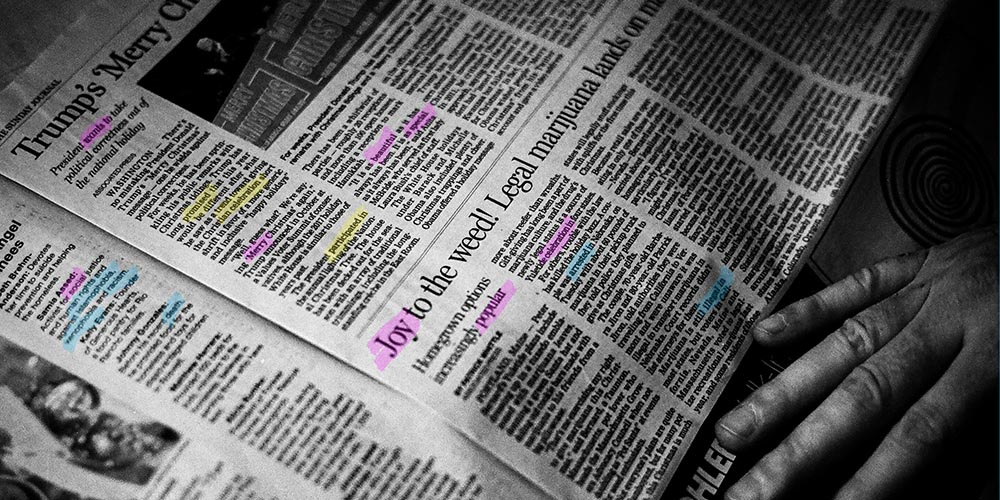
\includegraphics[width=1\linewidth,height=\textheight,keepaspectratio]{images/newspaper_content.jpg}
\caption{Content analysis of newspaper text.}
\end{figure}

This systematic process ensures the reliability, validity, and relevance of research findings, enabling scholars to make meaningful contributions to their fields.

\subsection*{Advancing Knowledge and Addressing Complex Issues}\label{advancing-knowledge-and-addressing-complex-issues}
\addcontentsline{toc}{subsection}{Advancing Knowledge and Addressing Complex Issues}

Social science research is indispensable for examining and addressing complex social issues. In mass communication and media studies, it provides insights into audience behavior, media effects, and cultural trends, shaping how we understand and interact with the world. By adhering to ethical principles and employing systematic methods, researchers ensure their work advances both theoretical knowledge and practical applications, benefiting industries and communities alike.

As you progress through this course, you will develop the skills necessary to engage in social science research. These skills will empower you to contribute meaningfully to the fields of mass communication and media studies, equipping you to analyze, interpret, and address the dynamic challenges of contemporary society.

\section{History of Social Science Research}\label{history-of-social-science-research}

The history of social science research reflects its growth as a systematic discipline focused on understanding human behavior, societal interactions, and cultural dynamics. Evolving from its philosophical roots, social science research has developed into an empirical and interdisciplinary field, combining qualitative and quantitative approaches to address complex social phenomena. Examining its historical trajectory reveals the milestones and challenges that have shaped its methodologies, ethics, and applications.

\subsection*{Early Foundations: From Philosophy to Empirical Inquiry}\label{early-foundations-from-philosophy-to-empirical-inquiry}
\addcontentsline{toc}{subsection}{Early Foundations: From Philosophy to Empirical Inquiry}

The origins of social science research lie in philosophy and early social observation. Thinkers such as Aristotle and Confucius pondered human behavior and societal structures, but their approaches were often speculative rather than systematic. The Enlightenment era introduced a shift toward reason and empirical inquiry, laying the groundwork for modern social science. Early pioneers like \textbf{Auguste Comte}, who coined the term ``sociology,'' and \textbf{Emile Durkheim} emphasized the use of scientific methods to study social phenomena. Their work established sociology as a distinct discipline, advocating for empirical research over abstract theorization.

\subsection*{The 19th and Early 20th Centuries: Methodological Advances}\label{the-19th-and-early-20th-centuries-methodological-advances}
\addcontentsline{toc}{subsection}{The 19th and Early 20th Centuries: Methodological Advances}

During the 19th and early 20th centuries, social science research matured through the adoption of structured methodologies and statistical analysis. The development of surveys enabled researchers to gather data on public opinion and behavior systematically. The \textbf{Chicago School of Sociology} was instrumental in advancing social science research, integrating fieldwork and qualitative methods like ethnography and participant observation to explore urban life and social structures.

This period also marked the diversification of research approaches, with the emergence of quantitative tools such as census analysis and correlation studies. These advancements allowed social scientists to study large-scale societal trends while addressing individual and community-level dynamics.

\subsection*{Mid-20th Century: Ethical Challenges and Theoretical Breakthroughs}\label{mid-20th-century-ethical-challenges-and-theoretical-breakthroughs}
\addcontentsline{toc}{subsection}{Mid-20th Century: Ethical Challenges and Theoretical Breakthroughs}

The mid-20th century was characterized by groundbreaking studies and significant ethical challenges. Notable examples include:

\begin{itemize}
\tightlist
\item
  \textbf{Stanley Milgram's Obedience Experiments}: These studies provided profound insights into human psychology by examining how individuals comply with authority, even when it conflicts with their moral values. However, they sparked debates about the psychological distress caused to participants.
\end{itemize}

\begin{figure}
\centering
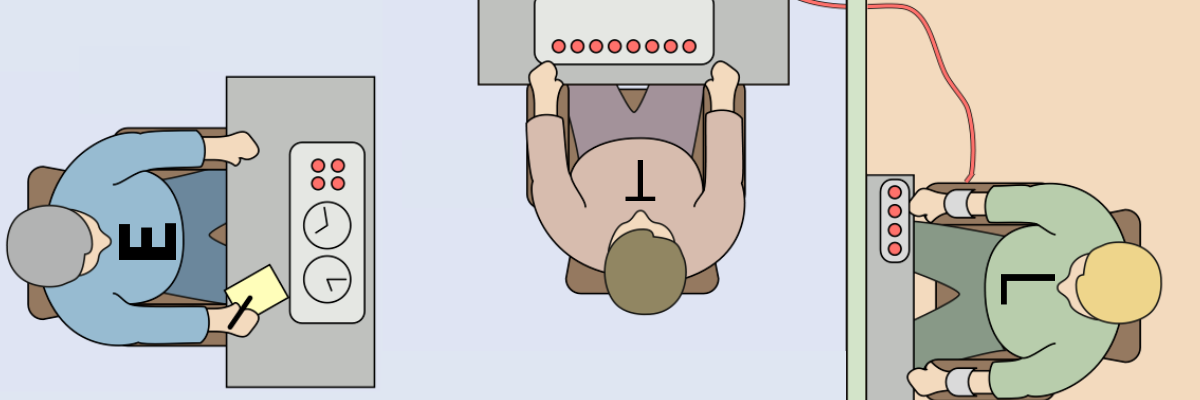
\includegraphics[width=1\linewidth,height=\textheight,keepaspectratio]{images/milgram_experiment.png}
\caption{Participants by role. T = Teacher, L = Learner, E = Experimenter.}
\end{figure}

\begin{itemize}
\tightlist
\item
  \textbf{Philip Zimbardo's Stanford Prison Experiment}: This research highlighted the influence of situational factors on behavior but faced criticism for the ethical issues surrounding participant harm and lack of informed consent.
\end{itemize}

\href{https://www.prisonexp.org/}{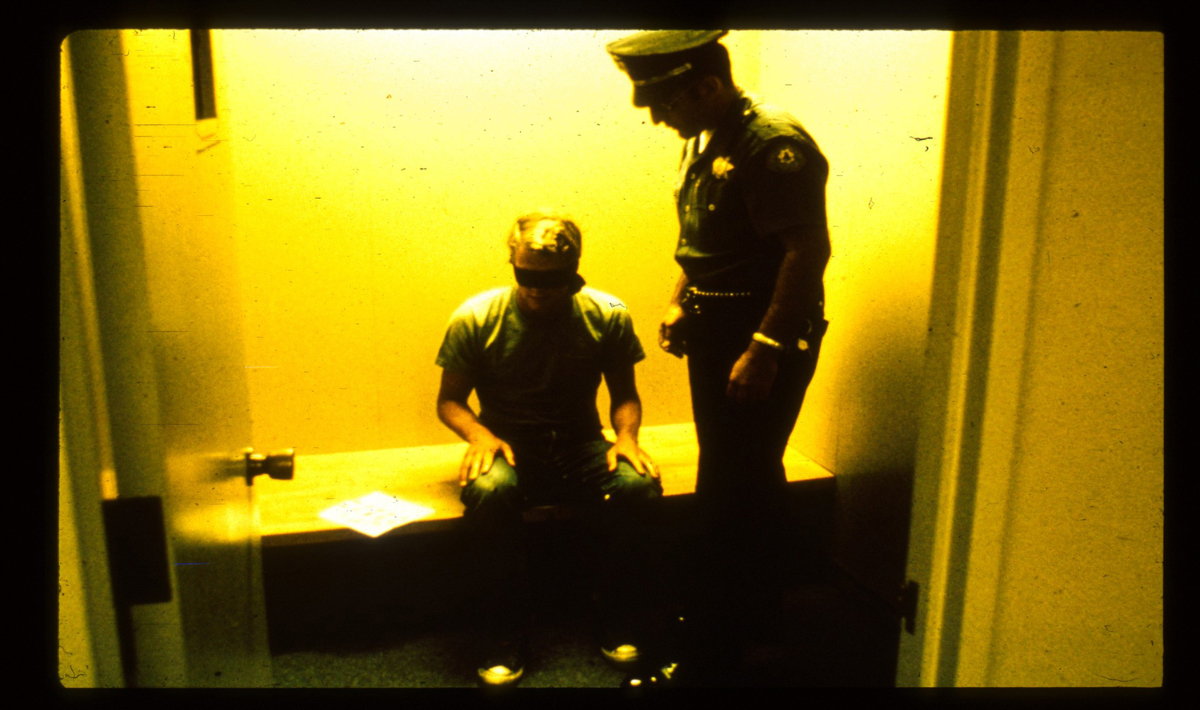
\includegraphics[width=1\linewidth,height=\textheight,keepaspectratio]{images/police-blindfolding.jpg}}

These ethical dilemmas prompted the establishment of formal guidelines, including the \textbf{Belmont Report}, which emphasized respect for persons, beneficence, and justice in research. Institutional Review Boards (IRBs) were created to ensure that studies involving human participants adhere to these principles.

\subsection*{Mass Communication Research in the Mid-20th Century}\label{mass-communication-research-in-the-mid-20th-century}
\addcontentsline{toc}{subsection}{Mass Communication Research in the Mid-20th Century}

The rise of mass media technologies, including radio, television, and newspapers, fueled significant advancements in communication research. Studies explored the effects of media on public opinion, behavior, and societal perceptions. Key contributions included:

\begin{itemize}
\tightlist
\item
  \textbf{Paul Lazarsfeld's Two-Step Flow Model}: This theory highlighted the role of opinion leaders in mediating media messages, demonstrating that mass communication often influences audiences indirectly.
\item
  \textbf{Walter Lippmann's Public Opinion}: Lippmann analyzed how media shapes societal perceptions, introducing concepts like the agenda-setting function of news.
\end{itemize}

These foundational studies laid the groundwork for contemporary media research, focusing on media framing, propaganda, and the relationship between media and cultural values.

\subsection*{The Digital Age: New Opportunities and Ethical Considerations}\label{the-digital-age-new-opportunities-and-ethical-considerations}
\addcontentsline{toc}{subsection}{The Digital Age: New Opportunities and Ethical Considerations}

The advent of the digital age has transformed social science research, introducing new tools and methodologies to study societal trends. Innovations such as:

\begin{itemize}
\tightlist
\item
  \textbf{Big Data Analysis}: Leveraging vast datasets to identify patterns in behavior, sentiment, and interactions.
\item
  \textbf{Social Media Research}: Employing digital ethnography, sentiment analysis, and network analysis to understand online communication and behavior.
\item
  \textbf{Algorithmic Analysis}: Examining the role of algorithms in shaping public discourse and media consumption.
\end{itemize}

\begin{figure}
\centering
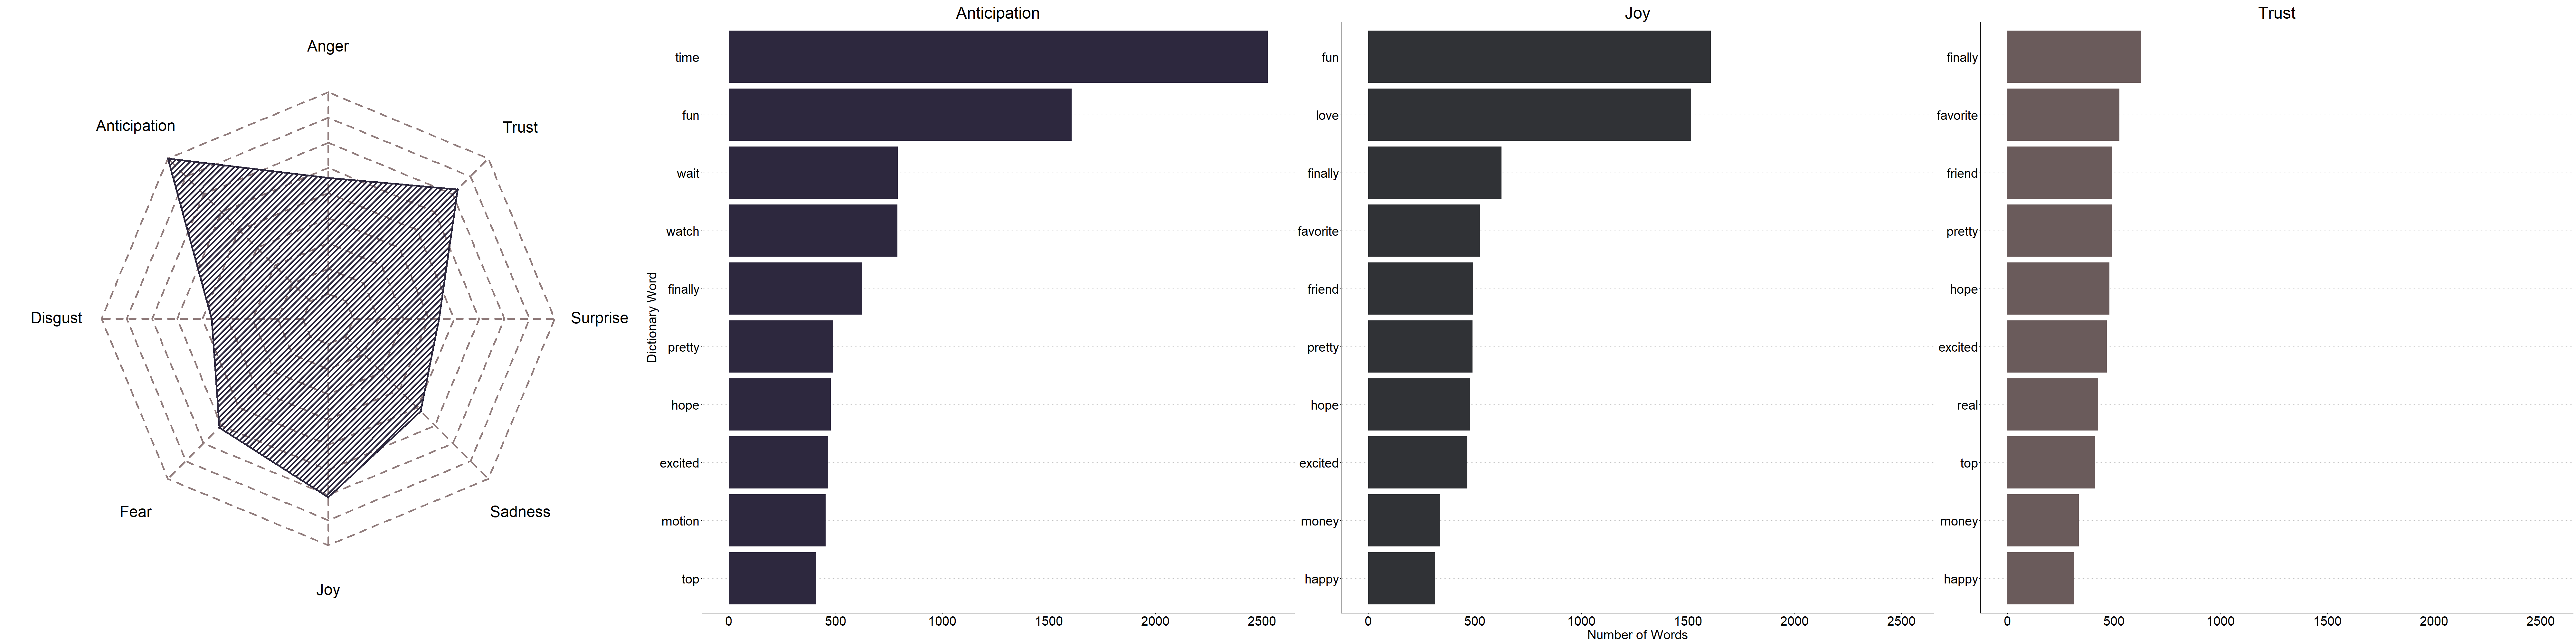
\includegraphics[width=1\linewidth,height=\textheight,keepaspectratio]{images/VR-Play-Emotion-MP.png}
\caption{Example of social media analysis using large datasets.}
\end{figure}

While these advancements have expanded the scope of research, they also raise ethical concerns, including data privacy, consent in online spaces, and algorithmic bias.

\subsection*{Contemporary Trends: Interdisciplinary and Applied Research}\label{contemporary-trends-interdisciplinary-and-applied-research}
\addcontentsline{toc}{subsection}{Contemporary Trends: Interdisciplinary and Applied Research}

Today, social science research is inherently interdisciplinary, integrating psychology, sociology, anthropology, political science, and economics to address pressing societal challenges. Key areas of focus include:

\begin{itemize}
\tightlist
\item
  \textbf{Misinformation and Media Literacy}: Developing strategies to counteract false information and promote critical engagement with media.
\item
  \textbf{Climate Change Communication}: Understanding how messaging influences public attitudes and policy support.
\item
  \textbf{Artificial Intelligence and Society}: Exploring how AI shapes public discourse, decision-making, and equity.
\end{itemize}

\section{Importance of Social Science Research}\label{importance-of-social-science-research}

Social science research is a cornerstone for understanding human behavior, societal dynamics, and the functioning of institutions. By employing systematic investigation, it provides invaluable insights into how individuals sand groups interact, how societal structures influence behavior, and how to address complex real-world challenges. This research is vital not only for advancing academic knowledge but also for informing policies, shaping communication strategies, and improving lives globally.

\subsection*{Evidence-Based Policymaking}\label{evidence-based-policymaking}
\addcontentsline{toc}{subsection}{Evidence-Based Policymaking}

One of the most critical contributions of social science research is its role in evidence-based policymaking. By identifying patterns in human behavior and societal trends, researchers provide data-driven recommendations to address pressing social issues such as poverty, inequality, and public health. For example:

\begin{itemize}
\tightlist
\item
  \textbf{Urban Development}: Research on housing policies has informed initiatives to improve living conditions in underserved communities.
\item
  \textbf{Education}: Studies on teaching strategies and curriculum design have enhanced learning outcomes, particularly for diverse and marginalized student populations.
\item
  \textbf{Public Health}: Investigations into healthcare access and preventive measures have shaped policies to mitigate health disparities and improve community well-being.
\end{itemize}

Through these applications, social science research directly impacts the quality of life and societal equity.

\subsection*{Insights into Communication and Media}\label{insights-into-communication-and-media}
\addcontentsline{toc}{subsection}{Insights into Communication and Media}

In the field of communication, social science research is indispensable for understanding how people consume, interpret, and respond to media. These insights empower media professionals to craft content that resonates with specific audiences and achieves desired outcomes. Key examples include:

\begin{itemize}
\tightlist
\item
  \textbf{Digital Marketing}: Survey data on social media usage helps advertisers design targeted campaigns that reach relevant demographics effectively.
\item
  \textbf{Message Framing}: Experiments reveal how the tone and structure of news stories influence public opinion and behavior.
\item
  \textbf{Content Strategy}: Media organizations leverage audience behavior studies to tailor programming, ensuring content meets viewer preferences and needs.
\end{itemize}

By grounding communication strategies in empirical research, professionals in advertising, journalism, and public relations can create impactful and ethical content.

\subsection*{Addressing Global Challenges}\label{addressing-global-challenges}
\addcontentsline{toc}{subsection}{Addressing Global Challenges}

Social science research is integral to tackling global issues, including climate change, public health crises, and social justice movements. Researchers explore topics such as:

\begin{itemize}
\tightlist
\item
  \textbf{Environmental Policies}: Studies on public attitudes toward sustainability guide efforts to promote green initiatives and behavior change.
\item
  \textbf{Pandemics}: Analyses of misinformation and its spread inform strategies to combat false narratives and build public trust.
\item
  \textbf{Social Movements}: Research on advocacy campaigns and protests identifies pathways to foster awareness, engagement, and collective action.
\end{itemize}

\href{https://drive.google.com/file/d/1JbErXZc2T6pSm-PsiFTY0j_1VE-MRds0/view}{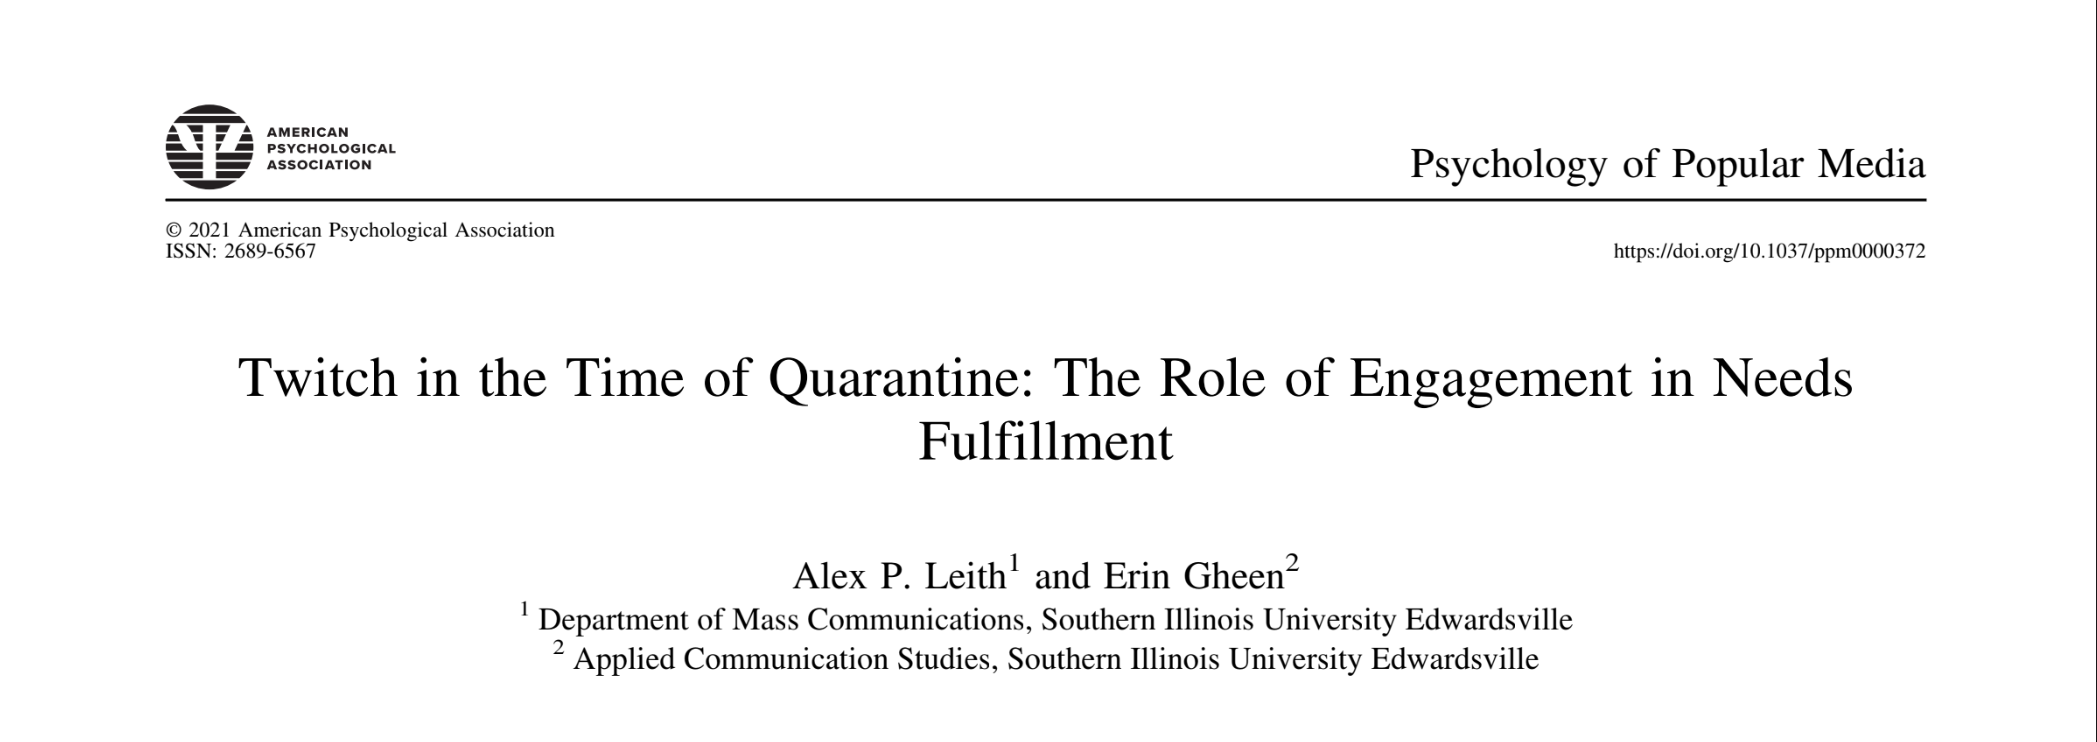
\includegraphics[width=1\linewidth,height=\textheight,keepaspectratio]{images/quarantine-twitch.png}}

By uncovering underlying dynamics and effective interventions, social science research equips stakeholders to address these challenges with evidence-based solutions.

\subsection*{Bridging Theory and Practice}\label{bridging-theory-and-practice}
\addcontentsline{toc}{subsection}{Bridging Theory and Practice}

A defining strength of social science research is its ability to bridge theory and practice. By testing and refining theories about human behavior and social systems, researchers generate knowledge that is both academically rigorous and practically applicable. Examples include:

\begin{itemize}
\tightlist
\item
  \textbf{Interpersonal Communication}: Research has informed conflict resolution strategies used in personal, organizational, and international contexts.
\item
  \textbf{Organizational Behavior}: Studies on motivation and leadership have led to improved workplace management practices, enhancing productivity and employee satisfaction.
\end{itemize}

This iterative relationship ensures that social science research remains relevant and impactful across disciplines and industries.

\subsection*{Ethical Foundations}\label{ethical-foundations}
\addcontentsline{toc}{subsection}{Ethical Foundations}

The credibility of social science research is rooted in its adherence to ethical principles, including:

\begin{itemize}
\tightlist
\item
  \textbf{Informed Consent}: Ensuring participants understand the purpose, risks, and benefits of the research.
\item
  \textbf{Confidentiality}: Protecting the privacy of participants and their data.
\item
  \textbf{Equity}: Avoiding exploitation and ensuring fair representation of all groups in research studies.
\end{itemize}

These ethical commitments are particularly important when studying sensitive topics or vulnerable populations, enhancing public trust in research findings.

\subsection*{Empowering Mass Communication and Media Studies}\label{empowering-mass-communication-and-media-studies}
\addcontentsline{toc}{subsection}{Empowering Mass Communication and Media Studies}

In mass communication and media studies, social science research is essential for navigating the rapidly changing media landscape. It enables professionals to:

\begin{itemize}
\tightlist
\item
  \textbf{Anticipate Trends}: Predict shifts in audience preferences and media consumption patterns.
\item
  \textbf{Engage Effectively}: Design content and campaigns that resonate with target audiences.
\item
  \textbf{Innovate}: Develop new methods for understanding and addressing societal challenges through media.
\end{itemize}

\section{Types of Social Science Research}\label{types-of-social-science-research}

Social science research employs diverse methodologies to investigate human behavior, societal structures, and cultural phenomena. These methodologies are categorized into three primary types: \textbf{qualitative}, \textbf{quantitative}, and \textbf{mixed methods} research. Each type addresses distinct research questions and offers unique insights, making them indispensable tools for understanding the complexities of individuals and society.

\subsection*{Qualitative Research: Exploring Depth and Meaning}\label{qualitative-research-exploring-depth-and-meaning}
\addcontentsline{toc}{subsection}{Qualitative Research: Exploring Depth and Meaning}

\textbf{Qualitative research} focuses on exploring the rich, detailed contexts and meanings behind social phenomena. Rather than relying on numerical data, this approach seeks to answer ``why'' and ``how'' questions, offering deep insights into personal experiences, cultural norms, and group dynamics.

\subsubsection*{Common Methods:}\label{common-methods}
\addcontentsline{toc}{subsubsection}{Common Methods:}

\begin{itemize}
\tightlist
\item
  \textbf{In-Depth Interviews}: Conversations designed to explore participants' perspectives in detail.
\item
  \textbf{Focus Groups}: Facilitated discussions that reveal group dynamics and collective viewpoints.
\item
  \textbf{Ethnography}: Immersive observation and interaction within a cultural or social group.
\end{itemize}

\begin{figure}
\centering
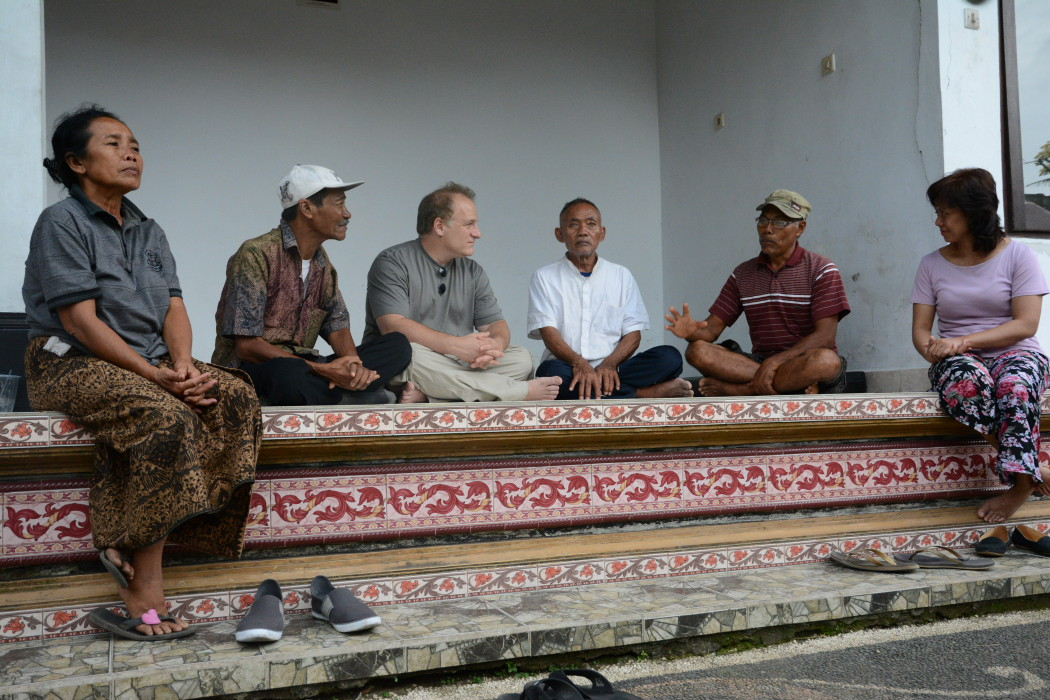
\includegraphics[width=1\linewidth,height=\textheight,keepaspectratio]{images/part-observation.jpg}
\caption{Example of researcher conducting ethnography.}
\end{figure}

\subsubsection*{Example Applications:}\label{example-applications}
\addcontentsline{toc}{subsubsection}{Example Applications:}

\begin{itemize}
\tightlist
\item
  Studying how individuals construct identities on social media.
\item
  Exploring how cultural values influence audience interpretations of media content.
\end{itemize}

\subsubsection*{Strengths:}\label{strengths}
\addcontentsline{toc}{subsubsection}{Strengths:}

\begin{itemize}
\tightlist
\item
  Provides nuanced, context-rich perspectives.
\item
  Captures the complexity of human experiences.
\end{itemize}

\subsubsection*{Limitations:}\label{limitations}
\addcontentsline{toc}{subsubsection}{Limitations:}

\begin{itemize}
\tightlist
\item
  Findings are typically context-specific and may not be easily generalizable.
\item
  Often relies on smaller, purposive samples rather than large datasets.
\end{itemize}

Qualitative research is particularly valuable in mass communication for analyzing textual, visual, and interactive media elements that shape cultural narratives and audience perceptions.

\subsection*{Quantitative Research: Measuring and Generalizing}\label{quantitative-research-measuring-and-generalizing}
\addcontentsline{toc}{subsection}{Quantitative Research: Measuring and Generalizing}

\textbf{Quantitative research} emphasizes numerical measurement and statistical analysis to test hypotheses, identify patterns, and generalize findings to broader populations. This approach answers ``what,'' ``where,'' and ``when'' questions, offering the reliability of structured data collection.

\subsubsection*{Common Methods:}\label{common-methods-1}
\addcontentsline{toc}{subsubsection}{Common Methods:}

\begin{itemize}
\tightlist
\item
  \textbf{Surveys}: Questionnaires designed to gather data from a large number of respondents.
\item
  \textbf{Experiments}: Controlled studies to test causal relationships.
\item
  \textbf{Content Analysis}: Systematic coding and quantification of media content.
\end{itemize}

\begin{figure}
\centering
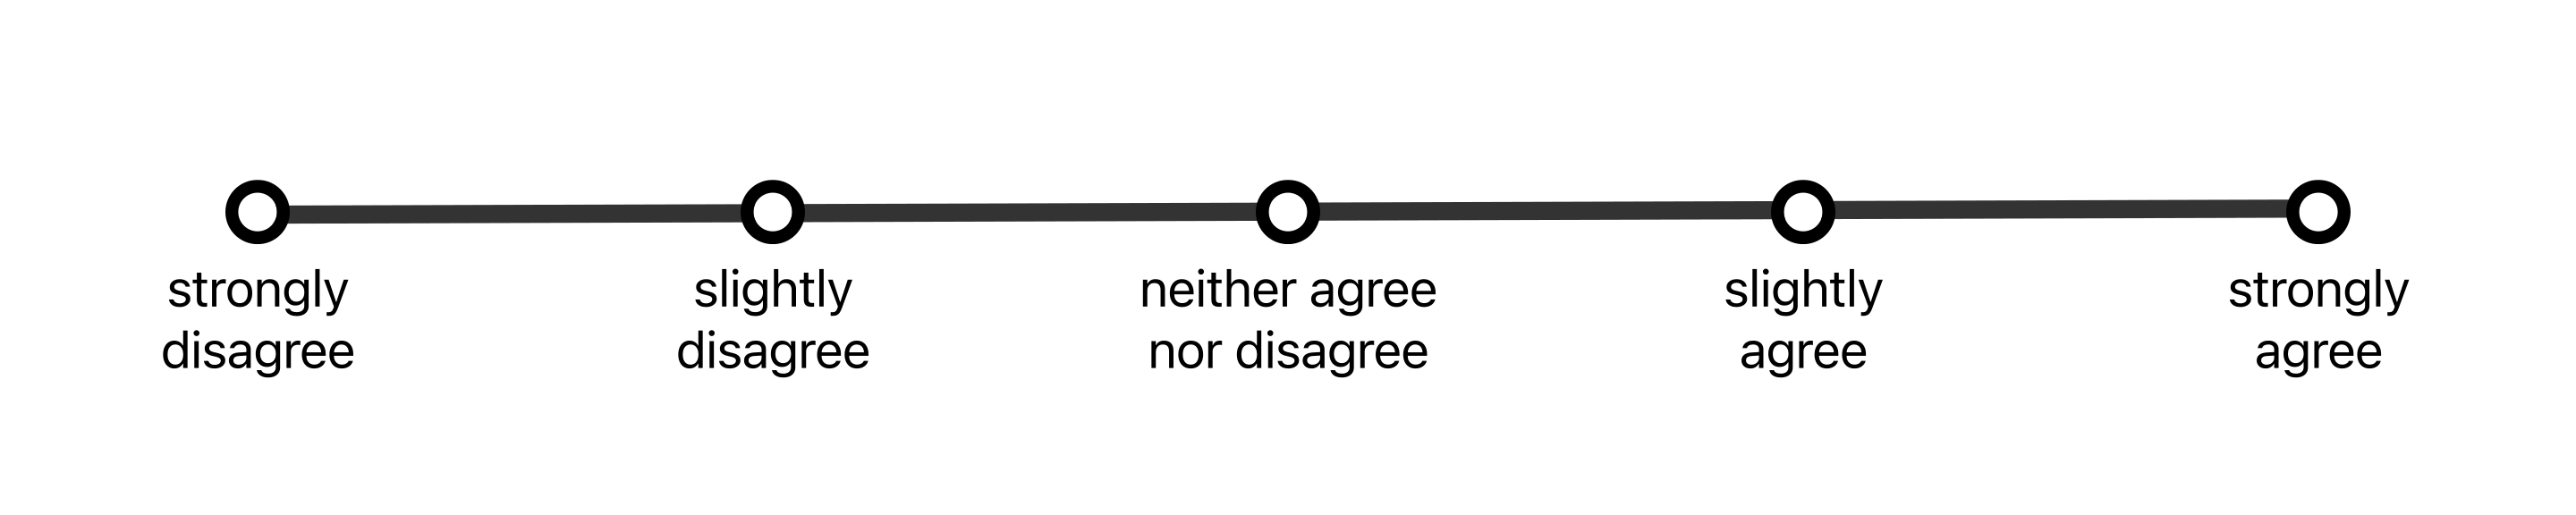
\includegraphics[width=1\linewidth,height=\textheight,keepaspectratio]{images/likert-scale.png}
\caption{Common Likert-type scale responses.}
\end{figure}

\subsubsection*{Example Applications:}\label{example-applications-1}
\addcontentsline{toc}{subsubsection}{Example Applications:}

\begin{itemize}
\tightlist
\item
  Measuring the relationship between social media usage and mental health outcomes.
\item
  Analyzing the prevalence of gender stereotypes in television advertising.
\end{itemize}

\subsubsection*{Strengths:}\label{strengths-1}
\addcontentsline{toc}{subsubsection}{Strengths:}

\begin{itemize}
\tightlist
\item
  Enables statistically valid inferences across diverse populations.
\item
  Provides breadth and replicability through standardized measures.
\end{itemize}

\subsubsection*{Limitations:}\label{limitations-1}
\addcontentsline{toc}{subsubsection}{Limitations:}

\begin{itemize}
\tightlist
\item
  May overlook the contextual and nuanced aspects of phenomena.
\item
  Lacks the depth of insight offered by qualitative methods.
\end{itemize}

Quantitative research is widely used in mass communication to assess audience behavior, measure media effects, and identify trends in media consumption and representation.

\subsection*{Mixed Methods Research: Bridging Breadth and Depth}\label{mixed-methods-research-bridging-breadth-and-depth}
\addcontentsline{toc}{subsection}{Mixed Methods Research: Bridging Breadth and Depth}

\textbf{Mixed methods research} combines qualitative and quantitative approaches to offer a comprehensive understanding of complex research questions. This integrative approach leverages the strengths of both methodologies, addressing multifaceted issues with greater depth and breadth.

\subsubsection*{Common Designs:}\label{common-designs}
\addcontentsline{toc}{subsubsection}{Common Designs:}

\begin{itemize}
\tightlist
\item
  \textbf{Sequential Explanatory}: Quantitative data is collected first to identify trends, followed by qualitative exploration to uncover underlying reasons.
\item
  \textbf{Concurrent Triangulation}: Quantitative and qualitative data are collected simultaneously to validate and enrich findings.
\item
  \textbf{Embedded Design}: One method is embedded within the other to address complementary aspects of a research question.
\end{itemize}

\subsubsection*{Example Applications:}\label{example-applications-2}
\addcontentsline{toc}{subsubsection}{Example Applications:}

\begin{itemize}
\tightlist
\item
  Assessing the effectiveness of public health campaigns by analyzing survey data on audience reach (quantitative) and conducting interviews to explore message interpretation (qualitative).
\item
  Investigating media framing by quantifying patterns in news coverage and exploring journalists' perspectives through interviews.
\end{itemize}

\subsubsection*{Strengths:}\label{strengths-2}
\addcontentsline{toc}{subsubsection}{Strengths:}

\begin{itemize}
\tightlist
\item
  Provides a holistic perspective by integrating numerical trends with contextual understanding.
\item
  Allows researchers to address complex questions from multiple angles.
\end{itemize}

\subsubsection*{Limitations:}\label{limitations-2}
\addcontentsline{toc}{subsubsection}{Limitations:}

\begin{itemize}
\tightlist
\item
  Requires significant resources, expertise, and time to manage diverse data types.
\item
  Demands careful integration of findings to ensure coherence and validity.
\end{itemize}

Mixed methods research is particularly valuable in mass communication for studying issues like media effects, audience engagement, and the intersection of technology and culture.

\subsection*{Choosing the Right Approach}\label{choosing-the-right-approach}
\addcontentsline{toc}{subsection}{Choosing the Right Approach}

Each type of social science research has distinct advantages and limitations, making the choice of approach crucial for a study's success.

\begin{itemize}
\tightlist
\item
  \textbf{Qualitative methods} excel in capturing depth and context but lack generalizability.
\item
  \textbf{Quantitative approaches} offer statistical rigor and replicability but may overlook nuances.
\item
  \textbf{Mixed methods research} bridges these gaps, providing a balanced perspective but requiring additional resources and expertise.
\end{itemize}

In \textbf{mass communication and media studies}, these methodologies are applied to examine a wide range of phenomena, from the cultural significance of media representations to the effectiveness of communication strategies. As researchers, understanding the strengths and limitations of each approach will empower you to select the most appropriate methods, ensuring robust, meaningful contributions to academic knowledge and practical solutions.

\section{The Research Process}\label{the-research-process}

The research process in social science is a systematic framework designed to ensure rigor, validity, and reliability in studying human behavior and societal dynamics. By following a structured sequence of interconnected steps, researchers can address complex questions, test hypotheses, and contribute to the growing body of knowledge in their field. While the specifics may vary across disciplines and methodologies, the core stages of the research process remain consistent and provide a robust foundation for effective inquiry.

\subsection*{Step 1: Identifying the Research Question}\label{step-1-identifying-the-research-question}
\addcontentsline{toc}{subsection}{Step 1: Identifying the Research Question}

The research process begins with identifying a research question or problem. This step involves pinpointing a gap in existing knowledge, addressing a pressing issue, or exploring a new area of interest. A well-defined research question serves as the cornerstone of the study, shaping its direction and scope. For example, a mass communication researcher might ask, \emph{``How does social media influence political engagement among young adults?''}

To refine the research question:

\begin{itemize}
\tightlist
\item
  \textbf{Preliminary Exploration}: Review existing studies to ensure the question is feasible and significant.
\item
  \textbf{Clarity and Focus}: Ensure the question is specific enough to guide the research but broad enough to allow meaningful investigation.
\end{itemize}

\subsection*{Step 2: Reviewing the Literature}\label{step-2-reviewing-the-literature}
\addcontentsline{toc}{subsection}{Step 2: Reviewing the Literature}

A comprehensive literature review is the next step, enabling researchers to understand what is already known about their topic. This involves:

\begin{itemize}
\tightlist
\item
  \textbf{Synthesizing Prior Research}: Analyzing previous findings, theories, and methodologies to identify trends and gaps.
\item
  \textbf{Establishing Context}: Positioning the research question within a broader academic framework.
\item
  \textbf{Avoiding Redundancy}: Building on existing knowledge while ensuring the study offers unique contributions.
\end{itemize}

For example, in media studies, this might include examining existing work on media framing, audience behavior, or misinformation.

\begin{figure}
\centering
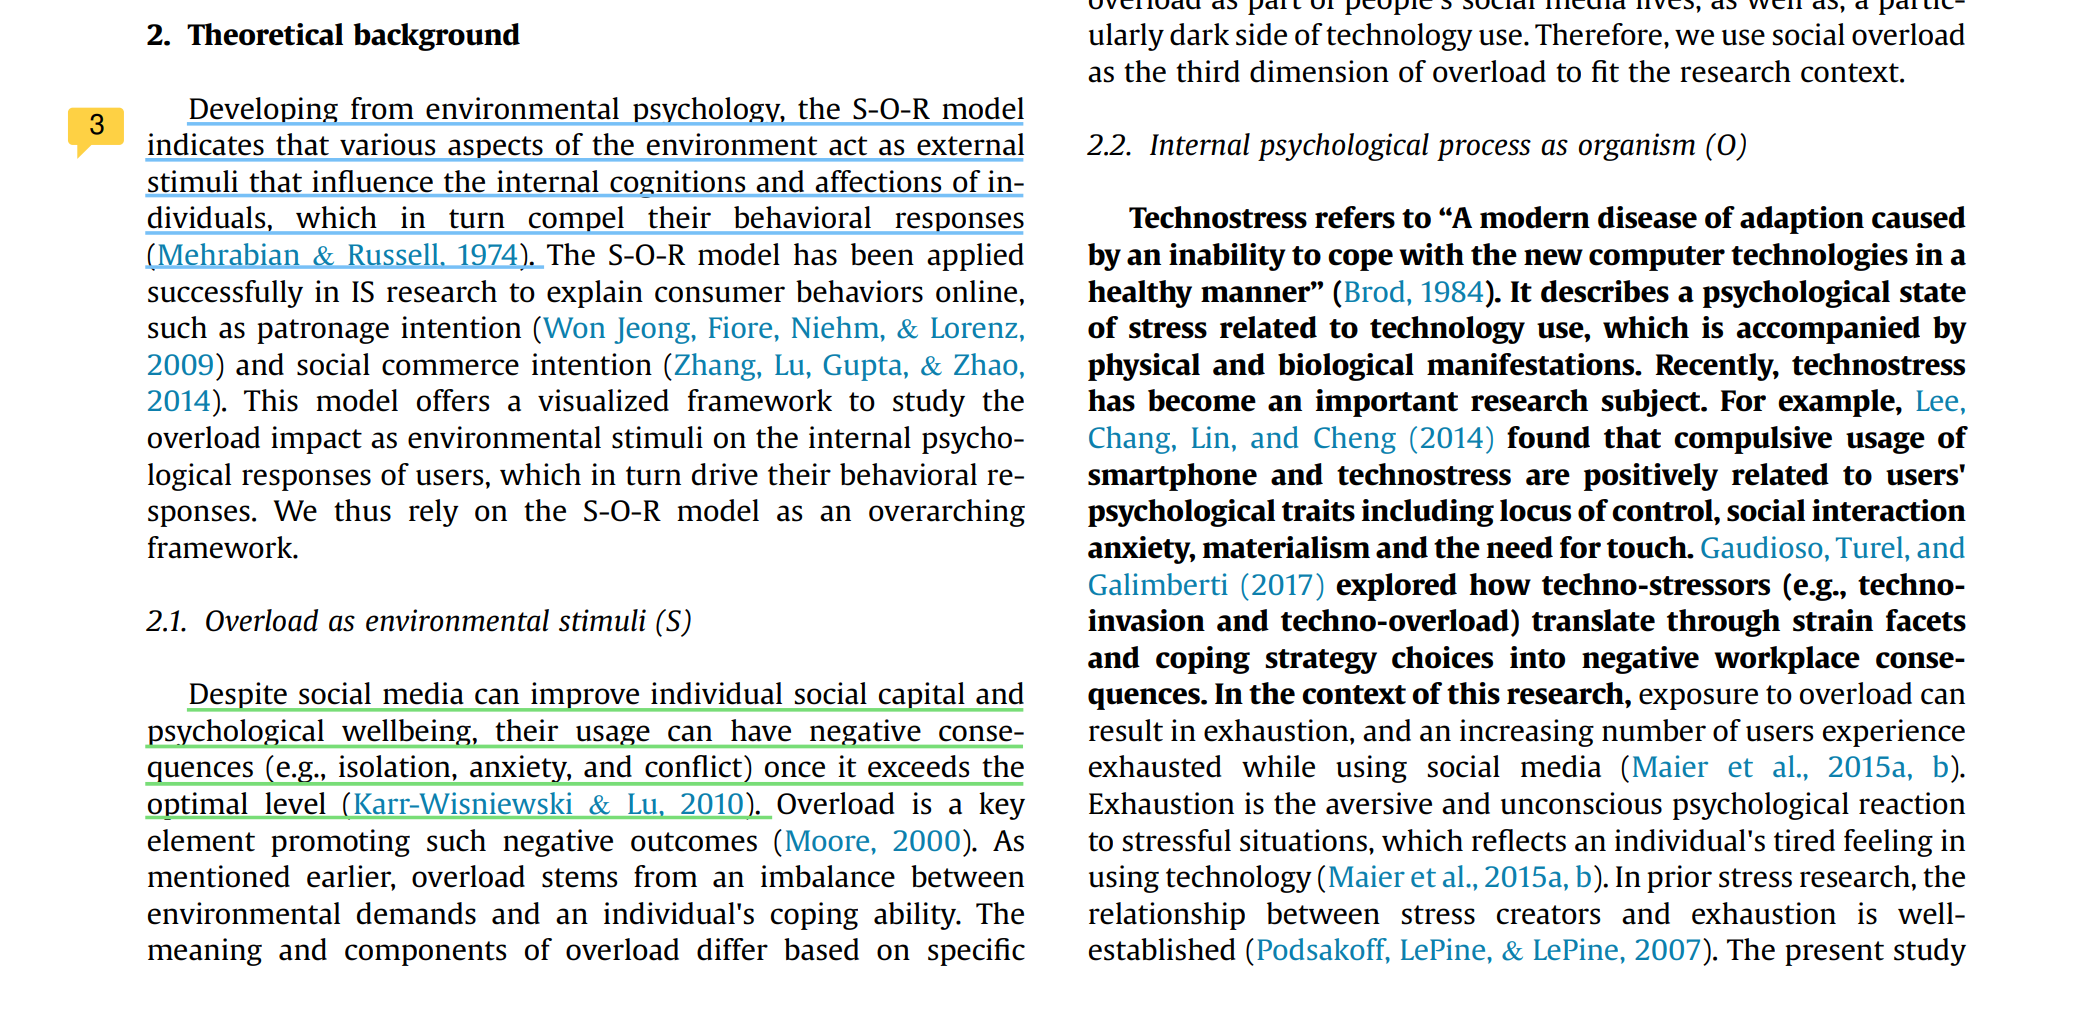
\includegraphics[width=1\linewidth,height=\textheight,keepaspectratio]{images/annotated_manuscript.png}
\caption{Example of manuscript annotation.}
\end{figure}

\subsection*{Step 3: Designing the Study}\label{step-3-designing-the-study}
\addcontentsline{toc}{subsection}{Step 3: Designing the Study}

Study design is critical to ensuring the research effectively addresses the research question. This stage involves:

\begin{itemize}
\tightlist
\item
  \textbf{Choosing a Methodology}: Selecting qualitative, quantitative, or mixed methods based on the type of data needed.
\item
  \textbf{Defining Variables}: Clearly identifying independent, dependent, and control variables.
\item
  \textbf{Sampling}: Choosing an appropriate population or sample size to ensure validity and generalizability.
\item
  \textbf{Developing Procedures}: Outlining steps for data collection, including timelines and resources.
\end{itemize}

Example: A researcher studying audience reactions to political advertisements might use:

\begin{itemize}
\tightlist
\item
  \textbf{Experiments}: To observe reactions under controlled conditions.
\item
  \textbf{Surveys}: To gather broader demographic insights.
\end{itemize}

\subsection*{Step 4: Data Collection}\label{step-4-data-collection}
\addcontentsline{toc}{subsection}{Step 4: Data Collection}

Data collection is where researchers gather the information needed to address their research question. This phase varies depending on the chosen methodology:

\begin{itemize}
\tightlist
\item
  \textbf{Qualitative Methods}: Interviews, focus groups, or ethnography to capture detailed narratives and experiences.
\item
  \textbf{Quantitative Methods}: Surveys, experiments, or content analysis to gather structured numerical data.
\item
  \textbf{Mixed Methods}: Combining qualitative and quantitative approaches for a comprehensive understanding.
\end{itemize}

Ethical considerations are paramount during data collection. For instance:

\begin{itemize}
\tightlist
\item
  Obtain \textbf{informed consent}.
\item
  Ensure \textbf{confidentiality} and \textbf{privacy}, particularly for sensitive topics like political attitudes or media consumption.
\end{itemize}

\subsection*{Step 5: Data Analysis}\label{step-5-data-analysis}
\addcontentsline{toc}{subsection}{Step 5: Data Analysis}

Once data is collected, researchers analyze it to identify patterns, test hypotheses, and draw meaningful conclusions:

\begin{itemize}
\tightlist
\item
  \textbf{Quantitative Analysis}: Statistical methods are used to calculate measures such as central tendency, variance, correlations, or regression models.
\item
  \textbf{Qualitative Analysis}: Data is coded and thematically analyzed to uncover insights into participants' experiences and perspectives.
\item
  \textbf{Mixed Methods Integration}: Numerical trends are combined with contextual depth to create a holistic understanding.
\end{itemize}

\begin{figure}
\centering
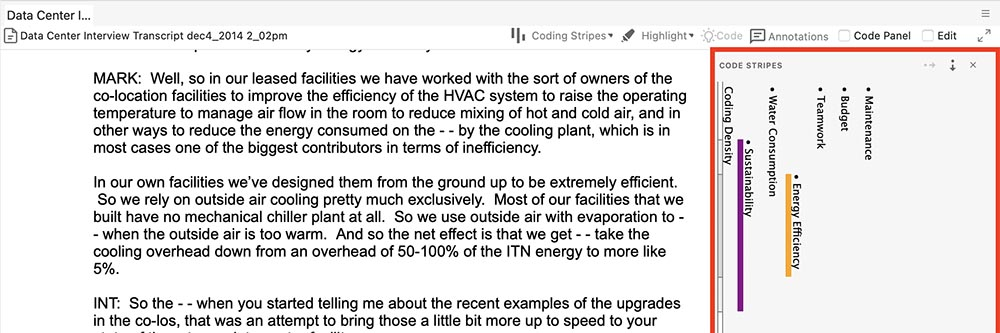
\includegraphics[width=1\linewidth,height=\textheight,keepaspectratio]{images/qual_content.jpg}
\caption{Some qualitative content analysis.}
\end{figure}

Example: A study on media consumption might:

\begin{itemize}
\tightlist
\item
  Use surveys to identify trends in viewing habits (quantitative).
\item
  Conduct interviews to explore why participants favor specific media platforms (qualitative).
\end{itemize}

\subsection*{Step 6: Reporting Findings}\label{step-6-reporting-findings}
\addcontentsline{toc}{subsection}{Step 6: Reporting Findings}

The final step is to communicate findings clearly and effectively. Researchers present their results through:

\begin{itemize}
\tightlist
\item
  \textbf{Academic Publications}: Peer-reviewed journals and conference presentations.
\item
  \textbf{Industry Reports}: Practical recommendations for stakeholders.
\item
  \textbf{Public Communication}: Summaries or infographics tailored to broader audiences.
\end{itemize}

Key components of reporting include:

\begin{itemize}
\tightlist
\item
  \textbf{Results and Implications}: Highlighting the study's significance and relevance.
\item
  \textbf{Limitations}: Acknowledging potential constraints or biases in the research.
\item
  \textbf{Future Directions}: Suggesting areas for further exploration.
\end{itemize}

In mass communication, findings might guide strategies for improving audience engagement, combating misinformation, or refining media campaigns.

\subsection*{The Role of Ethics}\label{the-role-of-ethics}
\addcontentsline{toc}{subsection}{The Role of Ethics}

Ethics underpins every stage of the research process. Researchers must:

\begin{itemize}
\tightlist
\item
  Respect participants' \textbf{rights and autonomy}.
\item
  Minimize harm while maximizing societal benefits.
\item
  Adhere to principles of \textbf{informed consent}, \textbf{confidentiality}, and \textbf{equity}.
\end{itemize}

By following these ethical guidelines, researchers enhance the credibility of their work and foster trust with the communities they study.

\subsection*{Dynamic and Iterative Nature of the Process}\label{dynamic-and-iterative-nature-of-the-process}
\addcontentsline{toc}{subsection}{Dynamic and Iterative Nature of the Process}

The research process is rarely linear; it often requires adjustments and refinements at each stage. Researchers might revisit their research question after reviewing literature or refine data collection methods based on early findings. This dynamic approach ensures flexibility and adaptability in addressing complex social phenomena.

\section{Research Ethics}\label{research-ethics}

Research ethics serve as the foundation of responsible social science inquiry, ensuring that studies are conducted with respect, fairness, and integrity. Ethical principles guide every stage of the research process---from formulating research questions to disseminating findings---while prioritizing the rights and well-being of participants. By adhering to ethical standards, researchers maintain the integrity of their work, uphold public trust, and contribute positively to societal understanding. These considerations are especially critical in social science research, where studies often engage with vulnerable populations, sensitive topics, and issues of significant societal impact.

\subsection*{The Historical Evolution of Research Ethics}\label{the-historical-evolution-of-research-ethics}
\addcontentsline{toc}{subsection}{The Historical Evolution of Research Ethics}

The importance of research ethics has been shaped by historical examples of unethical practices that exposed the devastating consequences of disregarding ethical principles. Notable cases include:

\begin{itemize}
\tightlist
\item
  \textbf{The Tuskegee Syphilis Study}: Conducted from 1932 to 1972, this study withheld treatment from African American men with syphilis to observe the disease's progression, causing unnecessary suffering and violating participants' rights.
\item
  \textbf{The Stanford Prison Experiment}: This 1971 study simulated a prison environment, resulting in psychological harm to participants due to a lack of safeguards and oversight.
\end{itemize}

\begin{figure}
\centering
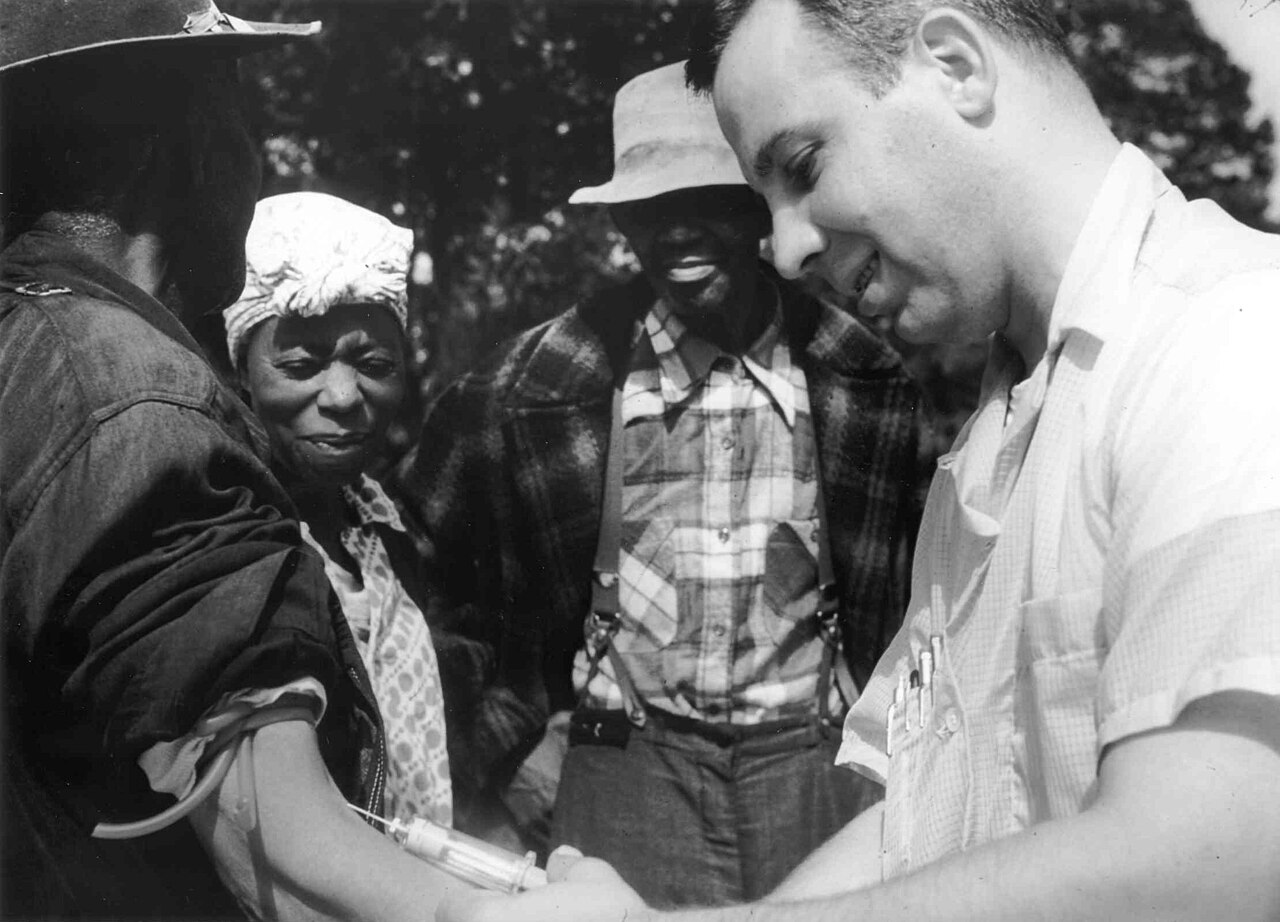
\includegraphics[width=1\linewidth,height=\textheight,keepaspectratio]{images/Tuskegee-syphilis-study.jpg}
\caption{Tuskegee Syphilis Study}
\end{figure}

These and similar instances led to the development of foundational ethical frameworks, such as:

\begin{itemize}
\tightlist
\item
  \textbf{The Belmont Report}: Established three core principles:

  \begin{enumerate}
  \def\labelenumi{\arabic{enumi}.}
  \tightlist
  \item
    \textbf{Respect for Persons}: Protect participants' autonomy by obtaining informed consent and ensuring they understand the research.
  \item
    \textbf{Beneficence}: Minimize risks and maximize benefits for participants and society.
  \item
    \textbf{Justice}: Ensure fair participant selection and equitable distribution of research risks and rewards.
  \end{enumerate}
\end{itemize}

These principles remain central to contemporary ethical standards and the oversight provided by \textbf{Institutional Review Boards (IRBs)}.

\subsection*{The Role of Ethical Principles in Research}\label{the-role-of-ethical-principles-in-research}
\addcontentsline{toc}{subsection}{The Role of Ethical Principles in Research}

Ethical principles are embedded in every stage of the research process, guiding decisions and practices to ensure that studies are conducted responsibly and respectfully.

\subsubsection*{Planning and Review}\label{planning-and-review}
\addcontentsline{toc}{subsubsection}{Planning and Review}

Ethical research begins with careful planning and thorough review:

\begin{itemize}
\tightlist
\item
  \textbf{Institutional Review Boards (IRBs)}: IRBs evaluate research proposals to ensure compliance with ethical standards. Researchers must demonstrate:

  \begin{itemize}
  \tightlist
  \item
    The study addresses meaningful questions.
  \item
    The methodology is sound and minimizes risks.
  \item
    Safeguards are in place to protect privacy and confidentiality.
  \end{itemize}
\end{itemize}

Example: In a study on media consumption, anonymizing survey responses ensures that participants' identities are protected, especially when handling sensitive demographic or behavioral data.

\subsubsection*{Data Collection}\label{data-collection}
\addcontentsline{toc}{subsubsection}{Data Collection}

The data collection phase demands careful consideration to uphold participants' rights:

\begin{itemize}
\tightlist
\item
  \textbf{Informed Consent}: Participants must be fully aware of the research purpose, procedures, risks, and benefits, and voluntarily agree to participate.
\item
  \textbf{Confidentiality}: Personal information must be securely stored and shared only when necessary.
\item
  \textbf{Minimizing Harm}: Researchers must avoid causing physical, emotional, or social harm, particularly when exploring sensitive topics like political opinions or media consumption habits.
\end{itemize}

\subsubsection*{Analysis and Reporting}\label{analysis-and-reporting}
\addcontentsline{toc}{subsubsection}{Analysis and Reporting}

Ethics extend beyond data collection to the analysis and dissemination of findings:

\begin{itemize}
\tightlist
\item
  \textbf{Honesty and Transparency}: Researchers must report findings truthfully, avoiding practices such as data manipulation, selective reporting, or plagiarism.
\item
  \textbf{Reproducibility}: Providing detailed methodologies allows other researchers to replicate studies, verify findings, and build on previous work.
\item
  \textbf{Avoiding Harmful Misrepresentation}: In media studies, where research can shape public discourse and policy, ethical reporting is critical to prevent misinformation or misinterpretation of data.
\end{itemize}

\subsection*{Ethical Challenges in the Digital Age}\label{ethical-challenges-in-the-digital-age}
\addcontentsline{toc}{subsection}{Ethical Challenges in the Digital Age}

The rise of digital research introduces unique ethical considerations:

\begin{itemize}
\tightlist
\item
  \textbf{Online Research and Privacy}: Social media platforms offer rich data sources but raise concerns about consent and privacy. Researchers analyzing publicly available posts must consider whether users perceive their data as private and ensure that findings do not harm individuals or communities.
\item
  \textbf{Big Data and Algorithmic Bias}: Ethical challenges arise in the use of large datasets and machine learning algorithms, particularly when biases in data collection or analysis perpetuate inequalities.
\item
  \textbf{Informed Consent in Digital Spaces}: Obtaining clear consent becomes more complex in online settings where users may not fully understand how their data will be used.
\end{itemize}

\subsection*{Cultural and Contextual Considerations}\label{cultural-and-contextual-considerations}
\addcontentsline{toc}{subsection}{Cultural and Contextual Considerations}

Ethics intersect with cultural and contextual factors, particularly in global or interdisciplinary research:

\begin{itemize}
\tightlist
\item
  \textbf{Respect for Cultural Norms}: Researchers must honor the values and practices of the populations they study.
\item
  \textbf{Engaging Stakeholders}: Collaborating with community leaders and participants ensures that research aligns with local priorities and fosters trust.
\item
  \textbf{Inclusive Reporting}: Sharing findings in accessible formats ensures that diverse audiences benefit from the research.
\end{itemize}

\subsection*{The Importance of Research Ethics for Students}\label{the-importance-of-research-ethics-for-students}
\addcontentsline{toc}{subsection}{The Importance of Research Ethics for Students}

For students in media and communication studies, understanding research ethics is a critical skill that enhances the credibility, quality, and impact of their work. Ethical research practices:

\begin{itemize}
\tightlist
\item
  Build \textbf{trust} between researchers and participants.
\item
  Ensure studies contribute \textbf{positively} to societal understanding.
\item
  Establish a foundation for conducting research that is both \textbf{rigorous} and \textbf{respectful}.
\end{itemize}

As emerging researchers, you will navigate complex ethical landscapes involving digital privacy, cultural diversity, and the power of media to shape public perception. By adhering to ethical principles, you can conduct studies that advance knowledge responsibly while fostering trust and integrity within your field.

\chapter{The Many SIUE Resources}\label{the-many-siue-resources}

\section{Introduction to SIUE Resources}\label{introduction-to-siue-resources}

Southern Illinois University Edwardsville (SIUE) offers a comprehensive suite of academic and research resources designed to empower students and faculty in their pursuit of knowledge, innovation, and professional development. These resources are invaluable for navigating the complexities of university-level research, especially for new learners transitioning to advanced academic environments. From specialized research tools to collaborative programs, SIUE fosters an environment that supports creativity, critical thinking, and scholarly achievement.

\subsection*{Why Engage with SIUE Resources?}\label{why-engage-with-siue-resources}
\addcontentsline{toc}{subsection}{Why Engage with SIUE Resources?}

Engaging with the resources at SIUE is not just about meeting academic requirements---it is about building a foundation for lifelong learning and professional success. Whether refining writing skills, managing complex data analyses, or conducting ethically sound research, these resources ensure students and faculty have the tools and support necessary to excel. By leveraging these opportunities, researchers gain not only technical proficiency but also the confidence to address complex challenges and contribute to their fields meaningfully.

\subsection*{Highlights of SIUE's Academic Support Ecosystem}\label{highlights-of-siues-academic-support-ecosystem}
\addcontentsline{toc}{subsection}{Highlights of SIUE's Academic Support Ecosystem}

\begin{enumerate}
\def\labelenumi{\arabic{enumi}.}
\tightlist
\item
  \textbf{Lovejoy Library}: A state-of-the-art library system offering access to a vast collection of physical and digital resources, personalized research support, and advanced technological tools for data analysis and visualization.
\item
  \textbf{SIUE Writing Center}: A dedicated space for developing academic writing skills through one-on-one tutoring, workshops, and resources tailored to student needs, including help with citations and academic formatting.
\item
  \textbf{Institutional Review Board (IRB)}: Ensuring ethical and responsible research practices, the IRB provides oversight, guidance, and training for studies involving human participants.
\item
  \textbf{Office of Research and Projects (ORP)}: A cornerstone for research funding, compliance, and project management, the ORP supports researchers at every stage, from proposal development to post-award administration.
\item
  \textbf{Zotero and Citation Tools}: Streamlining citation management and academic integrity, these tools simplify the organization of sources and integration into research projects.
\item
  \textbf{Information Technology Services (ITS)}: Offering cutting-edge computing resources, including high-performance computing systems, specialized software, and cyberinfrastructure, ITS supports advanced research and analysis.
\item
  \textbf{Undergraduate Research and Creative Activities (URCA)}: Providing hands-on research opportunities, URCA connects students with faculty mentors, fostering skill development and professional growth.
\item
  \textbf{IRIS Center}: A hub for interdisciplinary research and innovation, the IRIS Center facilitates collaboration across technology, humanities, and social sciences.
\end{enumerate}

\subsection*{Preparing for Success}\label{preparing-for-success}
\addcontentsline{toc}{subsection}{Preparing for Success}

The resources provided by SIUE reflect its commitment to supporting student and faculty success. By engaging early and often with these tools and services, individuals can enhance their academic and professional journeys. Whether exploring new methodologies, developing a groundbreaking thesis, or collaborating across disciplines, SIUE equips its community to thrive in a dynamic academic landscape.

\section{Lovejoy Library}\label{lovejoy-library}

The Lovejoy Library at Southern Illinois University Edwardsville (SIUE) is an essential resource for academic success, providing a wealth of tools, services, and materials designed to support research, learning, and creativity. Whether you are a new learner navigating your first research assignment or an experienced scholar delving into advanced topics, Lovejoy Library offers tailored resources to meet your needs.

\begin{figure}
\centering
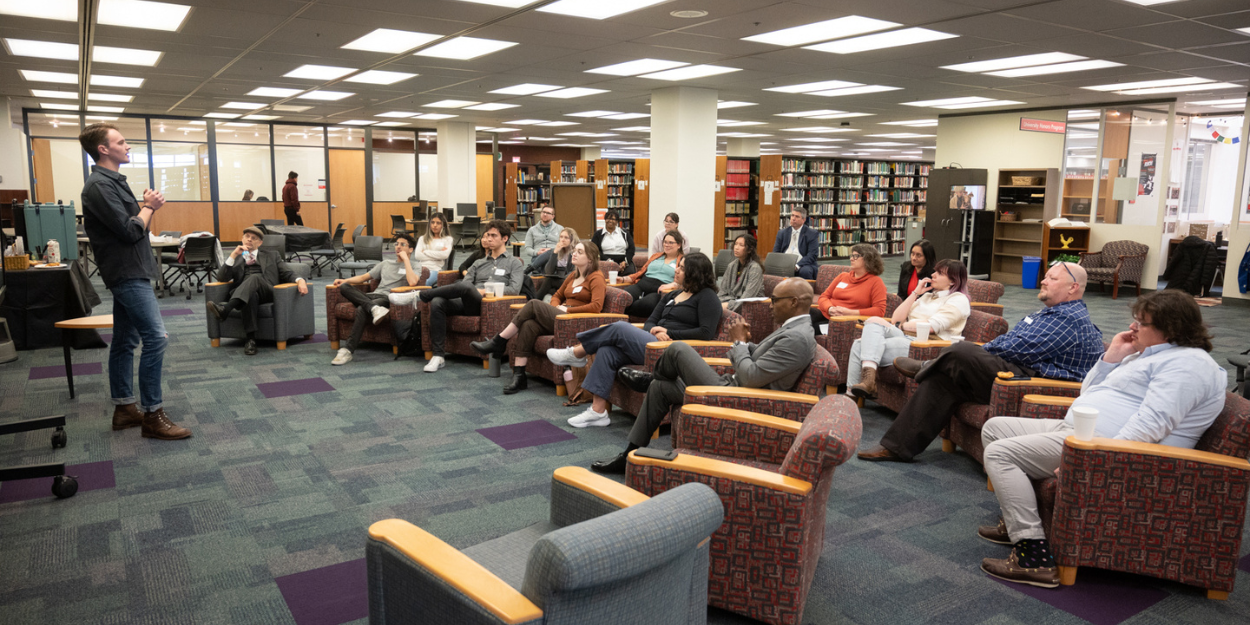
\includegraphics[width=1\linewidth,height=\textheight,keepaspectratio]{images/lovejoy.png}
\caption{Interior shot of Lovejoy Library.}
\end{figure}

\subsection*{Comprehensive Research Resources}\label{comprehensive-research-resources}
\addcontentsline{toc}{subsection}{Comprehensive Research Resources}

Lovejoy Library provides access to an extensive collection of resources, both physical and digital:

\begin{itemize}
\tightlist
\item
  \textbf{Books and Journals}: A vast array of print and electronic volumes spanning diverse disciplines.
\item
  \textbf{Specialized Databases}: Resources such as JSTOR, ProQuest, and EBSCOhost provide access to peer-reviewed articles and other scholarly materials. These databases support keyword searches, author lookups, and advanced filters to streamline research.
\item
  \textbf{Multimedia and Government Documents}: Supplementary resources that enhance interdisciplinary studies.
\end{itemize}

Using the \textbf{online catalog}, students can search for books, articles, and other materials, place holds on physical resources, and access digital content. Filters for subject, date, or resource type simplify the search process.

\subsection*{Personalized Support and Expert Guidance}\label{personalized-support-and-expert-guidance}
\addcontentsline{toc}{subsection}{Personalized Support and Expert Guidance}

The library's staff of skilled librarians provides personalized assistance to help students refine research topics, navigate databases, and develop effective strategies for sourcing credible information:

\begin{itemize}
\tightlist
\item
  \textbf{One-on-One Consultations}: Schedule sessions with librarians for tailored research support.
\item
  \textbf{Ask-A-Librarian Service}: Get quick answers via chat, email, or phone.
\item
  \textbf{Workshops and Tutorials}: Learn about database navigation, citation management, and avoiding plagiarism through interactive sessions.
\end{itemize}

\subsection*{Study and Collaboration Spaces}\label{study-and-collaboration-spaces}
\addcontentsline{toc}{subsection}{Study and Collaboration Spaces}

Lovejoy Library is designed to support a variety of study needs:

\begin{itemize}
\tightlist
\item
  \textbf{Quiet Study Areas}: Individual workspaces free from distractions.
\item
  \textbf{Group Study Rooms}: Collaborative spaces equipped for team projects.
\item
  \textbf{Technology Access}: Computer labs with software like RStudio, Tableau, and Adobe Creative Suite, along with printers and scanners.
\end{itemize}

\subsection*{Citation and Academic Integrity Tools}\label{citation-and-academic-integrity-tools}
\addcontentsline{toc}{subsection}{Citation and Academic Integrity Tools}

Proper citation is critical for maintaining academic integrity. Lovejoy Library provides:

\begin{itemize}
\tightlist
\item
  \textbf{Citation Management Tools}: Support for Zotero and EndNote to organize references efficiently.
\item
  \textbf{Workshops on Academic Integrity}: Sessions addressing plagiarism and proper citation practices.
\end{itemize}

\begin{figure}
\centering
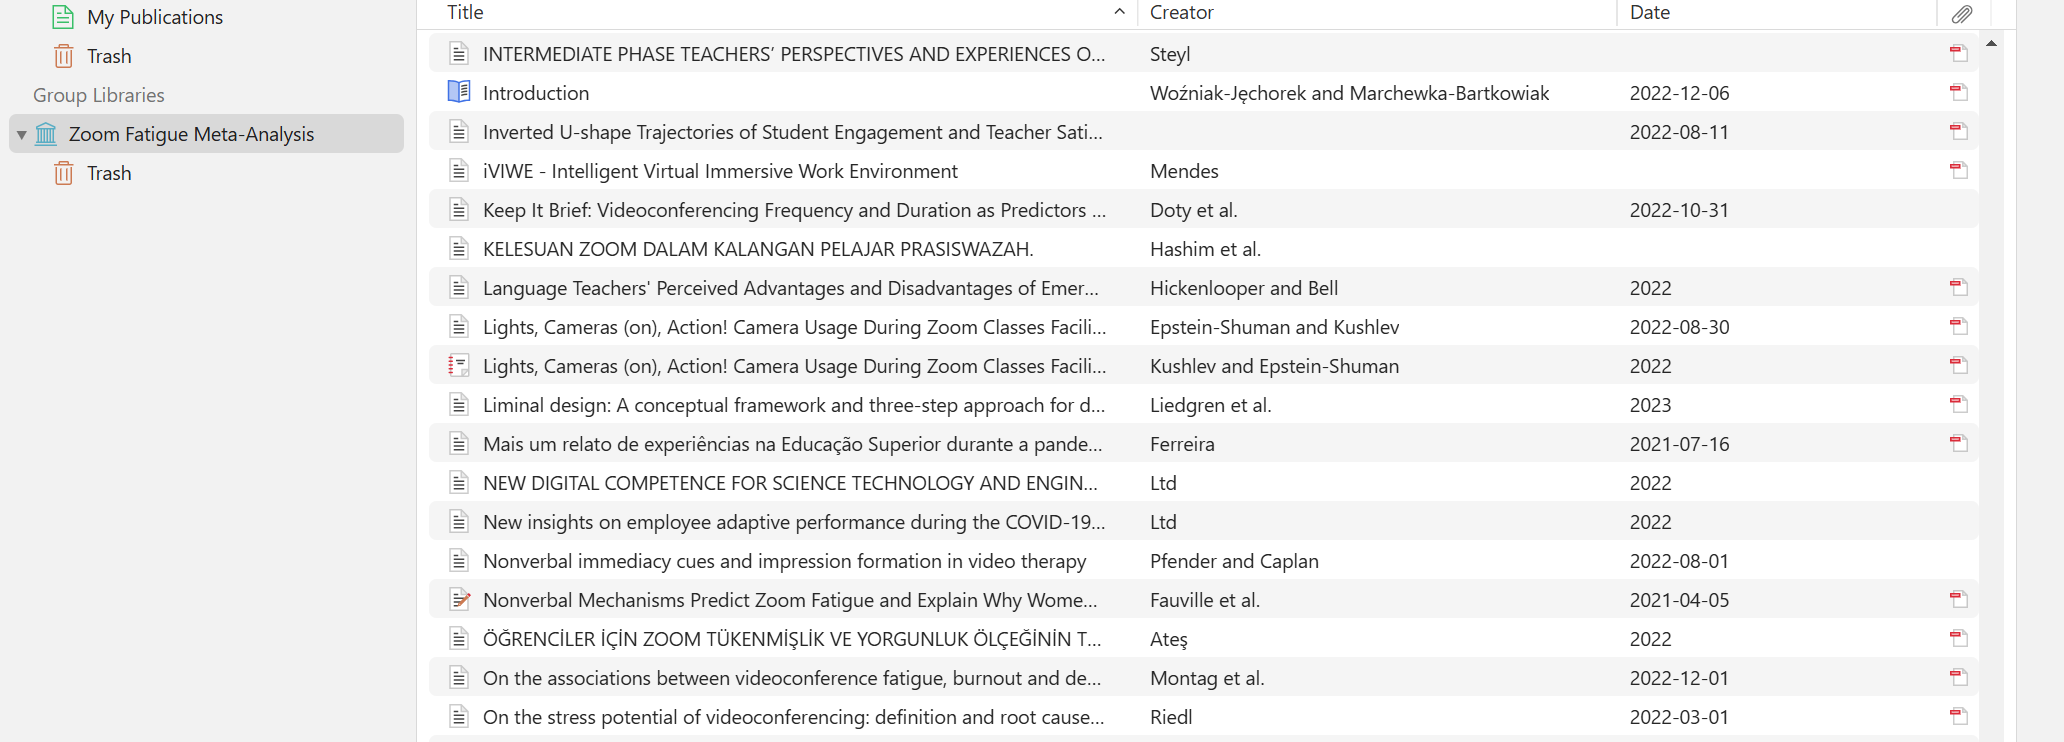
\includegraphics[width=1\linewidth,height=\textheight,keepaspectratio]{images/zotero-library.png}
\caption{Screen capture of a Zotero library.}
\end{figure}

\subsection*{Why Engage with Lovejoy Library?}\label{why-engage-with-lovejoy-library}
\addcontentsline{toc}{subsection}{Why Engage with Lovejoy Library?}

Engaging with the resources and expertise at Lovejoy Library can significantly enhance your academic journey:

\begin{itemize}
\tightlist
\item
  Gain access to credible sources.
\item
  Develop research and critical thinking skills.
\item
  Create a strong foundation for future academic and professional success.
\end{itemize}

By utilizing these resources, students can transform academic challenges into opportunities for growth and discovery.

\section{SIUE Writing Center}\label{siue-writing-center}

The Writing Center at Southern Illinois University Edwardsville (SIUE) is a cornerstone for developing strong academic writing skills. Offering personalized support and comprehensive resources, the Writing Center empowers students to excel in their writing projects while building confidence and independence as writers.

\subsection*{Personalized Tutoring Sessions}\label{personalized-tutoring-sessions}
\addcontentsline{toc}{subsection}{Personalized Tutoring Sessions}

The Writing Center provides \textbf{one-on-one tutoring sessions} to address specific writing challenges:

\begin{itemize}
\tightlist
\item
  \textbf{Brainstorming Ideas}: Assistance with generating topics and developing thesis statements.
\item
  \textbf{Drafting and Organization}: Support for structuring arguments and creating cohesive narratives.
\item
  \textbf{Grammar and Style}: Guidance on sentence structure, clarity, and overall style.
\end{itemize}

\begin{figure}
\centering
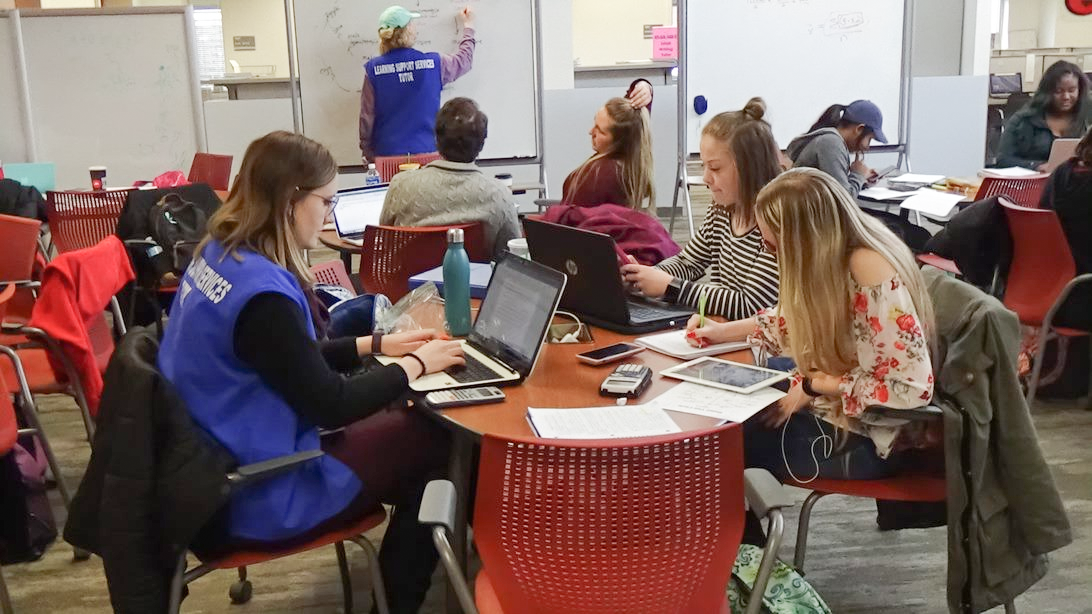
\includegraphics[width=1\linewidth,height=\textheight,keepaspectratio]{images/tutoring.png}
\caption{Tutoring at the Writing Center.}
\end{figure}

Tutors work collaboratively with students to identify areas for improvement, offering feedback that fosters skill development rather than merely correcting errors.

\subsection*{Navigating Academic Formatting and Citations}\label{navigating-academic-formatting-and-citations}
\addcontentsline{toc}{subsection}{Navigating Academic Formatting and Citations}

For research projects requiring specific style guidelines, the Writing Center offers expertise in:

\begin{itemize}
\tightlist
\item
  \textbf{APA, MLA, and Chicago Style}: Assistance with proper formatting, citation practices, and bibliographies.
\item
  \textbf{Avoiding Plagiarism}: Guidance on integrating sources responsibly and maintaining academic integrity.
\end{itemize}

\subsection*{Workshops and Online Resources}\label{workshops-and-online-resources}
\addcontentsline{toc}{subsection}{Workshops and Online Resources}

The Writing Center also hosts workshops and provides online tools to support self-directed learning:

\begin{itemize}
\tightlist
\item
  \textbf{Workshops}: Topics include structuring research papers, integrating evidence, and developing revision strategies.
\item
  \textbf{Online Resources}: Handouts, video tutorials, and guides on writing fundamentals, accessible through the Writing Center's website.
\end{itemize}

\subsection*{Appointment Options and Procedures}\label{appointment-options-and-procedures}
\addcontentsline{toc}{subsection}{Appointment Options and Procedures}

Students can schedule tutoring sessions in various formats:

\begin{enumerate}
\def\labelenumi{\arabic{enumi}.}
\tightlist
\item
  \textbf{In-Person Tutoring}: Traditional face-to-face sessions at the Writing Center.
\item
  \textbf{Online Tutoring}: Real-time video sessions with a tutor, focusing on specific areas of concern.
\item
  \textbf{e-Tutoring}: Submit your paper via email and receive asynchronous feedback with comments and suggestions.
\end{enumerate}

To schedule a session:

\begin{itemize}
\tightlist
\item
  Visit \href{https://siue.mywconline.com/}{siue.mywconline.com}.
\item
  Provide details about your assignment and areas of concern.
\item
  Choose your preferred tutoring format.
\end{itemize}

\textbf{Session Guidelines}:

\begin{itemize}
\tightlist
\item
  Sessions are limited to 30 minutes.
\item
  Students may schedule one session per day and up to two sessions per week.
\end{itemize}

\subsection*{Empowering Confident Writers}\label{empowering-confident-writers}
\addcontentsline{toc}{subsection}{Empowering Confident Writers}

The Writing Center emphasizes teaching students how to identify and address their own writing challenges, fostering long-term growth. By engaging with its resources and services, students not only improve individual assignments but also develop skills that will serve them throughout their academic and professional careers.

\section{Institutional Review Board (IRB)}\label{institutional-review-board-irb}

The Institutional Review Board (IRB) at Southern Illinois University Edwardsville (SIUE) plays an essential role in ensuring that research involving human participants is conducted ethically and in compliance with federal regulations and institutional policies. For students and new researchers, navigating the IRB process may initially appear complex, but it is an invaluable component of conducting responsible and credible research. Understanding the IRB's purpose, processes, and requirements will not only help you meet ethical and regulatory standards but also enhance the quality and integrity of your work.

\subsection*{The Role and Principles of the IRB}\label{the-role-and-principles-of-the-irb}
\addcontentsline{toc}{subsection}{The Role and Principles of the IRB}

The IRB is tasked with reviewing research proposals to ensure that studies involving human participants adhere to ethical principles and minimize risks. This oversight is grounded in the principles established by the Belmont Report:

\begin{enumerate}
\def\labelenumi{\arabic{enumi}.}
\tightlist
\item
  \textbf{Respect for Persons}: Researchers must uphold participants' autonomy and ensure informed consent. This includes providing clear, accessible information about the study's purpose, procedures, and potential risks and benefits.
\item
  \textbf{Beneficence}: Studies must be designed to maximize benefits and minimize harm to participants, ensuring their well-being is prioritized throughout the research process.
\item
  \textbf{Justice}: Researchers must ensure the equitable selection of participants, avoiding exploitation of vulnerable groups and ensuring fair distribution of risks and benefits.
\end{enumerate}

\subsection*{Navigating the IRB Process}\label{navigating-the-irb-process}
\addcontentsline{toc}{subsection}{Navigating the IRB Process}

Before initiating any study involving human participants, researchers must submit their project for IRB review. The process involves several key steps:

\subsubsection*{Step 1: Screening and Submission}\label{step-1-screening-and-submission}
\addcontentsline{toc}{subsubsection}{Step 1: Screening and Submission}

Determine whether your project qualifies as human subjects research (HSR) and requires IRB approval. SIUE provides a screening tool within the Kuali electronic protocol system to help researchers make this determination. Common activities requiring IRB review include surveys, interviews, focus groups, and experiments involving human data. Even if your study may qualify for exempt status (e.g., anonymous surveys), the IRB must still review and approve the protocol.

\begin{itemize}
\tightlist
\item
  \textbf{Review Timelines}:

  \begin{itemize}
  \tightlist
  \item
    Exempt Review: 1--3 weeks
  \item
    Expedited Review: 3--6 weeks
  \item
    Full Board Review: 4--8 weeks or longer (reviewed during monthly meetings)
  \end{itemize}
\end{itemize}

For full board reviews, submit your protocol at least two weeks before the second Wednesday of the month to meet the monthly meeting deadline.

\subsubsection*{Step 2: CITI Certification}\label{step-2-citi-certification}
\addcontentsline{toc}{subsubsection}{Step 2: CITI Certification}

All researchers involved in the study must complete the Collaborative Institutional Training Initiative (CITI) certification before IRB approval. This training ensures researchers understand ethical standards and best practices for working with human participants. Courses include:

\begin{itemize}
\tightlist
\item
  \textbf{IRB Social Behavioral Student}
\item
  \textbf{IRB Social Behavioral Faculty}
\item
  \textbf{Biomedical Researcher}
\item
  \textbf{IRB Member}
\end{itemize}

\begin{figure}
\centering

\includegraphics[width=1\linewidth,height=\textheight,keepaspectratio]{images/irb-cert.png}
\caption{Dr.~Leith's IRB Certification.}
\end{figure}

CITI training provides critical insights into informed consent, confidentiality, and managing participant risks, equipping you to design ethically sound research.

\subsubsection*{Step 3: Preparing and Submitting Your Protocol}\label{step-3-preparing-and-submitting-your-protocol}
\addcontentsline{toc}{subsubsection}{Step 3: Preparing and Submitting Your Protocol}

Log into the \href{https://siue.kuali.co/protocols}{Kuali Online IRB Protocol System} to create and submit your protocol. Your submission should include:

\begin{itemize}
\tightlist
\item
  A detailed study description outlining its purpose, methodology, and expected outcomes
\item
  Informed consent forms with clear, participant-friendly language
\item
  Recruitment materials, surveys, interview guides, or other relevant documents
\end{itemize}

\begin{figure}
\centering
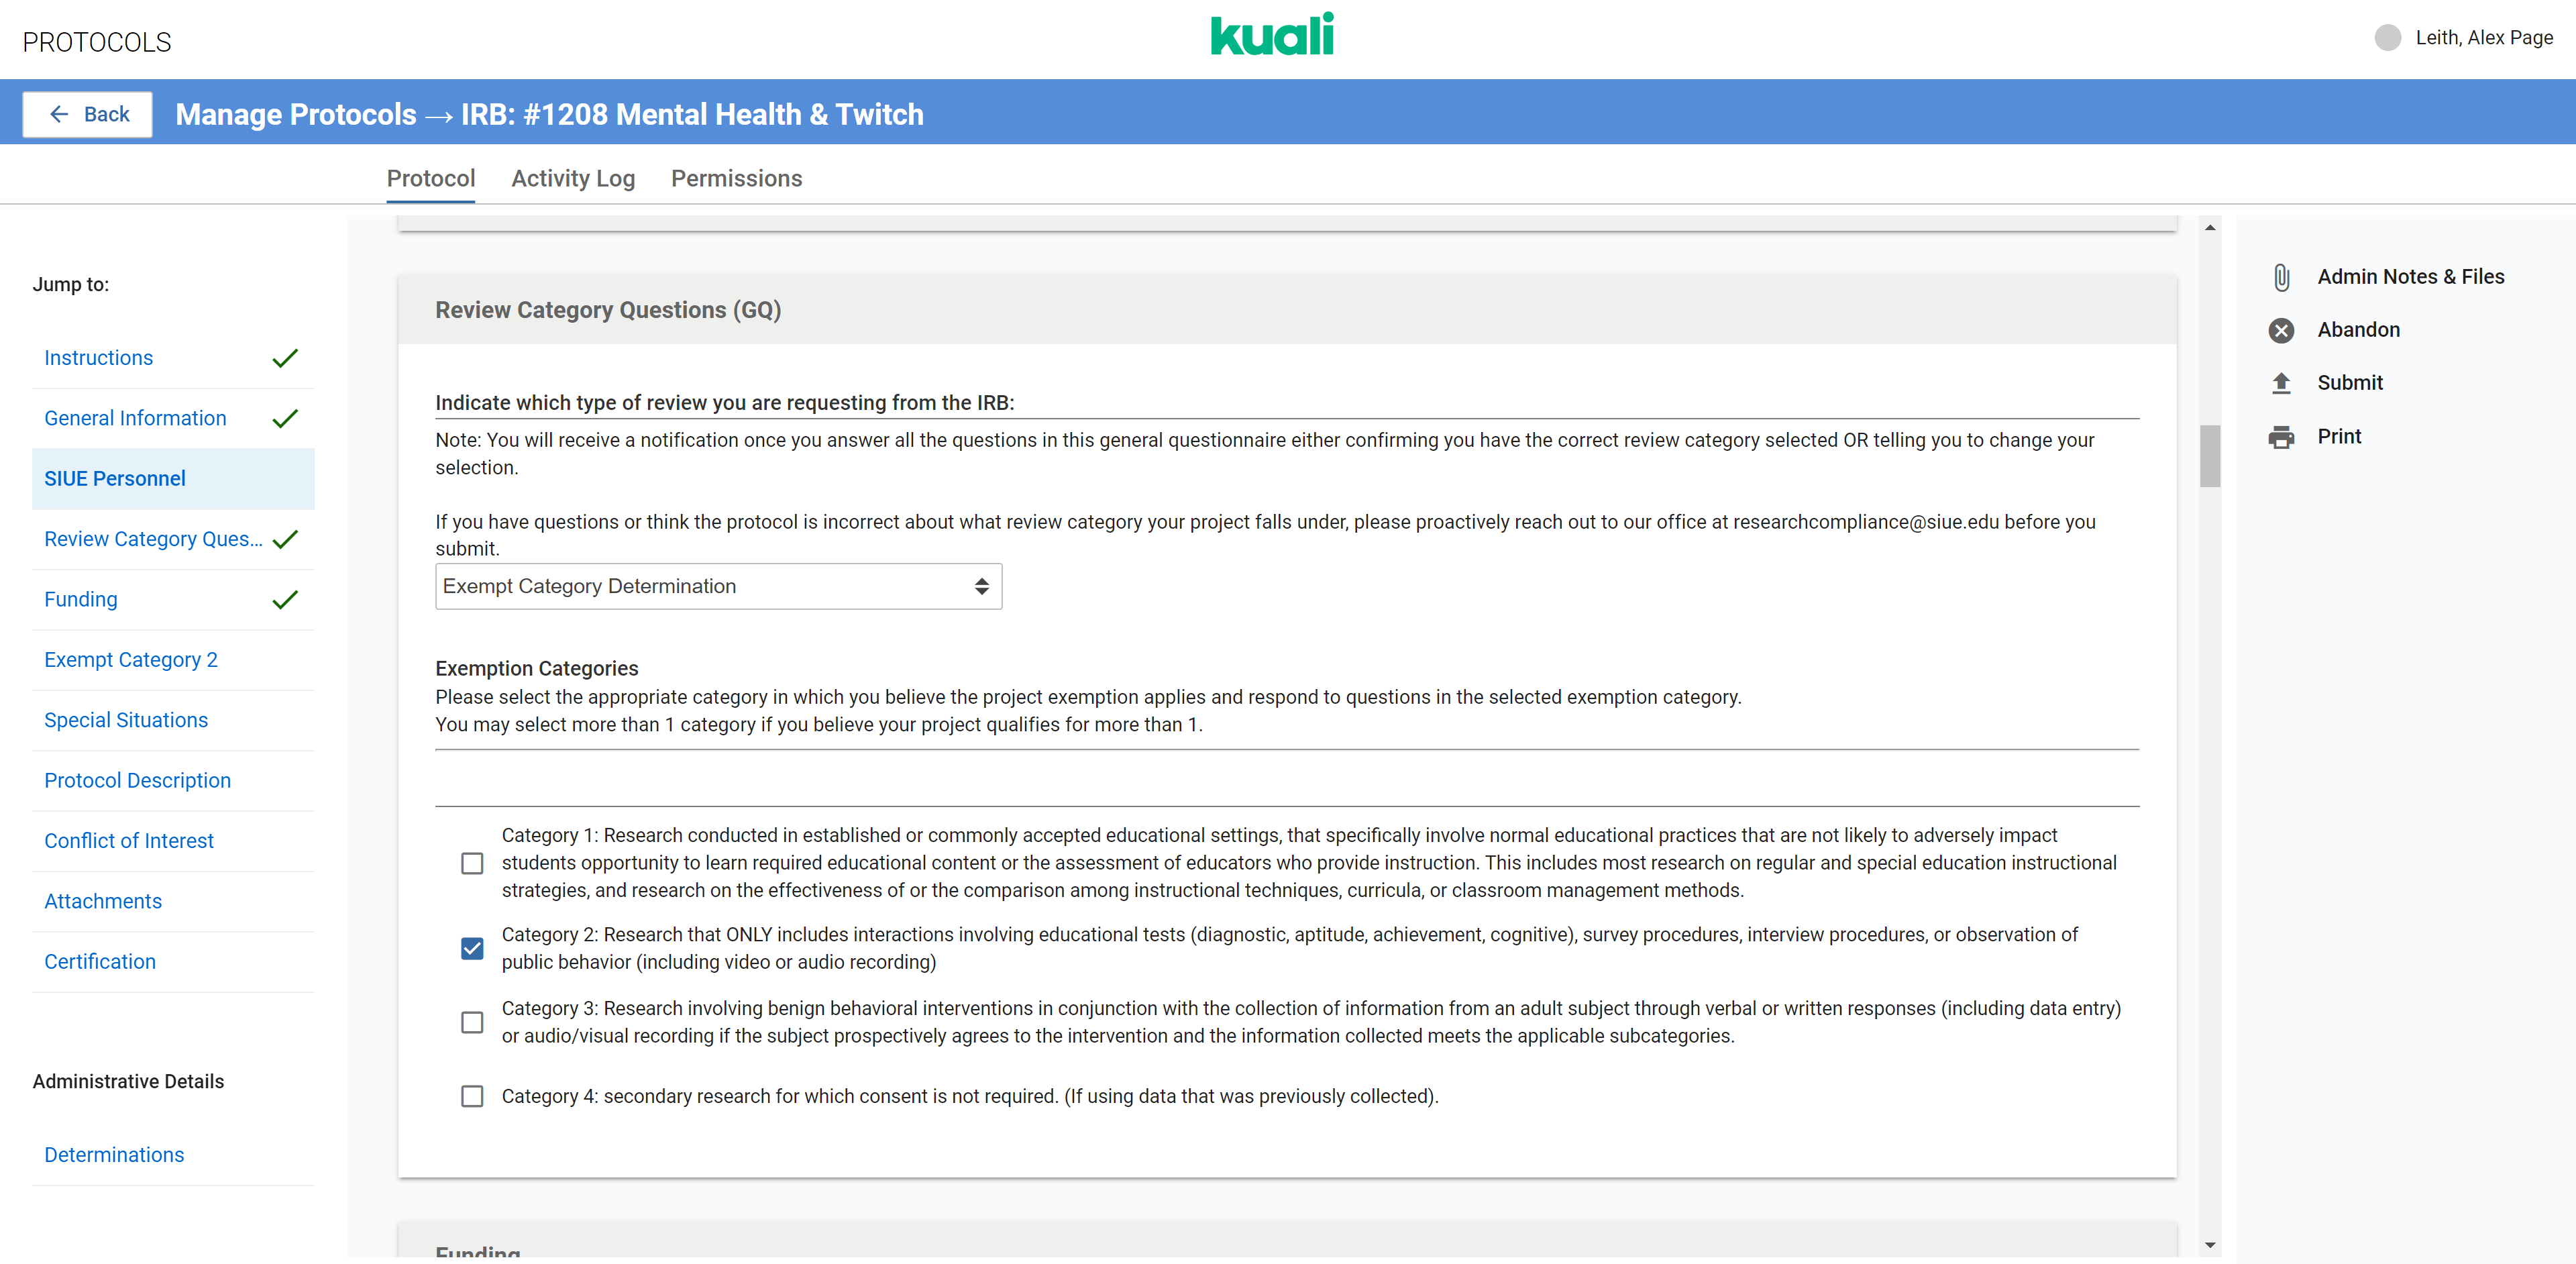
\includegraphics[width=1\linewidth,height=\textheight,keepaspectratio]{images/kuali-exempt.png}
\caption{Kuali section for select exempt status.}
\end{figure}

For guidance, use the available \href{https://www.siue.edu/its/training/KRProtocols/story_html5.html}{online tutorial} and \href{https://www.siue.edu/compliance/human-subjects/pdf/IRBProtocolGuidance.pdf}{IRB Protocol Guide}. Faculty may direct students to the \href{https://siue-sbx.kuali.co/protocols}{SandBox Practice Site} to familiarize themselves with the system before submitting a live protocol.

\subsubsection*{Step 4: Insurance for Student-Initiated Research}\label{step-4-insurance-for-student-initiated-research}
\addcontentsline{toc}{subsubsection}{Step 4: Insurance for Student-Initiated Research}

If your study is not part of a course or degree requirement, you may need to obtain research insurance. The SIU Risk Management Office provides details on \href{http://siusystem.edu/risk-management/insurancereq.shtml}{required coverage}. Proof of insurance must be submitted before protocol approval.

\subsubsection*{Step 5: Post-Approval Responsibilities}\label{step-5-post-approval-responsibilities}
\addcontentsline{toc}{subsubsection}{Step 5: Post-Approval Responsibilities}

Once your protocol is approved, it is essential to adhere to the approved procedures and promptly report any changes, adverse events, or project completion. Use the Kuali system to:

\begin{enumerate}
\def\labelenumi{\arabic{enumi}.}
\tightlist
\item
  \textbf{Amend Protocols}: Submit changes to your study and await IRB approval before implementing them.
\item
  \textbf{Submit Reports}: Provide annual progress reports or completion reports as instructed by the IRB.
\end{enumerate}

\subsubsection*{Step 6: Reporting Adverse Events}\label{step-6-reporting-adverse-events}
\addcontentsline{toc}{subsubsection}{Step 6: Reporting Adverse Events}

Any unanticipated problems or adverse events must be reported to the IRB immediately by contacting \href{mailto:Researchcompliance@siue.edu}{researchcompliance@siue.edu} or calling 618-650-3010. Timely reporting ensures participant safety and compliance with federal regulations.

\subsection*{Levels of IRB Review}\label{levels-of-irb-review}
\addcontentsline{toc}{subsection}{Levels of IRB Review}

The IRB provides three levels of review based on the risk level and study complexity:

\begin{enumerate}
\def\labelenumi{\arabic{enumi}.}
\tightlist
\item
  \textbf{Exempt Review}: For minimal-risk studies, such as anonymous surveys. These receive a quicker review process.
\item
  \textbf{Expedited Review}: For research involving minimal risk but requiring more thorough review, such as non-anonymous interviews.
\item
  \textbf{Full Board Review}: For studies involving greater risks, such as sensitive topics or vulnerable populations. These reviews are conducted during monthly meetings and require detailed scrutiny.
\end{enumerate}

\subsection*{Why Engage with the IRB?}\label{why-engage-with-the-irb}
\addcontentsline{toc}{subsection}{Why Engage with the IRB?}

While the IRB process may seem daunting, it provides several benefits:

\begin{itemize}
\tightlist
\item
  \textbf{Strengthens Research Design}: IRB feedback helps refine your methodology, ensuring ethical rigor and clear protocols.
\item
  \textbf{Builds Ethical Awareness}: Engaging with the IRB process prepares you to conduct responsible research throughout your career.
\item
  \textbf{Fosters Credibility}: Ethical compliance enhances the integrity and impact of your findings, fostering trust within the academic community and beyond.
\end{itemize}

\subsection*{Resources and Support}\label{resources-and-support}
\addcontentsline{toc}{subsection}{Resources and Support}

SIUE's IRB offers extensive resources to guide researchers:

\begin{itemize}
\tightlist
\item
  \textbf{Workshops and Tutorials}: Gain hands-on training to navigate the IRB process confidently.
\item
  \textbf{Templates and Tools}: Access standardized forms for informed consent, recruitment, and study design.
\item
  \textbf{Consultations}: Schedule one-on-one meetings with IRB staff to address specific questions or concerns.
\end{itemize}

By understanding and engaging with the IRB process, you ensure that your research meets the highest ethical standards, contributing to knowledge advancement while safeguarding the well-being of participants. Ethical research practices are not just a requirement---they are a commitment to integrity and respect for the individuals and communities involved in your studies.

\section{Office of Research and Projects (ORP)}\label{office-of-research-and-projects-orp}

The Office of Research and Projects (ORP) at Southern Illinois University Edwardsville (SIUE) is a vital resource for fostering and supporting research, scholarship, and creative activities across the university. For students, faculty, and staff, the ORP serves as a comprehensive hub for navigating the complexities of research funding, compliance, and project management. By engaging with the ORP, researchers gain access to a wide range of resources designed to enhance their work's quality, impact, and ethical rigor.

\subsection*{Research Funding and Proposal Development}\label{research-funding-and-proposal-development}
\addcontentsline{toc}{subsection}{Research Funding and Proposal Development}

A primary role of the ORP is to assist researchers in securing funding for their projects. Whether you are applying for internal grants at SIUE or seeking external funding from organizations like the National Science Foundation (NSF), the ORP provides personalized support to help you identify opportunities that align with your research interests. Services include:

\begin{itemize}
\tightlist
\item
  \textbf{Funding Opportunity Identification}: Access tools and databases to find grants that match your project's goals.
\item
  \textbf{Proposal Development Support}: Participate in workshops or schedule one-on-one consultations to craft competitive proposals, write persuasive narratives, and align your objectives with the priorities of funding agencies.
\item
  \textbf{Internal Funding Programs}: Apply for internal awards that support both faculty and student research initiatives.
\end{itemize}

These services are particularly valuable for new researchers, offering step-by-step guidance through the grant application process and equipping them with skills that extend beyond academia.

\subsection*{Ensuring Compliance and Ethical Research}\label{ensuring-compliance-and-ethical-research}
\addcontentsline{toc}{subsection}{Ensuring Compliance and Ethical Research}

The ORP plays a central role in ensuring that all research activities adhere to institutional policies, federal regulations, and ethical guidelines. Key areas of compliance include:

\begin{itemize}
\tightlist
\item
  \textbf{Human Subjects Research}: Collaborating with the Institutional Review Board (IRB) to review and approve projects involving surveys, interviews, or other interactions with human participants.
\item
  \textbf{Animal Research}: Providing oversight and guidance for studies involving animals to ensure adherence to ethical standards.
\item
  \textbf{Hazardous Materials and Specialized Facilities}: Offering support to manage projects requiring the use of hazardous materials, specialized labs, or sensitive data.
\end{itemize}

\begin{figure}
\centering

\includegraphics[width=1\linewidth,height=\textheight,keepaspectratio]{images/orp-preaward.png}
\caption{Pre-award resources available through SIUE's ORP.}
\end{figure}

The ORP's \textbf{Compliance Section} ensures that research is conducted with integrity, balancing the interests of the university, researchers, participants, and funding agencies. For more details, consult the \href{https://www.siue.edu/compliance/}{Compliance Website}.

\subsection*{Project Management and Post-Award Support}\label{project-management-and-post-award-support}
\addcontentsline{toc}{subsection}{Project Management and Post-Award Support}

Securing funding is only the first step in a successful research project. Managing the financial, logistical, and reporting aspects of a grant can be challenging, particularly for those new to research. The ORP offers:

\begin{itemize}
\tightlist
\item
  \textbf{Pre-Award Support}: Assistance with budget development, proposal submission, and navigating sponsor guidelines through tools like \textbf{Kuali Research}.
\item
  \textbf{Post-Award Management}: Guidance on tracking expenditures, fulfilling reporting requirements, and ensuring compliance with sponsor mandates.
\end{itemize}

By simplifying administrative tasks, the ORP allows researchers to focus on the intellectual and creative aspects of their work, ensuring projects remain on track and meet all obligations.

\subsection*{Building a Collaborative Research Environment}\label{building-a-collaborative-research-environment}
\addcontentsline{toc}{subsection}{Building a Collaborative Research Environment}

The ORP actively fosters interdisciplinary collaboration among researchers at SIUE, creating opportunities to share ideas and build partnerships. Through networking events, research symposia, and seminars, the ORP provides a platform for researchers across disciplines to connect and tackle complex challenges together. For students, these events offer valuable exposure to innovative methodologies, diverse perspectives, and potential collaborators.

\subsection*{Student-Focused Resources}\label{student-focused-resources}
\addcontentsline{toc}{subsection}{Student-Focused Resources}

Recognizing the importance of nurturing new researchers, the ORP offers tailored resources for students:

\begin{itemize}
\tightlist
\item
  \textbf{Workshops and Training}: Learn critical skills such as proposal writing, research ethics, and project management in hands-on sessions.
\item
  \textbf{Online Resources}: Access templates, examples of successful proposals, and guides for navigating funding databases through the ORP website.
\item
  \textbf{Practice Platforms}: Use tools like the \textbf{Kuali Build SandBox Site} to simulate protocol creation and learn the system before submitting live applications.
\end{itemize}

By providing these resources, the ORP demystifies the research process and builds students' confidence, enabling them to engage in meaningful scholarship.

\subsection*{Tools and Resources Available Through the ORP}\label{tools-and-resources-available-through-the-orp}
\addcontentsline{toc}{subsection}{Tools and Resources Available Through the ORP}

The ORP provides access to a range of tools designed to streamline research administration:

\begin{itemize}
\tightlist
\item
  \textbf{Kuali Research}: A comprehensive platform for submitting disclosures, managing sub-awards, and tracking progress.
\item
  \textbf{Kuali Build}: An electronic system for routing and submitting internal funding applications and forms.
\item
  \textbf{ORP Quick Reference Guide}: A resource for developing budgets, creating cover sheets, and navigating application requirements.
\end{itemize}

\subsection*{The Role of the ORP in Academic and Professional Growth}\label{the-role-of-the-orp-in-academic-and-professional-growth}
\addcontentsline{toc}{subsection}{The Role of the ORP in Academic and Professional Growth}

The ORP is more than an administrative office---it is a partner in your academic and professional journey. By engaging with its services early, students and faculty can:

\begin{itemize}
\tightlist
\item
  \textbf{Enhance Research Quality}: Leverage expert guidance to refine proposals and methodologies.
\item
  \textbf{Ensure Ethical Integrity}: Meet the highest standards for compliance and ethical conduct in research.
\item
  \textbf{Expand Opportunities}: Build connections across disciplines, access funding, and develop critical research skills.
\end{itemize}

\subsection*{Balancing Institutional and Researcher Objectives}\label{balancing-institutional-and-researcher-objectives}
\addcontentsline{toc}{subsection}{Balancing Institutional and Researcher Objectives}

The ORP carefully balances the university's mission, the intellectual pursuits of researchers, and the objectives of funding agencies. This approach ensures that research activities are aligned with SIUE's broader goals while empowering individual scholars to pursue innovative and impactful work.

\section{Zotero - Citation Management Made Simple}\label{zotero---citation-management-made-simple}

\textbf{Zotero} is an indispensable tool for managing citations and organizing research at Southern Illinois University Edwardsville (SIUE). This free, user-friendly software simplifies the process of collecting, organizing, and citing sources, making it ideal for students and researchers alike.

\subsection*{Key Features of Zotero}\label{key-features-of-zotero}
\addcontentsline{toc}{subsection}{Key Features of Zotero}

\begin{itemize}
\tightlist
\item
  \textbf{Citation Collection}: Save references from books, articles, and websites with one click.
\item
  \textbf{Integration with Word Processors}: Automatically generate in-text citations and bibliographies in APA, MLA, Chicago, and other styles directly in Microsoft Word, Google Docs, or LibreOffice.
\item
  \textbf{Organization}: Create folders and collections for different projects to keep research materials organized.
\item
  \textbf{Attachments}: Store PDFs, images, and notes alongside your citations.
\end{itemize}

\subsection*{Installation and Usage}\label{installation-and-usage}
\addcontentsline{toc}{subsection}{Installation and Usage}

\begin{itemize}
\tightlist
\item
  \textbf{Zotero Desktop}: Download the latest version from \href{https://www.zotero.org/}{Zotero.org} and install the Zotero Connector plugin for your browser.
\item
  \textbf{Zotero Online}: Access your library anytime by logging into Zotero's website.
\item
  \textbf{Word Processor Plugins}: Use Zotero's plugins to ``cite while you write'' in Word and other platforms.
\end{itemize}

\subsection*{Tutorials and Support}\label{tutorials-and-support}
\addcontentsline{toc}{subsection}{Tutorials and Support}

\begin{itemize}
\tightlist
\item
  SIUE offers workshops and guides to help students maximize Zotero's capabilities. Check out the official \href{https://www.zotero.org/support/quick_start_guide}{Zotero Quick Start Guide} for further details.
\end{itemize}

\textbf{Why Use Zotero?} Zotero streamlines the often-overwhelming task of managing citations, ensuring academic accuracy and saving time, especially for complex research projects.

\section{Information Technology Services (ITS) - Advanced Computing Resources}\label{information-technology-services-its---advanced-computing-resources}

The \textbf{Office of Information Technology Services (ITS)} at SIUE supports advanced research through cutting-edge computing infrastructure and specialized software.

\subsection*{Key Resources and Tools}\label{key-resources-and-tools}
\addcontentsline{toc}{subsection}{Key Resources and Tools}

\begin{itemize}
\tightlist
\item
  \textbf{High-Performance Computing (HPC)}: Access the Slurm Compute Cluster for computational research with both CPU and GPU nodes, optimized for data-intensive projects.
\item
  \textbf{Cyberinfrastructure}:

  \begin{itemize}
  \tightlist
  \item
    10Gb/s connection to Internet2 and the Metropolitan Research and Education Network (MREN).
  \item
    High-performance storage clusters for data-intensive research.
  \item
    OpenStack cluster for virtualized computing needs.
  \end{itemize}
\item
  \textbf{Research Software}: Utilize tools such as RStudio, Python, Tableau, and Adobe Creative Suite for statistical modeling, data visualization, and content creation.
\end{itemize}

\subsection*{Support and Training}\label{support-and-training}
\addcontentsline{toc}{subsection}{Support and Training}

\begin{itemize}
\tightlist
\item
  \textbf{Workshops}: ITS offers training sessions for tools like R, Python, and advanced data visualization software.
\item
  \textbf{Consultation Services}: Tailored guidance for integrating computing resources into research projects.
\end{itemize}

\textbf{Why Leverage ITS?} Whether you're modeling complex systems, analyzing large datasets, or visualizing trends, ITS ensures you have the tools and expertise to succeed.

\section{Undergraduate Research and Creative Activities (URCA)}\label{undergraduate-research-and-creative-activities-urca}

The \textbf{Undergraduate Research and Creative Activities (URCA)} program provides students at SIUE with opportunities to engage in hands-on research and creative projects under faculty mentorship.

\subsection*{Types of URCA Opportunities}\label{types-of-urca-opportunities}
\addcontentsline{toc}{subsection}{Types of URCA Opportunities}

\begin{enumerate}
\def\labelenumi{\arabic{enumi}.}
\tightlist
\item
  \textbf{URCA Assistants}:

  \begin{itemize}
  \tightlist
  \item
    Work with faculty on research or creative projects for 6--9 hours per week.
  \item
    Eligible for a \$750 semester award or academic credit.
  \end{itemize}
\item
  \textbf{URCA Associates}:

  \begin{itemize}
  \tightlist
  \item
    Conduct independent research with faculty supervision.
  \item
    Present findings at conferences or exhibitions.
  \end{itemize}
\end{enumerate}

\subsection*{Benefits of Participation}\label{benefits-of-participation}
\addcontentsline{toc}{subsection}{Benefits of Participation}

\begin{itemize}
\tightlist
\item
  Gain practical experience in research and creative processes.
\item
  Build professional relationships with mentors and peers.
\item
  Strengthen critical thinking, communication, and data analysis skills.
\item
  Enhance your résumé or graduate school applications.
\end{itemize}

\textbf{How to Get Involved}: Visit the \href{https://www.siue.edu/urca/}{URCA Program Website} to explore opportunities and apply.

\section{Interdisciplinary Research and Informatics Scholarship (IRIS)}\label{interdisciplinary-research-and-informatics-scholarship-iris}

The \textbf{IRIS Center} at SIUE fosters innovative, interdisciplinary research at the intersection of technology, humanities, and social sciences.

\subsection*{Mission and Goals}\label{mission-and-goals}
\addcontentsline{toc}{subsection}{Mission and Goals}

\begin{itemize}
\tightlist
\item
  Support digital scholarship through advanced tools and methodologies.
\item
  Facilitate collaboration among faculty and students.
\item
  Promote curricular innovation integrating digital applications.
\item
  Advance community-oriented digital projects.
\end{itemize}

\subsection*{Key Resources}\label{key-resources}
\addcontentsline{toc}{subsection}{Key Resources}

\begin{itemize}
\tightlist
\item
  \textbf{Facilities and Tools}: Access to cutting-edge technology for digital humanities and social sciences research.
\item
  \textbf{Research Consultations}: One-on-one guidance on tool selection, project sustainability, and audience engagement.
\item
  \textbf{The SIM Lab}: Focus on projects related to virtual reality, social media analysis, and human-computer interaction.
\end{itemize}

\textbf{Why Engage with IRIS?} IRIS provides a dynamic environment for exploring emerging trends and technologies, preparing students for future academic and professional challenges.

\chapter{Introduction to Research Papers}\label{introduction-to-research-papers}

\section{Structuring a Research Paper}\label{structuring-a-research-paper}

Writing a research report requires careful organization to effectively communicate the purpose, methods, findings, and conclusions of a study. Each section of a research paper serves a distinct function, guiding the reader through the research process in a logical and structured manner. Understanding the role of each section and how to write them effectively ensures that the paper is clear, coherent, and impactful.

\subsection*{Title}\label{title}
\addcontentsline{toc}{subsection}{Title}

The title of a research paper is the first point of engagement for the reader. It should be \textbf{clear, concise, and informative}, giving a snapshot of the study's focus. A strong title includes key variables or the primary subject of study without being overly lengthy---typically no more than \textbf{12 words}. It should be formatted correctly, \textbf{bold, centered, and double-spaced} on the title page. Capitalization rules apply: \textbf{only the first word and proper nouns are capitalized}, even if a semicolon is used in the title. A well-crafted title ensures the reader understands what to expect, improving discoverability in academic databases.

\subsection*{Abstract}\label{abstract}
\addcontentsline{toc}{subsection}{Abstract}

The \textbf{abstract} is a concise summary of the research paper, typically \textbf{150 to 250 words} long, providing an overview of the study. It is written in \textbf{past tense} and should not contain citations. The abstract must succinctly cover the \textbf{research purpose, methods, key findings, and conclusions}. Since the abstract is often the first---and sometimes only---part of the paper that many readers engage with, clarity and brevity are essential. A well-written abstract enables readers to quickly assess the relevance of the study to their interests and research.

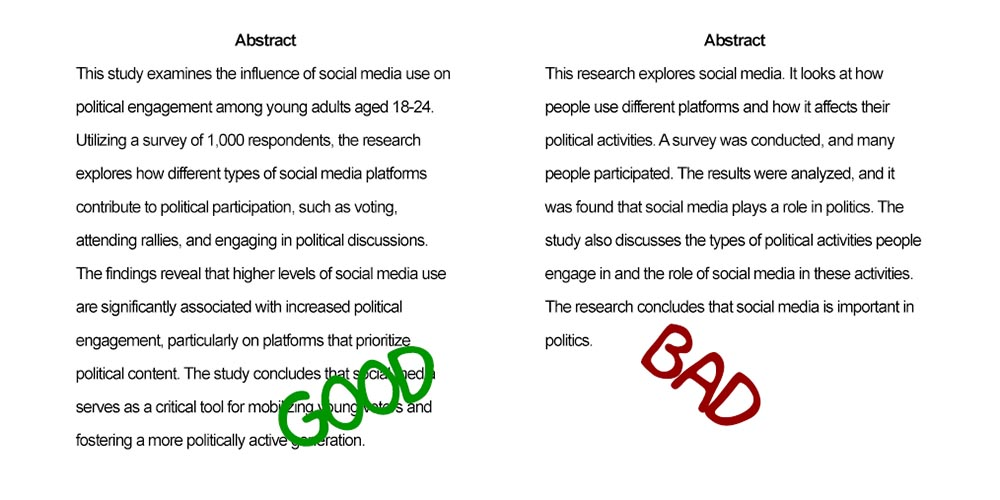
\includegraphics[width=1\linewidth,height=\textheight,keepaspectratio]{images/fig081.jpg}

\subsection*{Introduction}\label{introduction}
\addcontentsline{toc}{subsection}{Introduction}

The \textbf{introduction} provides the foundation for the research paper. It presents the research problem, its significance, and the research question or hypothesis. This section should accomplish the following:

\begin{itemize}
\tightlist
\item
  \textbf{Introduce the topic} and explain its relevance.
\item
  \textbf{Provide background information} and connect it to existing research.
\item
  \textbf{Clearly state the research question or hypothesis.}
\item
  \textbf{Outline the structure} of the paper to help readers navigate the content.
\end{itemize}

A strong introduction engages the reader by linking the study to real-world problems or theoretical debates, setting the stage for the rest of the report.

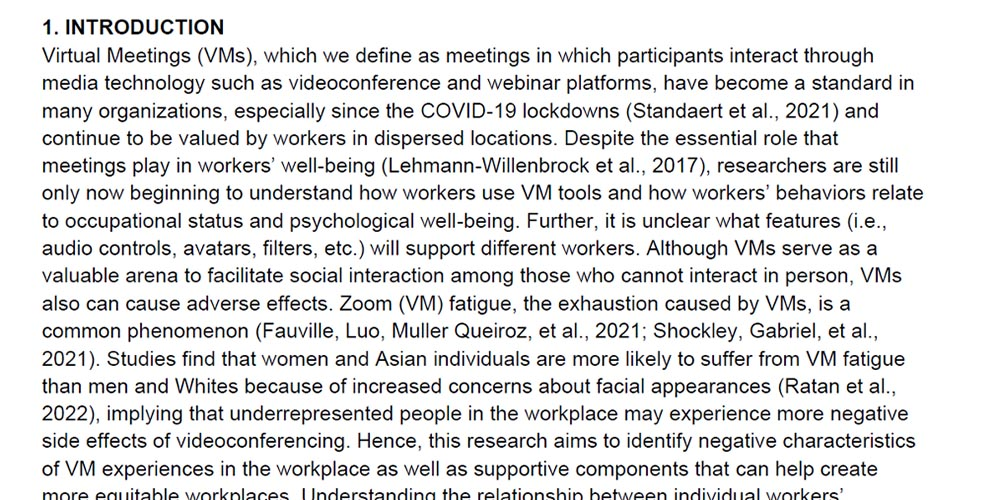
\includegraphics[width=1\linewidth,height=\textheight,keepaspectratio]{images/fig082.jpg}

\subsection*{Literature Review}\label{literature-review}
\addcontentsline{toc}{subsection}{Literature Review}

The \textbf{literature review} contextualizes the research within the existing body of knowledge. Rather than simply summarizing past studies, this section should \textbf{synthesize and critically analyze} prior research, highlighting gaps, contradictions, and areas for further investigation. Key purposes of the literature review include:

\begin{itemize}
\tightlist
\item
  Demonstrating the researcher's knowledge of the field.
\item
  Justifying why the study is needed by identifying gaps in the literature.
\item
  Establishing a theoretical framework for the study.
\item
  Providing a basis for comparing the study's findings with previous research.
\end{itemize}

The literature review should be organized thematically or methodologically, making it easier for readers to follow the connections between different studies and the current research.

\subsection*{Methods}\label{methods}
\addcontentsline{toc}{subsection}{Methods}

The \textbf{methods} section details how the study was conducted, allowing other researchers to replicate the research or assess its validity. It typically includes:

\begin{enumerate}
\def\labelenumi{\arabic{enumi}.}
\tightlist
\item
  \textbf{Participants or Data Sources} -- Describing who or what was studied and how subjects were selected.
\item
  \textbf{Materials or Instruments} -- Identifying tools, surveys, software, or measurement instruments used.
\item
  \textbf{Procedures} -- Outlining the steps taken to collect data.
\item
  \textbf{Data Analysis} -- Explaining how the data was processed and analyzed.
\end{enumerate}

The methods section must be clear, precise, and thorough. It is written in the \textbf{past tense} since it describes completed actions.

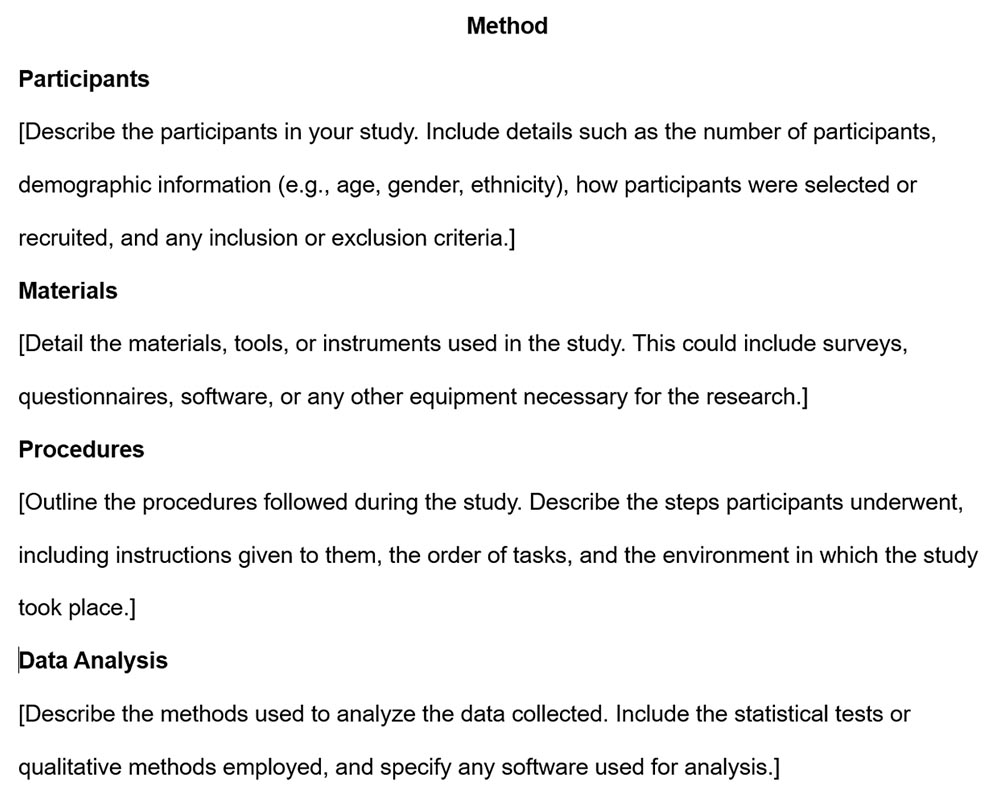
\includegraphics[width=1\linewidth,height=\textheight,keepaspectratio]{images/fig083.jpg}

\subsection*{Results}\label{results}
\addcontentsline{toc}{subsection}{Results}

The \textbf{results} section presents the findings of the study in an objective manner, free from interpretation. It includes:

\begin{itemize}
\tightlist
\item
  \textbf{Descriptive statistics} (e.g., means, standard deviations, frequencies).
\item
  \textbf{Inferential statistics} (e.g., t-tests, ANOVA, regression results).
\item
  \textbf{Tables, graphs, and figures} to enhance clarity.
\end{itemize}

Each result should be clearly labeled and presented logically, often following the structure outlined in the methods section. The results should not include explanations or implications---those belong in the discussion section.

\subsection*{Discussion}\label{discussion}
\addcontentsline{toc}{subsection}{Discussion}

The \textbf{discussion} section interprets the results and relates them back to the research question, hypothesis, and existing literature. This section should:

\begin{enumerate}
\def\labelenumi{\arabic{enumi}.}
\tightlist
\item
  \textbf{Summarize key findings} without simply repeating the results section.
\item
  \textbf{Compare findings to prior research} and theoretical frameworks.
\item
  \textbf{Discuss unexpected results} and possible explanations.
\item
  \textbf{Acknowledge limitations} of the study and their implications.
\item
  \textbf{Suggest directions for future research.}
\end{enumerate}

The discussion provides the critical interpretation of findings, ensuring that the study contributes to ongoing academic conversations.

\subsection*{Conclusion}\label{conclusion}
\addcontentsline{toc}{subsection}{Conclusion}

The \textbf{conclusion} provides a concise summary of the key findings, reinforcing their significance. It should:

\begin{itemize}
\tightlist
\item
  \textbf{Restate the research question and summarize the main findings.}
\item
  \textbf{Explain the broader implications of the study.}
\item
  \textbf{Highlight recommendations for practice, policy, or future research.}
\end{itemize}

A strong conclusion ties everything together without introducing new arguments or data. It leaves the reader with a clear understanding of the study's contribution.

\subsection*{References}\label{references}
\addcontentsline{toc}{subsection}{References}

The \textbf{references} section provides a comprehensive list of all sources cited in the paper, formatted according to the appropriate academic style (e.g., APA, MLA, Chicago). Proper referencing is essential for:

\begin{itemize}
\tightlist
\item
  \textbf{Giving credit to original authors.}
\item
  \textbf{Ensuring academic integrity.}
\item
  \textbf{Allowing readers to locate cited sources.}
\end{itemize}

Students should use reference management tools like \textbf{Zotero, EndNote, or Mendeley} to maintain accurate citations.

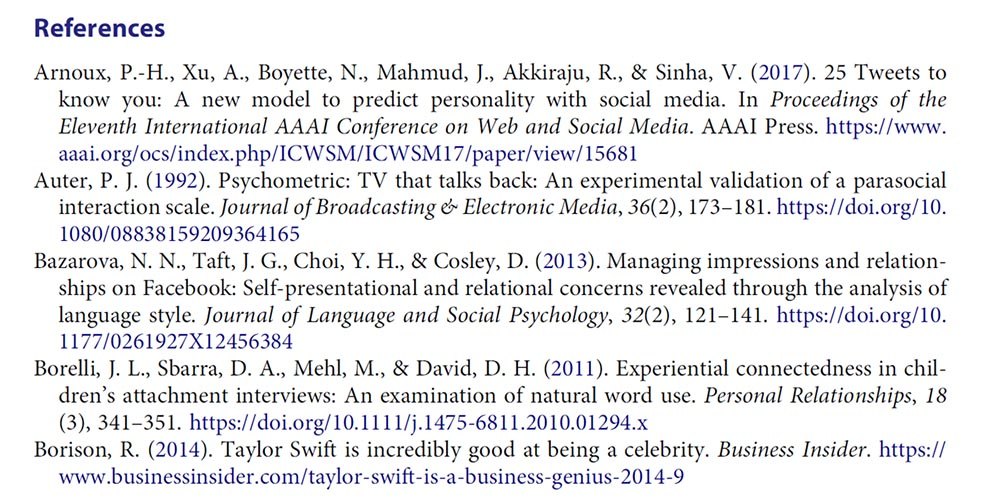
\includegraphics[width=1\linewidth,height=\textheight,keepaspectratio]{images/fig085.jpg}

\subsection*{Appendix}\label{appendix}
\addcontentsline{toc}{subsection}{Appendix}

An \textbf{appendix} contains supplementary materials that are too detailed or extensive for the main body of the paper. These can include:

\begin{itemize}
\tightlist
\item
  Survey instruments.
\item
  Large tables of data.
\item
  Detailed methodological descriptions.
\item
  Additional figures.
\end{itemize}

The appendix should be referenced in the main text when necessary.

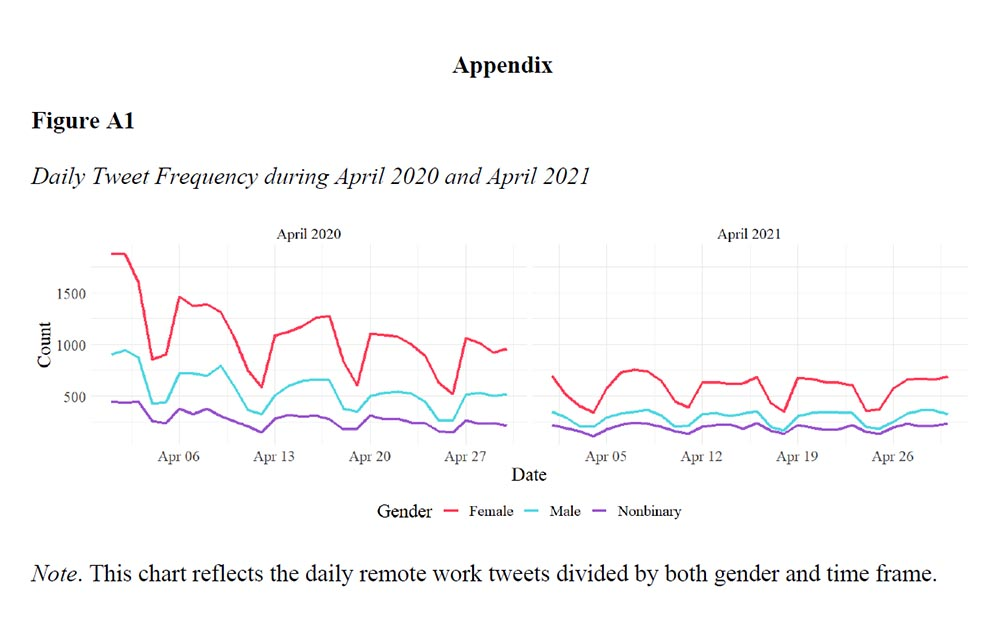
\includegraphics[width=1\linewidth,height=\textheight,keepaspectratio]{images/fig086.jpg}

\subsection*{Relationship Between Sections}\label{relationship-between-sections}
\addcontentsline{toc}{subsection}{Relationship Between Sections}

Each section of a research paper serves a \textbf{distinct but interconnected role}, contributing to the overall coherence of the study:

\begin{enumerate}
\def\labelenumi{\arabic{enumi}.}
\tightlist
\item
  \textbf{The Title and Abstract} capture attention and provide an overview.
\item
  \textbf{The Introduction and Literature Review} establish the context and research justification.
\item
  \textbf{The Methods and Results} document how the study was conducted and what was found.
\item
  \textbf{The Discussion and Conclusion} interpret findings and explain their significance.
\item
  \textbf{References and Appendices} provide support materials and additional resources.
\end{enumerate}

By following this structure, students can ensure their research papers are logically organized, academically rigorous, and effectively communicate their findings.

\subsection*{Examples of Formal Reports}\label{examples-of-formal-reports}
\addcontentsline{toc}{subsection}{Examples of Formal Reports}

\subsubsection*{Academic Examples}\label{academic-examples}
\addcontentsline{toc}{subsubsection}{Academic Examples}

There are many different ways to report research in academia. Some of the most common methods include:

\textbf{Research papers}: Research papers are the most common way to report research in academia. They are typically published in academic journals and are written in a formal style.

\textbf{Conference papers}: Conference papers are presented at academic conferences. They are typically shorter than research papers and are written in a more informal style.

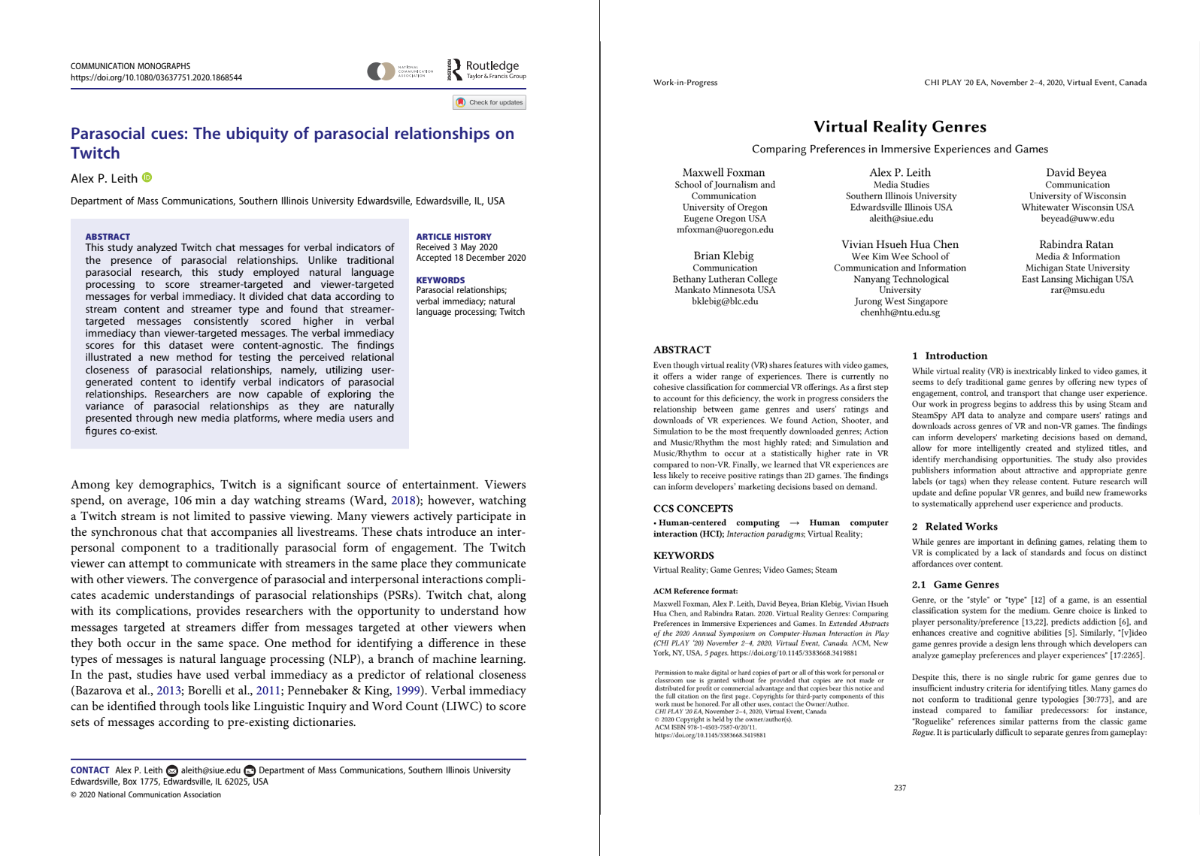
\includegraphics[width=1\linewidth,height=\textheight,keepaspectratio]{images/papers.png}

\textbf{Theses and dissertations}: Theses and dissertations are written by graduate students to complete their degree requirements. They are typically longer and more comprehensive than research papers.

\textbf{Books}: Books are another way to report research. They are typically written by experts in a particular field and can be a good way to communicate research to a wider audience.

\textbf{Reports}: Reports are written for a specific audience, such as a government agency or a business. They are typically shorter than research papers and focus on a specific topic.

\textbf{Presentations}: Presentations are a way to share research with a live audience. They can be given at conferences, workshops, or other events.

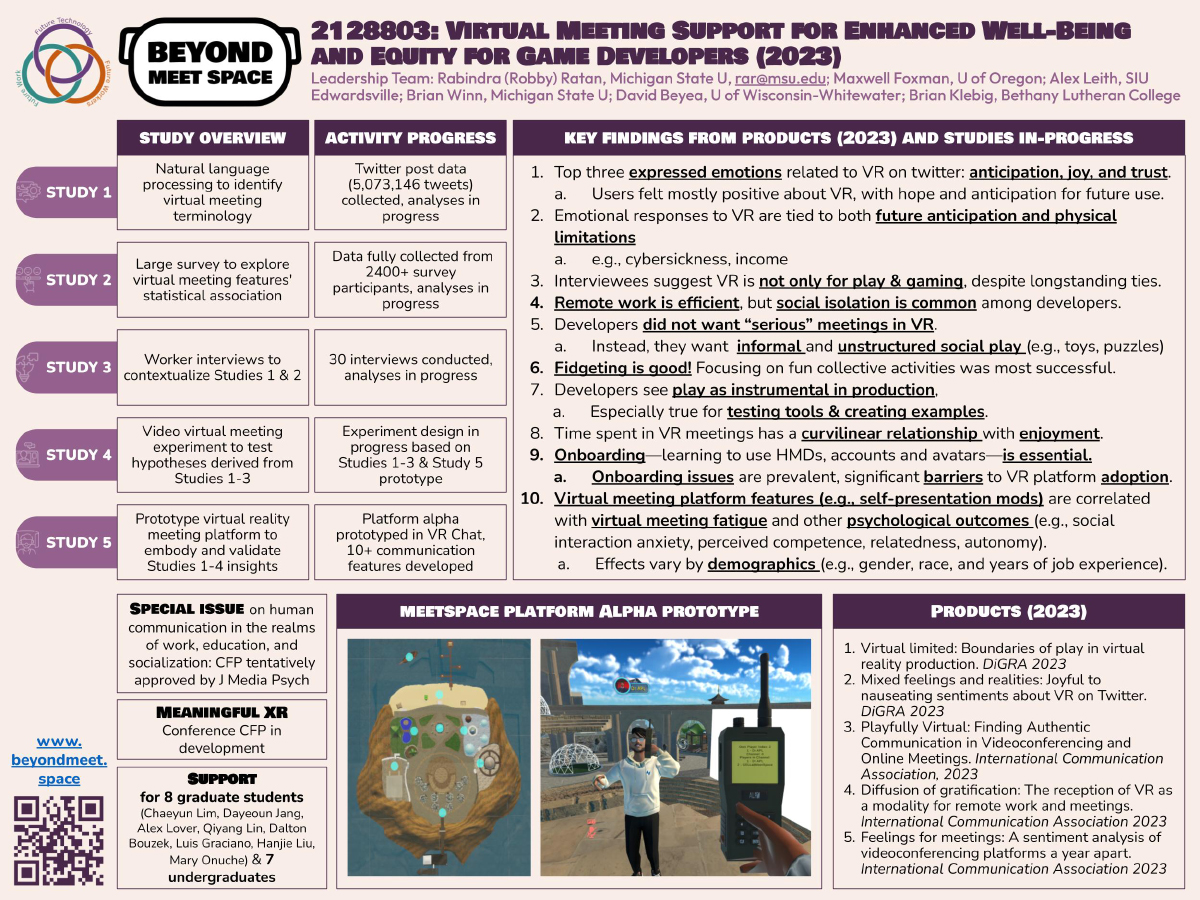
\includegraphics[width=1\linewidth,height=\textheight,keepaspectratio]{images/BMS2023poster.jpg}

\textbf{Blogs and social media}: Blogs and social media can be used to share research with a wider audience. They are a good way to communicate research in a more informal way.

The best way to report research depends on the specific research project and the intended audience. However, all of these methods can be effective ways to communicate research findings and to contribute to the academic community.

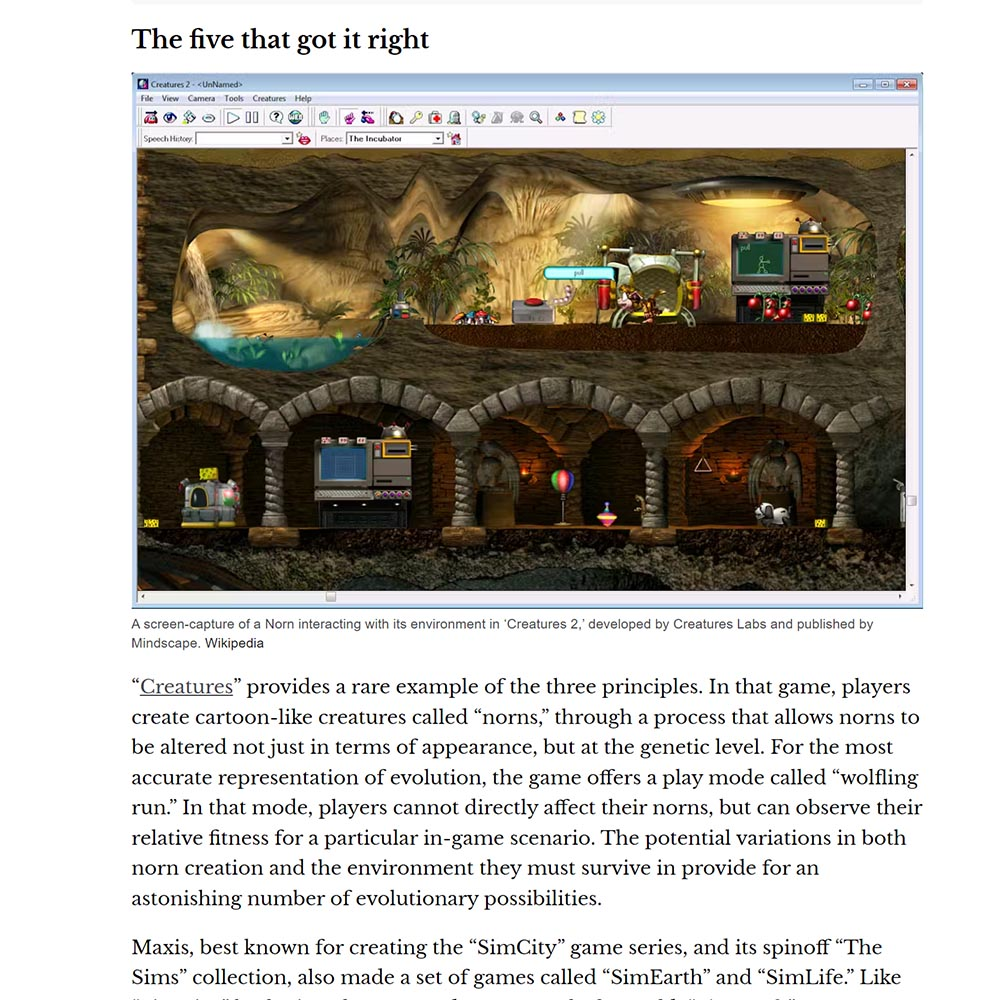
\includegraphics[width=1\linewidth,height=\textheight,keepaspectratio]{images/fig091.jpg}

\subsubsection*{Industry Examples}\label{industry-examples}
\addcontentsline{toc}{subsubsection}{Industry Examples}

There are many different ways to report research in industry. Some of the most common methods include:

\textbf{White papers}: White papers are a type of report that is commonly used in industry to present research findings to a specific audience. They are typically written in a clear and concise style and focus on a specific topic.


\includegraphics[width=1\linewidth,height=\textheight,keepaspectratio]{images/white_paper.png}

\textbf{Executive summaries}: Executive summaries are a brief overview of a white paper or other research report. They are typically written for senior executives and other decision-makers.

\textbf{Presentations}: Presentations are a way to share research findings with a live audience. They can be given at company meetings, conferences, or other events.

\textbf{Blogs and social media}: Blogs and social media can be used to share research findings with a wider audience. They are a good way to communicate research in a more informal way.

\textbf{Press releases}: Press releases are a way to share research findings with the media. They are typically written in a clear and concise style and focus on the key findings of the research.

\textbf{Technical reports}: Technical reports are a detailed document that describes the research methods and findings. They are typically written for a technical audience.

The best way to report research in industry depends on the specific research project and the intended audience. However, all of these methods can be effective ways to communicate research findings and to contribute to the industry community.

\section{Finding Research Papers}\label{finding-research-papers}

Finding research papers is an essential skill for students and researchers alike. Research papers are the backbone of academic work, providing the evidence, insights, and foundations necessary for developing new theories, testing hypotheses, and building knowledge. Whether you're writing a paper, preparing a presentation, or simply expanding your understanding of a topic, knowing how to locate and access research papers efficiently is crucial. Below are some effective strategies to help you find the research papers you need.

\subsection*{Check Your University Library}\label{check-your-university-library}
\addcontentsline{toc}{subsection}{Check Your University Library}

Your university library is one of the most valuable resources for finding research papers. University libraries provide access to a vast array of academic materials, including books, journals, and databases that are often not available for free online. Here's how to make the most of your university library's resources:

\href{https://www.siue.edu/lovejoy-library/ask-a-librarian/}{\textbf{Talk to a Librarian}}\textbf{.} Librarians are highly trained in information retrieval and can assist you in finding the most relevant and high-quality research papers for your topic. They can guide you to the right databases, help you refine your search strategies, and even suggest keywords or subject headings you might not have considered. Many libraries also offer personalized research consultations where you can get in-depth assistance on your specific research needs.

\href{https://i-share-sie.primo.exlibrisgroup.com/discovery/search?vid=01CARLI_SIE:CARLI_SIE&lang=en}{\textbf{Use the Library's Online Catalog}}\textbf{.} The online catalog is a powerful tool that allows you to search the entire collection of your university library, including books, journals, e-books, and other materials. You can narrow down your results by using specific search terms or filters to find the most relevant research papers. Most catalogs also allow you to see whether the materials are available physically in the library or online.

\href{https://libguides.siue.edu/az.php}{\textbf{Access the Library's Databases}}\textbf{.} University libraries subscribe to many academic databases that provide access to thousands of scholarly journals, articles, and other resources. These databases are often organized by subject, making finding research papers in your field of study easier. Popular databases include JSTOR, ProQuest, and EBSCOhost, among others. Databases can usually be searched by keyword, author, or subject, and many offer advanced search options that allow you to combine terms and apply filters to get the best results.

\subsection*{Use a specialized search engine.}\label{use-a-specialized-search-engine.}
\addcontentsline{toc}{subsection}{Use a specialized search engine.}

Specialized search engines are designed to search for specific types of information, such as research articles. Here are some tips on how to use a specialized search engine to find research articles:

\subsubsection*{Where to Search}\label{where-to-search}
\addcontentsline{toc}{subsubsection}{Where to Search}

When searching for research articles, knowing where to search is just as important as how you search. Specialized search engines are designed specifically for academic and scholarly materials, making them ideal tools for finding high-quality research papers. Unlike general search engines like Google, these specialized tools index scholarly content such as journal articles, conference papers, and theses. Below are some key specialized search engines and tips on how to choose the right one for your research needs.

Selecting the appropriate search engine depends on your research topic. If you're studying medicine or biology, PubMed should be your first choice. For engineering and technology, IEEE Xplore and ACM Digital Library are more suitable. If your research spans multiple disciplines, starting with Google Scholar, Web of Science, or Scopus may yield the broadest results.

\textbf{1. Google Scholar}

Google Scholar is one of the most widely used academic search engines. It provides access to a broad range of scholarly articles, theses, books, conference papers, and patents across various disciplines. It's a good starting point for most research topics due to its extensive coverage.

\href{https://scholar.google.com/}{
\includegraphics[width=1\linewidth,height=\textheight,keepaspectratio]{images/google-scholar.jpg}}

\textbf{2. PubMed}

PubMed is the go-to search engine for research in the biomedical and life sciences. It offers a comprehensive collection of articles from journals in medicine, biology, and health-related fields. If your research is in these areas, PubMed is an indispensable resource.

\href{https://pubmed.ncbi.nlm.nih.gov/}{
\includegraphics[width=1\linewidth,height=\textheight,keepaspectratio]{images/pubmed.jpg}}

\textbf{3. Web of Science}

Web of Science is a powerful tool that covers a wide array of disciplines, including the sciences, social sciences, arts, and humanities. It is particularly useful for citation tracking, allowing you to see how often an article has been cited by others, which can help you gauge its impact and relevance.

\href{https://go.openathens.net/redirector/siue.edu?url=https\%3A\%2F\%2Fwebofknowledge.com\%2FWOS}{
\includegraphics[width=1\linewidth,height=\textheight,keepaspectratio]{images/web-of-science.jpg}}

\textbf{4. Scopus}

Scopus is another multidisciplinary database, with an extensive collection of articles in the sciences, technology, medicine, social sciences, and more. Scopus also provides citation analysis, making it useful for understanding the influence of a particular study within its field.

\href{https://www.scopus.com/home.uri}{
\includegraphics[width=1\linewidth,height=\textheight,keepaspectratio]{images/scopus.jpg}}

\textbf{5. IEEE Xplore}

IEEE Xplore is the premier search engine for research in electrical engineering, computer science, and electronics. It indexes a vast number of conference papers, journal articles, and standards published by the IEEE.

\href{https://ieeexplore.ieee.org/Xplore/home.jsp}{
\includegraphics[width=1\linewidth,height=\textheight,keepaspectratio]{images/ieee-xplore.jpg}}

\textbf{6. ACM Digital Library}

The ACM Digital Library is essential for computer science research, offering a wide range of articles, conference proceedings, and other publications by the Association for Computing Machinery. It is particularly valuable for topics in software engineering, computer systems, and human-computer interaction.

\href{https://dl.acm.org/}{
\includegraphics[width=1\linewidth,height=\textheight,keepaspectratio]{images/acm-digital-library.jpg}}

\subsubsection*{How to Search}\label{how-to-search}
\addcontentsline{toc}{subsubsection}{How to Search}

Once you've chosen where to search, understanding how to effectively use these tools is crucial for finding the most relevant and high-quality research articles. Below are strategies to help you optimize your search process.

\textbf{1. Use Keywords Effectively}

Keywords are the foundation of any search. Start by identifying the main concepts of your research topic. For example, if you're researching the effects of social media on mental health, your main keywords might be ``social media,'' ``mental health,'' and ``impact.'' Input these keywords into your chosen search engine to begin your search.

\textbf{2. Utilize Advanced Search Features}

Most specialized search engines offer advanced search options that allow you to refine your search. You can often specify criteria such as:

\begin{itemize}
\tightlist
\item
  \textbf{Publication Date:} Limit your results to recent publications to ensure the information is up-to-date.
\item
  \textbf{Language:} If you're only interested in articles written in a specific language, you can filter results accordingly.
\item
  \textbf{Document Type:} Narrow down your search to only include journal articles, reviews, conference papers, etc.
\end{itemize}

For instance, in Google Scholar, you can access these options by clicking on ``Advanced Search,'' which allows you to combine keywords with Boolean operators, search within specific journals, or exclude certain terms from your results.

\textbf{3. Use Quotation Marks for Exact Phrases}

When searching for specific phrases, using quotation marks can help ensure that the search engine looks for the words together in the exact order you've specified. For example, searching for ``impact of social media on mental health'' will return results where this phrase appears as is, rather than finding articles where these words appear separately.

\textbf{4. Apply Boolean Operators}

Boolean operators (AND, OR, NOT) are powerful tools for refining your search:

\begin{itemize}
\tightlist
\item
  \textbf{AND:} Use AND to narrow your search. For example, ``social media AND mental health'' will return articles that contain both terms.
\item
  \textbf{OR:} Use OR to broaden your search by including synonyms or related terms. For example, ``social media OR social networks'' will return articles that include either term.
\item
  \textbf{NOT:} Use NOT to exclude unwanted terms. For example, ``social media NOT Facebook'' will exclude articles that specifically focus on Facebook.
\end{itemize}

\begin{figure}
\centering
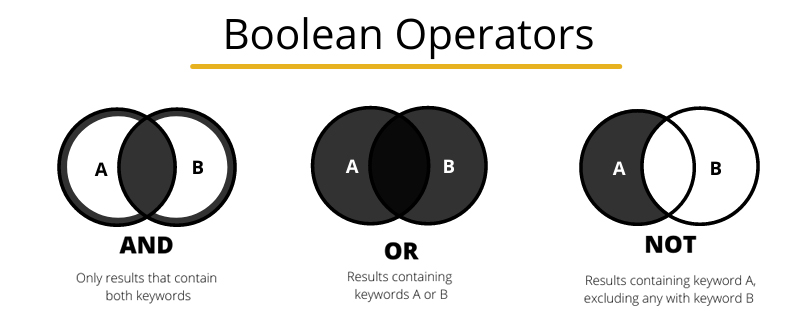
\includegraphics[width=1\linewidth,height=\textheight,keepaspectratio]{images/boolean.jpg}
\caption{Boolean Operators}
\end{figure}

\textbf{5. Read and Evaluate Search Results Carefully}

After conducting your search, take the time to review the results carefully. Pay attention to the title, abstract, and keywords of each article to determine its relevance to your research. Ensure that the articles are published in reputable journals, have undergone peer review, and are authored by credible experts in the field.

\textbf{6. Use Filters to Narrow Down Results}

Many specialized search engines provide filters that allow you to narrow down results by various criteria, such as year of publication, subject area, or type of document. For instance, if you are looking for the most recent studies on a topic, you can filter your search results to only include articles published in the last five years.

\textbf{7. Refer to Help Documentation}

If you're unfamiliar with a particular search engine, refer to its help documentation. These guides often include tips on using advanced search features, understanding search results, and optimizing your search queries. For example, Google Scholar's help page provides explanations on how to refine searches, save citations, and set up alerts for new research.

By combining the right search engine with effective search strategies, you can efficiently find the research articles you need for your academic work.

\subsection*{Using Social Media to Find Research Articles}\label{using-social-media-to-find-research-articles}
\addcontentsline{toc}{subsection}{Using Social Media to Find Research Articles}

Social media has become a powerful tool for academics and researchers, providing a platform to share, discover, and discuss research articles. By leveraging the features of various social media platforms, you can stay informed about the latest developments in your field, find relevant research articles, and connect with other scholars. Below are some effective strategies for using social media to find research articles.

\subsubsection*{1. Follow Researchers and Research Institutions}\label{follow-researchers-and-research-institutions}
\addcontentsline{toc}{subsubsection}{1. Follow Researchers and Research Institutions}

One of the most direct ways to stay updated with the latest research is by following individual researchers, academic institutions, and research organizations on social media. Many scholars use platforms like Twitter, LinkedIn, and ResearchGate to share their latest publications, conference presentations, and ongoing projects. By following these accounts, you can receive updates on new research articles as soon as they are published. Additionally, institutions often share open access articles, preprints, and links to publications that might be behind paywalls elsewhere, providing valuable resources for your own research.

\begin{itemize}
\tightlist
\item
  \textbf{Tip:} When following researchers, consider looking at their followers and who they follow as well. This can help you find other relevant scholars and institutions in your area of interest.
\end{itemize}

\subsubsection*{2. Use Relevant Hashtags}\label{use-relevant-hashtags}
\addcontentsline{toc}{subsubsection}{2. Use Relevant Hashtags}

Hashtags on social media platforms like Twitter and Instagram serve as powerful tools for categorizing content and making it discoverable to a broader audience. Researchers and institutions often use specific hashtags related to their field, research topic, or academic events. By searching for or following these hashtags, you can easily find posts related to recent research articles, discussions on emerging trends, and links to relevant studies.

\begin{itemize}
\tightlist
\item
  \textbf{Example:} Searching for hashtags such as \#OpenAccess, \#ScienceTwitter, \#AcademicChatter, or discipline-specific tags like \#PsychResearch or \#ClimateScience can lead you to valuable research articles and academic discussions.
\end{itemize}

\subsubsection*{3. Join Research Groups and Communities}\label{join-research-groups-and-communities}
\addcontentsline{toc}{subsubsection}{3. Join Research Groups and Communities}

Social media platforms host numerous groups and communities dedicated to specific research fields or interdisciplinary topics. These groups, which can be found on platforms like Facebook, LinkedIn, and Reddit, are spaces where researchers share their work, seek advice, and discuss recent findings. Joining these groups allows you to engage with peers, discover articles that might not be widely publicized, and gain insights from ongoing academic discussions.

\begin{itemize}
\tightlist
\item
  \textbf{Tip:} When joining a group, take the time to introduce yourself and share your research interests. Active participation can lead to more meaningful connections and opportunities to find relevant research articles.
\end{itemize}

\subsubsection*{4. Attend Online Conferences and Workshops}\label{attend-online-conferences-and-workshops}
\addcontentsline{toc}{subsubsection}{4. Attend Online Conferences and Workshops}

The shift to virtual events has made it easier than ever to attend academic conferences and workshops from anywhere in the world. These events are often live-streamed on social media platforms or have dedicated hashtags for participants to follow along and discuss. Attending these online events allows you to access presentations, papers, and discussions that are directly relevant to your research. Additionally, many conferences post recordings of sessions or provide access to conference papers after the event, giving you further opportunities to explore new research.

\begin{itemize}
\tightlist
\item
  \textbf{Tip:} After attending a session, engage with the speakers and attendees on social media by sharing your thoughts or asking questions. This can help you build a network of contacts who may share additional resources or research articles.
\end{itemize}

\subsubsection*{Specific Social Media Platforms to Use}\label{specific-social-media-platforms-to-use}
\addcontentsline{toc}{subsubsection}{Specific Social Media Platforms to Use}

\textbf{Twitter:} Twitter is an excellent platform for real-time research updates, especially by following researchers and journals and using hashtags. Many academic communities thrive on Twitter, making it a rich resource for finding the latest studies.

\textbf{LinkedIn:} LinkedIn is ideal for connecting with professionals and academics in your field. Researchers often share their publications and discuss their implications on LinkedIn, making it a valuable platform for professional networking and discovering research articles.

\textbf{ResearchGate:} ResearchGate is a dedicated social networking site for researchers. It allows you to follow researchers, access their publications, request full-text articles, and engage in discussions. It's particularly useful for finding peer-reviewed research and collaborating with other scholars.

\textbf{Evaluating Sources on Social Media}

While social media is a powerful tool for discovering research articles, it is crucial to critically evaluate the sources you find. Not all articles shared on social media are of high quality or come from reputable journals. Always consider the credibility of the author, the publication venue, and the methodology of the research before incorporating it into your own work. If in doubt, consult a librarian or an academic advisor for further guidance.

\subsection*{Contacting Experts in Your Field}\label{contacting-experts-in-your-field}
\addcontentsline{toc}{subsection}{Contacting Experts in Your Field}

In addition to using social media, directly contacting experts in your field can be an invaluable way to find research articles and gain deeper insights into your study area. Experts can provide recommendations for key papers, suggest emerging research areas, and even share unpublished work that may not yet be available in databases.

\subsubsection*{1. Talk to Your Professors or Advisors}\label{talk-to-your-professors-or-advisors}
\addcontentsline{toc}{subsubsection}{1. Talk to Your Professors or Advisors}

Your professors and academic advisors are often the best starting point when seeking expert guidance. They have deep knowledge of the field, are familiar with the latest research, and can point you toward seminal papers or recommend specific articles that are highly relevant to your research. Moreover, they may have access to articles or resources that are not available to students, which can further enrich your research.

\begin{itemize}
\tightlist
\item
  \textbf{Tip:} When approaching your professors, be specific about your research topic and what you hope to learn. This will help them provide more targeted recommendations.
\end{itemize}

\subsubsection*{2. Attend Conferences and Workshops}\label{attend-conferences-and-workshops}
\addcontentsline{toc}{subsubsection}{2. Attend Conferences and Workshops}

Conferences and workshops are excellent venues for meeting experts and learning about the latest research. These events often feature presentations from leading scholars, providing an opportunity to hear about their work directly. After a presentation, don't hesitate to approach the speaker with questions or requests for further reading. Many experts are happy to share their articles or direct you to where you can find them.

\begin{itemize}
\tightlist
\item
  \textbf{Tip:} Prepare a list of questions or topics of interest before attending a conference. This will help you maximize the networking opportunities and identify experts who can assist with your research.
\end{itemize}

\subsubsection*{3. Read Research Blogs and Newsletters}\label{read-research-blogs-and-newsletters}
\addcontentsline{toc}{subsubsection}{3. Read Research Blogs and Newsletters}

Many experts maintain blogs or contribute to newsletters that discuss their research and developments in the field. These platforms are often more accessible than academic journals and provide insights into the latest research trends. Following these blogs or subscribing to newsletters can keep you informed about new publications and give you a more nuanced understanding of ongoing debates in your field.

\begin{itemize}
\tightlist
\item
  \textbf{Tip:} Look for blogs that are peer-reviewed or written by recognized experts in the field to ensure the information is reliable.
\end{itemize}

\subsubsection*{4. Use Social Media to Connect with Experts}\label{use-social-media-to-connect-with-experts}
\addcontentsline{toc}{subsubsection}{4. Use Social Media to Connect with Experts}

As mentioned earlier, social media platforms are also useful for connecting with experts. By following researchers, engaging with their posts, and joining relevant groups, you can build relationships that may lead to further collaboration or recommendations for research articles. Many researchers are open to sharing their work or discussing their findings with interested peers, especially if you approach them respectfully and with clear questions.

\begin{itemize}
\tightlist
\item
  \textbf{Tip:} When reaching out to an expert on social media, always introduce yourself and explain why you are interested in their work. Be concise and professional in your communication to make a positive impression.
\end{itemize}

\subsubsection*{Finding and Contacting Experts}\label{finding-and-contacting-experts}
\addcontentsline{toc}{subsubsection}{Finding and Contacting Experts}

\textbf{Search by Name or Topic:} Use academic databases, professional organizations, or specialized directories to find experts in your field. You can search by specific research topics or by the names of researchers who have published influential work in your area of interest.

\textbf{Look for Published Authors:} Identify experts by looking at the authors of the research articles you find through databases like Google Scholar or Scopus. Those who frequently publish in reputable journals are likely to be well-established in their field.

\textbf{Seek Out Conference Presenters:} Experts who present at conferences are often leaders in their field. You can find information about upcoming conferences on the websites of professional organizations. After identifying relevant presenters, consider reaching out to them with specific questions or requests for further reading.

\textbf{Engage with Active Social Media Users:} Many researchers are active on platforms like Twitter, LinkedIn, and ResearchGate. By engaging with their content---whether through likes, comments, or direct messages---you can start a conversation that may lead to valuable research recommendations.

When contacting experts, be mindful of their time and make your requests clear and concise. Express gratitude for their assistance and follow up with any additional questions you may have after your initial conversation. Building a professional relationship with experts in your field can significantly enhance your research and provide you with insights that are not readily available through other means.

\section{Readings Research Papers}\label{readings-research-papers}

There are many different approaches to reading a research paper, but these are some of the most effective ones.

\subsection*{The three-pass approach.}\label{the-three-pass-approach.}
\addcontentsline{toc}{subsection}{The three-pass approach.}

The three-pass approach to reading a research paper is a method of reading a paper in three stages, each with a specific goal.

\textbf{The first pass}. This is a quick scan to capture a high-level view of the paper. You should read the title, abstract, and introduction carefully, and then skim the rest of the paper, paying attention to the headings and subheadings. The goal of this pass is to get a general understanding of what the paper is about, its main points, and its contributions to the field.

\textbf{The second pass}: This is a more detailed reading of the paper. You should read the introduction and conclusion carefully, and then read the rest of the paper in more detail, paying attention to the methods, results, and discussion. The goal of this pass is to understand the paper's arguments and evidence, and to assess its strengths and weaknesses.

\textbf{The third pass}: This is a critical reading of the paper. You should read the paper carefully, taking notes and challenging the author's assumptions and conclusions. The goal of this pass is to fully understand the paper and to be able to critically evaluate its claims.

\subsection*{The question-based approach.}\label{the-question-based-approach.}
\addcontentsline{toc}{subsection}{The question-based approach.}

The question-based approach to reading a research paper is a method of reading a paper by asking questions about the paper as you read. This approach can help you to focus your reading and to ensure that you understand the key points of the paper.

Here are some questions that you can ask yourself as you read a research paper:

\begin{itemize}
\item
  What is the purpose of the paper?
\item
  What are the main questions that the paper addresses?
\item
  What are the key findings of the paper?
\item
  How does the paper contribute to the existing body of knowledge?
\item
  What are the strengths and weaknesses of the paper?
\item
  How does the paper relate to my own research interests?
\end{itemize}

You can also ask more specific questions that are relevant to the specific paper that you are reading. For example, if you are reading a paper about a new medical treatment, you might ask questions about the safety and effectiveness of the treatment.

The question-based approach can be used in conjunction with the three-pass approach to reading a research paper. In the first pass, you can ask general questions about the paper to get a sense of what it is about. In the second pass, you can ask more specific questions to understand the paper in more detail. In the third pass, you can critically evaluate the paper by asking questions about its methods, findings, and conclusions.

The question-based approach is a flexible method that can be adapted to your own needs and preferences. By asking questions as you read, you can improve your understanding of research papers and your ability to critically evaluate their claims. The question-based approach is a valuable tool for reading and understanding research papers. By asking questions as you read, you can improve your comprehension and critical thinking skills.

\subsection*{The active reading approach.}\label{the-active-reading-approach.}
\addcontentsline{toc}{subsection}{The active reading approach.}

Active reading is a method of reading that involves engaging with the text in a thoughtful and critical way. It is different from passive reading, which is simply reading the text without thinking about it.

Active reading can be used to read any type of text, but it is especially important for reading research papers. Research papers are often dense and technical, so it is important to be actively engaged in order to understand them.

Here are some tips for active reading:

\textbf{Ask questions}: As you read, ask yourself questions about the text. What is the author's purpose? What are the main points? What evidence does the author provide to support their claims?

\textbf{Take notes}: Taking notes can help you to remember the key points of the text and to track your progress. You can take notes in the margins of the text, or you can use a separate notebook.

\textbf{Summarize}: After each section of the text, summarize the key points in your own words. This will help you to solidify your understanding of the text.

\textbf{Discuss the text with others}: Talking to others about a text can help you to gain new insights and perspectives.

\textbf{Annotate the text}: Annotating the text means making notes and comments in the margins. This can help you to highlight important passages, ask questions, and make connections between different parts of the text.

\textbf{Use a highlighter}: Highlighting important passages can help you to focus your attention and to remember the key points of the text.

\textbf{Take a break}: Don't try to read a research paper in one sitting. Take breaks to refresh your mind and to come back to the text with fresh eyes.

Active reading takes time and effort, but it is a valuable skill for anyone who wants to learn and grow. By actively reading research papers, you can improve your comprehension, critical thinking skills, and ability to learn new things.

\subsection*{The collaborative reading approach.}\label{the-collaborative-reading-approach.}
\addcontentsline{toc}{subsection}{The collaborative reading approach.}

This approach involves reading the paper with a partner or group of people. This can be helpful for getting different perspectives on the paper and for identifying areas where you need clarification.

No matter which approach you choose, it is important to take your time and read the paper carefully. Research papers can be dense and challenging, but they can also be very rewarding. By taking the time to read them carefully, you can learn a lot about your field and contribute to the advancement of knowledge. The question-based approach is a valuable tool for reading and understanding research papers. By asking questions as you read, you can improve your comprehension and critical thinking skills.

\chapter{Defining Scope}\label{defining-scope}

\section{Conceptual Definitions and Operationalization}\label{conceptual-definitions-and-operationalization}

In mass media research, defining and measuring abstract concepts is essential for creating a clear and structured approach to studying communication phenomena. Two critical processes forming this approach's foundation are \textbf{conceptual definition} and \textbf{operationalization}. Understanding these processes allows researchers to build a solid framework for their inquiries, ensuring they accurately capture and analyze the complex elements of media-related phenomena.

\subsection*{Conceptual Definitions}\label{conceptual-definitions}
\addcontentsline{toc}{subsection}{Conceptual Definitions}

A \textbf{concept} is a broad, abstract idea that encapsulates a specific phenomenon researchers want to explore. Concepts act as the foundational building blocks of research, helping scholars focus on particular aspects of media and communication. In mass media research, common concepts include ``media influence,'' ``public opinion,'' and ``audience engagement.'' Each of these concepts represents a broad idea that requires further refinement before it can be effectively studied.

\begin{figure}
\centering
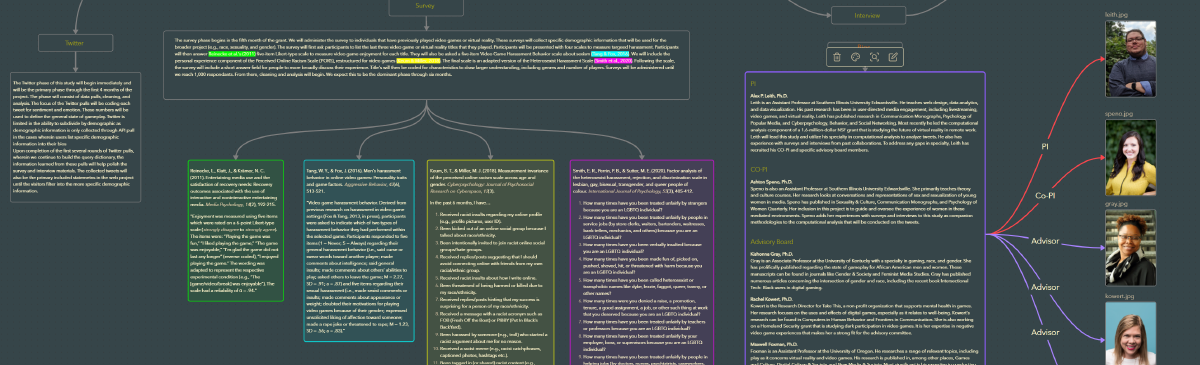
\includegraphics[width=1\linewidth,height=\textheight,keepaspectratio]{images/concept-map.png}
\caption{Example of a concept map during the early stage of project design.}
\end{figure}

For example, take the concept of ``media influence.'' It represents a wide range of possible effects that media could have on individuals or society. These effects might include shaping public opinion, influencing behavior, or reinforcing cultural values. The broad nature of such a concept necessitates clear definition. Researchers need to specify which aspect of media influence they are focusing on to conduct meaningful analysis.

In another example, consider ``audience engagement.'' This concept could refer to various behaviors, such as how audiences consume, interact with, and share media content. Before conducting research on audience engagement, a scholar must define what they mean by the term. Does it refer to passive consumption, like viewing time, or active participation, such as comments and shares on social media? These distinctions are critical because they affect how the concept will be examined and understood.

By narrowing down these broad concepts into specific, clearly defined terms, researchers can target their investigations more effectively. A well-defined concept is crucial for both focusing the scope of a study and ensuring that findings are relevant and actionable.

\subsection*{Operationalization}\label{operationalization}
\addcontentsline{toc}{subsection}{Operationalization}

Once a concept has been clearly defined, the next step is \textbf{operationalization}, which involves transforming abstract concepts into measurable variables. Operationalization bridges the gap between theoretical ideas and empirical research, allowing researchers to gather observable, quantifiable data.

For example, after defining ``audience engagement,'' a researcher must determine how to measure it. Operationalization involves selecting appropriate indicators that accurately reflect the concept. In the case of audience engagement, possible indicators might include metrics like the number of likes, comments, and shares a piece of media content receives. These indicators provide tangible data that can be used to measure audience interaction.

Similarly, if a study focuses on ``media influence,'' operationalization might involve measuring changes in public opinion before and after exposure to a particular media campaign. This could be done through surveys or experiments designed to capture shifts in attitudes or beliefs, allowing researchers to quantify the concept of media influence meaningfully.

Choosing appropriate indicators is crucial to operationalization, as the selected measures must accurately reflect the concept being studied. Poor operationalization can lead to unreliable or invalid results, undermining the overall integrity of the research.

\subsection*{The Importance of Conceptual Definitions and Operationalization}\label{the-importance-of-conceptual-definitions-and-operationalization}
\addcontentsline{toc}{subsection}{The Importance of Conceptual Definitions and Operationalization}

Defining and operationalizing concepts are vital because they form the backbone of any empirical study. Without clear definitions, researchers risk ambiguity, making it difficult to draw valid conclusions from their findings. Similarly, without precise operationalization, measuring abstract ideas in a way that produces reliable and valid data becomes impossible.

Given the complex and often intangible nature of the phenomena studied, these processes are particularly important in mass media research. Concepts like media influence, audience engagement, and public opinion are multifaceted and require careful conceptualization and measurement. By clearly defining their concepts and developing sound operational definitions, researchers ensure their studies are rigorous and meaningful, contributing to a deeper understanding of media processes and effects.

This knowledge is essential for conducting reliable research in mass media, as it ensures that the abstract ideas central to media studies can be systematically examined and understood. Through conceptual definition and operationalization, researchers can turn theoretical ideas into concrete, measurable realities, paving the way for studies that yield insightful and actionable findings.

\section{Identifying Independent and Dependent Variables}\label{identifying-independent-and-dependent-variables}

Understanding independent and dependent variables is fundamental in structuring research, particularly when studying cause-and-effect relationships. These variables are the backbone of empirical research, allowing researchers to manipulate one factor to observe its influence on another. In mass media research, identifying and distinguishing between independent and dependent variables is crucial for defining clear research questions, testing hypotheses, and producing meaningful findings.

\subsection*{Independent Variables}\label{independent-variables}
\addcontentsline{toc}{subsection}{Independent Variables}

The \textbf{independent variable (IV)} is the factor that the researcher manipulates or categorizes to examine its effect on another variable. It represents the ``cause'' in a cause-and-effect relationship. In mass media research, the independent variable is often a media-related factor or characteristic that the researcher changes to observe its impact. For example, in a study exploring the effect of media content on audience engagement, the type of media content---such as news, entertainment, or educational programs---would be the independent variable. The researcher manipulates the content type to examine how it influences the outcome, which is the dependent variable.

To clarify, imagine a study investigating how different advertising formats influence consumer behavior. In this case, the independent variable could be the advertisement format---whether it is a video, banner ad, or social media post. By altering the format, the researcher can observe how these changes affect consumer behavior, such as click-through rates or purchasing decisions. The independent variable is the element you control or modify to determine its impact on the dependent variable.

\begin{figure}
\centering
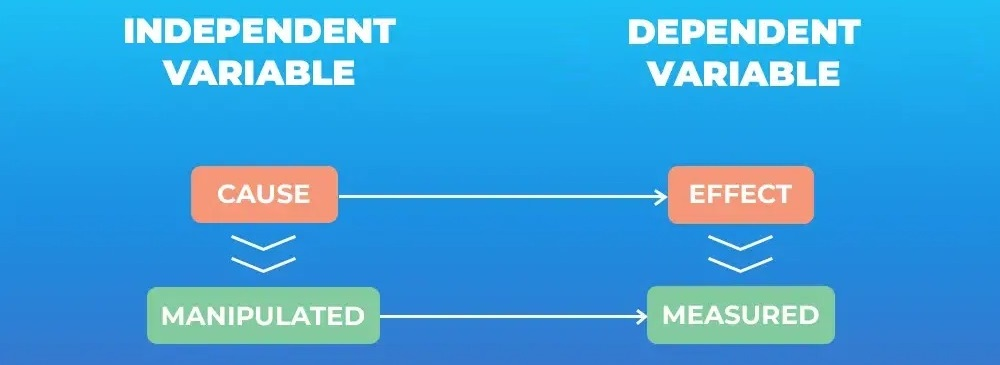
\includegraphics[width=1\linewidth,height=\textheight,keepaspectratio]{images/ind-dep.jpg}
\caption{Difference between Independent and Dependent Variables}
\end{figure}

\subsection*{Dependent Variables}\label{dependent-variables}
\addcontentsline{toc}{subsection}{Dependent Variables}

The \textbf{dependent variable (DV)} is the outcome measured in response to changes in the independent variable. It represents the ``effect'' in the cause-and-effect relationship. The dependent variable is what the researcher observes and records, indicating how the independent variable influences the phenomenon under study.

In mass media research, the dependent variable could be audience behavior, perceptions, or attitudes. For example, in a study measuring the impact of media content on engagement, the dependent variable might be audience engagement. This could be quantified by metrics such as the number of comments, likes, shares, or the time spent viewing the content. The researcher examines these metrics to see if and how they are influenced by changes in the independent variable, such as the type or style of media content presented.

Consider another example: a study exploring the effect of headline styles on readers' perceptions of news credibility. The dependent variable could be the credibility score that participants assign to each article after reading it. By measuring this score, the researcher can assess whether variations in the headline (the independent variable) have a measurable impact on how credible readers perceive the news to be.

\subsection*{Cause-and-Effect}\label{cause-and-effect}
\addcontentsline{toc}{subsection}{Cause-and-Effect}

The relationship between independent and dependent variables is essential for understanding how different aspects of media influence behavior, attitudes, or perceptions. For example, if you are studying the effect of social media usage on academic performance, social media usage would be the independent variable. In contrast, academic performance, measured through test scores or grades, would be the dependent variable. In this case, the researcher is investigating whether the amount of time spent on social media influences academic outcomes.

Understanding this relationship allows researchers to test specific hypotheses about media effects. For instance, if you hypothesize that ``increased exposure to political ads leads to higher voter turnout,'' the independent variable is the exposure to political ads, and the dependent variable is voter turnout. By manipulating the independent variable---changing the level of exposure to political ads---you can measure its effect on the dependent variable, voter turnout.

\subsection*{The Role of Variables in Experimental Design}\label{the-role-of-variables-in-experimental-design}
\addcontentsline{toc}{subsection}{The Role of Variables in Experimental Design}

Correctly identifying independent and dependent variables is crucial for designing experiments and interpreting results in mass media research. Independent variables allow researchers to explore different media formats, messages, or platforms, while dependent variables help measure the outcomes of those explorations. This structured approach provides insights into the effects of media on individuals and society.

For instance, a researcher investigating how different frequencies of advertisement exposure affect brand recall must clearly define the independent variable (frequency of advertisement exposure) and the dependent variable (brand recall). Understanding these variables enables the researcher to design an experiment that tests specific hypotheses, yielding actionable insights about advertising strategies and their effectiveness.

By mastering the identification of independent and dependent variables, you can design robust studies that accurately test your hypotheses, contribute to mass media research, and offer meaningful conclusions. This knowledge is critical for conducting your research and evaluating the work of others, allowing you to critically assess the validity and reliability of existing studies in the academic literature.

\section{Formulating Research Questions}\label{formulating-research-questions}

A well-formulated research question is the foundation of any successful research study. In mass media research, the research question defines the focus and scope of your study, guiding both the theoretical framework and methodological approach. It sets the stage for hypothesis development, data collection, and analysis, ensuring the study remains focused and relevant.

Research questions serve as the guiding force behind your inquiry. They narrow broad topics into specific areas that can be explored systematically, allowing you to investigate particular aspects of media, communication, or social phenomena. Crafting a strong research question is an essential skill for any researcher, as it determines the direction and clarity of the entire study.

\subsection*{What Makes a Good Research Question?}\label{what-makes-a-good-research-question}
\addcontentsline{toc}{subsection}{What Makes a Good Research Question?}

A \textbf{good research question} should be clear, focused, and researchable. It should be specific enough to guide your study but broad enough for comprehensive exploration. In mass media research, the question should focus on a particular media-related phenomenon, effect, or relationship that can be empirically investigated.

For example, consider a broad topic like ``media influence.'' This is too vague to form a research question. However, by refining this idea, we can develop a more focused question: ``How does exposure to political news on social media affect young adults' trust in traditional news outlets?'' This question is specific, measurable, and directly related to a phenomenon that can be empirically tested.

A strong research question should also align with your research objectives. It should be framed in a way that reflects what you aim to discover or explain through your study. This helps ensure that your research remains coherent and that your findings are relevant to the broader field of mass media studies.

\subsection*{Types of Research Questions}\label{types-of-research-questions}
\addcontentsline{toc}{subsection}{Types of Research Questions}

Several types of research questions can be used in mass media research, depending on the goals of your study:

\begin{enumerate}
\def\labelenumi{\arabic{enumi}.}
\item
  \textbf{Descriptive Questions}: These questions describe a particular phenomenon's characteristics or features. For instance, ``What types of content do people engage with most on social media platforms?'' is a descriptive question because it aims to outline patterns or trends without exploring underlying causes.
\item
  \textbf{Comparative Questions}: These questions compare two or more groups, media forms, or phenomena. An example might be, ``How do perceptions of news credibility differ between users of traditional news media and social media?''
\item
  \textbf{Causal Questions}: These questions investigate the cause-and-effect relationships between variables. For example, ``Does exposure to violent video games increase aggressive behavior among adolescents?'' explores a potential causal relationship between media exposure and behavioral outcomes.
\item
  \textbf{Correlational Questions}: These questions examine the relationships between variables without implying causation. An example would be, ``Is there a correlation between social media usage and levels of political participation among young adults?''
\item
  \textbf{Exploratory Questions}: These questions are used when a topic is relatively new or underexplored. For instance, ``How do virtual influencers impact audience perceptions of authenticity in digital marketing?'' explores a contemporary issue with less established research.
\end{enumerate}

\subsection*{The Process of Developing a Research Question}\label{the-process-of-developing-a-research-question}
\addcontentsline{toc}{subsection}{The Process of Developing a Research Question}

Developing a research question begins with identifying a broad area of interest within the field of mass media. From there, you narrow down your focus to a specific topic that is both relevant and researchable. The key is to strike a balance between being too broad, which can make your study unwieldy, and too narrow, which may limit the scope and significance of your findings.

Here's a step-by-step approach to developing a research question:

\begin{enumerate}
\def\labelenumi{\arabic{enumi}.}
\item
  \textbf{Identify a General Topic}: Start with a broad area of interest within mass media, such as ``social media influence'' or ``news consumption patterns.''
\item
  \textbf{Conduct a Literature Review}: Review existing studies to understand what research has already been done on your topic. This will help you identify gaps in the literature that your study can address.
\item
  \textbf{Refine the Topic}: Based on your literature review, narrow your focus to a specific aspect of the topic. For example, instead of studying ``social media influence'' broadly, you might focus on ``the effects of social media on political engagement among young adults.''
\item
  \textbf{Formulate the Question}: Turn your refined topic into a clear, specific research question. For instance, ``How does social media usage influence political engagement among young adults during election campaigns?''
\item
  \textbf{Evaluate the Question}: Ensure your question is clear, focused, and feasible. Ask yourself if it can be answered through empirical research and if it aligns with your study's objectives.
\end{enumerate}

\subsection*{The Importance of Well-Defined Research Questions}\label{the-importance-of-well-defined-research-questions}
\addcontentsline{toc}{subsection}{The Importance of Well-Defined Research Questions}

A well-defined research question is crucial because it sets the parameters for your entire study. It informs the selection of your research methods, the design of your study, and the interpretation of your results. Without a clear question, research risks becoming unfocused, leading to ambiguous findings that may not contribute meaningfully to the field.

In mass media research, where the phenomena studied are often complex and multifaceted, a precise research question ensures that your study targets specific elements that can be measured and analyzed. For instance, a broad question like ``How does media influence society?'' is difficult to address due to its vagueness. In contrast, a specific question like ``How does exposure to negative political advertisements affect voter turnout among first-time voters?'' is focused and measurable, allowing for a more structured and insightful investigation.

By developing strong research questions, you enhance the clarity and focus of your study and contribute to the overall rigor of your research. A well-constructed research question leads to clear, actionable insights, ultimately advancing mass media research and deepening our understanding of the relationships between media, society, and communication.

Through carefully formulating research questions, you will be equipped to design studies that address key issues in media research, paving the way for hypotheses that can be systematically tested and analyzed.

\section{Constructing Hypotheses}\label{constructing-hypotheses}

In mass media research, constructing hypotheses is a critical step that allows researchers to test specific ideas and examine relationships between variables. Hypotheses structure your study, ensuring that the research is systematic and focused. When formulated correctly, hypotheses guide the collection and analysis of data, leading to sound, evidence-based conclusions.

Three key components are involved in hypothesis construction: the \textbf{null hypothesis (H0)}, the \textbf{alternative hypothesis (H1)}, and the \textbf{research question}. Each serves a unique function in the research process, helping to frame the study and focus the inquiry.

\subsection*{Null Hypothesis (H0)}\label{null-hypothesis-h0}
\addcontentsline{toc}{subsection}{Null Hypothesis (H0)}

The \textbf{null hypothesis (H0)} posits that there is no effect or no relationship between the variables under investigation. It serves as a starting point for your research, functioning as a baseline that your study aims to test. The null hypothesis is essential because it provides a clear, falsifiable statement that can be supported or rejected based on empirical evidence.

For example, consider a study examining the impact of media consumption on political attitudes. The null hypothesis might be: ``There is no difference in political attitudes between individuals who consume a high amount of media and those who consume a low amount.'' This hypothesis assumes that media consumption has no measurable effect on political attitudes. Your research aims to determine whether the data supports or refutes this assumption.

By beginning with the null hypothesis, researchers can remain objective in their approach. It creates a framework in which the data, rather than assumptions or biases, determines the outcome. If sufficient evidence is found to reject the null hypothesis, it suggests that a relationship or effect exists between the variables.

\begin{figure}
\centering
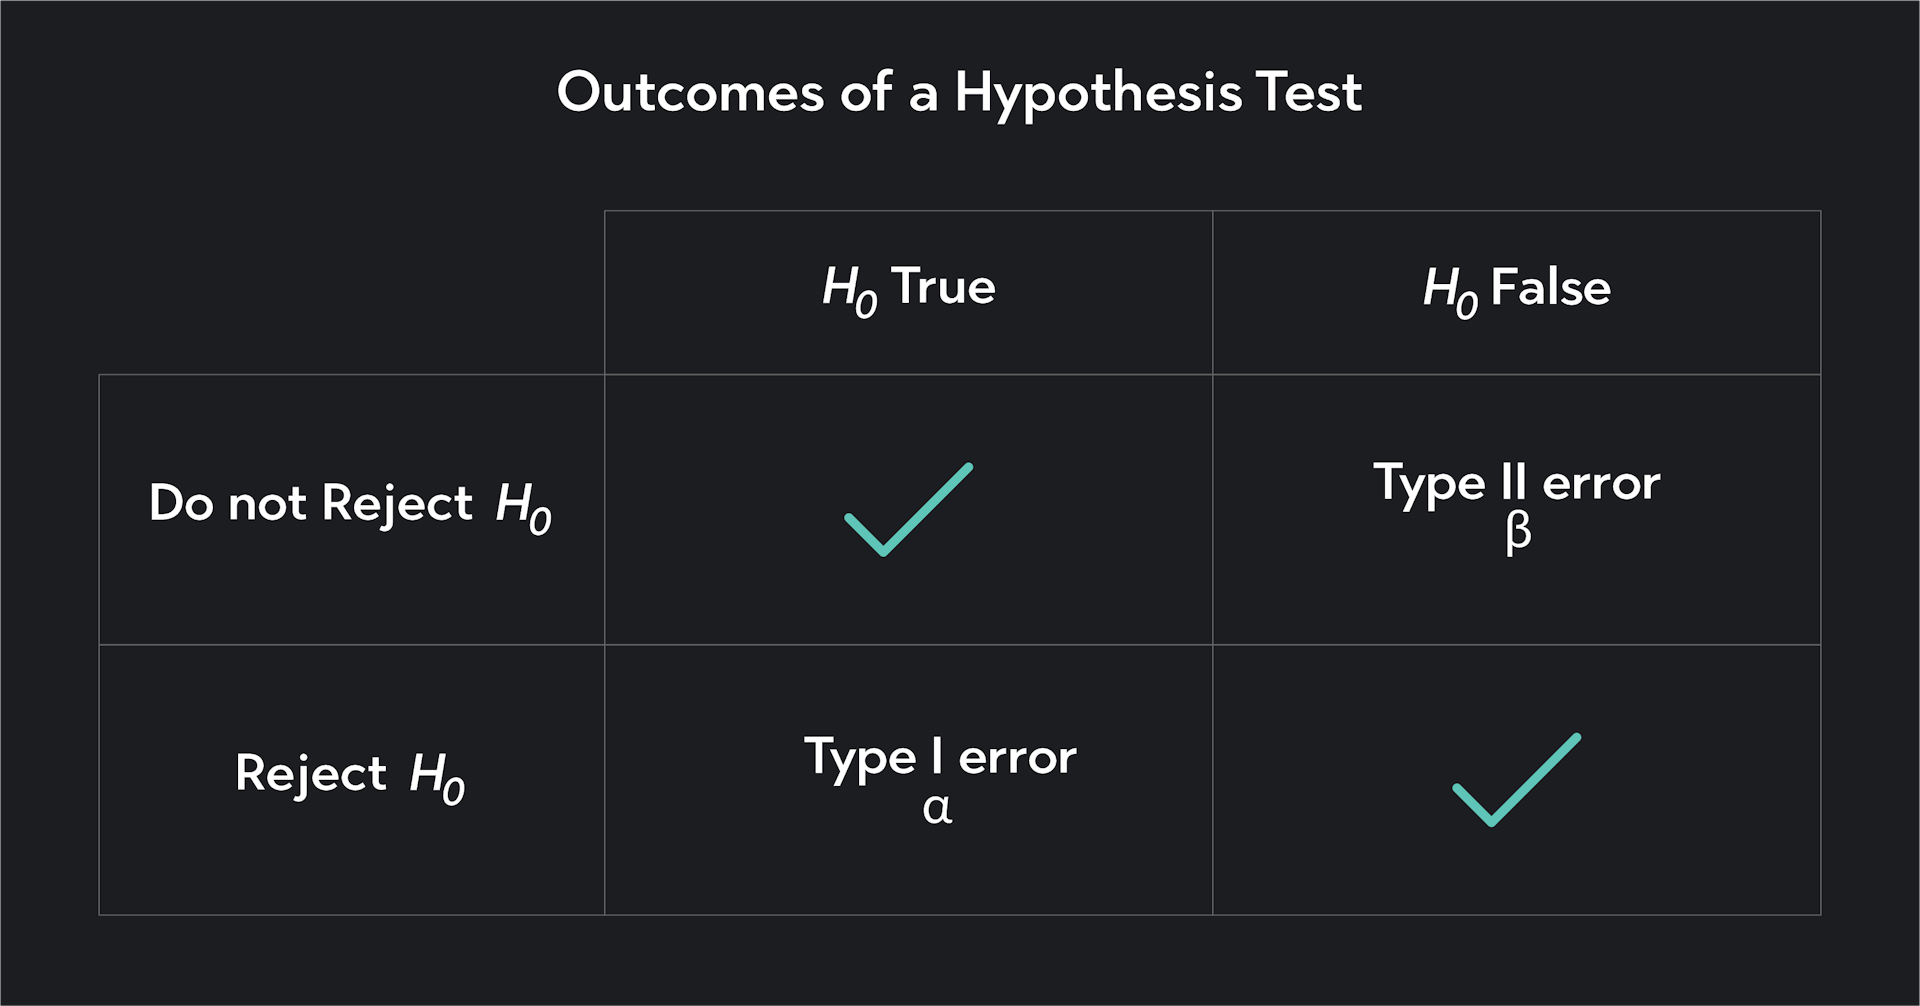
\includegraphics[width=1\linewidth,height=\textheight,keepaspectratio]{images/h0-ha.png}
\caption{Type Errors and Hypotheses}
\end{figure}

\subsection*{Alternative Hypothesis (H1)}\label{alternative-hypothesis-h1}
\addcontentsline{toc}{subsection}{Alternative Hypothesis (H1)}

In contrast to the null hypothesis, the \textbf{alternative hypothesis (H1)} asserts that there is a relationship or effect between the variables being studied. The alternative hypothesis directly opposes the null hypothesis, proposing that some change, difference, or relationship is present.

Continuing with the previous example, the alternative hypothesis might state: ``Individuals who consume a high amount of media have different political attitudes than those who consume a low amount.'' This hypothesis suggests that media consumption influences political attitudes. Your research will then gather evidence to support or refute this claim.

The alternative hypothesis is the hypothesis you are actively testing. It reflects your expectations about the relationship between variables and is usually derived from existing theory or literature. However, the evidence must show that the observed effects or relationships are statistically significant to accept the alternative hypothesis.

\subsection*{The Role of Hypotheses in Research Design}\label{the-role-of-hypotheses-in-research-design}
\addcontentsline{toc}{subsection}{The Role of Hypotheses in Research Design}

Constructing hypotheses is a central part of research design because it determines what to test and how to measure the relationships between variables. Hypotheses provide structure, helping researchers clarify their focus and ensure that their studies are methodologically sound.

In mass media research, hypotheses often explore how different forms of media affect behavior, attitudes, or social outcomes. For instance, a study may hypothesize that exposure to violent video games increases aggressive behavior in teenagers, or that social media usage is positively correlated with levels of political engagement. These hypotheses help frame the research question to allow for measurable outcomes, ensuring that the study can produce actionable insights.

By the end of this section, you should understand how to construct clear, testable hypotheses and formulate research questions that effectively guide your study. Mastering this process will allow you to design rigorous research that contributes valuable knowledge to the field of mass media, helping to explore and clarify the complex relationships between media and society.

\section{Levels of Measurement in Mass Media Research}\label{levels-of-measurement-in-mass-media-research}

Understanding the different levels of measurement is critical to designing sound research and conducting accurate data analysis in mass media studies. The level of measurement determines how data can be categorized, compared, and analyzed, influencing the types of statistical techniques you can apply. There are four primary levels of measurement: \textbf{nominal}, \textbf{ordinal}, \textbf{interval}, and \textbf{ratio}. Each offers a unique approach to organizing and quantifying data, and recognizing these distinctions is essential for conducting effective and meaningful research.

\subsection*{Nominal Level of Measurement}\label{nominal-level-of-measurement}
\addcontentsline{toc}{subsection}{Nominal Level of Measurement}

The \textbf{nominal level} involves classifying data into distinct categories that are mutually exclusive and lack any inherent order. Nominal data groups items based on shared characteristics, without implying any ranking or quantitative value. In mass media research, an example of nominal data could be classifying media content into genres, such as drama, comedy, or documentary. Each genre represents a category, but these categories cannot be ordered or ranked; they are simply different types.

Nominal data is useful for distinguishing between different media types or behaviors, allowing researchers to count occurrences and frequencies within each category. For example, you might count how many television shows fall into each genre. However, because nominal data does not involve any numerical value or rank, mathematical operations such as addition or subtraction are not applicable. Nominal data is foundational for classification purposes, but its limitations mean that more advanced analyses are often impossible at this level.

\subsection*{Ordinal Level of Measurement}\label{ordinal-level-of-measurement}
\addcontentsline{toc}{subsection}{Ordinal Level of Measurement}

The \textbf{ordinal level} introduces an element of order or ranking among categories. Ordinal data allows researchers to rank data points based on relative positions, but the intervals between these ranks are not necessarily consistent or meaningful. For example, a survey asking respondents to rank their preferred social media platforms from most to least preferred produces ordinal data. While this data shows the order of preferences, it does not indicate how much more one platform is preferred over another.

Ordinal data is frequently used in media research to measure preferences, satisfaction, or perceptions. However, because the distances between rankings are unequal, you cannot assume that the difference between first and second place is the same as between second and third. This limitation affects the types of statistical analyses that can be applied, making it essential to use ordinal data appropriately, particularly in studies involving subjective rankings or preferences.

\begin{figure}
\centering
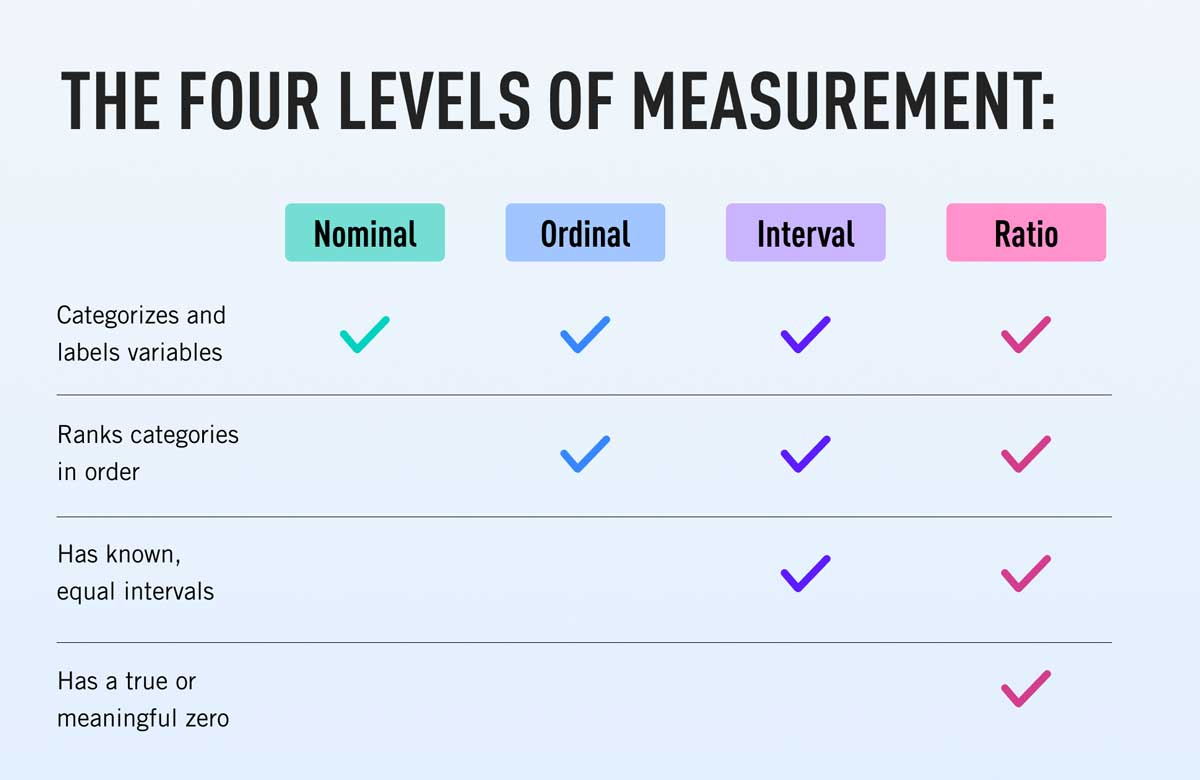
\includegraphics[width=1\linewidth,height=\textheight,keepaspectratio]{images/levels.jpg}
\caption{Levels of Measurement}
\end{figure}

\subsection*{Interval Level of Measurement}\label{interval-level-of-measurement}
\addcontentsline{toc}{subsection}{Interval Level of Measurement}

The \textbf{interval level} of measurement includes data with consistent intervals between values but lacks a true zero point. This means that while you can measure the differences between data points, the data does not allow for statements about absolute quantities. An example of interval data in media research is using a Likert scale, often employed in surveys to measure attitudes or opinions. On a scale from 1 to 5, where 1 represents strong disagreement, and 5 represents a strong agreement, the intervals between each point are equal, but there is no true zero---meaning that a score of 0 does not exist or represent ``no attitude.''

Interval data is particularly valuable in media studies when researchers aim to measure perceptions, attitudes, or responses with precision. Because the intervals between values are equal, you can calculate the mean or standard deviation of responses, which allows for more sophisticated statistical analysis than nominal or ordinal data. However, because interval data lacks a true zero point, it is important to avoid making statements about ratios or absolute quantities. For instance, you cannot say that a score of 4 on a Likert scale is ``twice as positive'' as a score of 2.

\subsection*{Ratio Level of Measurement}\label{ratio-level-of-measurement}
\addcontentsline{toc}{subsection}{Ratio Level of Measurement}

The \textbf{ratio level} of measurement is the most informative and precise, combining all the properties of the interval level with the addition of a true zero point. A true zero indicates the absence of the phenomenon being measured, allowing for meaningful statements about both absolute quantities and ratios. In mass media research, an example of ratio data could be the number of hours spent watching television per week. Since zero hours represent the complete absence of TV viewing, you can make comparisons such as, ``Person A watches twice as much TV as Person B.''

Ratio data is the most versatile and allows for the broadest range of statistical analyses. Researchers can calculate means, medians, variances, and ratios, providing a comprehensive understanding of the data. Ratio data is essential for studies that require precise measurement and comparison of quantities, such as time spent on media platforms, number of social media interactions, or advertising expenditures.

\section{Issues in Measurement}\label{issues-in-measurement}

Accurate and consistent measurement is critical to producing meaningful results in mass media research. However, several challenges can arise during the measurement process that can compromise the integrity of your findings. Among the most significant issues are \textbf{measurement error}, \textbf{validity}, and \textbf{reliability}. Understanding these concepts is essential for designing research that yields accurate and credible data.

\subsection*{Measurement Error}\label{measurement-error}
\addcontentsline{toc}{subsection}{Measurement Error}

\textbf{Measurement error} occurs when there is a discrepancy between the actual value of what is being measured and the observed value. This error can arise from various sources, and even minor inaccuracies can significantly affect a study's outcomes. Common sources of measurement error include respondent misinterpretations, data entry mistakes, and inconsistent data collection methods. For instance, if survey participants misunderstand a question, their answers may not accurately reflect their true thoughts or behaviors, leading to erroneous data. Likewise, the analysis may yield misleading conclusions if data is entered incorrectly into a database.

Consider a study examining the effectiveness of a media literacy program. If participants misunderstand a survey question about their media usage, their responses might not accurately reflect their true habits. This measurement error could skew the results, making it seem as though the media literacy program is more or less effective than it is. Recognizing and minimizing these errors is vital for ensuring the accuracy of research findings.

Minimizing measurement error begins with recognizing its potential sources. Clear, well-designed measurement tools can help reduce misunderstandings, while careful data entry and verification procedures can prevent errors during data processing. Ensuring consistent data collection methods across participants or conditions is equally important in reducing variability that might compromise the study's results.

\subsection*{Validity}\label{validity}
\addcontentsline{toc}{subsection}{Validity}

\textbf{Validity} refers to the extent to which a measurement tool accurately captures the intended concept. If a measurement lacks validity, it may not reflect the true nature of the concept under investigation, leading to incorrect conclusions. In social sciences and media research, \textbf{construct validity} is one of the most critical forms. Construct validity assesses whether the tool or scale genuinely measures the theoretical construct it aims to evaluate.

For example, imagine using a psychological scale in media studies to measure a concept like ``audience engagement.'' To determine whether the scale has strong construct validity, you must evaluate whether the questions truly capture all aspects of audience engagement. If the scale focuses too much on one dimension of engagement---such as how often a user clicks ``like'' on social media posts---while ignoring other important behaviors like commenting or sharing content, its validity would be compromised.

To ensure high construct validity, it's important to design measurement tools based on established theoretical frameworks carefully and to test those tools through pilot studies or existing literature. This process helps researchers verify that their tools accurately measure the concepts they intend to study, leading to more accurate and actionable research findings.

\begin{figure}
\centering
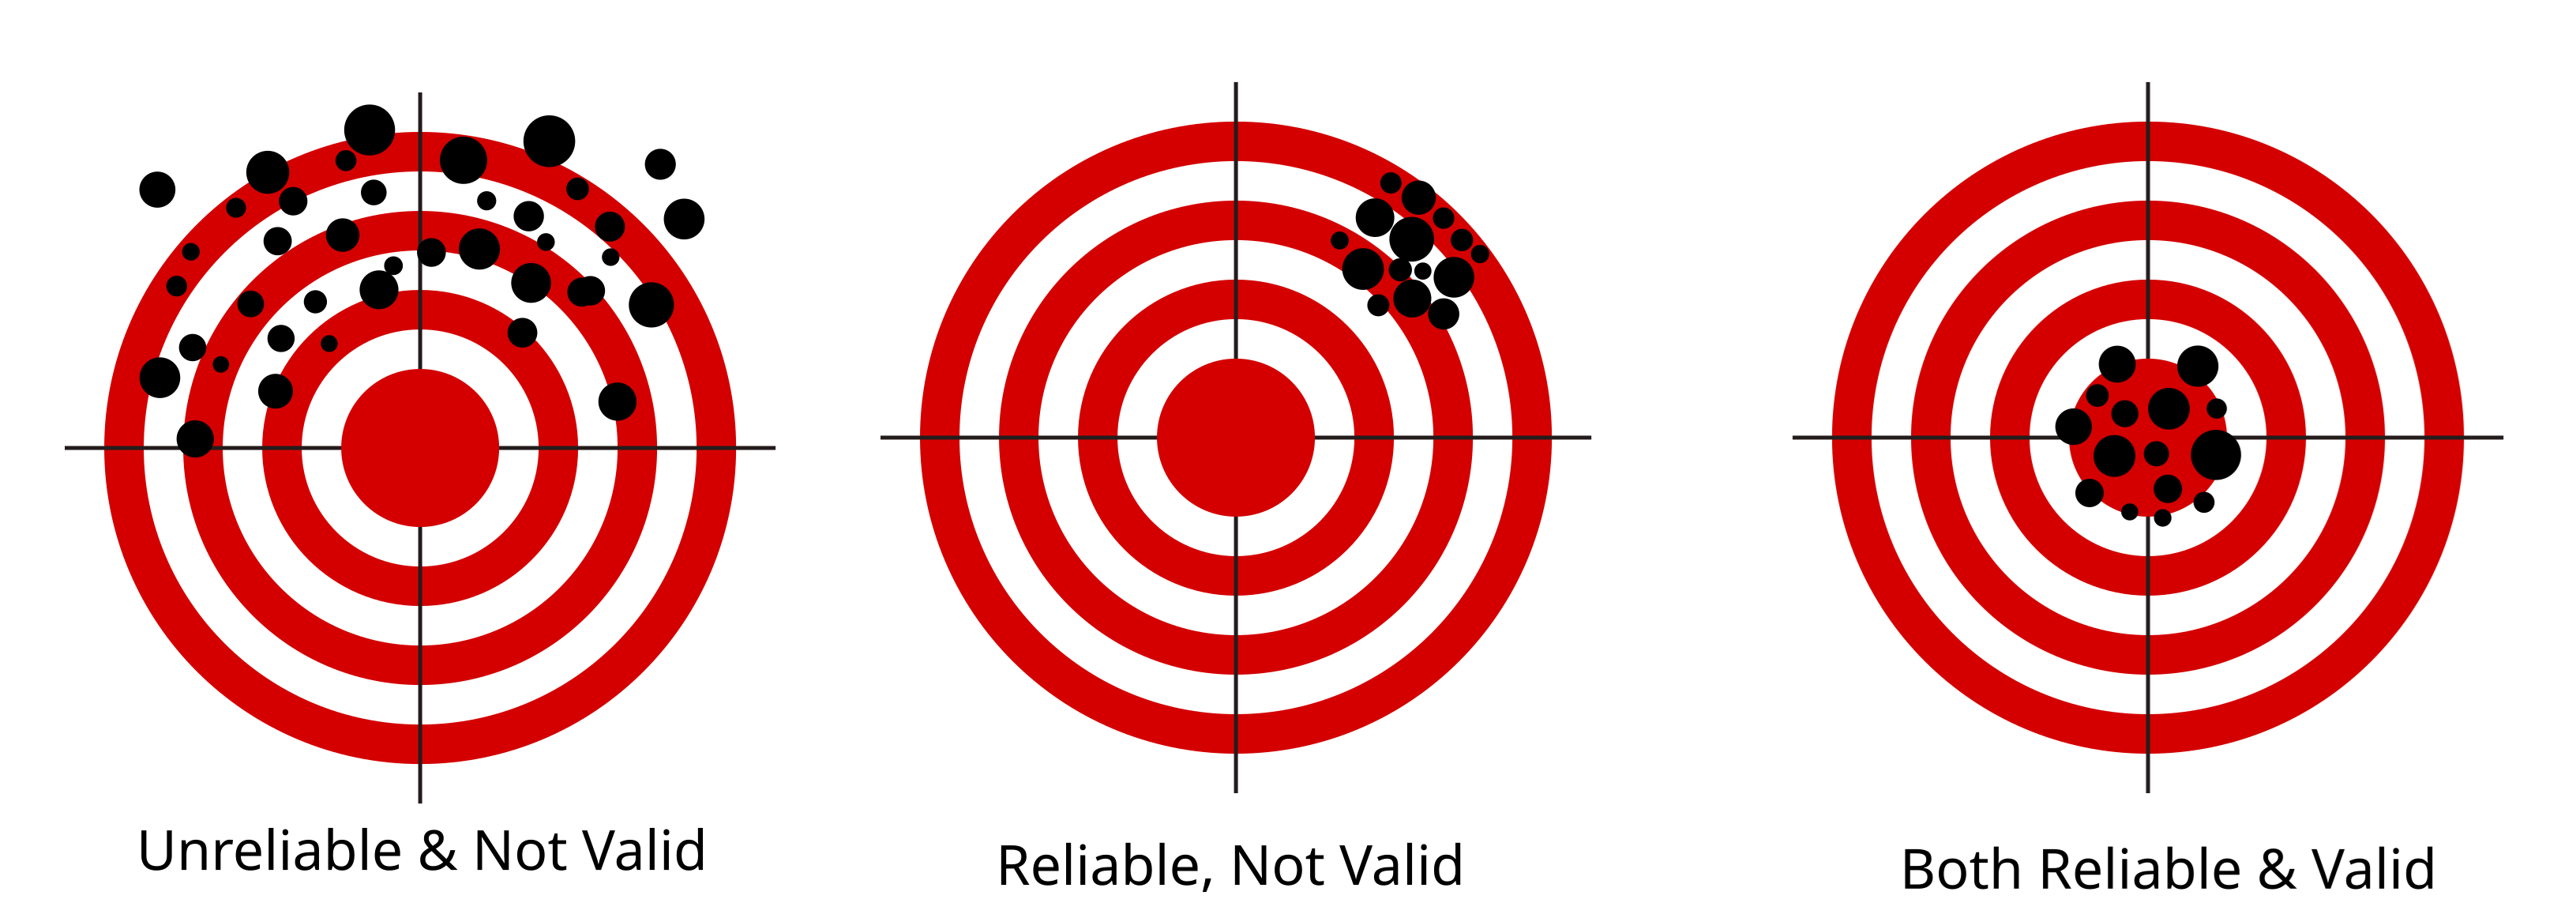
\includegraphics[width=1\linewidth,height=\textheight,keepaspectratio]{images/rel-val.png}
\caption{Reliable vs.~Valid}
\end{figure}

\subsection*{Reliability}\label{reliability}
\addcontentsline{toc}{subsection}{Reliability}

\textbf{Reliability} refers to the consistency of a measurement tool---its ability to produce the same results under the same conditions. A reliable tool will yield similar outcomes each time it is used, assuming that the measured phenomenon remains unchanged. Without reliability, even a valid measurement tool can lead to inconsistent and, thus, untrustworthy results.

For example, if a survey is designed to measure levels of audience engagement but produces vastly different results each time it is administered to the same group under similar conditions, the tool lacks reliability. As a result, it becomes difficult to draw meaningful conclusions from the data because the inconsistency casts doubt on whether the measurements truly reflect audience engagement.

Reliability is critical in mass media research because it ensures that findings are not the product of random fluctuations in measurement but are stable reflections of the studied phenomena. Several methods exist to assess reliability, including test-retest reliability (which evaluates whether the tool yields consistent results over time) and internal consistency (which checks if different parts of the measurement tool produce similar results).

\subsection*{The Relationship Between Validity and Reliability}\label{the-relationship-between-validity-and-reliability}
\addcontentsline{toc}{subsection}{The Relationship Between Validity and Reliability}

Recognizing that validity and reliability are related but distinct concepts is important. A measurement tool must be reliable and valid, as inconsistent results undermine any attempt to measure a construct accurately. However, a reliable tool is not necessarily valid. For instance, a scale might consistently measure something but not the concept it is intended to measure---thus, it is reliable but not valid.

In mass media research, achieving high reliability and high validity is critical to ensuring that your findings accurately reflect your study phenomena. Reliable tools provide stable measurements, while valid tools ensure that you measure the right constructs. Both are essential for producing research that contributes meaningfully to our understanding of media effects, behaviors, and perceptions.

\chapter{Communication Theories}\label{communication-theories}

\section{Agenda Setting Theory}\label{agenda-setting-theory}

Agenda setting theory is a communication theory that examines the relationship between the media and public opinion. Agenda Setting Theory examines the influence of the media in determining the importance placed on various public issues. This theory posits that by focusing on specific topics, the media shapes the public's perceptions of what is significant. The theory suggests that the media does not simply reflect public opinion, but rather shapes it by determining which issues are considered important. This is done by selecting and highlighting certain news stories over others, and by framing those stories in a particular way.

The theory was first proposed by Maxwell McCombs and Donald Shaw in their 1972 study of the 1968 US presidential election. They found that the media's coverage of the election had a significant impact on the public's perception of the relative importance of the issues. For example, the media focused heavily on the Vietnam War, which led to the public viewing this issue as more important than other issues, such as the economy.

Since then, agenda setting theory has been applied to a wide range of issues, including politics, social problems, and consumer products. The theory has been supported by a number of studies, but it is not without its critics. Some argue that the media does not have as much influence on public opinion as the theory suggests, and that other factors, such as personal experience and social interaction, are more important.

Despite these criticisms, agenda setting theory remains one of the most influential theories in mass communication. It has helped to explain how the media can shape public opinion, and it has implications for the way we think about the role of the media in society.

\textbf{Levels of agenda setting}

There are two levels of agenda setting:

\begin{itemize}
\item
  \textbf{First-level agenda setting}:~This level focuses on the media's ability to influence the salience of issues. Salience refers to the importance or prominence that people attach to an issue. The media can influence salience by selecting and highlighting certain issues over others.
\item
  \textbf{Second-level agenda setting}:~This level focuses on the media's ability to influence the public's perception of the attributes of an issue. This includes the causes, consequences, and solutions to the issue. The media can influence the public's perception of these attributes by the way they frame the issue in their news coverage.
\end{itemize}

\textbf{Factors affecting agenda setting}

There are a number of factors that can affect agenda setting, including:

\begin{itemize}
\item
  \textbf{The media's own agenda}: The media has its own agenda, which is influenced by a variety of factors, such as the ownership of the media outlet, the political climate, and the economic interests of the media.
\item
  \textbf{The public's agenda}: The public also has its own agenda, which is influenced by a variety of factors, such as personal experiences, social interaction, and the media.
\item
  \textbf{The political system}: The political system can also affect agenda setting by setting the agenda for public debate.
\item
  \textbf{The newsworthiness of the issue}: The newsworthiness of an issue is also a factor in agenda setting. Issues that are considered to be more newsworthy are more likely to be covered by the media.
\end{itemize}

\textbf{Conclusion}

Agenda setting theory is a complex and nuanced theory that has been the subject of much research and debate. However, it remains one of the most important theories in mass communication, and it has helped to explain how the media can shape public opinion.

\textbf{References}

\begin{itemize}
\item
  McCombs, M. E., \& Shaw, D. L. (1972). The agenda-setting function of mass media.~\emph{Public Opinion Quarterly, 36}(2), 176-187. \url{doi:10.1086/267990}
\item
  Dearing, J. W., \& Rogers, E. M. (1996). Agenda-setting. In M. B. Salwen \& D. W. Stacks (Eds.),~\emph{An introduction to mass communication theory}~(pp.~125-149). New York, NY: M. E. Sharpe.
\item
  Scheufele, D. A. (1999). Framing as a theory of media effects.~\emph{Journal of Communication, 49}(1), 103-122. \url{doi:10.1111/j.1460-2466.1999.tb02823.x}
\item
  Vliegenthart, R., \& Walgrave, S. (2008). The contingent nature of agenda setting: How political parties affect the salience of issues in government agendas.~\emph{Journal of Politics, 70}(4), 1111-1134. \url{doi:10.1017/S0022381608000363}
\item
  Chong, D., \& Druckman, J. N. (2010). Framing public opinion: How citizens react to elite communications.~\emph{Annual Review of Political Science, 13}, 103-126. \url{doi:10.1146/annurev.polisci.13.042009.102515}
\end{itemize}

\section{Cognitive Dissonance}\label{cognitive-dissonance}

Cognitive Dissonance describes the discomfort experienced when an individual holds contradictory beliefs or behaviors, prompting a drive to reduce the dissonance by changing attitudes or actions. This discomfort motivates the person to try to reduce the dissonance by changing one of the beliefs, changing their behavior, or finding a way to justify the inconsistency.

The theory of cognitive dissonance was first proposed by Leon Festinger in 1957. Festinger argued that people have a need for consistency in their thoughts, beliefs, and behaviors. When this consistency is threatened, people experience cognitive dissonance and are motivated to reduce it.

There are a number of ways that people can reduce cognitive dissonance. One way is to change one of the beliefs. For example, if a person believes that smoking is bad for their health, but they continue to smoke, they might start to believe that smoking is not as bad as they thought it was.

Another way to reduce cognitive dissonance is to change one's behavior. For example, if a person believes that they should eat healthy, but they continue to eat unhealthy foods, they might start to eat healthier foods.

Finally, people can also reduce cognitive dissonance by finding a way to justify the inconsistency. For example, a smoker might justify their smoking by saying that they enjoy it and that it helps them to relax.

Cognitive dissonance is a powerful motivator of human behavior. It can lead people to change their beliefs, their behaviors, or their justifications for their behavior. It can also lead to a number of other consequences, such as anxiety, stress, and depression.

Here are some examples of cognitive dissonance:

\begin{itemize}
\item
  A person who believes in saving money but spends all of their disposable income on unnecessary items.
\item
  A person who believes in being honest but cheats on their taxes.
\item
  A person who believes in eating healthy but eats junk food all the time.
\item
  A person who believes in animal rights but wears leather shoes.
\end{itemize}

These are just a few examples of how cognitive dissonance can manifest itself in our everyday lives. It is important to note that cognitive dissonance is not always negative. In some cases, it can motivate us to change our behavior for the better. For example, a person who experiences cognitive dissonance after smoking a cigarette might be more likely to quit smoking.

Cognitive dissonance is a complex phenomenon that has been studied by psychologists for many years. It is a powerful force that can have a significant impact on our thoughts, beliefs, and behaviors.

\textbf{References}

\begin{itemize}
\item
  Festinger, L. (1957).~\emph{A theory of cognitive dissonance}. Stanford, CA: Stanford University Press.
\item
  Cooper, J., \& Fazio, R. H. (1984). A new look at dissonance theory. In L. Berkowitz (Ed.),~\emph{Advances in experimental social psychology}~(Vol. 17, pp.~229-266).~New York, NY: Academic Press.
\item
  Harmon-Jones, E. (2002). Cognitive dissonance theory: Current status and controversies. In M. P. Zanna (Ed.),~\emph{Advances in experimental social psychology}~(Vol. 34, pp.~1-57). New York, NY: Academic Presss
\item
  Stone, J., \& Fernandez, G. (2016). Cognitive dissonance.~\emph{Current Opinion in Psychology, 11}, 100-105. \url{doi:10.1016/j.copsyc.2016.02.002}
\end{itemize}

\section{Cultivation Theory}\label{cultivation-theory}

Cultivation theory is a communication theory that examines the long-term effects of television viewing on viewers' conceptions of social reality. The Cultivation Theory suggests that long-term exposure to media content shapes viewers' perceptions of reality, aligning it more with the media's portrayal than actual societal norms. The theory was developed by George Gerbner and his colleagues at the University of Pennsylvania's Annenberg School for Communication in the 1960s.

Cultivation theory proposes that heavy television viewers come to see the world in a way that is consistent with the images and messages that they are repeatedly exposed to on television. This is because television is a powerful socializing agent that can shape our beliefs, attitudes, and values.

The theory has been supported by a number of studies, which have found that heavy television viewers are more likely to overestimate the likelihood of violence, crime, and danger in the world. They are also more likely to have a pessimistic view of human nature and to be fearful of strangers.

Cultivation theory has been criticized for being too simplistic and for failing to take into account other factors that can influence our perceptions of reality, such as personal experience and social interaction. However, the theory remains an important framework for understanding the effects of television on our lives.

Here are some of the key concepts of cultivation theory:

\begin{itemize}
\item
  \textbf{Symbolic environment}:~The world of television, as presented to viewers.
\item
  \textbf{Cultivation effect}:~The process by which heavy television viewing leads to viewers' perceptions of reality becoming more consistent with the images and messages presented on television.
\item
  \textbf{Mainstreaming}:~The tendency for heavy television viewers to come to share similar perceptions of reality, regardless of their demographic characteristics.
\item
  \textbf{Resonance}:~The process by which the cultivation effect is stronger for viewers who are already predisposed to believe the messages that are presented on television.
\end{itemize}

Cultivation theory has been applied to a wide range of topics, including violence, crime, fear, gender roles, and political attitudes. The theory has also been used to examine the effects of other media, such as the internet and video games.

Cultivation theory is a complex and nuanced theory that has been the subject of much research and debate. However, it remains one of the most important theories in mass communication, and it has helped to explain how television can shape our perceptions of reality.

\textbf{References}

\begin{itemize}
\item
  Gerbner, G., Gross, L., Morgan, M., \& Signorielli, N. (1986). Living with television: The dynamics of the cultivation process.~\emph{Communication Research, 13}(4), 373-398. \url{doi:10.1177/009365086013004001}
\item
  Morgan, M., \& Shanahan, J. (1997). Television and the cultivation of values: A 20-year assessment.~\emph{Communication Research, 24}(5), 367-399. \url{doi:10.1177/009365097024005001}
\item
  Shrum, L. J. (2004). Media consumption and perceptions of social reality: A cultivation perspective. In J. Bryant \& D. Zillmann (Eds.),~\emph{Media effects: Advances in theory and research}~(pp.~41-65). Mahwah, NJ: Lawrence Erlbaum Associates.
\item
  Potter, W. J. (2011).~\emph{Media literacy}~(9th ed.). Thousand Oaks, CA: Sage.
\end{itemize}

\section{Elaboration Likelihood Model}\label{elaboration-likelihood-model}

The elaboration likelihood model (ELM) is a dual-process theory of persuasion that was developed by Richard E. Petty and John Cacioppo in 1980. ELM outlines two pathways of persuasion: the central route, which involves thoughtful consideration of the arguments, and the peripheral route, which relies on superficial cues

The central route is a high-effort route to persuasion that involves carefully considering the message and evaluating the arguments presented. This route is more likely to be used when people are motivated and have the ability to think critically about the message.

The peripheral route is a low-effort route to persuasion that involves relying on superficial cues, such as the source of the message or the way it is presented. This route is more likely to be used when people are not motivated or do not have the ability to think critically about the message.

The ELM suggests that the effectiveness of a persuasive message depends on the route that is used. Messages that are processed through the central route are more likely to lead to lasting attitude change, while messages that are processed through the peripheral route are more likely to lead to temporary attitude change.

The ELM has been supported by a number of studies, and it has been used to explain a wide range of persuasion phenomena, such as the effects of advertising, political campaigns, and social movements.

Here are some of the key concepts of the ELM:

\begin{itemize}
\item
  \textbf{Elaboration}:~The amount of cognitive effort that is put into processing a message.
\item
  \textbf{Motivation}:~The desire to process a message in a thoughtful and unbiased way.
\item
  \textbf{Ability}:~The ability to process a message in a thoughtful and unbiased way.
\item
  \textbf{Peripheral cues}:~Superficial cues that are used to evaluate a message, such as the source of the message or the way it is presented.
\item
  \textbf{Central route to persuasion}:~A high-effort route to persuasion that involves carefully considering the message and evaluating the arguments presented.
\item
  \textbf{Peripheral route to persuasion}:~A low-effort route to persuasion that involves relying on superficial cues, such as the source of the message or the way it is presented.
\end{itemize}

The ELM is a complex and nuanced theory that has been the subject of much research and debate. However, it remains one of the most important theories in persuasion research, and it has helped to explain how people are persuaded by messages.

\textbf{References}

\begin{itemize}
\item
  Petty, R. E., \&~Cacioppo, J. T. (1986). The elaboration likelihood model of persuasion.~\emph{Advances in Experimental Social Psychology, 19}, 123-205. \url{doi:10.1016/S0065-2601(08)60214-2}
\item
  Petty,~R. E., \& Cacioppo, J. T. (1996).~\emph{Attitude change: Classic and contemporary approaches}. New York, NY: McGraw-Hill.
\item
  Chaiken, S. (1980). Heuristic versus systematic processing of persuasive messages: Evidence of two routes to persuasion. \_In J. T. Cacioppo \& R. E. Petty (Eds.),~\emph{Social cognition: The Ontario symposium on personality and social psychology}~(Vol. 1, pp.~212-252). Hillsdale, NJ: Erlbaum.
\end{itemize}

\section{Framing Theory}\label{framing-theory}

Framing theory is a communication theory that examines how the way an issue is presented can affect how people understand and respond to it. The theory was first proposed by Erving Goffman in 1974, and it has been used to explain a wide range of phenomena, such as the effects of news coverage on public opinion, the impact of advertising on consumer behavior, and the role of social movements in shaping public discourse.

Framing theory suggests that the way an issue is presented can shape how people think about it by influencing the following:

\begin{itemize}
\item
  \textbf{The salience of the issue}:~The extent to which the issue is noticed and remembered.
\item
  \textbf{The definition of the issue}:~The way the issue is understood and interpreted.
\item
  \textbf{The causal attributions}:~The reasons that are given for the issue.
\item
  \textbf{The moral implications}:~The ethical or moral dimensions of the issue.
\item
  \textbf{The emotional response}:~The feelings that are evoked by the issue.
\end{itemize}

Framing theory has been supported by a number of studies, which have found that the way an issue is framed can have a significant impact on how people think about it and respond to it. For example, studies have shown that the way news stories about crime are framed can affect people's fear of crime, and the way advertising is framed can affect people's purchase decisions.

Framing theory is a complex and nuanced theory that has been the subject of much research and debate. However, it remains an important framework for understanding how the way we communicate about issues can shape how people think about them.

Here are some of the key concepts of framing theory:

\begin{itemize}
\item
  \textbf{Frame}:~A way of presenting an issue that highlights certain aspects of the issue and obscures others.
\item
  \textbf{Framing effects}:~The ways in which the way an issue is framed can affect how people think about it and respond to it.
\item
  \textbf{Framing bias}:~The tendency for people to be more persuaded by messages that are framed in a way that is consistent with their existing beliefs and attitudes.
\item
  \textbf{Framing strategies}:~The techniques that are used to frame issues, such as the use of language, images, and metaphors.
\end{itemize}

Framing theory has been applied to a wide range of topics, including politics, health, the environment, and social justice. The theory has also been used to examine the effects of different media, such as news, advertising, and social media.

Framing theory is a powerful tool for understanding how the way we communicate about issues can shape how people think about them. By understanding how framing works, we can be more mindful of the ways in which our own communication can influence others.

\textbf{References}

\begin{itemize}
\item
  Entman, R. M. (1993). Framing: Toward clarification of a fractured paradigm.~\emph{Journal of Communication, 43}(4), 51-58. \url{doi:10.1111/j.1460-2466.1993.tb01304.x}
\item
  Scheufele, D. A. (1999). Framing as a theory of media effects.~\emph{Journal of Communication, 49}(1), 103-122. \url{doi:10.1111/j.1460-2466.1999.tb02823.x}
\item
  Chong, D., \& Druckman, J. N. (2010). Framing public opinion: How citizens react to elite communications.~\emph{Annual Review of Political Science, 13}, 103-126. \url{doi:10.1146/annurev.polisci.13.042009.102515}
\end{itemize}

\section{Gatekeeping Theory}\label{gatekeeping-theory}

Gatekeeping theory is a communication theory that examines how decisions are made about what news stories get covered and how they are presented. The theory was first proposed by Kurt Lewin in 1947, and it has been used to explain a wide range of phenomena, such as the effects of news coverage on public opinion, the impact of media bias, and the role of journalists in shaping public discourse.

Gatekeeping theory suggests that there are a number of factors that can influence the news selection process, including:

\begin{itemize}
\item
  \textbf{The gatekeepers}:~The people who make decisions about what news stories get covered and how they are presented.
\item
  \textbf{The news values}:~The criteria that are used to determine which news stories are newsworthy.
\item
  \textbf{The media environment}:~The economic, political, and social factors that shape the media.
\item
  \textbf{The audience}:~The people who consume news.
\end{itemize}

Gatekeeping theory has been supported by a number of studies, which have found that the news selection process is often influenced by the gatekeepers' personal biases, the news values of the media organization, and the political and economic climate.

For example, studies have shown that journalists are more likely to cover stories that are consistent with their own political beliefs, and that news organizations are more likely to cover stories that are seen as being in the public interest or that are likely to attract a large audience.

Gatekeeping theory is a complex and nuanced theory that has been the subject of much research and debate. However, it remains an important framework for understanding how decisions are made about what news stories get covered and how they are presented.

Here are some of the key concepts of gatekeeping theory:

\begin{itemize}
\item
  \textbf{Gatekeeper}:~A person who makes decisions about what news stories get covered and how they are presented.
\item
  \textbf{News values}:~The criteria that are used to determine which news stories are newsworthy.
\item
  \textbf{Media environment}:~The economic, political, and social factors that shape the media.
\item
  \textbf{Audience}:~The people who consume news.
\item
  \textbf{Personal bias}:~The personal beliefs and opinions of the gatekeeper.
\item
  \textbf{News organization}:~The media outlet where the gatekeeper works.
\item
  \textbf{Public interest}:~The perceived benefit to the public of covering a particular news story.
\item
  \textbf{Large audience}:~The perceived potential for a news story to attract a large number of viewers or readers.
\end{itemize}

Gatekeeping theory has been applied to a wide range of topics, including politics, health, the environment, and social justice. The theory has also been used to examine the effects of different media, such as news, advertising, and social media.

Gatekeeping theory is a powerful tool for understanding how decisions are made about what news stories get covered and how they are presented. By understanding how gatekeeping works, we can be more mindful of the ways in which our own news consumption can be influenced.

\textbf{References}

\begin{itemize}
\item
  Lewin, K. (1947).~Frontiers in group dynamics: Concept, method and reality in social science; social equilibria and social change.~\emph{Human Relations,~1}(2), 5-41. \url{doi:10.1177/001872674700100201}
\item
  Shoemaker, P. J., \&~Reese, S. D. (1996).~\emph{Mediating the message: Theories of influences on mass media content}~(2nd ed.). New York, NY: Longman.
\item
  Tuchman, G. (1978).~\emph{Making news: A study in the construction of reality}. New York, NY: Free Press.
\end{itemize}

\section{Hyperpersonal Model}\label{hyperpersonal-model}

The hyperpersonal model is a communication theory that examines how computer-mediated communication (CMC) can create more personal and intimate relationships than traditional face-to-face (FtF) communication. The theory was proposed by Joseph Walther in 1992, and it has been used to explain a wide range of phenomena, such as the development of online relationships, the impact of CMC on social interaction, and the role of CMC in shaping our self-presentation.

The hyperpersonal model suggests that CMC can create more personal and intimate relationships than FtF communication because it offers a number of advantages, including:

\begin{itemize}
\item
  \textbf{Attribution ambiguity}:~The sender's physical appearance and nonverbal cues are not available in CMC, which allows the receiver to fill in the gaps with their own interpretations.
\item
  \textbf{Control over self-presentation}:~CMC allows users to control their self-presentation more than FtF communication, which can lead to more favorable impressions.
\item
  \textbf{Attribution confidence}:~CMC users are more likely to believe that they have accurate information about the other person, which can lead to more trust and intimacy.
\item
  \textbf{Interactivity}:~CMC is more interactive than traditional mass media, which allows for more communication and feedback between the sender and receiver.
\end{itemize}

The hyperpersonal model has been supported by a number of studies, which have found that CMC users often report feeling more connected and intimate with their online partners than they do with their FtF partners. For example, one study found that CMC users were more likely to disclose personal information to their online partners than they were to their FtF partners.

However, the hyperpersonal model has also been criticized for being too simplistic and for failing to take into account the role of other factors, such as the individual's personality and the relationship context. Nevertheless, the hyperpersonal model remains an important framework for understanding how CMC can create more personal and intimate relationships than traditional FtF communication.

Here are some of the key concepts of the hyperpersonal model:

\begin{itemize}
\item
  \textbf{Attribution ambiguity}:~The lack of physical cues in CMC can lead to ambiguity about the sender's intentions and personality.
\item
  \textbf{Control over self-presentation}:~CMC allows users to control how they are perceived by others.
\item
  \textbf{Attribution confidence}:~CMC users are more likely to believe that they have accurate information about the other person.
\item
  \textbf{Interactivity}:~CMC allows for more communication and feedback between the sender and receiver.
\item
  \textbf{Hyperpersonal communication}:~Communication that is more personal and intimate than traditional face-to-face communication.
\end{itemize}

The hyperpersonal model has been applied to a wide range of topics, including online dating, online gaming, and social media. The theory has also been used to examine the effects of different CMC technologies, such as email, instant messaging, and social networking sites.

The hyperpersonal model is a powerful tool for understanding how CMC can create more personal and intimate relationships than traditional FtF communication. By understanding how the hyperpersonal model works, we can be more mindful of the ways in which our own CMC interactions can be shaped.

\textbf{References}

\begin{itemize}
\item
  Walther, J. B. (1992). Interpersonal effects in computer-mediated communication:~A relational perspective.~\emph{Communication Research, 19}(1), 52-90.~\url{doi:10.1177/009365092019001003}
\item
  Walther, J. B. (1996). Computer-mediated communication: Impersonal, interpersonal, and hyperpersonal interaction.~\emph{Communication Research, 23}(1), 3-43. \url{doi:10.1177/009365096023001001}
\item
  Walther,~J. B. (2007). Selective self-presentation in computer-mediated communication: Hyperpersonal dimensions of technology, language, and~the self.~\emph{Computers in Human Behavior, 23}(5), 2637-2653. \url{doi:10.1016/j.chb.2005.10.014}
\end{itemize}

\section{Knowledge Gap Hypothesis}\label{knowledge-gap-hypothesis}

The knowledge gap hypothesis (KGH) is a communication theory that predicts that the gap in knowledge between the informed and the uninformed will widen over time, rather than close, as a result of mass communication. The theory was first proposed by Philip J. Tichenor, George A. Donohue, and Clarice N. Olien in 1970, and it has been used to explain a wide range of phenomena, such as the effects of news coverage on public opinion, the impact of educational campaigns, and the role of the media in shaping social inequality.

The KGH suggests that the gap in knowledge between the informed and the uninformed will widen over time because of the following factors:

\begin{itemize}
\item
  \textbf{Differential access to information}:~People with higher socioeconomic status (SES) are more likely to have access to information, such as through education, the media, and social networks.
\item
  \textbf{Differential motivation to learn}:~People with higher SES are more likely to be motivated to learn about new information, such as because they are more likely to be involved in civic activities or to have a need for the information.
\item
  \textbf{Differential ability to understand information}:~People with higher SES are more likely to be able to understand and retain new information, such as because they have more cognitive resources or because they are more familiar with the language and concepts used in the information.
\end{itemize}

The KGH has been supported by a number of studies, which have found that the gap in knowledge between the informed and the uninformed does indeed widen over time. For example, one study found that the gap in knowledge about climate change between people with high and low levels of education widened over a period of 15 years.

However, the KGH has also been criticized for being too simplistic and for failing to take into account the role of other factors, such as the individual's motivation and the nature of the information. Nevertheless, the KGH remains an important framework for understanding how mass communication can contribute to social inequality.

Here are some of the key concepts of the knowledge gap hypothesis:

\begin{itemize}
\item
  \textbf{Knowledge gap}:~The difference in knowledge between the informed and the uninformed.
\item
  \textbf{Mass communication}:~The process of sending messages to a large audience through the media.
\item
  \textbf{Socioeconomic status (SES)}:~A measure of a person's social and economic position, such as their income, education, and occupation.
\item
  \textbf{Differential access to information}:~The unequal distribution of information among different groups of people.
\item
  \textbf{Differential motivation to learn}:~The different levels of motivation that people have to learn new information.
\item
  \textbf{Differential ability to understand information}:~The different levels of ability that people have to understand and retain new information.
\end{itemize}

The KGH has been applied to a wide range of topics, such as public health, education, and politics. The theory has also been used to examine the effects of different media, such as news, advertising, and social media.

The KGH is a powerful tool for understanding how mass communication can contribute to social inequality. By understanding how the KGH works, we can be more mindful of the ways in which our own communication can help to widen or narrow the knowledge gap.

\textbf{References}

\begin{itemize}
\item
  Tichenor, P. J., Donohue, G. A., \& Olien, C. N. (1970). Mass media flow and differential growth in knowledge.~\emph{Public Opinion Quarterly, 34}(2),~159-170. \url{doi:10.1086/267856}
\item
  Viswanath, K., \& Finnegan, J. R. (1996). The knowledge gap hypothesis: Twenty-five years later.~\emph{Communication Research, 23}(5), 559-587. \url{doi:10.1177/009365096023005003}
\item
  Weimann, G. (1994). The influentials: People who influence people. New York, NY: Transaction Publishers.
\end{itemize}

\section{Online Disinhibition Effect}\label{online-disinhibition-effect}

The online disinhibition effect (ODE) is a phenomenon that occurs when people are more likely to say or do things online that they would not say or do in person. The ODE can be attributed to a number of factors, including:

\begin{itemize}
\item
  \textbf{Anonymity}:~When people are anonymous, they are less likely to feel inhibited by social conventions or norms.
\item
  \textbf{Immediacy}:~Online communication is often more immediate than face-to-face communication, which can lead to people saying things without thinking them through.
\item
  \textbf{Absence of cues}:~Online communication lacks many of the social cues that are present in face-to-face communication, such as body language and tone of voice. This can make it difficult to interpret messages and can lead to misunderstandings.
\item
  \textbf{Disinhibition}:~The ODE can also be attributed to a personality trait known as disinhibition, which is the tendency to act without thinking about the consequences.
\end{itemize}

The ODE can have both positive and negative consequences. On the one hand, it can allow people to be more honest and open than they would be in person. This can be beneficial for communication and relationships. On the other hand, the ODE can also lead to cyberbullying, trolling, and other forms of online harassment.

Here are some of the key concepts of the online disinhibition effect:

\begin{itemize}
\item
  \textbf{Anonymity}:~The state of being unknown or unidentifiable.
\item
  \textbf{Immediacy}:~The quality of being happening or occurring at the same time.
\item
  \textbf{Absence of cues}:~The lack of social cues, such as body language and tone of voice, in online communication.
\item
  \textbf{Disinhibition}:~The tendency to act without thinking about the consequences.
\item
  \textbf{Online disinhibition effect (ODE)}:~The phenomenon that occurs when people are more likely to say or do things online that they would not say or do in person.
\end{itemize}

The ODE has been studied by psychologists and communication scholars for many years. There is still much that we do not know about the ODE, but it is a phenomenon that is important to understand in order to use online communication safely and effectively.

Here are some of the ways to mitigate the negative effects of the ODE:

\begin{itemize}
\item
  \textbf{Be aware of the ODE}:~The first step to mitigating the negative effects of the ODE is to be aware of it. Once you are aware of the ODE, you can start to think about how it might be affecting your online behavior.
\item
  \textbf{Be mindful of your audience}:~When you are communicating online, it is important to be mindful of your audience. Remember that the people you are communicating with may not be who they say they are.
\item
  \textbf{Think before you post}:~Before you post anything online, take a moment to think about what you are saying and how it might be interpreted.
\item
  \textbf{Use appropriate language}:~Be mindful of the language you use online. Avoid using language that could be offensive or hurtful.
\item
  \textbf{Be respectful}:~Always be respectful of others, even if you disagree with them.
\end{itemize}

The ODE is a complex phenomenon, but by being aware of it and taking steps to mitigate its negative effects, we can use online communication safely and effectively.

\textbf{References}

\begin{itemize}
\item
  Suler, J. (2004). The online disinhibition effect.~\emph{Cyberpsychology \& Behavior, 7}(3), 321-326. \url{doi:10.1089/1094931041291295}
\item
  Joinson, A. N. (2001). Self-disclosure in computer-mediated communication: The role of self-awareness and privacy concerns.~\emph{European Journal of Social Psychology, 31}(2), 177-192. \url{doi:10.1002/ejsp.141}
\item
  Postmes, T., Spears, R., \& Lea, M. (2000). The social psychology of computer-mediated communication.~\emph{Annual Review of Psychology, 51}, 669-703. \url{doi:10.1146/annurev.psych.51.1.669}
\item
  Tanis, M. (2008). Online disinhibition: Implications for understanding computer-mediated communication.~\emph{Computers in Human Behavior, 24}(6), 2253-2260. \url{doi:10.1016/j.chb.2008.02.007}
\item
  McKenna, K. Y. A., \& Bargh, J. A. (1998). In-group affiliation and computer-mediated communication: Group versus individual identity salience.~\emph{Personality and Social Psychology Bulletin, 24}(10), 1095-1105. \url{doi:10.1177/01461672982410006}
\end{itemize}

\section{Parasocial Interaction}\label{parasocial-interaction}

Parasocial Interaction Theory (PSI) describes the phenomenon where individuals form one-sided relationships with media personalities, interacting with them as if they were part of their social circle. The term was coined by Donald Horton and Richard Wohl in 1956, who defined it as ``the perception of the performer-audience relationship as involving mutual intimacy.''

PSI can occur in any medium where there is a one-way flow of communication, such as television, radio, and the internet. It is most likely to occur when the media persona is perceived as being attractive, likable, and trustworthy.

There are a number of factors that can contribute to PSI, including:

\begin{itemize}
\item
  \textbf{The amount of exposure}:~The more exposure a person has to a media persona, the more likely they are to develop a parasocial relationship with that persona.
\item
  \textbf{The perceived similarity}:~People are more likely to develop parasocial relationships with media personas who they perceive as being similar to themselves.
\item
  \textbf{The perceived intimacy}:~The more intimate the relationship between the media persona and the viewer or listener is perceived to be, the more likely PSI is to occur.
\end{itemize}

PSI can have both positive and negative consequences. On the one hand, it can provide comfort and companionship for people who are lonely or isolated. On the other hand, it can lead to unrealistic expectations about relationships and can make it difficult to form real-world relationships.

Here are some of the key concepts of parasocial interaction:

\begin{itemize}
\item
  \textbf{Parasocial interaction (PSI)}:~The illusion of a close relationship between a media persona and a viewer or listener.
\item
  \textbf{Media persona}:~A person who is presented to an audience through a media medium.
\item
  \textbf{Viewer or listener}:~A person who consumes media content.
\item
  \textbf{Mutual intimacy}:~The perception that two people share a close and personal relationship.
\item
  \textbf{Unrealistic expectations}:~Expectations that are not based on reality.
\end{itemize}

PSI has been studied by psychologists and communication scholars for many years. There is still much that we do not know about PSI, but it is a phenomenon that is important to understand in order to understand the effects of media on people.

Here are some of the key citations in APA 7th for parasocial interaction:

\begin{itemize}
\item
  Horton,~D., \& Wohl, R. R. (1956). Mass communication and para-social interaction: Observations on intimacy at a distance.~\emph{Psychiatry, 19}(3), 215-229.~\url{doi:10.1176/ps.19.3.215}
\item
  Rubin, A. M. (1977). Relationships between television viewing patterns and social behaviors.~\emph{Communication Research, 4}(1), 19-51. \url{doi:10.1177/009365077004001002}
\item
  Perse, E. M. (1990). Media involvement and other predictors of audience response to televised political advertisements.~\emph{Communication Research, 17}(1), 155-177. \url{doi:10.1177/009365090017001007}
\item
  Giles, D., \& Maltby, J. (2015). The parasocial relationship: A critical review of the literature.~\emph{Communication Research, 42}(6), 752-777. \url{doi:10.1177/0093650214544163}
\item
  Rubin, A. M., \& Rubin, R. B. (2015).~\emph{Communication research: Approaches and methods}~(7th ed.). Boston, MA: Pearson.
\end{itemize}

\section{Social Learning Theory}\label{social-learning-theory}

Social learning theory is a psychological theory that explains how people learn new behaviors by observing and modeling the behaviors of others. The theory was developed by Albert Bandura in the 1960s, and it has been used to explain a wide range of phenomena, such as the development of aggression, the acquisition of prosocial behaviors, and the impact of media on behavior.

Social learning theory is based on the following assumptions:

\begin{itemize}
\item
  People learn by observing and modeling the behaviors of others.~This is known as observational learning.
\item
  The learning process is influenced by a number of factors, including attention, retention, reproduction, and reinforcement.
\item
  People are more likely to learn behaviors that are rewarded or reinforced.
\item
  People are also more likely to learn behaviors that are performed by people they admire or respect.
\end{itemize}

Social learning theory has been supported by a number of studies, which have found that people are more likely to imitate the behaviors of others when they are paying attention to those behaviors, when they can remember those behaviors, and when they are rewarded for imitating those behaviors.

Social learning theory has been applied to a wide range of topics, such as aggression, prosocial behavior, and the impact of media on behavior. For example, studies have found that children who are exposed to violence in the media are more likely to behave aggressively themselves. This is because they are learning that violence is an acceptable way to resolve conflict.

Social learning theory is a powerful tool for understanding how people learn new behaviors. By understanding the principles of social learning theory, we can better understand how to promote positive behaviors and prevent negative behaviors.

Here are some of the key concepts of social learning theory:

\begin{itemize}
\item
  \textbf{Observational learning}:~The process of learning new behaviors by observing and modeling the behaviors of others.
\item
  \textbf{Attention}:~The process of paying attention to the behaviors of others.
\item
  \textbf{Retention}:~The process of remembering the behaviors of others.
\item
  \textbf{Reproduction}:~The process of imitating the behaviors of others.
\item
  \textbf{Reinforcement}:~A consequence that increases the likelihood of a behavior being repeated.
\end{itemize}

Here are some of the key citations in APA 7th for social learning theory:

\begin{itemize}
\item
  Bandura, A. (1977).~\emph{Social learning theory}. Englewood Cliffs, NJ: Prentice-Hall.
\item
  Bandura, A. (1986). Social foundations of thought and action: A social cognitive theory. Englewood Cliffs, NJ: Prentice-Hall.
\item
  Bandura, A. (1997).~\emph{Self-efficacy: The exercise of control}. New York,~NY:~Freeman.
\item
  Bandura, A. (2001). Social cognitive theory: An agentic perspective.~\emph{Annual Review of Psychology, 52}, 1-26. \url{doi:10.1146/annurev.psych.52.1.1}
\item
  Bandura, A. (2006).~\emph{Social cognitive theory of mass communication}. Thousand Oaks, CA: Sage.
\end{itemize}

\section{Social Constructionism}\label{social-constructionism}

Social constructionism is a theoretical perspective that emphasizes the role of social interaction in shaping our understanding of the world. The theory was developed by a number of scholars, including Peter Berger and Thomas Luckmann, who argued that knowledge is not objective or preexisting, but is instead created and negotiated through social interaction.

Social constructionism is based on the following assumptions:

\begin{itemize}
\item
  \textbf{There is no objective reality}.~What we perceive as reality is a social construct, created and negotiated through interaction with others.
\item
  \textbf{Knowledge is created through language}.~We use language to communicate our experiences and understandings of the world, and these shared understandings become the basis for knowledge.
\item
  \textbf{Knowledge is constantly changing}.~As we interact with others and our experiences change, our understanding of the world also changes.
\end{itemize}

Social constructionism has been applied to a wide range of topics, including gender, race, and ethnicity. For example, social constructionists argue that gender is not a biological reality, but is instead a social construct that is created and negotiated through interaction. They point out that the way we think about gender varies across cultures and historical periods, which suggests that it is not an objective reality.

Social constructionism has been criticized for being relativist, meaning that it suggests that there is no such thing as truth. However, social constructionists argue that this does not mean that anything goes. They believe that there are still shared understandings of the world that are worth striving for, even if these understandings are constantly changing.

Here are some of the key concepts of social constructionism:

\begin{itemize}
\item
  \textbf{Social constructivism}:~A theoretical perspective that emphasizes the role of social interaction in shaping our understanding of the world.
\item
  \textbf{Knowledge}:~A shared understanding of the world that is created and negotiated through social interaction.
\item
  \textbf{Language}:~The primary tool that we use to communicate our experiences and understandings of the world.
\item
  \textbf{Reality}:~A social construct that is created and negotiated through social interaction.
\end{itemize}

Here are some of the key citations in APA 7th for social constructionism:

\begin{itemize}
\item
  Berger, P., \& Luckmann, T. (1966).~\emph{The social construction of reality}. Garden City, NY: Anchor Books.
\item
  Gergen, K. J. (1999).~\emph{An invitation to social construction}. Thousand Oaks, CA: Sage.
\item
  Burr, V. (2015).~\emph{Social constructionism}~(4th ed.). London, UK: Routledge.
\item
  Hacking, I. (1999).~\emph{The social construction of what?}~Cambridge, MA: Harvard University Press.
\item
  Wood, J. (2013).~\emph{Social psychology}~(13th ed.). Boston, MA: Wadsworth.
\end{itemize}

\section{Social Exchange Theory}\label{social-exchange-theory}

Social exchange theory is a sociological and psychological theory that explains how people interact with each other based on the costs and rewards of those interactions. The theory was developed by George Homans in the 1950s, and it has been used to explain a wide range of phenomena, such as the formation of relationships, the development of norms, and the maintenance of social order.

Social exchange theory is based on the following assumptions:

\begin{itemize}
\item
  People are motivated to maximize their rewards and minimize their costs.
\item
  People make decisions about their interactions based on the perceived costs and rewards of those interactions.
\item
  People's expectations about the costs and rewards of an interaction can be influenced by their past experiences, their social norms, and their individual goals.
\end{itemize}

Social exchange theory has been supported by a number of studies, which have found that people are more likely to interact with others who they perceive as being rewarding. For example, studies have found that people are more likely to be friends with people who are similar to them, who are attractive, and who are kind and supportive.

Social exchange theory has been applied to a wide range of topics, such as interpersonal relationships, group dynamics, and organizations. For example, social exchange theory can be used to explain why people stay in relationships that are not satisfying, why people conform to social norms, and why people cooperate with each other in organizations.

Social exchange theory is a powerful tool for understanding how people interact with each other. By understanding the principles of social exchange theory, we can better understand why people behave the way they do and how to influence their behavior.

Here are some of the key concepts of social exchange theory:

\begin{itemize}
\item
  \textbf{Cost}:~The negative consequences of an interaction.
\item
  \textbf{Reward}:~The positive consequences of an interaction.
\item
  \textbf{Expectation}:~The perceived likelihood that an interaction will result in a particular outcome.
\item
  \textbf{Norm}:~A shared expectation about how people should behave in a particular situation.
\item
  \textbf{Goal}:~A desired outcome that a person is trying to achieve.
\end{itemize}

Here are some of the key citations in APA 7th for social exchange theory:

\begin{itemize}
\item
  Homans, G. C. (1958).~\emph{Social behavior as exchange}. American Journal of Sociology, 63(6), 597-606. \url{doi:10.1086/266639}
\item
  Blau, P. M. (1964).~\emph{Exchange and power in social life}. New York, NY: Wiley.
\item
  Thibaut, J. W., \& Kelley, H. H. (1959).~\emph{The social psychology of groups}. New York, NY: Wiley.
\item
  Molm, L. D. (2003).~\emph{Theorizing social exchange: An overview}. Boulder, CO: Paradigm Publishers.
\item
  Lawler, E. J., \& Yoon, J. (1993). Power and exchange: Asymmetries in social exchange. American Sociological Review, 58(5), 516-531. \url{doi:10.2307/2096313}
\end{itemize}

\section{Social Identity Theory}\label{social-identity-theory}

Social identity theory is a social psychology theory that explains how people categorize themselves and others into groups, and how these group memberships affect their self-concept and behavior. The theory was developed by Henri Tajfel and John Turner in the 1970s, and it has been used to explain a wide range of phenomena, such as prejudice, discrimination, and intergroup conflict.

Social identity theory is based on the following assumptions:

\begin{itemize}
\item
  People have a fundamental need to belong to groups.
\item
  People define themselves in terms of their group memberships.
\item
  People are motivated to maintain a positive social identity, which is the perception that their own group is positive and valuable.
\item
  People make comparisons between their own group and other groups.
\item
  These comparisons can lead to positive in-group bias, where people favor their own group over other groups.
\end{itemize}

Social identity theory has been supported by a number of studies, which have found that people are more likely to favor their own group over other groups, even when the groups are not objectively different. For example, studies have found that people are more likely to help members of their own group than members of other groups, and they are more likely to view members of their own group more favorably than members of other groups.

Social identity theory has been applied to a wide range of topics, such as prejudice, discrimination, and intergroup conflict. For example, social identity theory can be used to explain why people are prejudiced against members of other groups, why people discriminate against members of other groups, and why intergroup conflict occurs.

Social identity theory is a powerful tool for understanding how people's group memberships affect their self-concept and behavior. By understanding the principles of social identity theory, we can better understand why people behave the way they do in intergroup contexts.

Here are some of the key concepts of social identity theory:

\begin{itemize}
\item
  \textbf{Social identity}:~The part of a person's self-concept that is derived from their membership in a social group.
\item
  \textbf{In-group}:~The group to which a person belongs.
\item
  \textbf{Out-group}:~A group to which a person does not belong.
\item
  \textbf{Positive in-group bias}:~The tendency to favor one's own group over other groups.
\item
  \textbf{Intergroup conflict}:~Hostile interactions between groups.
\end{itemize}

Here are some of the key citations in APA 7th for social identity theory:

\begin{itemize}
\item
  Tajfel, H., \& Turner, J. C. (1979). An integrative theory of intergroup conflict. In W. G. Austin \&~S. Worchel (Eds.),~\emph{The social psychology of intergroup relations}~(pp.~33-47). Monterey, CA: Brooks/Cole.
\item
  Turner, J. C. (1982).~\emph{Towards a cognitive~theory of social identity and group behavior}. In H. Tajfel (Ed.),~\emph{Social identity and intergroup relations}~(pp.~27-52). Cambridge, MA: Cambridge University Press.
\item
  Hogg, M. A. (2006).~\emph{Social identity theory}. New York, NY: Psychology Press.
\item
  Abrams, D., \& Hogg, M. A. (2010).~\emph{Social identity and social cognition}~(2nd ed.). New York, NY: Psychology Press.
\item
  Smith, J. R. (2012).~\emph{Social identity theory: Key readings}. London, UK: Sage.
\end{itemize}

\section{Social Information Processing Theory}\label{social-information-processing-theory}

Social information processing theory (SIP) is a cognitive theory of social interaction that was developed by Kenneth Dodge in the 1980s. The theory explains how people make sense of social interactions and how these interpretations influence their behavior.

SIP is based on the following assumptions:

\begin{itemize}
\item
  People are active processors of social information.
\item
  They attend to and interpret cues from the social environment.
\item
  They generate and evaluate possible responses to these cues.
\item
  They choose the response that they believe will be most successful.
\end{itemize}

SIP has been supported by a number of studies, which have found that people do indeed process social information in the way that SIP predicts. For example, studies have found that people are more likely to attend to and remember negative information about others, and they are more likely to interpret ambiguous cues in a negative way.

SIP has been applied to a wide range of topics, such as aggression, bullying, and social anxiety. For example, SIP can be used to explain why some people are more likely to be aggressive than others, why some people are more likely to be bullied, and why some people are more likely to experience social anxiety.

SIP is a powerful tool for understanding how people make sense of social interactions and how these interpretations influence their behavior. By understanding the principles of SIP, we can better understand why people behave the way they do in social situations.

Here are some of the key concepts of social information processing theory:

\begin{itemize}
\item
  \textbf{Social cues}:~The verbal and nonverbal signals that people use to communicate with each other.
\item
  \textbf{Interpretation}:~The meaning that people give to social cues.
\item
  \textbf{Responses}:~The behaviors that people choose to enact in response to social cues.
\item
  \textbf{Social goals}:~The desired outcomes that people are trying to achieve in social interactions.
\end{itemize}

Here are some of the key citations in APA 7th for social information processing theory:

\begin{itemize}
\item
  Dodge, K. A. (1980). Social information-processing factors in children's social adjustment.~\emph{Monographs of the Society for Research in Child Development, 45}(5), 1-88. \url{doi:10.2307/3333238}
\item
  Dodge, K. A. (1986). A social information processing model of social competence in children. \_In M. Perlmutter (Ed.),~\emph{Handbook of child psychology: Vol. 4. Socialization, personality, and social development}~(pp.~77-125). New York, NY: Wiley.
\item
  Crick, N. R., \& Dodge, K. A. (1994). A review and reformulation~of social information-processing mechanisms in children's social adjustment.~\emph{Psychological~Bulletin, 115}(1), 74-101. \url{doi:10.1037/0033-2909.115.1.74}
\item
  Lemerise, E. A., \& Dodge, K. A. (2008). The development of social information processing biases in aggressive children.~\emph{Child Development, 79}(4), 1321-1335. \url{doi:10.1111/j.1467-8624.2008.01215.x}
\item
  Crick, N. R., \& Dodge, K. A. (2016). Social information processing in the development of social competence.~\emph{Wiley Interdisciplinary Reviews: Developmental Psychology, 5}(1), 10-24. \url{doi:10.1002/dev.21205}
\end{itemize}

\section{Uses and Gratification Theory}\label{uses-and-gratification-theory}

Uses and gratifications theory (UGT) is a media effects theory that explains why people use media. The theory was developed in the 1940s by Katz, Blumler, and Gurevitch, and it has been revised and updated over time.

UGT is based on the following assumptions:

\begin{itemize}
\item
  People are active users of media.
\item
  They use media to fulfill their needs and wants.
\item
  The needs and wants that people seek to fulfill through media use vary from person to person.
\item
  The media environment offers a variety of options for fulfilling these needs and wants.
\end{itemize}

UGT has been supported by a number of studies, which have found that people do indeed use media to fulfill their needs and wants. For example, studies have found that people use media to escape from reality, to learn new things, and to connect with others.

UGT has been applied to a wide range of topics, such as media effects, media use, and media literacy. For example, UGT can be used to explain why people watch violent television shows, why people use social media, and why people are more likely to believe fake news.

UGT is a powerful tool for understanding why people use media. By understanding the principles of UGT, we can better understand the effects of media on people and how people can use media to their advantage.

Here are some of the key concepts of uses and gratifications theory:

\begin{itemize}
\item
  \textbf{Needs}:~The psychological and social needs that people seek to fulfill through media use.
\item
  \textbf{Wants}:~The specific things that people hope to achieve through media use.
\item
  \textbf{Media}:~The different types of media that people can use to fulfill their needs and wants.
\item
  \textbf{Uses}:~The ways in which people use media to fulfill their needs and wants.
\item
  \textbf{Gratifications}:~The benefits that people receive from using media.
\end{itemize}

Here are some of the key citations in APA 7th for uses and gratifications theory:

\begin{itemize}
\item
  Katz, E., Blumler, J. G., \& Gurevitch, M. (1974). Uses and gratifications research.~\emph{Public Opinion Quarterly, 37}(4), 509-523. \url{doi:10.1086/268567}
\item
  Rubin, A. M. (1984).~\emph{Uses of the mass media: Current perspectives on gratifications research}. Newbury Park, CA: Sage.
\item
  Rosengren, K. E., Wenner, L. A., \& Palmgreen, P. (1985). Uses and gratifications research: The past and present. In K. E. Rosengren, L. A. Wenner, \& P. Palmgreen (Eds.),~\emph{Media gratifications research: Current perspectives}~(pp.~11-36). Beverly Hills, CA: Sage.
\item
  Bryant, J., \& Oliver, M. B. (2009).~\emph{Media effects: Advances in theory and research}~(3rd ed.). New York, NY: Routledge.
\item
  Valkenburg, P. M., \& Peter, J. (2013).~\emph{The uses and gratifications of social media: A review of the literature}.~\emph{The Journal of Broadcasting \& Electronic Media, 57}(1), 296-316. \url{doi:10.1080/08838151.2012.755821}
\end{itemize}

\chapter{Designing Quantitative Research}\label{designing-quantitative-research}

\section{Research Design}\label{research-design}

\subsection*{Experimental Designs}\label{experimental-designs}
\addcontentsline{toc}{subsection}{Experimental Designs}

Experimental designs are a fundamental component of quantitative research in mass media. They offer powerful methods to test hypotheses and establish causal relationships between variables. These designs are beneficial for exploring how different types of media content influence audience behavior and perceptions. By manipulating independent variables and observing the effects on dependent variables, researchers can gain valuable insights into the dynamics of media influence.

\textbf{Between-Subjects Design}

One of the most commonly employed experimental approaches is the \textbf{between-subjects design}. In this design, participants are divided into separate groups, each exposed to a different independent variable level. This structure allows for direct comparisons between groups to determine the effect of varying conditions. For example, one group might watch a news broadcast with a positive tone, while another group views the same one with a negative tone. By measuring differences in audience perceptions between these groups, researchers can assess how the tone of the broadcast affects reception.

The between-subjects design is particularly effective when the goal is to attribute observed effects directly to the independent variable, minimizing the influence of extraneous factors. Since each participant experiences only one condition, there is less risk of biases such as fatigue or learning effects that can occur with repeated exposures. However, ensuring that the groups are equivalent in all respects except for the experimental manipulation is crucial. Random assignment and matching are standard techniques used to achieve group equivalence, thereby enhancing the study's internal validity.

\href{https://www.nngroup.com/articles/between-within-subjects/}{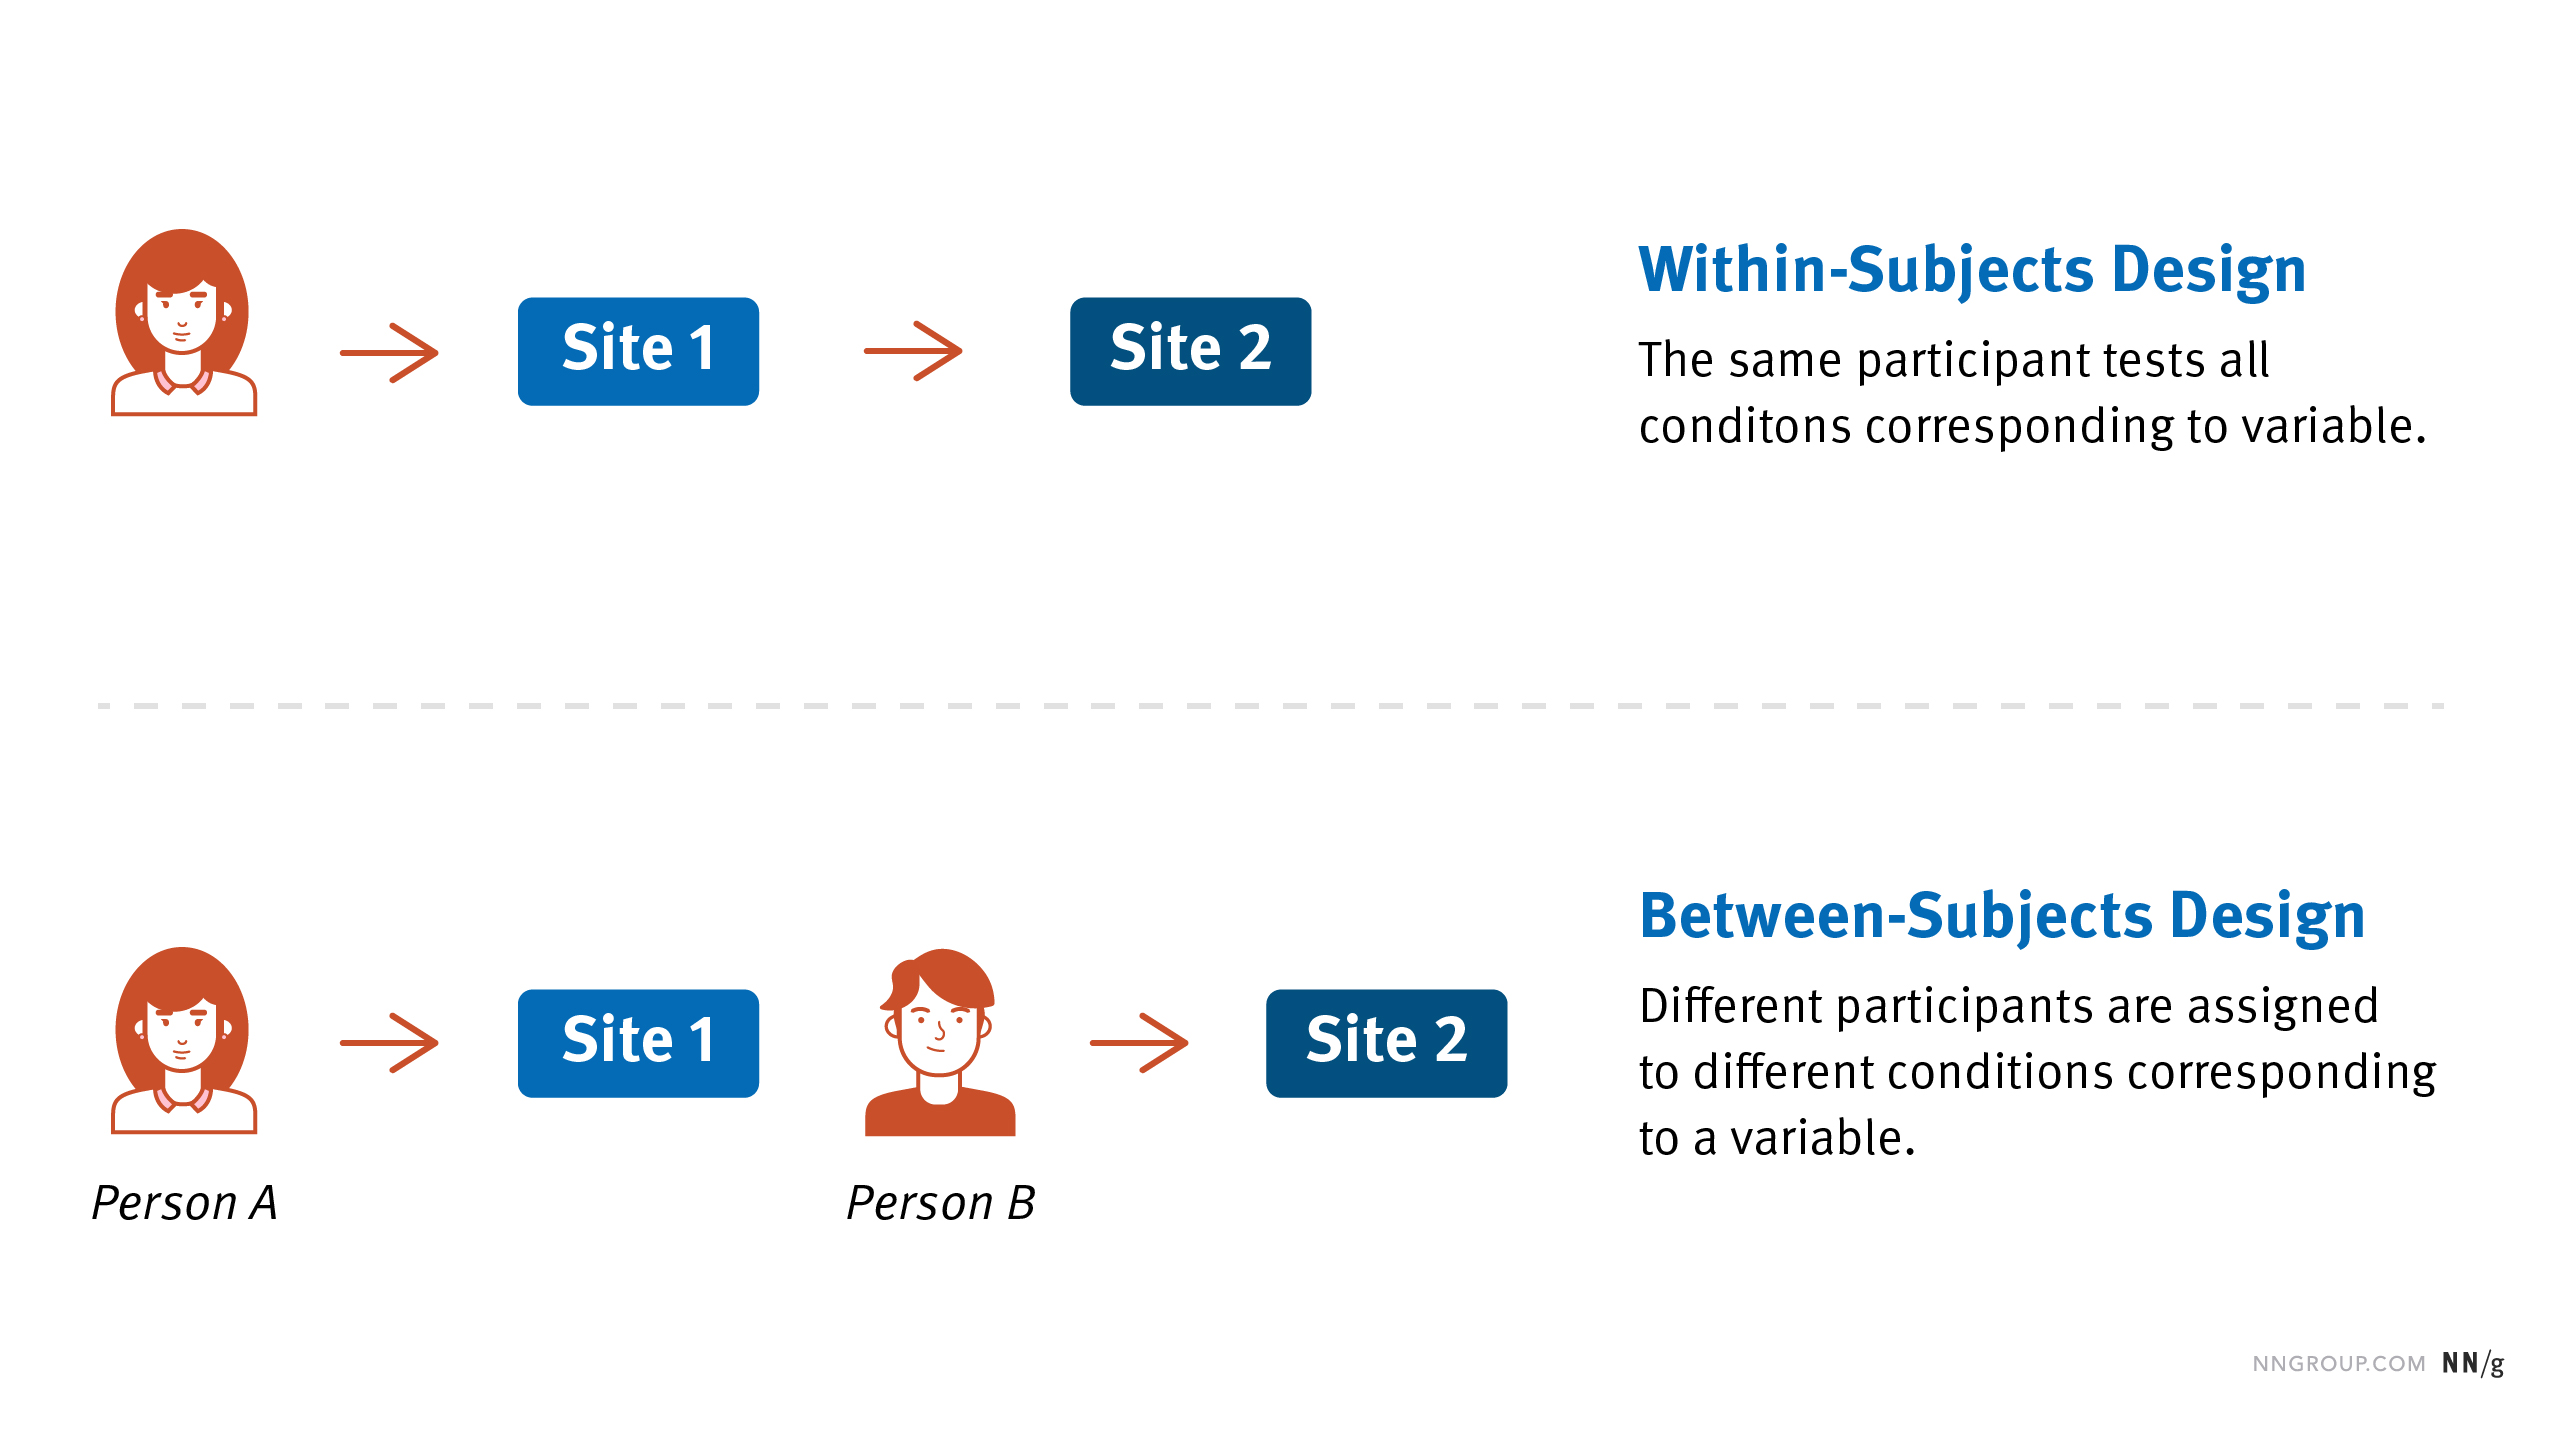
\includegraphics[width=1\linewidth,height=\textheight,keepaspectratio]{images/subject-design-graphic.jpg}}

\textbf{Within-Subjects Design}

In contrast, a \textbf{within-subjects design} involves exposing the same participants to all independent variable levels. This approach allows researchers to observe how changes in the independent variable affect the same individuals, effectively controlling for individual differences. For instance, participants might first watch a news broadcast with a positive tone and later view one with a negative tone, with their reactions measured after each exposure. By comparing responses within the same group, researchers can more precisely determine the impact of the variable.

While within-subjects designs offer the advantage of increased sensitivity to detecting effects, they can also introduce potential issues like order effects. The sequence in which conditions are presented might influence participants' responses due to factors such as fatigue, practice, or carryover effects. To mitigate these concerns, researchers often employ \textbf{counterbalancing} techniques, varying the order of conditions across participants to distribute any order-related influences evenly.

\textbf{Control Groups}

A critical element of any experimental design is including a \textbf{control group}. This group consists of participants who do not receive the experimental treatment and serves as a baseline for comparison. In mass media research, a control group might be exposed to neutral media content, while experimental groups encounter content with specific biases or manipulations. Researchers can determine whether the independent variable has a significant effect by comparing the control group's responses to those of the experimental groups.

Control groups are essential for isolating the impact of the independent variable and ruling out alternative explanations for the findings. Without a control group, it becomes challenging to ascertain whether observed changes are due to the manipulation or other external factors. For example, if both the control and experimental groups exhibit similar changes in perception, this might indicate that factors unrelated to the media content are influencing the results.

\href{https://www.thoughtco.com/control-and-experimental-group-differences-606113}{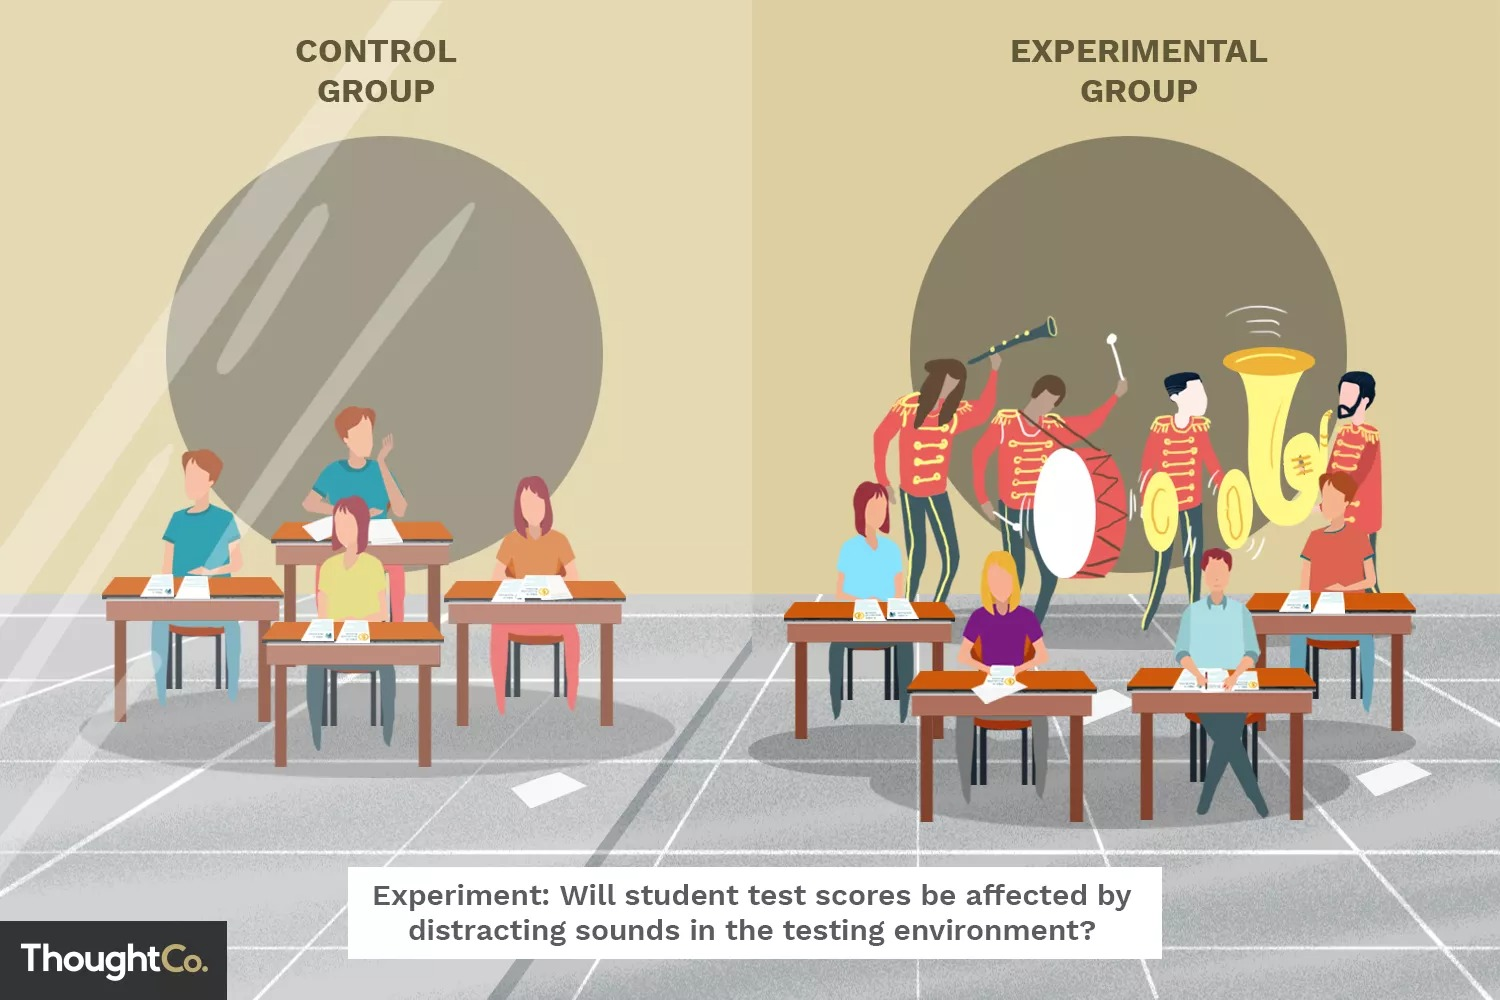
\includegraphics[width=1\linewidth,height=\textheight,keepaspectratio]{images/control.jpg}}

\textbf{Applying Experimental Designs in Mass Media Research}

Understanding how to implement these experimental designs properly is crucial for conducting valid and reliable research in mass media. Through carefully structured experiments, researchers can explore questions such as:

\begin{itemize}
\tightlist
\item
  How does the framing of news stories influence audience attitudes toward social issues?
\item
  What is the effect of exposure to violent media content on aggressive behavior?
\item
  How do different advertising strategies impact consumer purchasing decisions?
\end{itemize}

By selecting the appropriate experimental design, researchers can tailor their studies to effectively address specific research questions. For instance, a between-subjects design might be ideal for comparing the effects of two distinct advertising campaigns on separate groups. Conversely, a within-subjects design could be more suitable for assessing changes in audience perceptions before and after exposure to a particular media message.

\textbf{Conclusion}

Mastering experimental designs empowers researchers to conduct rigorous investigations into the effects of media on audiences. By understanding the strengths and challenges of between-subjects and within-subjects designs, as well as the importance of control groups, researchers can enhance the validity and reliability of their studies. This foundational knowledge is essential for anyone engaged in mass communications research, providing the tools necessary to draw meaningful conclusions about the complex interplay between media content and audience response.

\subsection*{Non-Experimental Designs}\label{non-experimental-designs}
\addcontentsline{toc}{subsection}{Non-Experimental Designs}

In mass media research, not all studies permit experimental manipulation due to ethical, practical, or logistical constraints. In such cases, researchers rely on \textbf{non-experimental designs} to observe and analyze data as it naturally occurs. Two prevalent non-experimental approaches are \textbf{cross-sectional designs} and \textbf{longitudinal designs}. Understanding these methods is essential for conducting meaningful research when experiments are not feasible.

\textbf{Cross-Sectional Designs}

Cross-sectional designs involve observing a specific population at a single point in time. By collecting data simultaneously from different individuals, researchers can identify patterns, trends, and relationships between variables within a population. For example, surveying to assess public opinion on the influence of social media platforms at a particular moment provides a snapshot of current views and behaviors.

The primary advantage of cross-sectional designs is their efficiency. Data collection occurs once, making these studies relatively quick to complete and often less costly than other designs. They are handy for descriptive research aiming to understand the prevalence or distribution of a phenomenon within a population.

However, cross-sectional designs have limitations regarding causal inference. Since data is collected at one point, determining the directionality of relationships between variables or establishing cause-and-effect links is challenging. For instance, if a study finds that individuals who spend more time on social media report higher levels of anxiety, it cannot clarify whether social media use causes anxiety, anxiety leads to increased social media use, or if another factor influences both variables.

\textbf{Longitudinal Designs}

Longitudinal designs involve observing the same participants over an extended period. By tracking changes within the same group of individuals, researchers can more effectively study developments, trends, and potential causal relationships. For example, following a group of participants over several years to examine how prolonged exposure to certain media content influences their political attitudes allows researchers to see how variables evolve and how earlier experiences impact later outcomes.

Longitudinal designs are valuable for studying changes and developments over time. They provide insights into long-term effects and can help establish causality by demonstrating how one variable influences another across different periods. For instance, a longitudinal study might reveal that increased media exposure during adolescence leads to specific changes in political attitudes in adulthood, offering evidence of a causal relationship.

Despite their strengths, longitudinal studies present challenges. Participant attrition, or dropout, is a significant concern. Over time, some participants may leave the study due to loss of interest, relocation, or life changes, which can introduce bias if the remaining participants differ systematically from those who leave. Additionally, longitudinal research is more time-consuming and costly, requiring sustained resources and meticulous planning.

\textbf{Applying Non-Experimental Designs in Mass Media Research}

Understanding the advantages and limitations of cross-sectional and longitudinal designs is crucial for mass media researchers. These designs are often employed when experimental manipulation is not possible, but valuable insights are still needed.

\begin{itemize}
\item
  \textbf{Case Study---Cross-Sectional Design}: A researcher conducts a nationwide survey to explore the relationship between social media usage and trust in traditional news outlets. By analyzing data collected at one point, the researcher identifies correlations and patterns that inform our understanding of media consumption behaviors.
\item
  \textbf{Case Study---Longitudinal Design}: This long-term study follows a group of teenagers over a decade to assess how early exposure to violent video games influences aggressive behavior into adulthood. By collecting data at multiple intervals, the study provides evidence of potential causal links between media exposure and behavioral outcomes.
\end{itemize}

Addressing challenges like participant dropout in longitudinal studies involves maintaining regular contact, offering incentives, and employing tracking methods to keep participants engaged. In cross-sectional studies, careful sampling and statistical controls help mitigate limitations related to causality.

\textbf{Conclusion}

Mastering both cross-sectional and longitudinal designs equips researchers with essential tools for conducting insightful and methodologically sound studies in mass media. While cross-sectional designs offer efficiency and are excellent for identifying current relationships and trends, longitudinal designs provide depth in understanding changes over time and potential causal links. By selecting the appropriate design for specific research questions and being mindful of each approach's strengths and limitations, researchers enhance their findings' validity and impact in the dynamic mass media research field.

\subsection*{Sampling Methods}\label{sampling-methods}
\addcontentsline{toc}{subsection}{Sampling Methods}

The method used to select a sample significantly impacts the validity and generalizability of research findings in mass media studies. \textbf{Sampling methods} determine how participants are chosen from the larger population and are crucial for ensuring that a study accurately represents the intended group. Various sampling methods exist, each with its advantages and limitations. Understanding these methods helps researchers make informed decisions about study design and result interpretation.

\textbf{Random Sampling}

One of the most influential and widely used methods is \textbf{random sampling}. In this approach, participants are selected so that every member of the population has an equal chance of being chosen. Random sampling is considered the gold standard because it minimizes selection bias and enhances the generalizability of study results.

For example, suppose a researcher surveys viewers to understand their preferences for television programs. By randomly selecting viewers from a television network's entire subscriber list, each subscriber---regardless of viewing habits---has an equal chance of inclusion. This randomness helps ensure the sample is representative of the larger population, allowing for more confident generalization of the findings.

Random sampling is particularly valuable when drawing conclusions that apply broadly to the entire population. However, careful planning and sometimes a larger sample size are required to reflect the population's diversity truly. While random sampling reduces bias, it does not eliminate it; factors such as non-response can still introduce some bias.

\begin{figure}
\centering
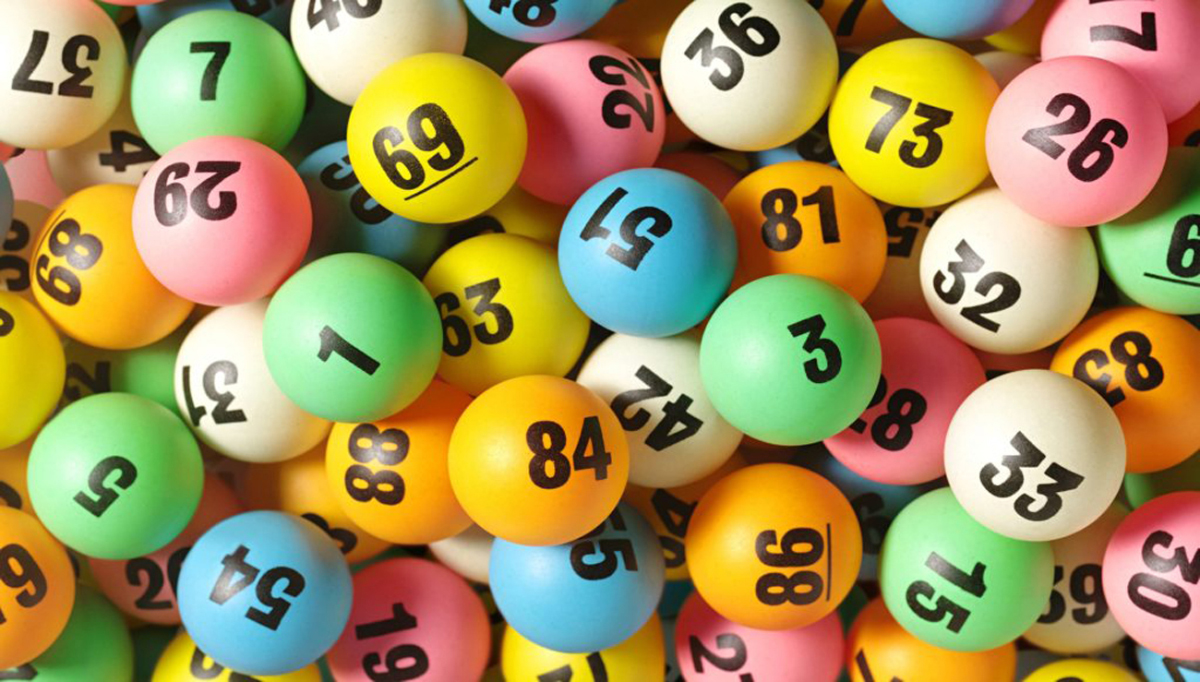
\includegraphics[width=1\linewidth,height=\textheight,keepaspectratio]{images/random.jpg}
\caption{Lottery balls}
\end{figure}

\textbf{Stratified Sampling}

Another critical method is \textbf{stratified sampling}, which involves dividing the population into distinct subgroups or strata and randomly sampling from each group. This approach ensures that each subgroup is adequately represented in the sample, especially when specific characteristics---such as age, gender, or income level---are essential for the research.

For instance, if studying media preferences across different age groups, a researcher might divide the population into age strata (e.g., 18--29, 30--49, 50 and above) and randomly select participants from each group. This method ensures that each age group is proportionally represented, allowing for more precise comparisons between groups.

Stratified sampling is particularly beneficial when the population is heterogeneous, meaning there are significant differences between subgroups. Ensuring proportional representation improves the accuracy of estimates and reduces sampling error. However, it requires detailed knowledge of the population and can be more complex to implement than simple random sampling.

\begin{figure}
\centering
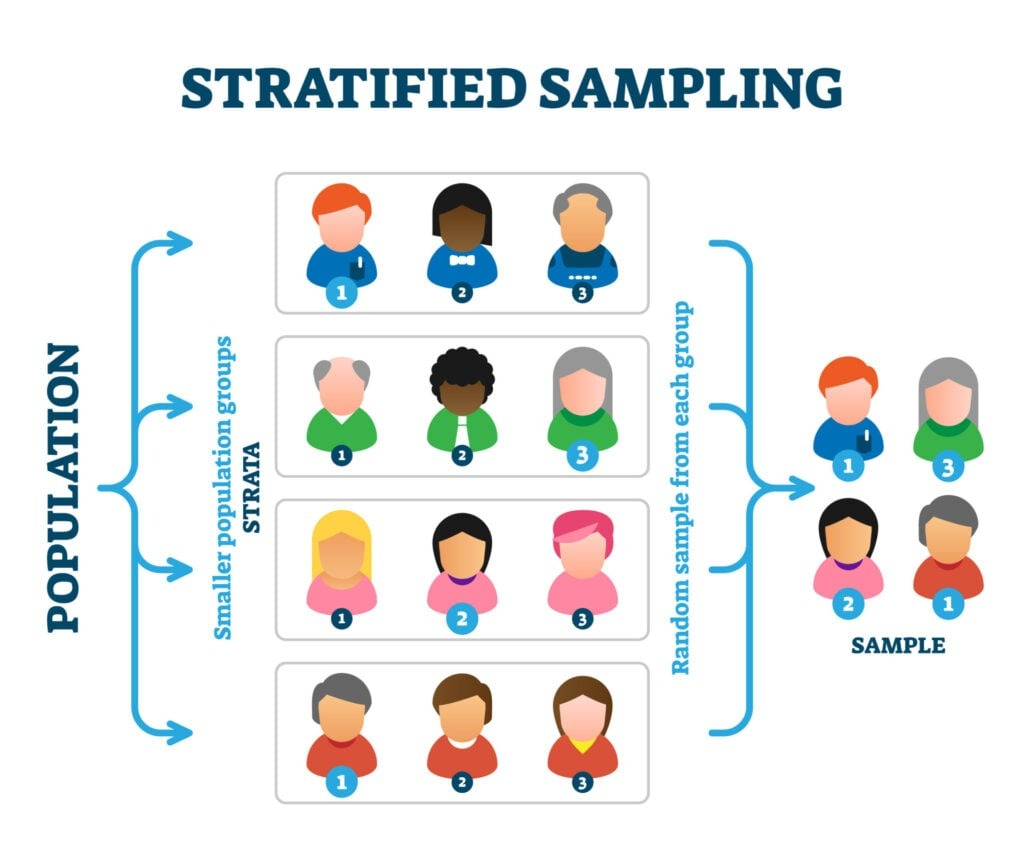
\includegraphics[width=1\linewidth,height=\textheight,keepaspectratio]{images/strata.jpg}
\caption{Representation of stratified sampling}
\end{figure}

\textbf{Convenience Sampling}

In contrast, \textbf{convenience sampling} involves selecting participants who are readily available and accessible to recruit. While practical and cost-effective, this method has significant limitations regarding representativeness and generalizability.

For example, convenience sampling is used to research media habits among college students by surveying students in one's classes. Although straightforward, this sample may not represent all college students or the general population, potentially leading to biases in the findings.

Convenience sampling is often employed in exploratory research, pilot studies, or situations where other methods are not feasible. However, it is crucial to recognize its limitations: since the sample is not randomly selected, results may not be generalizable beyond the specific group studied. To mitigate some drawbacks, researchers can combine convenience sampling with other techniques, such as increasing the sample size or using quota sampling, to ensure some level of diversity within the sample.

\textbf{Applying Sampling Methods in Mass Media Research}

Understanding and correctly applying these sampling methods is vital in mass media research, where accurately capturing audience diversity is essential.

\begin{itemize}
\item
  \textbf{Random Sampling Case Study}: A national survey assessing public trust in news media employs random sampling to include a wide range of demographic groups, enhancing the study's generalizability.
\item
  \textbf{Stratified Sampling Case Study}: A study examining social media usage patterns divides participants into different age groups and samples each subgroup proportionally, ensuring meaningful comparisons across ages.
\item
  \textbf{Convenience Sampling Case Study}: A researcher might survey people at a local shopping mall for a preliminary study on reactions to a new advertising campaign. While offering immediate insights, the findings may not be generalizable to the broader population.
\end{itemize}

\textbf{Conclusion}

By mastering random, stratified, and convenience sampling methods, researchers are better equipped to select the most appropriate approach for their questions and understand each method's implications for their findings. This knowledge is essential for conducting rigorous and credible research in mass media studies, where the sample's representativeness directly affects the results' validity.

\section{Data Collection Techniques}\label{data-collection-techniques}

\subsection*{Surveys and Questionnaires}\label{surveys-and-questionnaires}
\addcontentsline{toc}{subsection}{Surveys and Questionnaires}

Surveys and questionnaires are fundamental tools in mass media research, enabling efficient data collection from many participants. They allow researchers to gather information on attitudes, behaviors, preferences, and other variables of interest. The design of survey questions is critical to ensure that the data collected is accurate, meaningful, and truly reflective of respondents' opinions. Understanding the different types of survey questions---such as Likert-type items, closed-ended and open-ended questions---is essential for designing effective surveys.

\textbf{Likert-Type Items}

One of the most widely used types of survey questions is the \textbf{Likert-type item}. This format presents a statement to which respondents indicate their level of agreement on a scale, typically ranging from ``strongly disagree'' to ``strongly agree.'' For example, a survey might ask respondents to rate their agreement with the statement, ``Social media has a positive impact on society,'' using a scale from 1 (strongly disagree) to 5 (strongly agree). Likert-type items are beneficial for measuring attitudes and opinions because they provide a clear, quantifiable way to capture the strength of respondents' feelings on an issue.

The advantages of Likert-type items include their simplicity and standardization, which facilitate easy comparison across respondents. Because the scale is consistent across items, these questions can be used to create composite scores that reflect overall attitudes toward a topic. However, careful attention must be paid to the wording of the statements to avoid bias. Leading or ambiguous statements can skew responses, resulting in data that does not accurately reflect genuine opinions.

\begin{figure}
\centering
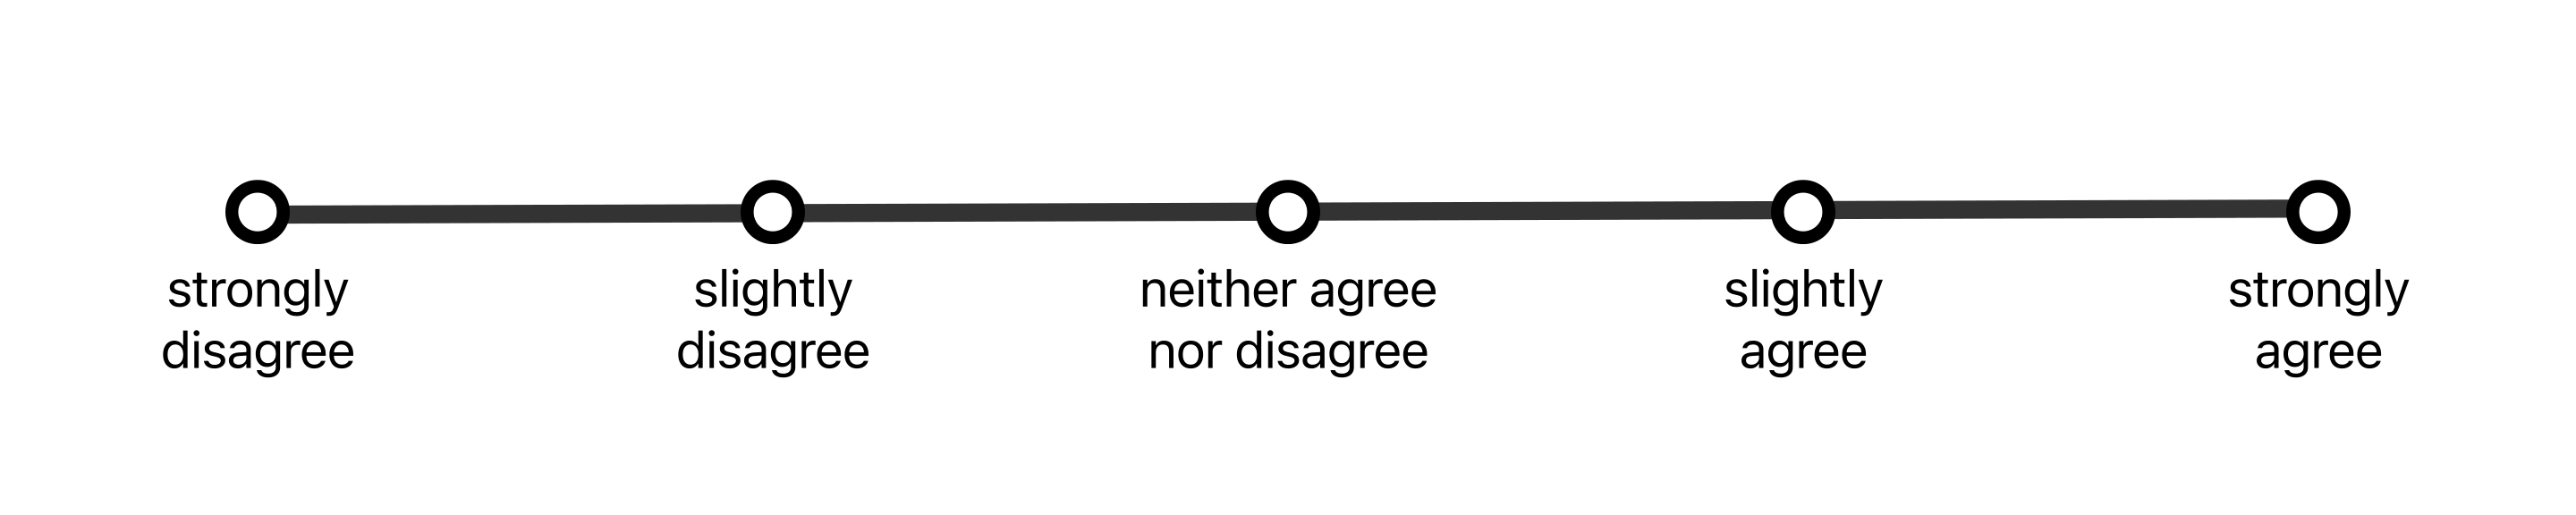
\includegraphics[width=1\linewidth,height=\textheight,keepaspectratio]{images/likert-scale.png}
\caption{Likert-type scale}
\end{figure}

\textbf{Closed-Ended Questions}

\textbf{Closed-ended questions} provide respondents with a set of predefined responses to choose from. For example, a survey might ask, ``How often do you use social media?'' with response options like ``Daily,'' ``Weekly,'' ``Monthly,'' or ``Never.'' Closed-ended questions are highly efficient for collecting data because they are easy to answer and straightforward to analyze. They allow for quick comparisons and statistical analysis across different respondents.

The main advantage of closed-ended questions is their simplicity and ease of analysis. Since the responses are predefined, researchers can quickly categorize and quantify the data, making it easier to identify patterns and trends. However, a limitation is that they may constrain respondents' answers, potentially losing nuanced information. If the predefined options do not fully capture respondents' actual behaviors or opinions, the data collected may be inaccurate.

\textbf{Open-Ended Questions}

In contrast, \textbf{open-ended questions} allow respondents to answer in their own words, providing richer and more detailed data. For example, a survey might ask, ``What do you think is the most significant impact of social media on society?'' This type of question allows respondents to express their thoughts and opinions without being confined to predefined responses.

Open-ended questions are valuable because they can uncover insights that might be missed with closed-ended questions. They enable respondents to provide more nuanced and personal responses, revealing underlying attitudes, motivations, or concerns. However, the trade-off is that open-ended questions can be more challenging to analyze. The varied and complex nature of the responses requires careful coding and interpretation, which can be time-consuming.

\textbf{Design Considerations}

When designing surveys and questionnaires, it is crucial to consider the appropriate context for each type of question. Likert-type items are effective for measuring attitudes and opinions on a scale, closed-ended questions help collect quantifiable data efficiently, and open-ended questions are ideal for exploring complex issues in depth. Attention to question-wording, response options, and potential biases is essential to ensure that the data collected is accurate and meaningful.

\textbf{Conclusion}

By mastering Likert-type items and closed-ended and open-ended questions, researchers will be well-equipped to design surveys and questionnaires that effectively gather the necessary information. Understanding the appropriate context for each type of question and the implications for data analysis is essential for conducting rigorous and insightful research in mass communications.

\subsection*{Observation Methods}\label{observation-methods}
\addcontentsline{toc}{subsection}{Observation Methods}

Observation methods are essential in mass media research, allowing researchers to study behaviors, interactions, and environments in their natural settings. Unlike surveys or experiments, which often involve some degree of control or intervention, observation methods enable data collection in an organic and unstructured way. Various observation techniques exist, each offering unique insights into human behavior. Understanding methods such as participant observation, complete observation, and direct observation enhances the ability to design and conduct research that captures the complexity of media interactions.

\textbf{Participant Observation}

In \textbf{participant observation}, the researcher actively engages in the environment or group being studied while simultaneously observing behaviors. This method is beneficial for studying social interactions and cultural practices, providing an insider's perspective. For example, a researcher might join an online forum that discusses news events to observe how users interact and share information. By becoming a participant, the researcher experiences the group's dynamics firsthand, gaining insights that might not be accessible through detached observation.

However, participant observation presents challenges, especially regarding ethical considerations and potential observer bias. The researcher's presence and actions can influence the behavior of those being observed, a phenomenon known as the observer effect. Additionally, the researcher's beliefs and experiences may color their observations, leading to bias in data collection. Maintaining a balance between engagement and objectivity is crucial, as is knowing how participation might affect the data.

\begin{figure}
\centering
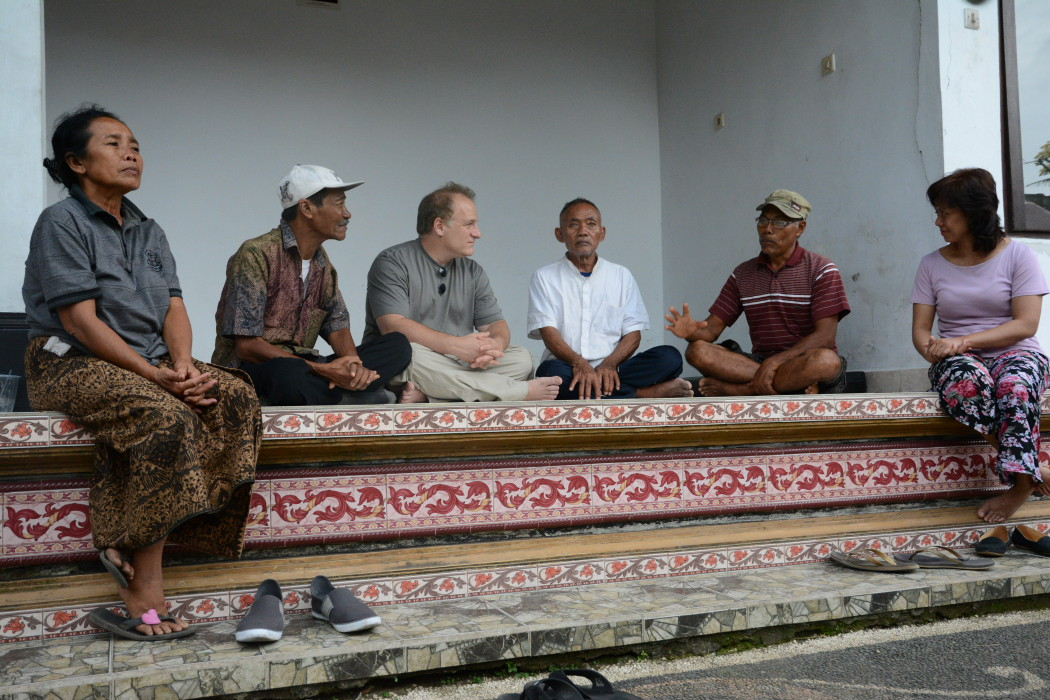
\includegraphics[width=1\linewidth,height=\textheight,keepaspectratio]{images/part-observation.jpg}
\caption{Participant observation in ethnography}
\end{figure}

\textbf{Complete Observation}

The \textbf{complete observer} method involves the researcher observing the environment without interacting or participating. This approach minimizes the researcher's influence on the subjects, as participants are often unaware they are being observed. For instance, a researcher might observe interactions in a public place, such as a park or café, without engaging with the people being studied. By maintaining distance, the researcher can capture behaviors as they naturally occur, reducing the risk of altering the environment's dynamics.

While the complete observer role reduces the observer effect, it also has limitations. One main drawback is the potential lack of depth in the data collected. Without engaging with participants, the researcher may miss the context or motivations behind certain behaviors. Ethical concerns can also arise, particularly regarding privacy and informed consent, especially in settings where participants are unaware of the observation.

\textbf{Direct Observation}

\textbf{Direct observation} involves systematically watching and recording behaviors or events as they naturally occur. Unlike participant observation, where the researcher engages with the environment, or complete observation, where the researcher remains detached, direct observation focuses on the structured recording of specific behaviors. For example, a researcher might observe and record the frequency of certain media consumption behaviors in a public space, such as how often people check their phones in a café.

Direct observation is helpful for studies requiring precise and quantifiable data on specific behaviors. It allows researchers to collect directly observable data, reducing reliance on self-reported information, which can be inaccurate or biased. However, maintaining consistency in recording behaviors and ensuring the observation process does not become intrusive are challenges that must be addressed.

\textbf{Applying Observation Methods in Mass Media Research}

Mastering these observation methods equips researchers to choose the most appropriate approach for their questions and conduct studies that capture the complexity of human behavior in media contexts. Each method offers unique insights and challenges:

\begin{itemize}
\item
  \textbf{Participant Observation Case Study}: A researcher can gain insider perspectives on how information is shared and opinions are formed by joining an online community discussing current events.
\item
  \textbf{Complete Observation Case Study}: Observing interactions in a public setting without participation can reveal patterns in media consumption behaviors, such as how people engage with public digital displays.
\item
  \textbf{Direct Observation Case Study}: Systematically recording the frequency of smartphone use during social gatherings can provide quantifiable data on media habits.
\end{itemize}

Understanding when and how to use each method enhances the ability to gather meaningful and reliable data. Ethical considerations, such as informed consent and privacy, are paramount in observational research and must be carefully managed.

\textbf{Conclusion}

Observation methods are invaluable in mass media research for capturing the nuances of human behavior and media interactions. By effectively employing participant observation, complete observation, and direct observation, researchers can collect rich data that surveys or experiments might miss. This depth of understanding is essential for analyzing the complex ways in which media influences society and individual behaviors.

\subsection*{Content Analysis}\label{content-analysis}
\addcontentsline{toc}{subsection}{Content Analysis}

Content analysis is a systematic research method used to interpret and quantify media content by categorizing communication elements and examining the presence, meanings, and relationships of specific words, themes, or concepts. In mass media research, content analysis is invaluable for studying patterns, trends, and the influence of media messages on audiences. It enables researchers to uncover explicit and implicit messages conveyed through various media forms.

\textbf{Manifest Content Analysis}

\textbf{Manifest content} refers to the explicit, surface-level elements of media content that are directly observable and quantifiable. This includes the frequency of specific words, phrases, images, or other tangible components within a text or media piece. For example, a researcher might conduct a manifest content analysis to count how often the term ``climate change'' appears in newspaper articles over a certain period. By quantifying these occurrences, researchers can identify trends in topic coverage or the prominence of specific terms in the media.

The advantages of manifest content analysis lie in its objectivity and replicability. Since it focuses on observable data, the results are less subject to researcher bias and can be easily compared across different studies. However, while manifest content analysis effectively tells us what is present in the media, it does not delve into the deeper meanings or implications behind the content. For instance, knowing that ``climate change'' is frequently mentioned does not reveal whether the coverage is positive, negative, or neutral or what underlying messages are being conveyed.

Researchers often examine various media forms, such as newspapers, television broadcasts, and social media posts, to illustrate the application of manifest content analysis. By coding manifest content---such as counting keywords or categorizing images---they can systematically analyze media content. Clear coding guidelines are essential to ensure consistency and accuracy across the analysis.

\textbf{Latent Content Analysis}

In contrast, \textbf{latent content} refers to the underlying meanings, themes, or messages embedded within media content that are not immediately apparent. Latent content analysis goes beyond the surface to explore deeper significance, such as tone, bias, or ideological perspectives. For example, when analyzing a news article on political events, a researcher might examine whether the coverage subtly favors one political party over another or presents events positively or negatively.

Identifying and interpreting latent content is more complex and involves subjective judgment and interpretation. Different researchers might interpret the same content differently, leading to variability in findings. Therefore, latent content analysis often requires a nuanced approach and a thorough understanding of the context in which the content was produced and consumed.

The complexities of latent content analysis can be explored through case studies, where researchers analyze media samples to uncover hidden themes or biases. Engaging in group analyses to identify latent themes can highlight the subjectivity involved and the critical thinking required to conduct such analysis effectively.

\textbf{The Coding Process}

The process of coding is central to both manifest and latent content analysis. Coding involves categorizing and tagging content to identify patterns, themes, or trends within qualitative data. It allows researchers to systematically organize and interpret large amounts of data, making it easier to draw meaningful conclusions.

Developing a coding scheme is a critical step in content analysis. A well-defined coding scheme should be clear, consistent, and applicable across texts or media samples. For instance, researchers might develop codes to categorize media content as ``informative,'' ``persuasive,'' or ``entertainment.'' Applying this coding scheme to a sample of media texts enables analysis of the prevalence and distribution of these content types across platforms or periods.

Achieving \textbf{inter-coder reliability} is essential to ensure the validity of findings. This means that multiple researchers independently coding the same content should reach similar conclusions. Consistency in coding reduces bias and increases the credibility of the analysis.

\begin{figure}
\centering
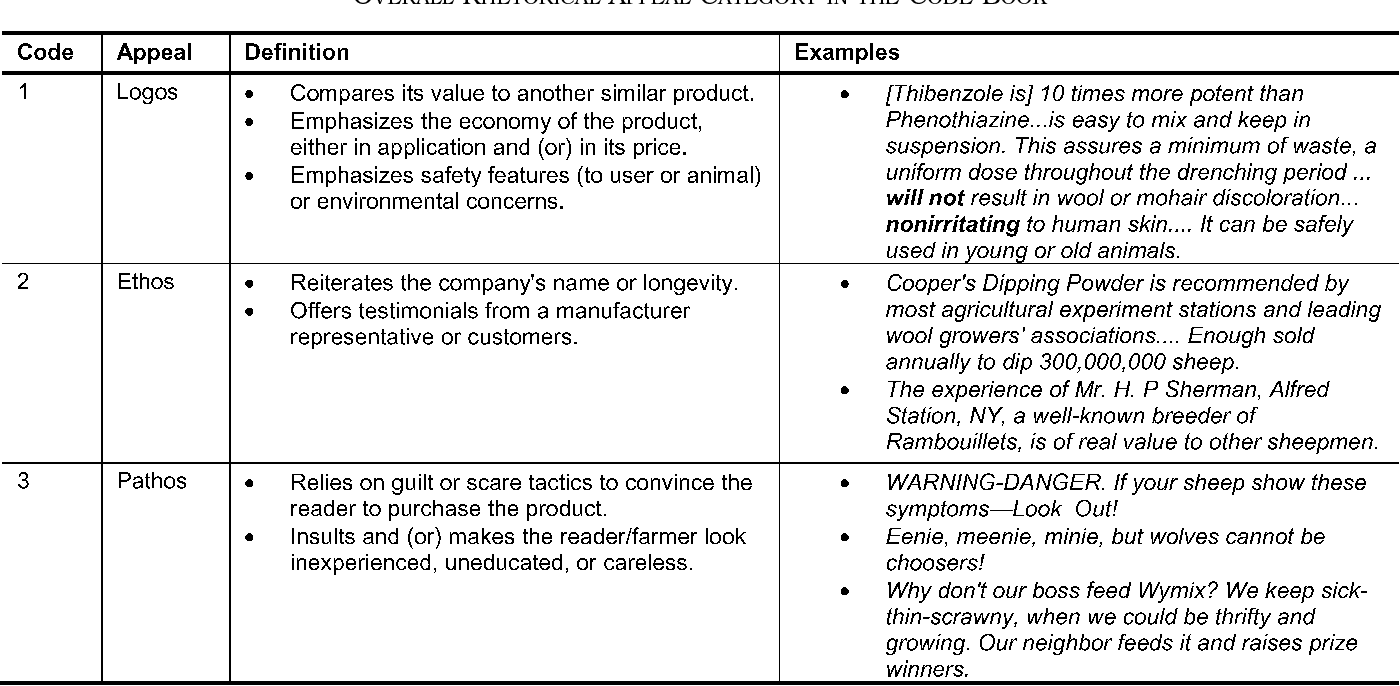
\includegraphics[width=1\linewidth,height=\textheight,keepaspectratio]{images/quant-content-scheme.png}
\caption{Coding scheme for a quantitative content analysis.}
\end{figure}

\textbf{Applying Content Analysis in Mass Media Research}

By mastering manifest and latent content analysis techniques, researchers can conduct rigorous and insightful examinations of media content. These skills allow for uncovering both visible and hidden messages within the media, contributing to a deeper understanding of how media shapes and reflects societal values, beliefs, and behaviors.

For example, content analysis can be used to study:

\begin{itemize}
\tightlist
\item
  \textbf{Gender Representation}: Examining how different genders are portrayed in advertising to identify stereotypes or biases.
\item
  \textbf{Political Framing}: Analyzing news coverage to see how political issues are presented and which narratives are promoted.
\item
  \textbf{Cultural Trends}: Tracking the prevalence of specific themes or topics in social media to understand shifting public interests.
\item
  \textbf{Media Influence}: Investigating how frequently particular health messages appear in media and their potential impact on public behavior.
\end{itemize}

By systematically analyzing media content, researchers can identify patterns and trends that inform our understanding of the media's role in society.

\textbf{Conclusion}

Content analysis is a powerful method in mass media research for systematically examining media content. Whether focusing on explicit elements through manifest content analysis or exploring deeper meanings through latent content analysis, this method enables researchers to decode the complex messages conveyed by the media. The coding process is central to organizing and interpreting data effectively, and developing a reliable coding scheme is crucial for producing valid and meaningful results.

Understanding and applying content analysis equips researchers with the tools to critically assess media content, providing valuable insights into how media influences and reflects the world. These skills are essential for conducting thorough and impactful research in mass communications.

\chapter{Selecting and Adapting Research Scales}\label{selecting-and-adapting-research-scales}

This chapter aims to provide a comprehensive understanding of the use and adaptation of research scales in mass communications. It will guide students through the process of selecting reliable and valid scales, adapting them to specific research needs, and doing so with ethical and legal considerations in mind. This will ensure that students are equipped to effectively measure complex constructs in mass communication research.

\section*{Overview of Research Scales in Mass Communications}\label{overview-of-research-scales-in-mass-communications}
\addcontentsline{toc}{section}{Overview of Research Scales in Mass Communications}

\subsection*{Introduction to Widely Used Scale Types}\label{introduction-to-widely-used-scale-types}
\addcontentsline{toc}{subsection}{Introduction to Widely Used Scale Types}

\subsubsection*{Likert Scales}\label{likert-scales}
\addcontentsline{toc}{subsubsection}{Likert Scales}

The Likert scale is extensively used for gauging attitudes and opinions in social media research. It typically presents respondents with a statement and asks them to express their level of agreement or disagreement on a five or seven-point scale, ranging from ``strongly disagree'' to ``strongly agree.'' This format is particularly useful for measuring public opinion on various media topics, including reactions to social media posts, user sentiments about trending topics, or attitudes towards digital campaigns. The Likert scale's simplicity and versatility make it a fundamental tool in social media analytics, enabling researchers to quantify subjective data like opinions and attitudes.

\begin{figure}
\centering
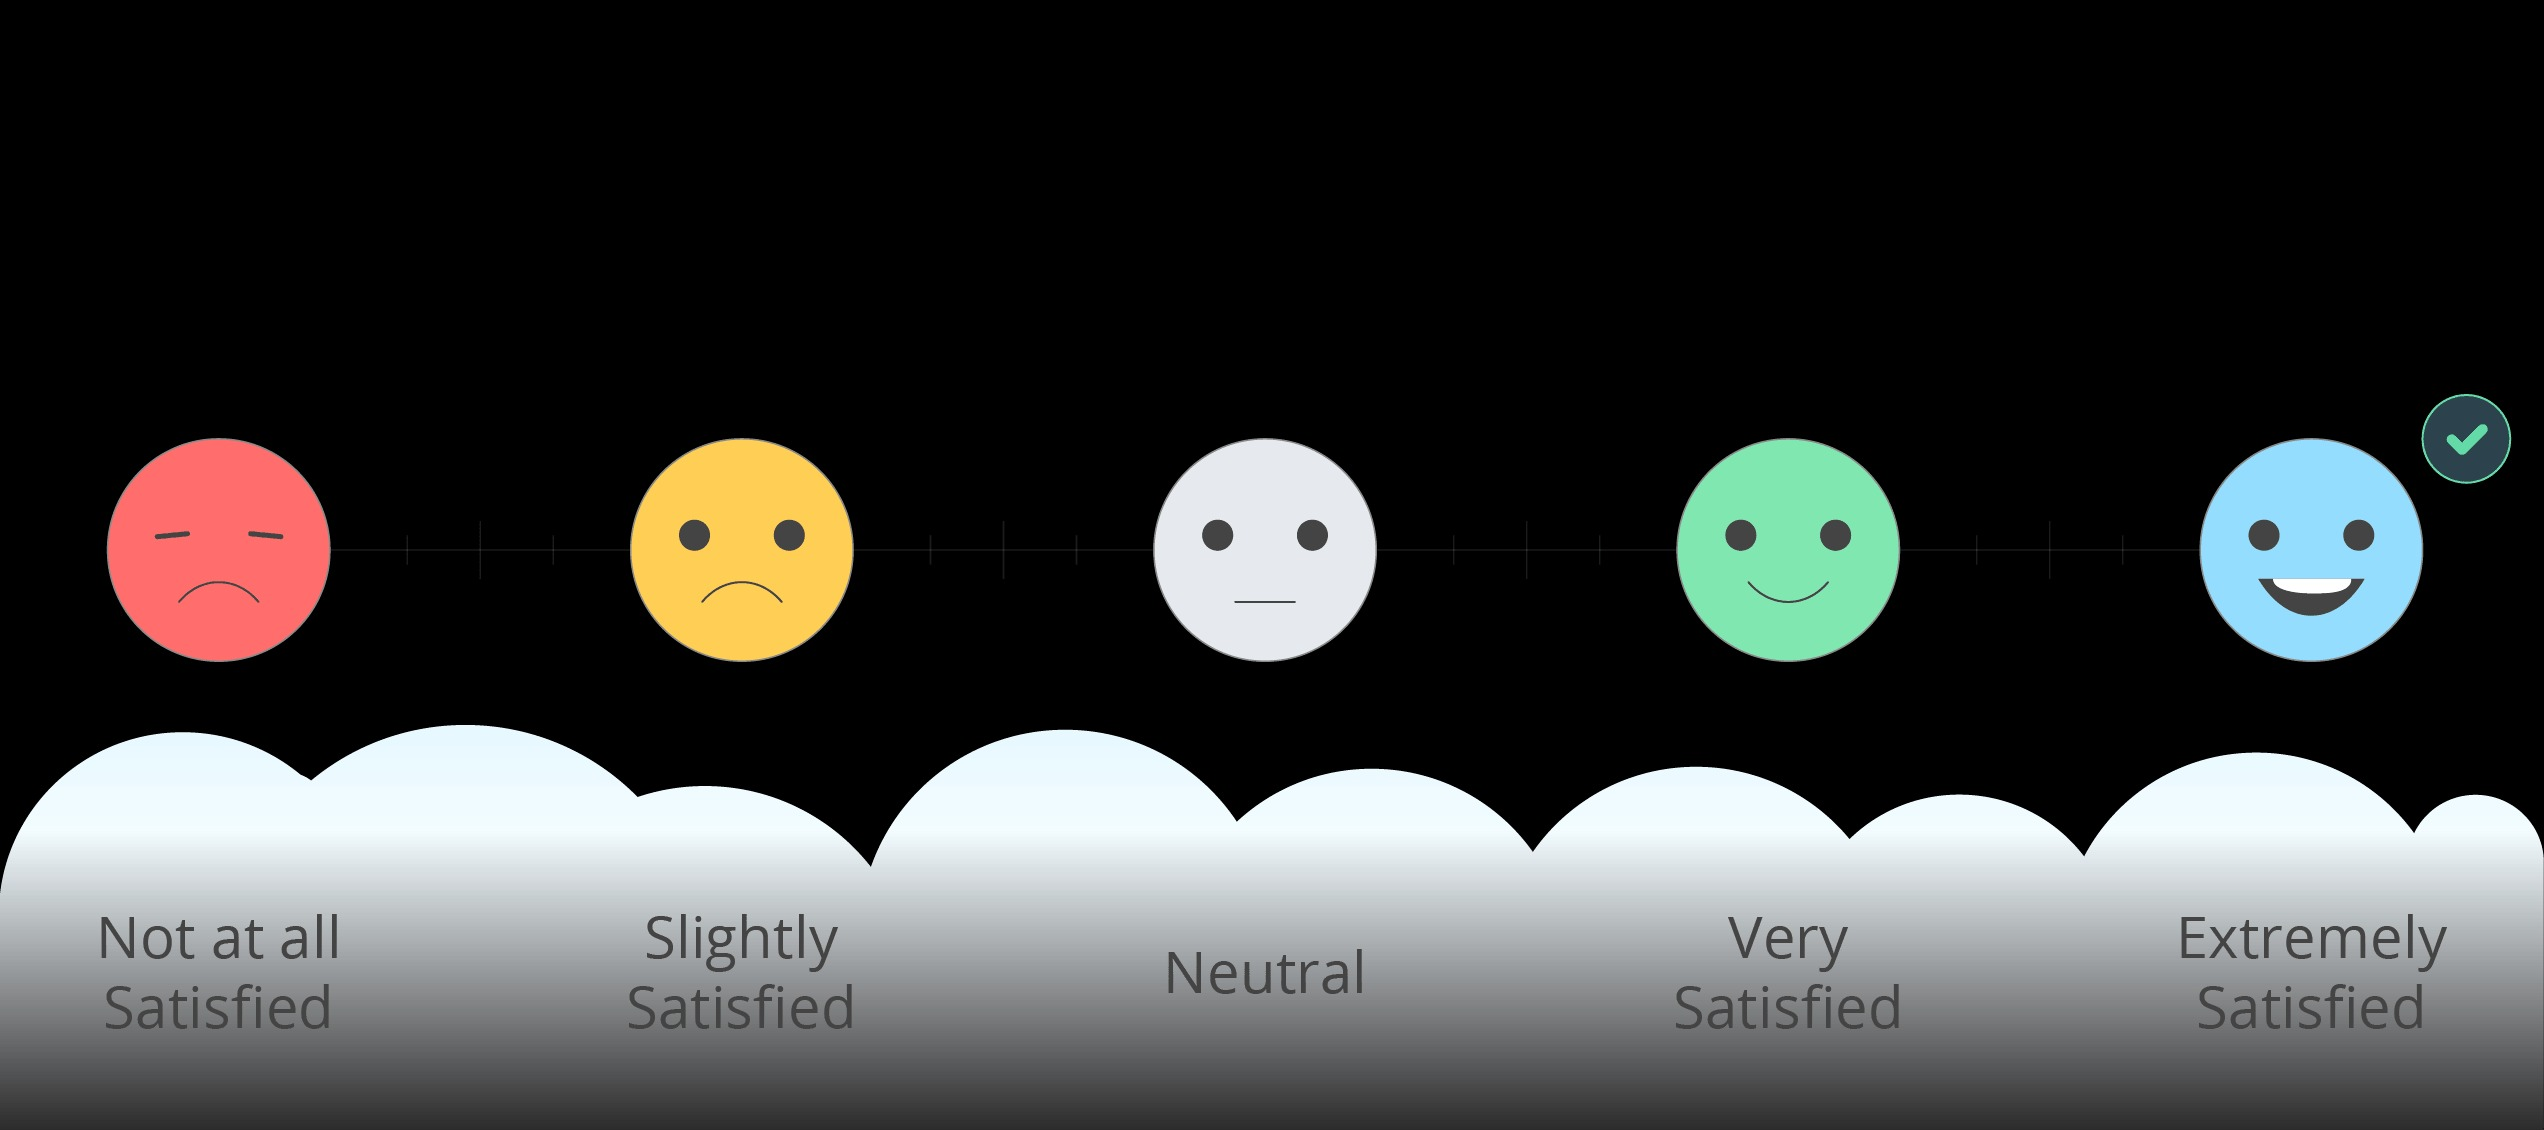
\includegraphics[width=1\linewidth,height=\textheight,keepaspectratio]{images/likert.jpg}
\caption{Facebook Intensity Measure (Ellison, Steinfield, \& Lampe, 2007)}
\end{figure}

\subsubsection*{Semantic Differential Scales}\label{semantic-differential-scales}
\addcontentsline{toc}{subsubsection}{Semantic Differential Scales}

Semantic differential scales are utilized to assess the connotations associated with media messages, which is particularly relevant in the analysis of social media content. This scale asks respondents to rate a media message using a series of bipolar adjectives, such as ``good-bad,'' ``positive-negative,'' or ``useful-useless.'' In social media research, this scale can be employed to understand how users perceive the tone, sentiment, or general disposition of posts and messages. For instance, it can be used to evaluate public perception of a brand's social media presence or to analyze the emotional tone of user-generated content.

\begin{figure}
\centering
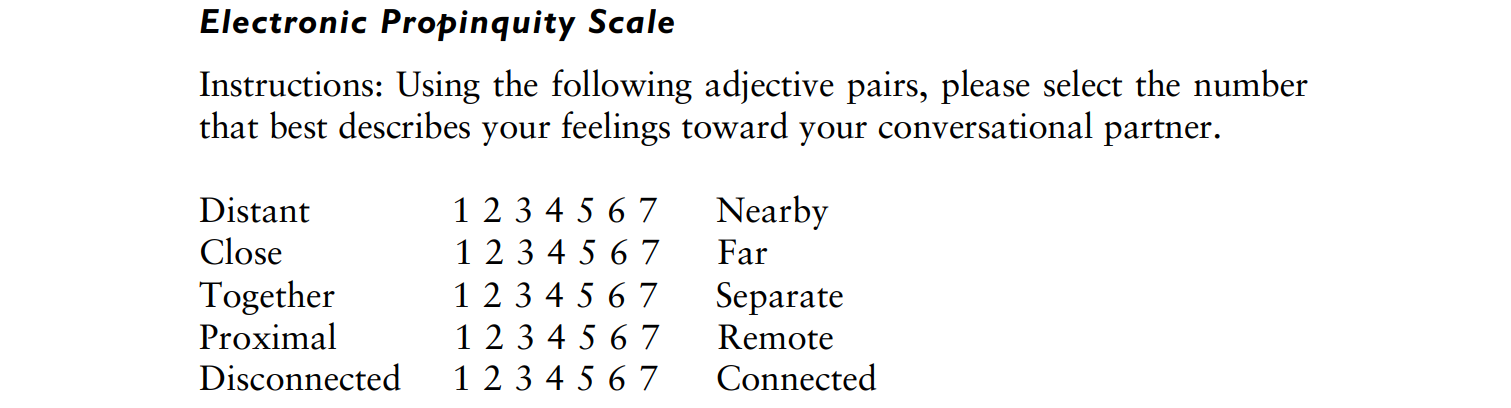
\includegraphics[width=1\linewidth,height=\textheight,keepaspectratio]{images/propinquity.png}
\caption{Electronic Propinquity Scale (Walther \& Bazarova, 2008)}
\end{figure}

\subsubsection*{Engagement Scales}\label{engagement-scales}
\addcontentsline{toc}{subsubsection}{Engagement Scales}

Engagement scales are crucial in social media analytics for measuring how audiences interact with various platforms. These scales are designed to assess different dimensions of media usage and engagement, including the frequency and duration of use, the intensity of engagement, and the emotional connection users have with the content. In a social media context, such scales can help quantify user engagement with specific posts, profiles, or campaigns. They can provide insights into the effectiveness of social media strategies, user involvement levels, and the impact of social media content on audience behavior.

\begin{figure}
\centering

\includegraphics[width=1\linewidth,height=\textheight,keepaspectratio]{images/engagement.jpg}
\caption{Student Engagement Scale (Mazer, 2012)}
\end{figure}

Each of these scales offers unique advantages for social media research. The Likert scale's straightforward format is excellent for survey-based social media research, while the semantic differential scale provides nuanced insights into user perceptions. Engagement scales, on the other hand, are vital for understanding user interaction patterns on social media platforms. The selection and adaptation of these scales depend on the specific research objectives, the nature of the social media content being analyzed, and the characteristics of the target audience.

\subsection*{Specialized Scales in Mass Communications}\label{specialized-scales-in-mass-communications}
\addcontentsline{toc}{subsection}{Specialized Scales in Mass Communications}

\subsubsection*{Audience Satisfaction Scale}\label{audience-satisfaction-scale}
\addcontentsline{toc}{subsubsection}{Audience Satisfaction Scale}

The Audience Satisfaction Scale is designed to assess how viewers or readers feel about the media content they consume. This scale is especially significant in social media analytics, where understanding audience preferences and behavior is key to creating engaging content. By measuring satisfaction, researchers and content creators can gauge the success of their posts, videos, or articles in meeting audience expectations. This scale can involve various metrics, including content enjoyment, fulfillment of informational needs, and overall satisfaction with the media experience.

\subsubsection*{Media Credibility Scale}\label{media-credibility-scale}
\addcontentsline{toc}{subsubsection}{Media Credibility Scale}

In an era where information is abundant and varied, the Media Credibility Scale plays a crucial role in determining which media outlets and content sources are perceived as trustworthy by the audience. This scale evaluates aspects like the perceived accuracy, bias, and reliability of different media sources. In social media analytics, this scale can be applied to measure how audiences perceive the credibility of news shared on social platforms, influencer endorsements, or branded content. Understanding these perceptions is vital for media outlets, marketers, and content creators aiming to build and maintain trust with their audience.

\subsubsection*{Advertising Effectiveness Scale}\label{advertising-effectiveness-scale}
\addcontentsline{toc}{subsubsection}{Advertising Effectiveness Scale}

This scale is essential for evaluating the impact of advertising campaigns on social media. It measures how advertising influences audience perceptions, attitudes, and behaviors. Key components of this scale may include audience recall of the advertisement, changes in attitudes towards the product or brand, and subsequent consumer actions, such as making a purchase or following the brand on social media. The Advertising Effectiveness Scale helps advertisers and marketers to quantify the return on investment of their campaigns and to refine their strategies for greater impact in future campaigns.

Each of these scales offers unique insights into different facets of mass communication in the digital age. By applying these scales in social media analytics, researchers and practitioners can gain a deeper understanding of audience dynamics, media credibility, and the effectiveness of advertising strategies, all of which are crucial in the rapidly evolving landscape of digital media.

\section*{Criteria for Selecting Appropriate Scales}\label{criteria-for-selecting-appropriate-scales}
\addcontentsline{toc}{section}{Criteria for Selecting Appropriate Scales}

\subsection*{Reliability and Validity Considerations}\label{reliability-and-validity-considerations}
\addcontentsline{toc}{subsection}{Reliability and Validity Considerations}

\subsubsection*{Defining Reliability and Validity}\label{defining-reliability-and-validity}
\addcontentsline{toc}{subsubsection}{Defining Reliability and Validity}

\textbf{Reliability}: This term refers to the consistency of a scale over time and across various contexts or samples. A reliable scale is one that yields similar results under consistent conditions. For instance, if a scale measuring audience engagement with a TV show provides consistent results across different audience groups and over multiple episodes, it is considered reliable.

\textbf{Validity}: Validity, conversely, pertains to the accuracy of the scale in measuring what it is intended to measure. This means the scale accurately assesses the specific concept or construct it's supposed to evaluate. For instance, a valid scale for measuring social media influence should accurately assess influence, not just popularity.

\subsubsection*{Illustrating Concepts with Sourcebook Examples}\label{illustrating-concepts-with-sourcebook-examples}
\addcontentsline{toc}{subsubsection}{Illustrating Concepts with Sourcebook Examples}

\textbf{Reliability Example}: To illustrate reliability, consider a scale from the ``Communication Research Measures'' sourcebooks that measures media engagement. For it to be deemed reliable, the scale should consistently measure the level of engagement (such as time spent viewing, likes, and shares) across different studies, showing little variation in results under similar conditions.

\textbf{Validity Example}: As an example of validity, consider a scale designed to assess the credibility of news sources. This scale's validity would be evidenced by its ability to accurately measure the perceived trustworthiness and accuracy of the news, not influenced by unrelated factors like the popularity of the news source or the medium through which the news is delivered.

In summary, the concepts of reliability and validity are crucial in the selection and adaptation of research scales in mass communications and media. Ensuring that a scale is both reliable and valid is key to producing meaningful and trustworthy results in any research study.

\subsection*{Evaluating Scales for Research}\label{evaluating-scales-for-research}
\addcontentsline{toc}{subsection}{Evaluating Scales for Research}

\subsubsection*{Assessing Reliability}\label{assessing-reliability}
\addcontentsline{toc}{subsubsection}{Assessing Reliability}

\textbf{Test-Retest Reliability}: This method involves administering the same scale to the same group of people at two different points in time. A high correlation between the two sets of results indicates good test-retest reliability.

\textbf{Inter-Rater Reliability}: This assessment is crucial when the scale involves subjective judgments. It measures the extent to which different raters or observers give consistent estimates.

\textbf{Internal Consistency}: Often measured using Cronbach's alpha, this method assesses whether the items on a scale are all measuring the same underlying attribute. A high Cronbach's alpha value (typically above 0.7) suggests good internal consistency.

\subsubsection*{Determining Validity}\label{determining-validity}
\addcontentsline{toc}{subsubsection}{Determining Validity}

\textbf{Content Validity}: This aspect checks whether the scale fully represents the concept it is intended to measure. It involves expert evaluation to ensure the scale covers the breadth of the concept.

\textbf{Criterion-Related Validity}: This form of validity is assessed by comparing the scale with another measure that is already accepted as valid. A high correlation with this criterion indicates good criterion-related validity.

\textbf{Construct Validity}: It involves evaluating whether the scale truly measures the theoretical construct it intends to measure. This is often achieved through factor analysis or correlating the scale with other variables that are theoretically related to the construct.

\subsubsection*{Practical Examples from Sourcebooks}\label{practical-examples-from-sourcebooks}
\addcontentsline{toc}{subsubsection}{Practical Examples from Sourcebooks}

The ``Communication Research Measures'' sourcebooks provide real-world examples of how various scales have been evaluated for reliability and validity. By carefully evaluating the reliability and validity of research scales, researchers in mass communications and media can ensure that their studies are built on solid, scientifically sound foundations. This process is crucial for the credibility and generalizability of their research findings.

\begin{enumerate}
\def\labelenumi{\arabic{enumi}.}
\tightlist
\item
  \textbf{Argumentativeness Scale}: Developed by Infante and Rancer (1982), this scale measures individuals' tendencies to approach or avoid arguments. A study by Infante, Myers, and Buerkel (1994) titled ``Argument and Verbal Aggression in Constructive and Destructive Family and Organizational Disagreements'' utilized this scale to examine the relationship between argumentativeness and verbal aggression in different contexts.
\item
  \textbf{Communication Satisfaction Questionnaire (CSQ)}: Developed by Downs and Hazen (1977), the CSQ measures satisfaction with various aspects of organizational communication. A study by Hecht (1978) titled ``The Measurement of Communication Satisfaction'' used the CSQ to assess communication satisfaction within an organization and its relationship with job satisfaction.
\item
  \textbf{Interpersonal Communication Competence Scale}: Developed by Rubin, Martin, and Bruning (1993), this scale assesses one's perceived effectiveness in interpersonal communication. A study by Rubin, Martin, Bruning, and Powers (1993) titled ``Test of a Model of Interpersonal Communication Competence'' used this scale to analyze the factors contributing to effective interpersonal communication.
\item
  \textbf{Organizational Communication Scale}: This scale focuses on communication patterns within organizations. A study by Goldhaber and Rogers (1979), ``Audience Analysis for Communication Audit Research: A Question of Strategy,'' used a version of this scale to evaluate communication strategies within organizations.
\item
  \textbf{Source Credibility Scale}: Developed by McCroskey and Teven (1999), this scale measures perceived credibility of communication sources. A study by McCroskey, Richmond, and McCroskey (2006) titled ``An Examination of the Relationship Between Teacher Credibility and Student Learning'' used this scale to assess the impact of teacher credibility on student learning.
\item
  \textbf{Unwillingness-to-Communicate Scale}: Developed by Burgoon (1976), this scale measures individuals' general reluctance to communicate. A study by McCroskey and Richmond (1987), ``Willingness to Communicate and Interpersonal Communication,'' used this scale to explore the relationship between unwillingness to communicate and various aspects of interpersonal communication.
\end{enumerate}

These studies exemplify the application of each scale in real-world research, demonstrating their utility in diverse areas of communication studies. Each of these scales has been instrumental in advancing our understanding of communication processes in different contexts.

\textbf{\emph{References (in citation order)}}

\begin{itemize}
\tightlist
\item
  Infante, D. A., \& Rancer, A. S. (1982). A conceptualization and measure of argumentativeness. \emph{Journal of Personality Assessment, 46}(1), 72-80. \url{https://doi.org/10.1207/s15327752jpa4601_13}
\item
  Infante, D. A., Myers, S. A., \& Buerkel, R. A. (1994). Argument and verbal aggression in constructive and destructive family and organizational disagreements. \emph{Western Journal of Communication, 58}(2), 73-84. \url{https://doi.org/10.1080/10570319409374466}
\item
  Downs, C. W., \& Hazen, M. D. (1977). A factor analytic study of communication satisfaction. \emph{Journal of Business Communication, 14}(3), 63-73. \url{https://doi.org/10.1177/002194367701400306}
\item
  Hecht, M. L. (1978). The conceptualization and measurement of interpersonal communication satisfaction. \emph{Human Communication Research, 4}(3), 253-264. \url{https://doi.org/10.1111/j.1468-2958.1978.tb00614.x}
\item
  Rubin, R. B., Martin, M. M., \& Bruning, S. S. (1993). Development of a measure of interpersonal communication competence. \emph{Communication Research Reports, 10}(1), 33-44. \url{https://doi.org/10.1080/08824099309359914}
\item
  Rubin, R. B., Martin, M. M., Bruning, S. S., \& Powers, D. E. (1993). Test of a model of interpersonal communication competence. \emph{Communication Quarterly, 41}(3), 210-220. \url{https://doi.org/10.1080/01463379309369875}
\item
  Goldhaber, G. M., \& Rogers, D. P. (1979). Auditing organizational communication systems: The ICA communication audit. \emph{Human Communication Research, 5}(3), 226-233. \url{https://doi.org/10.1111/j.1468-2958.1979.tb00633.x}
\item
  McCroskey, J. C., \& Teven, J. J. (1999). Goodwill: A reexamination of the construct and its measurement. \emph{Communication Monographs, 66}(1), 90-103. \url{https://doi.org/10.1080/03637759909376464}
\item
  McCroskey, J. C., Richmond, V. P., \& McCroskey, L. L. (2006). Analysis and improvement of the measurement of interpersonal attraction and homophily. \emph{Communication Quarterly, 54}(1), 1-31. \url{https://doi.org/10.1080/01463370500090355}
\item
  Burgoon, J. K. (1976). The unwillingness-to-communicate scale: Development and validation. \emph{Communication Monographs, 43}(1), 60-69. \url{https://doi.org/10.1080/03637757609375916}
\item
  McCroskey, J. C., \& Richmond, V. P. (1987). Willingness to communicate and interpersonal communication. In J. C. McCroskey \& J. A. Daly (Eds.), \emph{Personality and interpersonal communication} (Vol. 6, pp.~129-156). SAGE Publications, Inc.
\end{itemize}

\subsubsection*{Cultural and Contextual Appropriateness}\label{cultural-and-contextual-appropriateness}
\addcontentsline{toc}{subsubsection}{Cultural and Contextual Appropriateness}

\textbf{Importance of Contextual Relevance}: It is essential to choose scales that align with the specific research question, target audience, and cultural context. The relevance and appropriateness of scales in relation to the demographic and cultural background of the study participants cannot be overstated. For instance, a scale developed in one cultural context may not be directly applicable in another due to differences in cultural norms, values, and communication styles. Ensuring that the scales used in research are culturally sensitive and contextually relevant is crucial for the accuracy and credibility of the study's findings.

\textbf{Adapting Scales for Cultural Relevance}: Adapting scales to different cultural and contextual settings requires careful consideration to maintain their reliability and validity. This process often involves translating the scale into the local language, modifying scale items to reflect cultural nuances, and conducting pilot tests to ensure the adapted scale accurately captures the intended constructs in the new context. Such adaptations should be done thoughtfully to avoid losing the essence of what the scale is intended to measure.

\textbf{Sourcebook Examples of Cultural Adaptation}: The ``Communication Research Measures'' sourcebooks provide several examples of how scales have been successfully adapted for use in different cultural contexts. These examples can offer valuable insights into the process of adapting scales to ensure they remain effective and relevant across diverse settings. For instance, a scale measuring audience engagement with media might be adapted to different cultural contexts by altering the examples used in scale items to reflect local media consumption patterns and preferences.

These considerations highlight the importance of not only selecting technically sound scales but also ensuring that they are culturally and contextually appropriate for the research at hand. By doing so, researchers can enhance the validity and applicability of their findings across diverse populations and settings.

\section*{Adapting Existing Scales}\label{adapting-existing-scales}
\addcontentsline{toc}{section}{Adapting Existing Scales}

\subsection*{Procedures for Scale Adaptation}\label{procedures-for-scale-adaptation}
\addcontentsline{toc}{subsection}{Procedures for Scale Adaptation}

\subsubsection*{Guidelines for Scale Modification}\label{guidelines-for-scale-modification}
\addcontentsline{toc}{subsubsection}{Guidelines for Scale Modification}

\textbf{Identify the Need for Adaptation}: Before modifying a scale, it's crucial to understand why adaptation is needed. This could be driven by various factors such as changes in the media landscape, the introduction of new communication platforms, or the need to apply the scale in different cultural contexts. For instance, a scale developed to measure audience engagement on traditional media platforms may require adaptation to be applicable to emerging social media platforms.

\textbf{Step-by-Step Adaptation Process}:

\begin{enumerate}
\def\labelenumi{\arabic{enumi}.}
\tightlist
\item
  \textbf{Review the Original Scale}: Begin by thoroughly understanding the original scale's purpose, structure, and how it has been applied in previous studies. This understanding is crucial to maintain the integrity of the scale during adaptation.
\item
  \textbf{Define Adaptation Goals}: Clearly articulate the objectives of the adaptation. This could involve targeting a new demographic, measuring a different aspect of communication, or making the scale relevant to a new media platform.
\item
  \textbf{Modify Scale Items}: Based on the adaptation goals, revise existing items or add new ones to the scale. It's important to ensure that the language and content of the scale are relevant to the new context and that the scale items remain clear and understandable.
\item
  \textbf{Consult Experts}: Get feedback from experts in the field. They can provide valuable insights on whether the modifications effectively capture the intended constructs and whether they are appropriate for the new context.
\item
  \textbf{Pretest the Adapted Scale}: Conduct a pilot study using the adapted scale. This step is crucial to test the functionality of the scale in the new context and to identify any issues that need further revision.
\end{enumerate}

\textbf{Documenting the Process}: Maintain a detailed record of all modifications made to the scale. This documentation should include the reasons for adaptation, the nature of the changes made, feedback from experts, and findings from the pilot test. Keeping a comprehensive record enhances the transparency of the research process and is valuable for future reference and replication of the study.

By following these guidelines, researchers can ensure that the adapted scale is not only technically sound but also tailored to the specific requirements of their study, thus enhancing the validity and relevance of their research findings in mass communications and media.

\subsubsection*{Maintaining Scale Integrity}\label{maintaining-scale-integrity}
\addcontentsline{toc}{subsubsection}{Maintaining Scale Integrity}

\textbf{Ensuring Reliability and Validity}

In the process of adapting research scales for mass communications and media studies, it is crucial to maintain the integrity of the scale to ensure its effectiveness in measuring what it is intended to. One of the primary considerations in this regard is preserving both the reliability and validity of the scale post-adaptation. Reliability refers to the consistency of the scale, ensuring that it produces stable and consistent results over time and across different populations. Validity, on the other hand, assesses whether the scale accurately measures the concept it is intended to measure.

To ensure reliability, one commonly employed statistical method is Cronbach's alpha. This coefficient measures internal consistency, indicating how closely related a set of items are as a group. A high Cronbach's alpha value (typically above 0.7) suggests that the scale items are measuring the same underlying construct, thus ensuring reliability.

Regarding validity, particularly construct validity, exploratory factor analysis (EFA) is frequently used. EFA helps in understanding how the various items of a scale relate to the underlying theoretical constructs. It assists in determining whether the items group together in a way that is consistent with the conceptual understanding of the construct being measured. This step is vital in confirming that the adapted scale measures the intended constructs and not some unrelated factors.

\textbf{Pilot Testing}

Pilot testing plays a pivotal role in the adaptation of research scales. Conducting a pilot study with a sample drawn from the target population is instrumental in testing the functionality and effectiveness of the adapted scale. This preliminary testing phase helps in identifying potential issues with the scale items, their wording, or the format of the scale.

During pilot testing, researchers collect data using the adapted scale and analyze this data to pinpoint any problems. For example, certain items might be consistently misinterpreted by respondents, or some questions might not be differentiating as expected among different response groups. The insights gained from pilot testing are invaluable for making informed decisions about the scale before its application in a full-scale study.

\textbf{Iterative Refinement} The feedback and data gathered from pilot testing necessitate an iterative process of refinement for the adapted scale. This refinement process may involve several alterations to the scale, including rewording, removing, or adding items. Rewording might be necessary to clarify the meaning of items or to make them more applicable to the new context or population. In some cases, items that do not contribute to the reliability or validity of the scale might be removed. Conversely, new items may be added to better capture aspects of the construct that were previously underrepresented or absent.

This iterative process is crucial as it allows researchers to fine-tune the scale, enhancing its reliability and validity in the context of its new application. Each round of refinement is typically followed by additional testing, either through further pilot studies or other validation techniques, to ensure that the changes have improved the scale's performance. The end goal of this meticulous process is to develop a scale that is not only adapted to the new context but also maintains, if not enhances, its psychometric properties. This ensures that the scale remains a robust tool for measuring constructs within mass communications and media research.

\subsubsection*{Language and Cultural Considerations}\label{language-and-cultural-considerations}
\addcontentsline{toc}{subsubsection}{Language and Cultural Considerations}

\textbf{Cultural Sensitivity and Relevance}

When adapting research scales for use in mass communications and media studies across different cultural contexts, it is imperative to integrate cultural sensitivity and relevance into the adaptation process. Cultural norms, values, and communication styles vary significantly across different societies and communities. This diversity necessitates a careful consideration of these elements to ensure that the scale items are not only understandable but also culturally resonant and appropriate.

For instance, a scale developed in a Western context might include idiomatic expressions, scenarios, or references that are not applicable or meaningful in other cultural settings. Similarly, concepts that are readily accepted and understood in one culture might be unfamiliar, sensitive, or even offensive in another. Therefore, when adapting scales, it is crucial to review each item for cultural appropriateness. This may involve altering examples, scenarios, or even the framing of questions to align with the cultural context of the target population.

\textbf{Language Adaptation}

Language adaptation is a critical step when a research scale is to be used in a context where the original language of the scale differs from that of the target population. A straightforward translation of the scale items might not suffice, as linguistic nuances could alter the meaning or significance of an item. To address this, a rigorous process of translation and back-translation is often employed.

In this process, the scale is first translated from the original language to the target language by a proficient translator. Then, a different translator, unaware of the original wording, translates it back to the original language. This back-translation is then compared with the original version of the scale. Discrepancies between the original and back-translated versions indicate areas where the translation may not accurately capture the essence of the original items. This process helps in ensuring that the translated scale retains the conceptual and semantic integrity of the original.

\textbf{Consulting with Local Experts}

Collaboration with local experts is invaluable in the scale adaptation process, particularly in ensuring cultural appropriateness and linguistic accuracy. Local researchers or practitioners who are familiar with the target culture can provide insights into cultural nuances, sensitivities, and preferences that might not be apparent to outsiders. They can review the adapted scale items for cultural and contextual relevance, suggesting modifications where necessary.

These experts can also assist in interpreting the nuances of language and meaning in the context of the target culture. Their input is crucial in ensuring that the scale does not just translate words but also effectively communicates the intended concepts in a manner that is respectful and relevant to the cultural setting. By involving local experts, researchers can significantly enhance the validity and effectiveness of the adapted scale, ensuring it is a robust tool for gathering meaningful data in mass communications and media research across diverse cultural contexts.

\subsection*{Ethical and Legal Considerations}\label{ethical-and-legal-considerations}
\addcontentsline{toc}{subsection}{Ethical and Legal Considerations}

When adapting scales for research in mass communications, it's essential to consider both ethical and legal aspects. These considerations ensure that the research remains credible, respectful, and legally compliant.

\subsubsection*{Ethical Issues in Scale Adaptation}\label{ethical-issues-in-scale-adaptation}
\addcontentsline{toc}{subsubsection}{Ethical Issues in Scale Adaptation}

\textbf{Maintaining Original Intent}

In the adaptation of research scales for mass communications and media studies, a critical ethical consideration is the maintenance of the original intent and purpose of the measurement tool. The core objective of any scale is to measure specific constructs or phenomena accurately. Altering the fundamental purpose or essence of a scale, whether intentionally or inadvertently, can lead to significant misinterpretation of results. Such deviations can compromise the integrity and validity of the research.

For example, if a scale originally designed to measure ``media trust'' is adapted in a way that shifts its focus to ``media consumption habits,'' the fundamental purpose of the scale is altered. This misalignment can lead to erroneous conclusions and impede the contribution of the research to the broader academic discourse. Therefore, it is imperative for researchers to critically assess each element of the scale during the adaptation process to ensure that the original intent remains intact.

\textbf{Preventing Misinterpretation}

Misinterpretation of scale items by respondents is a notable risk in scale adaptation, particularly when modifying items for different cultural or linguistic contexts. Clear and precise wording is essential to minimize the possibility of misinterpretation. It involves careful consideration of the language and phrasing of questions, ensuring they are direct, unambiguous, and free from cultural biases or assumptions.

For instance, idiomatic expressions or culturally specific references may not translate effectively across different cultural settings and could lead to confusion or misinterpretation. Researchers must critically evaluate each item to ensure that it conveys the intended meaning accurately and clearly in the new context. This scrutiny is essential for preserving the reliability and validity of the scale in its adapted form.

\textbf{Informed Consent and Confidentiality}

When adapting scales involves collecting new data, adherence to ethical research practices becomes paramount. This includes securing informed consent from all participants and maintaining the confidentiality of their responses. Informed consent ensures that participants are fully aware of the nature of the research, their role in it, the potential risks, and their rights, including the right to withdraw from the study at any point.

Confidentiality involves safeguarding the personal and sensitive information provided by participants. This includes measures to ensure that individual responses cannot be traced back to specific participants, thereby protecting their privacy. These ethical considerations are fundamental to conducting research that respects and upholds the rights and dignity of participants.

\textbf{Cultural Sensitivity}

Cultural sensitivity is a critical aspect of ethical scale adaptation, particularly when scales are being adapted for use in diverse cultural contexts. It is vital for researchers to ensure that the content of the scale is respectful and does not inadvertently perpetuate stereotypes, biases, or cultural insensitivities. This requires a nuanced understanding of the cultural norms, values, and sensitivities of the target population.

When adapting scales, researchers should avoid items that may be culturally offensive or insensitive. Collaboration with cultural experts or representatives from the target population can be invaluable in identifying and addressing potential issues. This approach not only enhances the cultural appropriateness of the scale but also contributes to the ethical conduct of research that respects and values the diversity of human experiences and perspectives.

\subsubsection*{Legal Aspects of Scale Use}\label{legal-aspects-of-scale-use}
\addcontentsline{toc}{subsubsection}{Legal Aspects of Scale Use}

\textbf{Copyright and Intellectual Property}

In the field of mass communications and media research, the use and adaptation of existing scales often intersect with legal considerations, particularly regarding copyright and intellectual property. Many scales, especially those that are widely recognized and used, are protected by copyright laws. Utilizing these scales without proper authorization can constitute a breach of copyright, which can have serious legal implications. This is particularly pertinent when the research is intended for publication or public dissemination.

For example, scales like the Uses and Gratifications Scale or the Media Dependency Scale, which are frequently employed in media studies, may be subject to copyright protection. Researchers intending to use or adapt such scales must first ensure they are not infringing on the intellectual property rights of the scale's creators. This is not just a legal necessity but also an ethical imperative in academic research.

\textbf{Obtaining Permissions}

To legally use or adapt a protected scale, researchers must obtain permission from the copyright holder, which is often the publisher or the author of the original scale. This process typically involves reaching out to the relevant party with a detailed request that includes the nature of the research and the intended use of the scale.

The request for permission should clearly articulate how the scale will be used, whether it will be adapted or used as-is, and the scope of the intended research. Some copyright holders may grant permission readily, while others might require more detailed information or even charge a fee for the use of their scale.

\textbf{Proper Citation}

When a scale is used or adapted in research, proper citation of the original source is not just a matter of academic courtesy but also a legal obligation. Correct citation acknowledges the intellectual property of the scale's creator and maintains the transparency and integrity of academic research.

Proper citation should include comprehensive details such as the original author(s) of the scale, the title of the work in which the scale was published, the publication year, and other relevant bibliographic information. This practice ensures that the original creators receive due credit for their work and allows other researchers to trace the scale's origin and use in the academic context.

\textbf{Documenting Permissions}

Maintaining a record of all permissions granted for the use or adaptation of scales is a crucial step in the research process. This documentation should include details such as the date of permission, the extent of the permission granted (e.g., use as-is, adaptation, public dissemination), and any specific conditions or limitations set by the copyright holder.

Such records are particularly important for the publication process, as academic journals and publishers often require proof of permission for the use of copyrighted materials. Furthermore, keeping a thorough record of permissions aligns with ethical research standards, demonstrating a commitment to respecting legal and intellectual property rights in academic work.

By adhering to these ethical and legal considerations, researchers can ensure that their use and adaptation of scales in mass communications research are both responsible and compliant with standard research practices.

\chapter{Introduction to R and RStudio}\label{introduction-to-r-and-rstudio}

\href{_book/files/07-intro_R-chunks.Rmd}{{[}Chunk Version{]}}

\section{What is R and RStudio?}\label{what-is-r-and-rstudio}

\subsection*{What is R?}\label{what-is-r}
\addcontentsline{toc}{subsection}{What is R?}

R is an open-source statistical programming language designed for data manipulation, analysis, and visualization. It provides researchers with a flexible framework for executing complex statistical models, handling large datasets, and creating sophisticated graphical representations. In the context of mass communication research, R allows for the rigorous analysis of quantitative data, such as survey results, social media metrics, and media content analysis, making it an indispensable tool for both academic and industry research.

Unlike traditional spreadsheet programs or point-and-click statistical software, R offers a command-line interface, where users write scripts to execute functions. This characteristic makes it highly adaptable to various research needs, whether analyzing audience engagement with news content or modeling the spread of information through social networks. Researchers can write custom scripts and share them, making research more transparent and reproducible.

The strength of R lies in its extensive package ecosystem, which covers nearly every imaginable statistical method. The packages extend the functionality of R, allowing researchers to handle everything from basic descriptive statistics to advanced machine learning techniques. With packages like \texttt{tidyverse} for data wrangling and \texttt{ggplot2} for visualization, R offers a comprehensive suite for mass communication research.

\subsection*{What is RStudio?}\label{what-is-rstudio}
\addcontentsline{toc}{subsection}{What is RStudio?}

RStudio is an integrated development environment (IDE) for R, designed to simplify the process of writing and executing R code. It combines a user-friendly interface with powerful tools that enhance productivity, making it easier for both beginners and experienced users to work efficiently. For students and researchers in mass communication, RStudio offers a practical way to interact with R without being overwhelmed by its command-line interface.

RStudio provides features such as syntax highlighting, auto-completion, and a visual interface for plots and data frames, making it accessible for users at all levels. It organizes R's functionality into easily navigable panels, including a script editor, a console, a workspace viewer, and a file browser. Additionally, it offers seamless integration with version control systems (e.g., Git), enabling researchers to track changes and collaborate more effectively on data analysis projects.

For mass communication researchers, who often handle large datasets from surveys or media content analysis, RStudio's tools streamline data wrangling and visualization. The IDE supports the generation of reproducible reports using R Markdown, which combines narrative text and R code to produce dynamic, interactive documents. This feature is especially useful when presenting research findings, as it allows researchers to include live code and results in their reports, ensuring accuracy and transparency in the research process.

\section{Why Use R and RStudio?}\label{why-use-r-and-rstudio}

R and RStudio offer significant advantages for students and researchers in mass communication. The combination of these tools provides unparalleled access to robust statistical capabilities, cutting-edge data visualization, and a framework for reproducible and transparent research. Below are some key reasons why R and RStudio are essential for mass communication research.

\subsection*{Open Source}\label{open-source}
\addcontentsline{toc}{subsection}{Open Source}

One of the primary advantages of R is its open-source nature. Unlike many other statistical software packages that require expensive licenses, R is completely free to download and use. This accessibility ensures that anyone, regardless of institutional resources, can take advantage of its powerful features. Moreover, the open-source community behind R is continually developing and sharing new packages, which means researchers have access to cutting-edge tools without additional costs.

For mass communication researchers, this is particularly beneficial, as the field often requires interdisciplinary methods and techniques. The vast array of packages and tools available in R enables researchers to adapt their workflows to meet the specific needs of their projects---whether analyzing large datasets, scraping data from social media, or conducting sentiment analysis on user-generated content.

\subsection*{Data Analysis and Visualization}\label{data-analysis-and-visualization}
\addcontentsline{toc}{subsection}{Data Analysis and Visualization}

R excels in data analysis and visualization, providing tools that go beyond the basics offered by many standard software packages. With R, users can perform complex statistical analyses, such as regression modeling, hypothesis testing, and machine learning, all within a single platform. Furthermore, packages like \texttt{ggplot2} allow users to create visually appealing and highly customizable graphs, which are essential for communicating research findings effectively.

For mass communication students and researchers, this means having the ability to explore data from surveys, media analytics, or content studies in a rigorous and visually compelling way. Visualizations such as bar charts, scatter plots, and network diagrams are critical for illustrating patterns in media consumption or audience behavior, helping researchers make their findings more accessible and impactful.

\subsection*{Reproducible Research}\label{reproducible-research}
\addcontentsline{toc}{subsection}{Reproducible Research}

A growing demand in academic research is the ability to reproduce and validate results. RStudio supports this through its integration with R Markdown, which allows researchers to create dynamic documents that combine text, code, and output (e.g., tables, charts) in a single report. This means that anyone reviewing the research can trace the exact steps taken, from data importation to analysis, and reproduce the results with accuracy.

\href{https://geohackweek.github.io/reproducible-research/01-reproducible/}{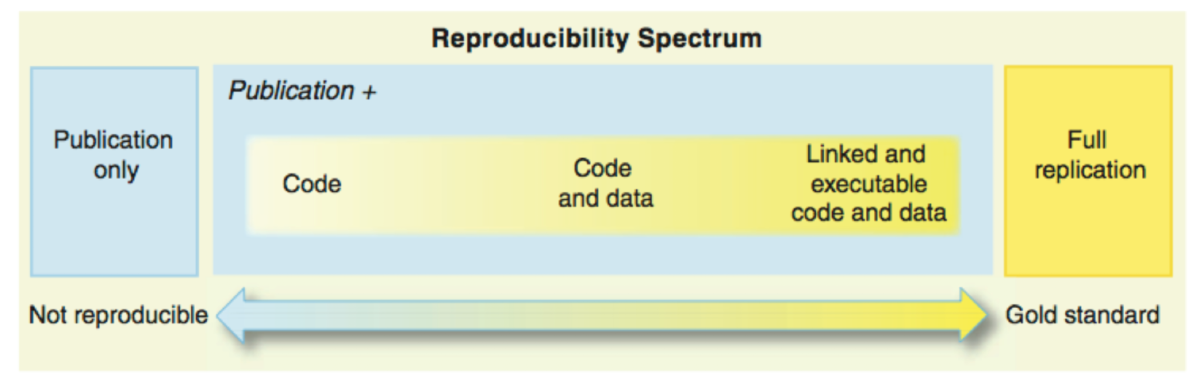
\includegraphics[width=1\linewidth,height=\textheight,keepaspectratio]{images/reproducibility.png}}

For mass communication researchers, this capability ensures transparency and integrity, which are particularly important when dealing with potentially sensitive or high-impact media data. Whether publishing a report on social media trends or presenting findings on audience demographics, R and RStudio help researchers document and share their work in a way that is fully traceable.

\subsection*{Flexibility and Customization}\label{flexibility-and-customization}
\addcontentsline{toc}{subsection}{Flexibility and Customization}

R's flexibility is one of its standout features. Unlike other statistical software, which may be limited by pre-built functions or rigid workflows, R allows users to customize their analyses by writing their own scripts. This adaptability is crucial in mass communication research, where the types of data (e.g., textual data, video metrics, user interactions) can vary widely and often require bespoke approaches.

Additionally, R's package system allows for almost limitless customization. Users can download packages specific to their field of research or even create their own, making it easier to tailor the analysis to the exact needs of a project. For example, mass communication researchers studying digital engagement might use packages designed for sentiment analysis, network visualization, or web scraping, all of which are readily available in the R ecosystem.

\section{How to Install R and RStudio}\label{how-to-install-r-and-rstudio}

R and RStudio are essential tools for data analysis, visualization, and reproducible research. This section will guide you through the steps to install both R and RStudio on your computer, ensuring you are ready to start coding and analyzing data efficiently.

\subsection*{How to Install R}\label{how-to-install-r}
\addcontentsline{toc}{subsection}{How to Install R}

R can be downloaded from the Comprehensive R Archive Network (CRAN) at \url{https://cran.r-project.org/}. Follow the steps below to install R on your machine:

\begin{enumerate}
\def\labelenumi{\arabic{enumi}.}
\tightlist
\item
  \textbf{Visit the CRAN website}: Navigate to \url{https://cran.r-project.org/}.
\item
  \textbf{Select your operating system}: Choose the appropriate option for your computer---Windows, Mac, or Linux.

  \begin{itemize}
  \tightlist
  \item
    \textbf{Windows}: Click on ``Download R for Windows,'' and then choose ``base'' to download the most recent version. Follow the installation prompts.
  \item
    \textbf{Mac}: Click on ``Download R for macOS,'' and choose the version compatible with your operating system. Follow the installation prompts.
  \item
    \textbf{Linux}: Select ``Download R for Linux'' and follow the specific instructions for your Linux distribution (e.g., Ubuntu, Debian, Fedora).
  \end{itemize}
\item
  \textbf{Complete the installation}: Once the download is complete, open the installer and follow the on-screen instructions to complete the installation. After installation, R should be ready to use on your system.
\end{enumerate}

\href{https://cran.r-project.org/}{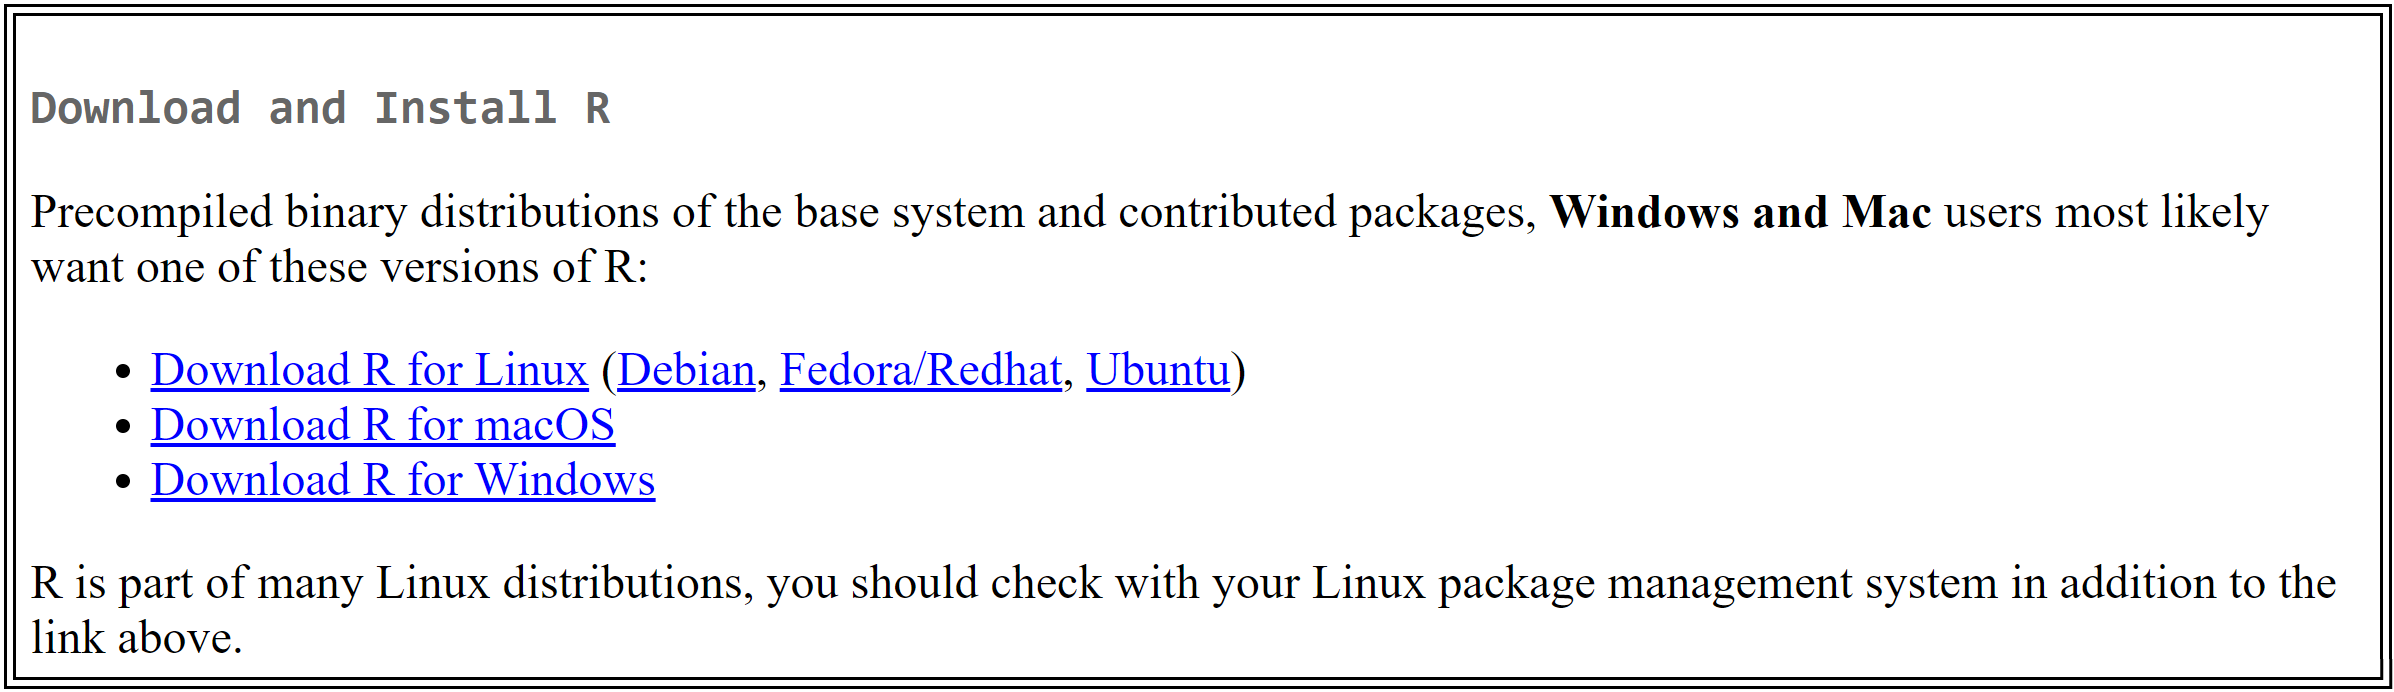
\includegraphics[width=1\linewidth,height=\textheight,keepaspectratio]{images/install-r.png}}

\subsection*{How to Install RStudio}\label{how-to-install-rstudio}
\addcontentsline{toc}{subsection}{How to Install RStudio}

After installing R, you need to install RStudio, a powerful Integrated Development Environment (IDE) that enhances your coding experience and workflow. Follow the steps below to install RStudio:

\begin{enumerate}
\def\labelenumi{\arabic{enumi}.}
\tightlist
\item
  \textbf{Visit the RStudio download page}: Go to \url{https://posit.co/download/rstudio-desktop/}.
\end{enumerate}

\href{https://posit.co/download/rstudio-desktop/}{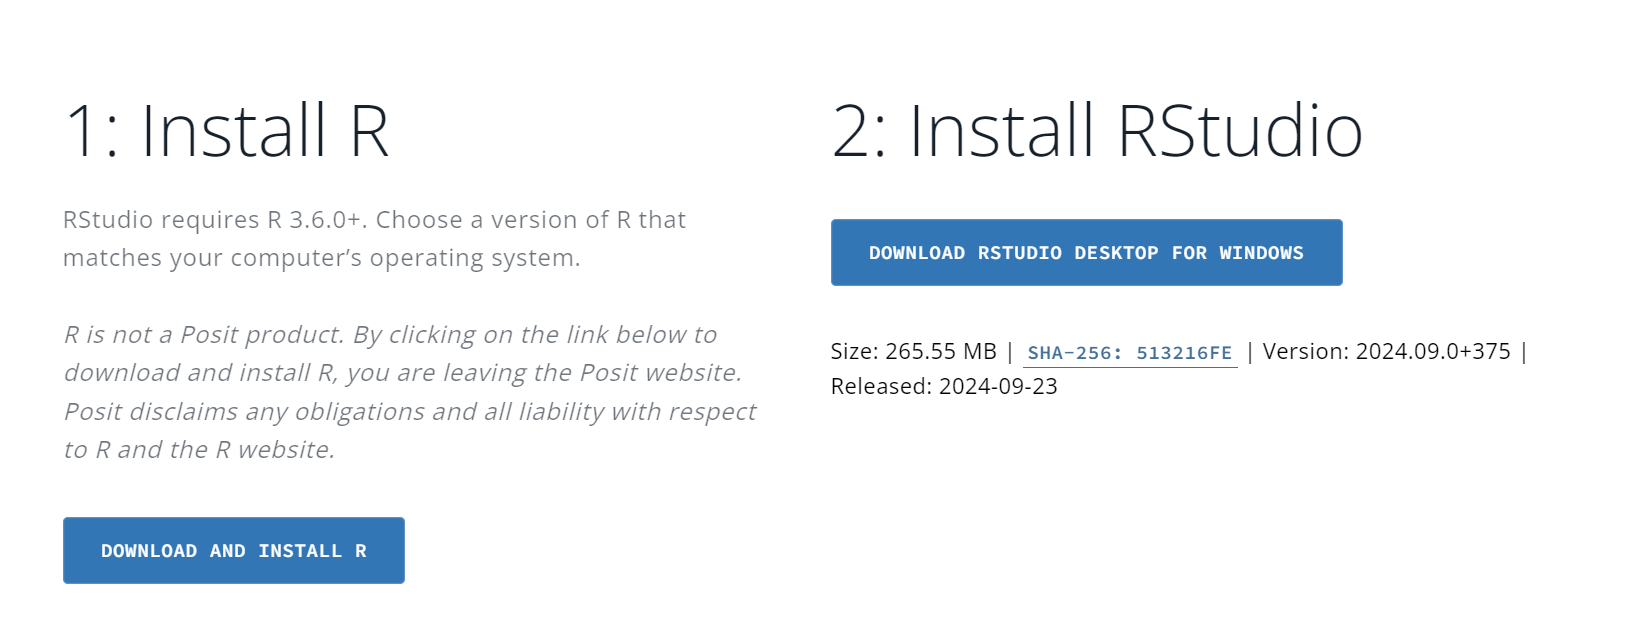
\includegraphics[width=1\linewidth,height=\textheight,keepaspectratio]{images/r-studio.png}}

\begin{enumerate}
\def\labelenumi{\arabic{enumi}.}
\setcounter{enumi}{1}
\tightlist
\item
  \textbf{Choose the free version}: Select ``RStudio Desktop -- Open Source License'' to download the free version of RStudio.
\item
  \textbf{Select your operating system}: Choose the installer for your operating system (Windows, Mac, or Linux) and download the appropriate file.

  \begin{itemize}
  \tightlist
  \item
    \textbf{Windows}: Download the installer and run it. Follow the setup prompts to install RStudio.
  \item
    \textbf{Mac}: Download the installer for macOS, open the .dmg file, and drag RStudio into your Applications folder.
  \item
    \textbf{Linux}: Follow the instructions provided on the RStudio download page for your specific Linux distribution.
  \end{itemize}
\item
  \textbf{Launch RStudio}: After installation, open RStudio. You should see the RStudio interface with the console panel, ready for you to start writing and running R code.
\end{enumerate}

\section{Getting Started with R and RStudio}\label{getting-started-with-r-and-rstudio}

\subsection*{The RStudio Interface}\label{the-rstudio-interface}
\addcontentsline{toc}{subsection}{The RStudio Interface}

RStudio enhances the R experience by providing a user-friendly interface that simplifies coding, analysis, and visualization. The workspace is divided into four main panels, each serving a distinct function:

\begin{itemize}
\tightlist
\item
  \textbf{Script Panel:} The script panel is where you write and edit your R scripts. Scripts are collections of commands that can be saved and reused, which promotes reproducibility and efficiency in your research. By saving your code as scripts, you can run the same analysis on different datasets or share the exact steps with collaborators.
\end{itemize}

\begin{figure}
\centering
\includegraphics[width=1\linewidth,height=\textheight,keepaspectratio]{images/script-panel.png}
\caption{Script Panel with iPlastic Theme}
\end{figure}

\begin{itemize}
\tightlist
\item
  \textbf{Console Panel:} The console is the interactive component where R executes commands. You can type commands directly into the console or run them from a script. The console also displays output, including error messages and other system feedback. This real-time interaction is helpful for testing snippets of code before integrating them into your larger script.
\end{itemize}

\begin{figure}
\centering
\includegraphics[width=1\linewidth,height=\textheight,keepaspectratio]{images/console-panel.png}
\caption{Console Panel with iPlastic Theme}
\end{figure}

\begin{itemize}
\tightlist
\item
  \textbf{Environment Panel:} The environment panel displays all the objects---such as datasets, variables, and functions---currently stored in memory during your R session. It provides an overview of the data and variables you are working with, allowing you to inspect, remove, or modify them easily.
\end{itemize}

\begin{figure}
\centering
\includegraphics[width=1\linewidth,height=\textheight,keepaspectratio]{images/environment-panel.png}
\caption{Environment Panel with iPlastic Theme}
\end{figure}

\begin{itemize}
\tightlist
\item
  \textbf{Plots/Help/Files Panels:} This multifunctional area is where RStudio displays generated plots and visualizations. It also gives access to R's extensive help files and documentation, helping users troubleshoot or learn about specific functions. Additionally, the file browser in this panel lets you navigate your computer's files and directories, making it easy to locate and import data into R.
\end{itemize}

\begin{figure}
\centering
\includegraphics[width=1\linewidth,height=\textheight,keepaspectratio]{images/files-panel.png}
\caption{Plots/Help/Files Panel with iPlastic Theme}
\end{figure}

\subsection*{Setting Up a New Project}\label{setting-up-a-new-project}
\addcontentsline{toc}{subsection}{Setting Up a New Project}

RStudio's project management system helps keep your work organized, especially when handling multiple files or analyses. Setting up a project ensures that all related files, scripts, and outputs are in one place.

\begin{itemize}
\tightlist
\item
  \textbf{Creating a Project:} To start a new project, go to \texttt{File\ \textgreater{}\ New\ Project...}. RStudio allows you to group all the scripts, data files, and visual outputs related to a specific research question or analysis into one project, making it easier to manage your workflow.
\end{itemize}

\begin{figure}
\centering
\includegraphics[width=1\linewidth,height=\textheight,keepaspectratio]{images/new-project.jpg}
\caption{New Project Menu}
\end{figure}

\begin{itemize}
\item
  \textbf{Choosing a Location:} You can create a new directory for your project or associate it with an existing folder. Creating projects within dedicated directories is crucial for managing your work, as it ensures all related files are in one location and that relative file paths are maintained. This makes it easier to share your project with others or run it on a different machine without breaking file links.
\item
  \textbf{Version Control:} If you use version control tools like Git, RStudio seamlessly integrates with them. During the project setup, you can create or link a Git repository, allowing you to track changes and collaborate with others effectively. Version control ensures that every modification to your scripts is documented, which is especially useful when working in teams.
\item
  \textbf{Project Management:} RStudio projects save the state of your workspace, including open files, console history, and the working directory. When you reopen the project, RStudio restores this state, enabling you to continue where you left off without needing to reconfigure your environment.
\end{itemize}

\subsection*{File Management}\label{file-management}
\addcontentsline{toc}{subsection}{File Management}

Effective file management is critical for maintaining an organized and efficient workflow in RStudio. Below are some guidelines for managing different types of files:

\subsubsection*{R Script vs.~R Markdown}\label{r-script-vs.-r-markdown}
\addcontentsline{toc}{subsubsection}{R Script vs.~R Markdown}

R scripts (\texttt{.R} files) are text files where you can write and run R commands. These are best used when the focus is purely on data analysis. On the other hand, R Markdown (\texttt{.Rmd} files) allows you to integrate narrative text, R code, and output (e.g., plots, tables) into a single document. R Markdown is useful for generating reproducible reports, making it ideal for assignments, papers, and presentations.

\begin{itemize}
\tightlist
\item
  \textbf{When to use R Script}: Use an R script when you are solely focused on coding and analyzing data without needing additional explanation or documentation.
\item
  \textbf{When to use R Markdown}: Use R Markdown when you want to combine text, code, and results in a report format that can be converted into HTML, PDF, or Word documents.
\end{itemize}

\begin{figure}
\centering
\includegraphics[width=1\linewidth,height=\textheight,keepaspectratio]{images/script-md.jpg}
\caption{R Script on Left and R Markdown on Right}
\end{figure}

\subsubsection*{CSV vs.~Excel}\label{csv-vs.-excel}
\addcontentsline{toc}{subsubsection}{CSV vs.~Excel}

For most data analysis tasks in R, \textbf{CSV} (Comma Separated Values) files are the preferred format due to their simplicity and compatibility with R's data manipulation functions. R also provides tools for reading \textbf{Excel} files (\texttt{.xlsx}), but Excel files often introduce complexities, such as multiple sheets or hidden formatting, which can complicate data analysis.

\begin{itemize}
\tightlist
\item
  \textbf{Use CSV files} for straightforward, clean datasets that will be frequently used in your analysis.
\item
  \textbf{Use Excel files} when working with collaborators who require Excel formatting or when the dataset contains multiple sheets or more complex structure.
\end{itemize}

\subsubsection*{Subfolders}\label{subfolders}
\addcontentsline{toc}{subsubsection}{Subfolders}

When working on large projects, use subfolders within your project directory to organize your files. Common subfolders might include: - \texttt{data/} for storing raw and processed datasets. - \texttt{scripts/} for organizing your R scripts. - \texttt{output/} for saving graphs, tables, and other generated outputs. - \texttt{reports/} for storing R Markdown files or other documents that summarize your findings.

This hierarchical organization makes it easier to locate files and ensures that your project remains structured as it grows in complexity.

\subsubsection*{Other Files}\label{other-files}
\addcontentsline{toc}{subsubsection}{Other Files}

In addition to scripts and datasets, you may work with a variety of other file types, such as: - \textbf{Text files (\texttt{.txt})} for plain text data. - \textbf{Image files (\texttt{.png}, \texttt{.jpeg})} for embedding visualizations or outputs into reports. - \textbf{RData files (\texttt{.RData})} for saving your R workspace so you can quickly reload objects in future sessions.

By keeping your files organized and labeled consistently, you can streamline your workflow and reduce the likelihood of errors when collaborating or revisiting older projects.

\section{Package Management}\label{package-management}

R's strength lies in its extensive ecosystem of packages, which extend its core functionality to support specific types of analysis, visualization, and data manipulation. Packages are collections of R functions, data, and documentation, tailored for different tasks. In mass communication research, several packages can aid in content analysis, media trend studies, and social network analysis.

\subsection*{Installing Packages}\label{installing-packages}
\addcontentsline{toc}{subsection}{Installing Packages}

To install a package in R, you need to use the \texttt{install.packages()} function. This only needs to be done once per package:

\begin{Shaded}
\begin{Highlighting}[]
\FunctionTok{install.packages}\NormalTok{(}\StringTok{"ggplot2"}\NormalTok{)}
\end{Highlighting}
\end{Shaded}

In RStudio, you can run this code in a code chunk or type it directly into the console. For example, to install a package in R Markdown, use the following code chunk:

\begin{Shaded}
\begin{Highlighting}[]
\FunctionTok{install.packages}\NormalTok{(}\StringTok{"ggplot2"}\NormalTok{)}
\end{Highlighting}
\end{Shaded}

After installation, load the package into your R session using the \texttt{library()} function:

\begin{Shaded}
\begin{Highlighting}[]
\FunctionTok{library}\NormalTok{(ggplot2)}
\end{Highlighting}
\end{Shaded}

This makes the package's functions available for use during your R session.

\subsection*{Commonly Used Packages}\label{commonly-used-packages}
\addcontentsline{toc}{subsection}{Commonly Used Packages}

Some packages particularly useful for mass communication research include: - \textbf{\texttt{ggplot2}}: For creating high-quality data visualizations. - \textbf{\texttt{dplyr}}: For data manipulation and cleaning. - \textbf{\texttt{tm}}: For text mining and content analysis, useful for analyzing media content. - \textbf{\texttt{rtweet}}: For collecting and analyzing Twitter data, essential in social media research. - \textbf{\texttt{quanteda}}: For text analysis, commonly used for media content studies.

Once installed, packages can be updated periodically using the \texttt{update.packages()} function.

\section{Basics of R Programming}\label{basics-of-r-programming}

This section introduces basic R programming concepts relevant to mass communication research. We assume no prior knowledge of coding, so we'll start from scratch. The examples below are designed to be used in R Markdown, which allows you to combine code, text, and output into a single, reproducible document.

\subsection*{Code Chunks in R Markdown}\label{code-chunks-in-r-markdown}
\addcontentsline{toc}{subsection}{Code Chunks in R Markdown}

In R Markdown, code is written inside ``chunks.'' These chunks execute code and display the output directly in the document. To insert a code chunk in R Markdown, use three backticks followed by \texttt{\{r\}} to indicate you are writing R code. For example:

\begin{Shaded}
\begin{Highlighting}[]
\CommentTok{\# This is a code chunk}
\FunctionTok{print}\NormalTok{(}\StringTok{"Hello, World!"}\NormalTok{)}
\end{Highlighting}
\end{Shaded}

\emph{Output: ``Hello, World!''}

The code inside the chunk runs when you ``knit'' the document, and the output will appear in the resulting file.

\subsection*{Manually Inputting Data}\label{manually-inputting-data}
\addcontentsline{toc}{subsection}{Manually Inputting Data}

Data can be input directly into R, which is useful for small datasets or examples. Below is how you manually input data as a vector (a list of numbers or words):

\begin{Shaded}
\begin{Highlighting}[]
\CommentTok{\# Inputting numerical data}
\NormalTok{age }\OtherTok{\textless{}{-}} \FunctionTok{c}\NormalTok{(}\DecValTok{18}\NormalTok{, }\DecValTok{23}\NormalTok{, }\DecValTok{21}\NormalTok{, }\DecValTok{30}\NormalTok{)}

\CommentTok{\# Inputting character data}
\NormalTok{names }\OtherTok{\textless{}{-}} \FunctionTok{c}\NormalTok{(}\StringTok{"Alice"}\NormalTok{, }\StringTok{"Bob"}\NormalTok{, }\StringTok{"Carol"}\NormalTok{, }\StringTok{"David"}\NormalTok{)}
\end{Highlighting}
\end{Shaded}

\section{Commenting and Organizing Code}\label{commenting-and-organizing-code}

Clear, well-commented, and organized code is crucial for making your analysis reproducible and understandable, especially when sharing it with others or revisiting it later.

\subsection*{Commenting Code}\label{commenting-code}
\addcontentsline{toc}{subsection}{Commenting Code}

In R, comments are created using the \texttt{\#} symbol. Anything written after \texttt{\#} is ignored by R and is only meant for humans reading the code. Commenting is useful for explaining what each section of the code does or noting important details about the analysis:

\begin{Shaded}
\begin{Highlighting}[]
\CommentTok{\# This is a comment}
\NormalTok{age }\OtherTok{\textless{}{-}} \FunctionTok{c}\NormalTok{(}\DecValTok{18}\NormalTok{, }\DecValTok{23}\NormalTok{, }\DecValTok{21}\NormalTok{, }\DecValTok{30}\NormalTok{)  }\CommentTok{\# Vector of ages}
\end{Highlighting}
\end{Shaded}

Use comments to explain the purpose of code sections, especially when performing key analyses. For example:

\begin{Shaded}
\begin{Highlighting}[]
\CommentTok{\# This code reads data from an online CSV file}
\NormalTok{billboard }\OtherTok{\textless{}{-}} \FunctionTok{read.csv}\NormalTok{(}\StringTok{"https://raw.githubusercontent.com/rfordatascience/tidytuesday/refs/heads/master/data/2021/2021{-}09{-}14/billboard.csv"}\NormalTok{)}
\end{Highlighting}
\end{Shaded}

\subsection*{Organizing Code with Sections}\label{organizing-code-with-sections}
\addcontentsline{toc}{subsection}{Organizing Code with Sections}

To organize larger scripts, you can use headers or dividers to mark different sections. This makes it easier to navigate the code:

\begin{Shaded}
\begin{Highlighting}[]
\CommentTok{\# ===========================}
\CommentTok{\# Section: Data Preparation}
\CommentTok{\# ===========================}
\end{Highlighting}
\end{Shaded}

In R Markdown, you can organize code sections using headings in markdown format:

\section{Data Preparation}\label{data-preparation}

\begin{Shaded}
\begin{Highlighting}[]
\CommentTok{\# Code for preparing data goes here}
\end{Highlighting}
\end{Shaded}

\subsection*{Keeping Code Tidy}\label{keeping-code-tidy}
\addcontentsline{toc}{subsection}{Keeping Code Tidy}

Organized, readable code is essential, especially in collaborative research projects. Some tips for keeping your code tidy: - Use consistent indentation for better readability. - Break long lines of code into multiple lines. - Avoid excessive nesting of functions; instead, break them into separate steps.

By commenting effectively and organizing your code logically, you make it easier for others (and yourself) to understand your analysis, contributing to better research practices.

\section{Basic Operations in R}\label{basic-operations-in-r}

Understanding the basic operations in R is vital for embarking on more complex data analysis and programming tasks. These operations include arithmetic calculations, variable assignments, and function calls.

\subsection*{Arithmetic Operations}\label{arithmetic-operations}
\addcontentsline{toc}{subsection}{Arithmetic Operations}

\subsubsection*{Overview}\label{overview}
\addcontentsline{toc}{subsubsection}{Overview}

Arithmetic operations form the basis of numerical calculations in R. These operations can be conducted directly in the R console and include addition, subtraction, multiplication, division, exponentiation, and other mathematical functions (Chambers, 2008).

\subsubsection*{Common Arithmetic Operators}\label{common-arithmetic-operators}
\addcontentsline{toc}{subsubsection}{Common Arithmetic Operators}

\begin{itemize}
\tightlist
\item
  \textbf{Addition (\texttt{+})}: Adds two numbers.
\item
  \textbf{Subtraction (\texttt{-})}: Subtracts the right-hand operand from the left-hand operand.
\item
  \textbf{Multiplication (\texttt{*})}: Multiplies two numbers.
\item
  \textbf{Division (\texttt{/})}: Divides the left-hand operand by the right-hand operand.
\item
  \textbf{Exponentiation (\texttt{\^{}})}: Raises the left-hand operand to the power of the right-hand operand.
\item
  \textbf{Modulus (\texttt{\%\%})}: Gives the remainder of the division between two numbers.
\end{itemize}

\subsubsection*{Examples}\label{examples}
\addcontentsline{toc}{subsubsection}{Examples}

You can execute these basic arithmetic operations directly in the R console.

\textbf{\emph{Addition}}

\begin{Shaded}
\begin{Highlighting}[]
\DecValTok{5} \SpecialCharTok{+} \DecValTok{3}
\end{Highlighting}
\end{Shaded}

\emph{Output: 8}

\textbf{\emph{Subtraction}}

\begin{Shaded}
\begin{Highlighting}[]
\DecValTok{5} \SpecialCharTok{{-}} \DecValTok{3}
\end{Highlighting}
\end{Shaded}

\emph{Output: 2}

\textbf{\emph{Multiplication}}

\begin{Shaded}
\begin{Highlighting}[]
\DecValTok{5} \SpecialCharTok{*} \DecValTok{3}
\end{Highlighting}
\end{Shaded}

\emph{Output: 15}

\textbf{\emph{Division}}

\begin{Shaded}
\begin{Highlighting}[]
\DecValTok{5} \SpecialCharTok{/} \DecValTok{3}
\end{Highlighting}
\end{Shaded}

\emph{Output: 1.666667}

\textbf{\emph{Exponentiation}}

\begin{Shaded}
\begin{Highlighting}[]
\DecValTok{5} \SpecialCharTok{\^{}} \DecValTok{3}
\end{Highlighting}
\end{Shaded}

\emph{Output: 125}

\subsection*{Variables}\label{variables}
\addcontentsline{toc}{subsection}{Variables}

\subsubsection*{What Are Variables?}\label{what-are-variables}
\addcontentsline{toc}{subsubsection}{What Are Variables?}

Variables act as storage containers for data, including numbers, strings, vectors, and other complex data types. Variable assignment is a crucial aspect of programming and data management in R (Wickham, 2014).

\subsubsection*{Assignment Operators}\label{assignment-operators}
\addcontentsline{toc}{subsubsection}{Assignment Operators}

\begin{itemize}
\tightlist
\item
  \textbf{Leftward (\texttt{\textless{}-})}: Assigns the value on the right to the variable on the left.
\item
  \textbf{Equal (\texttt{=})}: Can also be used for assignment, though \texttt{\textless{}-} is traditionally preferred in R.
\end{itemize}

\subsubsection*{Examples}\label{examples-1}
\addcontentsline{toc}{subsubsection}{Examples}

\begin{Shaded}
\begin{Highlighting}[]
\CommentTok{\# Assigning a numerical value to a variable using \textless{}{-}}
\NormalTok{x }\OtherTok{\textless{}{-}} \DecValTok{10}
\NormalTok{y }\OtherTok{\textless{}{-}} \DecValTok{20}

\CommentTok{\# Assigning a string value to a variable using =}
\NormalTok{text\_variable }\OtherTok{=} \StringTok{"Hello, World!"}

\CommentTok{\# Printing variables}
\FunctionTok{print}\NormalTok{(x)}
\FunctionTok{print}\NormalTok{(text\_variable)}
\end{Highlighting}
\end{Shaded}

\emph{Output:10} \emph{``Hello, World!''}

\subsection*{Functions}\label{functions}
\addcontentsline{toc}{subsection}{Functions}

\subsubsection*{Function Overview}\label{function-overview}
\addcontentsline{toc}{subsubsection}{Function Overview}

Functions are predefined sets of operations that perform specific tasks. Functions in R can be either built-in, such as \texttt{sum()} or \texttt{mean()}, or user-defined for more customized operations (Chambers, 2008).

\subsubsection*{Built-in Functions}\label{built-in-functions}
\addcontentsline{toc}{subsubsection}{Built-in Functions}

Examples of common built-in functions include: dz - \textbf{\texttt{sum()}}: Calculates the sum of all the values in a numeric vector. - \textbf{\texttt{mean()}}: Calculates the arithmetic mean of a numeric vector. - \textbf{\texttt{sqrt()}}: Calculates the square root of a number.

\textbf{\emph{Using sum function}}

\begin{Shaded}
\begin{Highlighting}[]
\FunctionTok{sum}\NormalTok{(}\DecValTok{1}\NormalTok{, }\DecValTok{2}\NormalTok{, }\DecValTok{3}\NormalTok{)}
\end{Highlighting}
\end{Shaded}

\emph{Output: 6}

\textbf{\emph{Using mean function}}

\begin{Shaded}
\begin{Highlighting}[]
\FunctionTok{mean}\NormalTok{(}\FunctionTok{c}\NormalTok{(}\DecValTok{1}\NormalTok{, }\DecValTok{2}\NormalTok{, }\DecValTok{3}\NormalTok{, }\DecValTok{4}\NormalTok{))}
\end{Highlighting}
\end{Shaded}

\emph{Output: 2.5}

\textbf{\emph{Using sqrt function}}

\begin{Shaded}
\begin{Highlighting}[]
\FunctionTok{sqrt}\NormalTok{(}\DecValTok{16}\NormalTok{)}
\end{Highlighting}
\end{Shaded}

\emph{Output: 4}

\chapter{Data Management}\label{data-management}

\href{_book/files/09-data_management-chunks.Rmd}{{[}Chunk Version{]}}

\section{Defining Data}\label{defining-data}

\subsection*{What is Data?}\label{what-is-data}
\addcontentsline{toc}{subsection}{What is Data?}

In research, data refers to information collected to answer questions, test hypotheses, or explore patterns. Data can take many forms---numbers, text, or categories---and understanding these forms is essential for effective analysis. In RStudio, data is organized in tables called \textbf{data frames}, where rows represent individual observations and columns represent variables.

\subsection*{What is Data in Mass Communication Research?}\label{what-is-data-in-mass-communication-research}
\addcontentsline{toc}{subsection}{What is Data in Mass Communication Research?}

In mass communication research, data often comes from audience surveys, digital platforms, gaming environments, or content analyses. The \textbf{\texttt{gaming-anxiety.csv}} dataset is an example of survey data collected from gamers, which includes psychological scale responses (e.g., anxiety, satisfaction with life), game behaviors (e.g., hours played, streaming frequency), and demographics (e.g., age, gender, location). These data can be used to study relationships between psychological well-being and gaming behavior.

\subsection*{Qualitative vs.~Quantitative Data}\label{qualitative-vs.-quantitative-data}
\addcontentsline{toc}{subsection}{Qualitative vs.~Quantitative Data}

In the \textbf{\texttt{gaming-anxiety.csv}} dataset, variables can be classified as either qualitative or quantitative.

\begin{itemize}
\item
  \textbf{Qualitative Data}: Qualitative data are non-numerical and typically describe categories or characteristics. In this dataset, \texttt{Game}, \texttt{Platform}, \texttt{Playstyle}, and \texttt{Gender} are qualitative variables. These variables describe how respondents play games or how they identify, without involving numeric values.
\item
  \textbf{Quantitative Data}: Quantitative data are numerical and allow for statistical analysis. In this dataset, variables such as \texttt{Age}, \texttt{Hours} (spent gaming per week), \texttt{GAD1} to \texttt{GAD7} (General Anxiety Disorder items), and \texttt{SWL1} to \texttt{SWL5} (Satisfaction With Life items) are quantitative. These values allow researchers to calculate scores and identify patterns in gamer well-being.
\end{itemize}

\section{Variables and Observations}\label{variables-and-observations}

In RStudio, datasets are displayed in tabular format where \textbf{columns represent variables} and \textbf{rows represent observations}.

\begin{itemize}
\item
  \textbf{Variables}: Variables are measurable characteristics or data fields. In the \texttt{gaming-anxiety.csv} dataset, variables include \texttt{Age}, \texttt{Game}, \texttt{GAD1}, \texttt{SWL2}, and \texttt{SPIN\_T}. Each variable corresponds to a different question or category from the survey. For example, \texttt{GAD1} records how often a respondent felt nervous, while \texttt{Platform} indicates their gaming device.
\item
  \textbf{Observations}: Observations are the individual entries or survey responses. Each row in \texttt{gaming-anxiety.csv} represents one gamer's full set of responses, including their psychological scores, gaming behavior, and demographic information. These are the units of analysis.
\end{itemize}

\subsection*{Explanation of Data Types}\label{explanation-of-data-types}
\addcontentsline{toc}{subsection}{Explanation of Data Types}

The dataset includes a variety of data types, each requiring different analytical techniques:

\begin{itemize}
\item
  \textbf{Nominal Data}: These are unordered categories. For example, \texttt{Game}, \texttt{Gender}, and \texttt{Platform} are nominal because they describe types without implying rank.
\item
  \textbf{Ordinal Data}: These categories have a logical order. While not directly labeled as such, variables like \texttt{highestleague} or Likert-scale items (e.g., from the \texttt{whyplay} or \texttt{GADE} questions) might represent ordinal responses, depending on how the data were collected.
\item
  \textbf{Discrete Data}: Discrete numeric data are countable and often whole numbers. Variables such as \texttt{streams} (number of times streamed) and \texttt{SPIN\_T} (Social Phobia Inventory total score) are discrete because they represent count-based values.
\item
  \textbf{Continuous Data}: These are numeric values that can take any value in a range. \texttt{Hours} (hours spent gaming per week) and \texttt{Age} are continuous, as they represent measurements that can vary on a spectrum.
\item
  \textbf{Dichotomous or Binary Data}: These variables have only two values (e.g., Yes/No, Accept/Reject). In this dataset, \texttt{accept} is an example of a dichotomous variable indicating whether the participant accepted the terms of the study.
\end{itemize}

\section{Inputting Data}\label{inputting-data}

In RStudio, entering or importing data is an essential first step in any research project. Most datasets, like \texttt{gaming-anxiety.csv}, come in \textbf{CSV (comma-separated values)} format, which can be easily read into R using functions like \texttt{read\_csv()} from the \texttt{readr} package.

\subsection*{Data Structures in R}\label{data-structures-in-r}
\addcontentsline{toc}{subsection}{Data Structures in R}

Data structures are fundamental in R programming as they organize and store the data that one works with for analyses, visualizations, and other computational tasks. Understanding these structures is critical for effective manipulation of data and implementing various algorithms (Wickham \& Grolemund, 2017). Below are the primary data structures that R provides.

\subsubsection*{Vectors}\label{vectors}
\addcontentsline{toc}{subsubsection}{Vectors}

Vectors are one-dimensional arrays used to hold elements of a single data type. This could be numeric, character, or logical data types. Vectors are often used for operations that require the application of a function to each element in the data set (Maindonald \& Braun, 2010).

Vectors can be created using the \texttt{c()} function, which combines elements into a vector.

\emph{Creating a numeric vector}

\begin{Shaded}
\begin{Highlighting}[]
\NormalTok{numeric\_vector }\OtherTok{\textless{}{-}} \FunctionTok{c}\NormalTok{(}\DecValTok{1}\NormalTok{, }\DecValTok{2}\NormalTok{, }\DecValTok{3}\NormalTok{, }\DecValTok{4}\NormalTok{, }\DecValTok{5}\NormalTok{)}
\end{Highlighting}
\end{Shaded}

\emph{Creating a character vector}

\begin{Shaded}
\begin{Highlighting}[]
\NormalTok{character\_vector }\OtherTok{\textless{}{-}} \FunctionTok{c}\NormalTok{(}\StringTok{"apple"}\NormalTok{, }\StringTok{"banana"}\NormalTok{, }\StringTok{"cherry"}\NormalTok{)}
\end{Highlighting}
\end{Shaded}

\emph{Creating a logical vector}

\begin{Shaded}
\begin{Highlighting}[]
\NormalTok{logical\_vector }\OtherTok{\textless{}{-}} \FunctionTok{c}\NormalTok{(}\ConstantTok{TRUE}\NormalTok{, }\ConstantTok{FALSE}\NormalTok{, }\ConstantTok{TRUE}\NormalTok{)}
\end{Highlighting}
\end{Shaded}

You can perform various operations on vectors like addition, subtraction, or applying a function to each element.

\begin{Shaded}
\begin{Highlighting}[]
\CommentTok{\# Adding two vectors}
\NormalTok{sum\_vector }\OtherTok{\textless{}{-}}\NormalTok{ numeric\_vector }\SpecialCharTok{+} \FunctionTok{c}\NormalTok{(}\DecValTok{1}\NormalTok{, }\DecValTok{1}\NormalTok{, }\DecValTok{1}\NormalTok{, }\DecValTok{1}\NormalTok{, }\DecValTok{1}\NormalTok{)}

\CommentTok{\# Calculating mean of a numeric vector}
\NormalTok{mean\_value }\OtherTok{\textless{}{-}} \FunctionTok{mean}\NormalTok{(numeric\_vector)}
\end{Highlighting}
\end{Shaded}

\subsubsection*{Data Frames}\label{data-frames}
\addcontentsline{toc}{subsubsection}{Data Frames}

Data frames serve as the fundamental data structure for data analysis in R. They are similar to matrices but allow different types of variables in different columns, which makes them extremely versatile (Chambers, 2008).

Data frames can be created using the \texttt{data.frame()} function.

\begin{Shaded}
\begin{Highlighting}[]
\CommentTok{\# Creating a data frame}
\NormalTok{df }\OtherTok{\textless{}{-}} \FunctionTok{data.frame}\NormalTok{(}\AttributeTok{Name =} \FunctionTok{c}\NormalTok{(}\StringTok{"Alice"}\NormalTok{, }\StringTok{"Bob"}\NormalTok{), }\AttributeTok{Age =} \FunctionTok{c}\NormalTok{(}\DecValTok{23}\NormalTok{, }\DecValTok{45}\NormalTok{), }\AttributeTok{Gender =} \FunctionTok{c}\NormalTok{(}\StringTok{"F"}\NormalTok{, }\StringTok{"M"}\NormalTok{))}
\end{Highlighting}
\end{Shaded}

Various operations like subsetting, merging, and sorting can be performed on data frames.

\begin{Shaded}
\begin{Highlighting}[]
\CommentTok{\# Subsetting data frame by column}
\NormalTok{subset\_df }\OtherTok{\textless{}{-}}\NormalTok{ df[, }\FunctionTok{c}\NormalTok{(}\StringTok{"Name"}\NormalTok{, }\StringTok{"Age"}\NormalTok{)]}
\end{Highlighting}
\end{Shaded}

\subsubsection*{Lists}\label{lists}
\addcontentsline{toc}{subsubsection}{Lists}

Lists are an ordered collection of objects, which can be of different types and structures, including vectors, matrices, and even other lists (Wickham \& Grolemund, 2017).

Lists can be created using the \texttt{list()} function.

\begin{Shaded}
\begin{Highlighting}[]
\CommentTok{\# Creating a list}
\NormalTok{my\_list }\OtherTok{\textless{}{-}} \FunctionTok{list}\NormalTok{(}\AttributeTok{Name =} \StringTok{"Alice"}\NormalTok{, }\AttributeTok{Age =} \DecValTok{23}\NormalTok{, }\AttributeTok{Scores =} \FunctionTok{c}\NormalTok{(}\DecValTok{90}\NormalTok{, }\DecValTok{85}\NormalTok{, }\DecValTok{88}\NormalTok{))}
\end{Highlighting}
\end{Shaded}

Lists can be modified by adding, deleting, or updating list elements.

\begin{Shaded}
\begin{Highlighting}[]
\CommentTok{\# Updating a list element}
\NormalTok{my\_list}\SpecialCharTok{$}\NormalTok{Name }\OtherTok{\textless{}{-}} \StringTok{"Bob"}

\CommentTok{\# Adding a new list element}
\NormalTok{my\_list}\SpecialCharTok{$}\NormalTok{Email }\OtherTok{\textless{}{-}} \StringTok{"bob@email.com"}
\end{Highlighting}
\end{Shaded}

By understanding these primary data structures, students in Mass Communications can gain a strong foundation for more complex data analyses relevant to their field, whether it involves analyzing large sets of textual data, audience metrics, or other forms of media data.

\subsection*{Importing Data from a File}\label{importing-data-from-a-file}
\addcontentsline{toc}{subsection}{Importing Data from a File}

When working with larger datasets, such as CSV files, importing data into R is more efficient. A CSV (Comma Separated Values) file stores tabular data as plain text, making it easy to exchange data between programs. Below are several ways to import the \textbf{gaming-anxiety.csv} dataset into R.

\subsubsection*{\texorpdfstring{Use \texttt{read.csv} from Base R}{Use read.csv from Base R}}\label{use-read.csv-from-base-r}
\addcontentsline{toc}{subsubsection}{Use \texttt{read.csv} from Base R}

The \texttt{read.csv()} function is part of base R and can be used to import CSV files directly into your environment:

\begin{Shaded}
\begin{Highlighting}[]
\CommentTok{\# Reading the IMDb\_Economist\_tv\_ratings dataset using read.csv from base R}
\NormalTok{csv\_base }\OtherTok{\textless{}{-}} \FunctionTok{read.csv}\NormalTok{(}\StringTok{"https://github.com/SIM{-}Lab{-}SIUE/SIM{-}Lab{-}SIUE.github.io/raw/refs/heads/main/research{-}methods/data/gaming{-}anxiety.csv"}\NormalTok{, }\AttributeTok{header =} \ConstantTok{TRUE}\NormalTok{, }\AttributeTok{stringsAsFactors =} \ConstantTok{FALSE}\NormalTok{)}
\end{Highlighting}
\end{Shaded}

This code imports the dataset from the URL provided. The \texttt{header\ =\ TRUE} argument indicates that the first row contains variable names, and \texttt{stringsAsFactors\ =\ FALSE} prevents character strings from being converted to factors.

Use \texttt{write.csv()} to write a data frame to a csv.

\subsubsection*{\texorpdfstring{Use \texttt{read\_csv} from the \texttt{readr} Package}{Use read\_csv from the readr Package}}\label{use-read_csv-from-the-readr-package}
\addcontentsline{toc}{subsubsection}{Use \texttt{read\_csv} from the \texttt{readr} Package}

The \texttt{readr} package provides an alternative function, \texttt{read\_csv()}, which offers better performance and flexibility:

\begin{Shaded}
\begin{Highlighting}[]
\CommentTok{\# Install the readr package if it\textquotesingle{}s not already installed}
\CommentTok{\# install.packages("readr")}

\CommentTok{\# Load the readr package}
\FunctionTok{library}\NormalTok{(readr)}

\CommentTok{\# Reading the IMDb\_Economist\_tv\_ratings dataset using read\_csv from readr}
\NormalTok{csv\_readr }\OtherTok{\textless{}{-}} \FunctionTok{read\_csv}\NormalTok{(}\StringTok{"https://github.com/SIM{-}Lab{-}SIUE/SIM{-}Lab{-}SIUE.github.io/raw/refs/heads/main/research{-}methods/data/gaming{-}anxiety.csv"}\NormalTok{)}
\end{Highlighting}
\end{Shaded}

The \texttt{read\_csv()} function is faster than \texttt{read.csv()} and automatically detects data types, making it easier to handle larger datasets efficiently.

Use \texttt{write\_csv()} to write a data frame to a csv.

\subsubsection*{\texorpdfstring{Use \texttt{fread} from the \texttt{data.table} Package}{Use fread from the data.table Package}}\label{use-fread-from-the-data.table-package}
\addcontentsline{toc}{subsubsection}{Use \texttt{fread} from the \texttt{data.table} Package}

For very large datasets, \texttt{fread()} from the \texttt{data.table} package is a faster alternative:

\begin{Shaded}
\begin{Highlighting}[]
\CommentTok{\# Install the data.table package if it\textquotesingle{}s not already installed}
\CommentTok{\# install.packages("data.table")}

\CommentTok{\# Load the data.table package}
\FunctionTok{library}\NormalTok{(data.table)}

\CommentTok{\# Reading the IMDb\_Economist\_tv\_ratings dataset using fread from data.table}
\NormalTok{csv\_datatable }\OtherTok{\textless{}{-}} \FunctionTok{fread}\NormalTok{(}\StringTok{"https://github.com/SIM{-}Lab{-}SIUE/SIM{-}Lab{-}SIUE.github.io/raw/refs/heads/main/research{-}methods/data/gaming{-}anxiety.csv"}\NormalTok{)}
\end{Highlighting}
\end{Shaded}

The \texttt{fread()} function provides high-speed reading for large CSV files, making it ideal for processing extensive datasets.

Use \texttt{fwrite()} to write a data frame to a csv.

\subsubsection*{\texorpdfstring{Use \texttt{vroom,} from the \texttt{vroom} Package}{Use vroom, from the vroom Package}}\label{use-vroom-from-the-vroom-package}
\addcontentsline{toc}{subsubsection}{Use \texttt{vroom,} from the \texttt{vroom} Package}

The fastest method for reading rectangular data that I know of is \texttt{vroom()} from the \texttt{vroom} package:

\begin{Shaded}
\begin{Highlighting}[]
\CommentTok{\# Install the data.table package if it\textquotesingle{}s not already installed}
\CommentTok{\# install.packages("vroom")}

\CommentTok{\# Load the data.table package}
\FunctionTok{library}\NormalTok{(vroom)}

\CommentTok{\# Reading the IMDb\_Economist\_tv\_ratings dataset using fread from data.table}
\NormalTok{csv\_vroom }\OtherTok{\textless{}{-}} \FunctionTok{vroom}\NormalTok{(}\StringTok{"https://github.com/SIM{-}Lab{-}SIUE/SIM{-}Lab{-}SIUE.github.io/raw/refs/heads/main/research{-}methods/data/gaming{-}anxiety.csv"}\NormalTok{)}
\end{Highlighting}
\end{Shaded}

The \texttt{vroom()} function provides the fastest current read for .csv files.

Use \texttt{vroom\_write()} to write a data frame to a csv.

\section{Manipulating Data}\label{manipulating-data}

Data manipulation is a crucial aspect of preparing datasets for analysis. In RStudio, the \textbf{\texttt{dplyr}} package---part of the tidyverse ecosystem---provides powerful, intuitive functions for transforming, summarizing, and reshaping data. This section introduces \texttt{dplyr} and demonstrates how to manipulate data using examples from the \textbf{billboard} dataset, which contains information about songs, performers, and chart positions.

\subsection*{\texorpdfstring{The \texttt{dplyr} Package}{The dplyr Package}}\label{the-dplyr-package}
\addcontentsline{toc}{subsection}{The \texttt{dplyr} Package}

\subsubsection*{Introducing Tidyverse}\label{introducing-tidyverse}
\addcontentsline{toc}{subsubsection}{Introducing Tidyverse}

\textbf{Tidyverse} is a collection of R packages designed for data science, which share an underlying design philosophy and programming style. The \texttt{dplyr} package is part of the tidyverse and is widely used for data manipulation tasks such as filtering rows, selecting columns, grouping data, and summarizing statistics.

To get started, load the tidyverse (or specifically \texttt{dplyr}) into your R environment:

\begin{Shaded}
\begin{Highlighting}[]
\CommentTok{\# Load the dplyr package}
\FunctionTok{library}\NormalTok{(dplyr)}
\end{Highlighting}
\end{Shaded}

Load the \textbf{gaming\_anxiety} dataset from an online file

\begin{Shaded}
\begin{Highlighting}[]
\CommentTok{\# Load the data.table package}
\FunctionTok{library}\NormalTok{(}\StringTok{"data.table"}\NormalTok{)}

\CommentTok{\#@ Load the gaming\_anxiety dataset}
\NormalTok{gaming\_anxiety }\OtherTok{\textless{}{-}} \FunctionTok{fread}\NormalTok{(}\StringTok{"https://github.com/SIM{-}Lab{-}SIUE/SIM{-}Lab{-}SIUE.github.io/raw/refs/heads/main/research{-}methods/data/gaming{-}anxiety.csv"}\NormalTok{)}
\end{Highlighting}
\end{Shaded}

\subsubsection*{\texorpdfstring{The Pipe Operator \texttt{\%\textgreater{}\%}}{The Pipe Operator \%\textgreater\%}}\label{the-pipe-operator}
\addcontentsline{toc}{subsubsection}{The Pipe Operator \texttt{\%\textgreater{}\%}}

The pipe operator \texttt{\%\textgreater{}\%} passes the result of one function into the next. This allows you to build operations in readable, sequential steps.

Instead of:

\begin{Shaded}
\begin{Highlighting}[]
\FunctionTok{summarize}\NormalTok{(}\FunctionTok{group\_by}\NormalTok{(gaming\_anxiety, Gender), }\AttributeTok{avg\_age =} \FunctionTok{mean}\NormalTok{(Age, }\AttributeTok{na.rm =} \ConstantTok{TRUE}\NormalTok{))}
\end{Highlighting}
\end{Shaded}

Use:

\begin{Shaded}
\begin{Highlighting}[]
\NormalTok{gaming\_anxiety }\SpecialCharTok{\%\textgreater{}\%}
  \FunctionTok{group\_by}\NormalTok{(Gender) }\SpecialCharTok{\%\textgreater{}\%}
  \FunctionTok{summarize}\NormalTok{(}\AttributeTok{avg\_age =} \FunctionTok{mean}\NormalTok{(Age, }\AttributeTok{na.rm =} \ConstantTok{TRUE}\NormalTok{))}
\end{Highlighting}
\end{Shaded}

\subsubsection*{\texorpdfstring{Important \texttt{dplyr} Commands}{Important dplyr Commands}}\label{important-dplyr-commands}
\addcontentsline{toc}{subsubsection}{Important \texttt{dplyr} Commands}

\textbf{01. `summarize()}

Calculates summary statistics across the entire dataset or within groups.

\begin{Shaded}
\begin{Highlighting}[]
\NormalTok{gaming\_anxiety }\SpecialCharTok{\%\textgreater{}\%}
  \FunctionTok{summarize}\NormalTok{(}\AttributeTok{avg\_hours =} \FunctionTok{mean}\NormalTok{(Hours, }\AttributeTok{na.rm =} \ConstantTok{TRUE}\NormalTok{))}
\end{Highlighting}
\end{Shaded}

\textbf{02. `count()}

Counts the frequency of unique values in a column.

\begin{Shaded}
\begin{Highlighting}[]
\NormalTok{gaming\_anxiety }\SpecialCharTok{\%\textgreater{}\%}
  \FunctionTok{count}\NormalTok{(Platform)}
\end{Highlighting}
\end{Shaded}

\textbf{03. `group\_by()}

Groups data by one or more variables, typically followed by \texttt{summarize()} or \texttt{mutate()}.

\begin{Shaded}
\begin{Highlighting}[]
\NormalTok{gaming\_anxiety }\SpecialCharTok{\%\textgreater{}\%}
  \FunctionTok{group\_by}\NormalTok{(Gender) }\SpecialCharTok{\%\textgreater{}\%}
  \FunctionTok{summarize}\NormalTok{(}\AttributeTok{mean\_age =} \FunctionTok{mean}\NormalTok{(Age, }\AttributeTok{na.rm =} \ConstantTok{TRUE}\NormalTok{))}
\end{Highlighting}
\end{Shaded}

\textbf{04. `ungroup()}

Removes grouping structure after a grouped operation.

\begin{Shaded}
\begin{Highlighting}[]
\NormalTok{gaming\_anxiety }\SpecialCharTok{\%\textgreater{}\%}
  \FunctionTok{group\_by}\NormalTok{(Gender) }\SpecialCharTok{\%\textgreater{}\%}
  \FunctionTok{summarize}\NormalTok{(}\AttributeTok{mean\_age =} \FunctionTok{mean}\NormalTok{(Age, }\AttributeTok{na.rm =} \ConstantTok{TRUE}\NormalTok{)) }\SpecialCharTok{\%\textgreater{}\%}
  \FunctionTok{ungroup}\NormalTok{()}
\end{Highlighting}
\end{Shaded}

\textbf{05. `mutate()}

Creates new variables or modifies existing ones.

\begin{Shaded}
\begin{Highlighting}[]
\NormalTok{gaming\_anxiety }\SpecialCharTok{\%\textgreater{}\%}
  \FunctionTok{mutate}\NormalTok{(}\AttributeTok{hours\_per\_day =}\NormalTok{ Hours }\SpecialCharTok{/} \DecValTok{7}\NormalTok{)}
\end{Highlighting}
\end{Shaded}

\textbf{06. `rowwise()}

Applies operations across columns within individual rows.

\begin{Shaded}
\begin{Highlighting}[]
\NormalTok{gaming\_anxiety }\SpecialCharTok{\%\textgreater{}\%}
  \FunctionTok{rowwise}\NormalTok{() }\SpecialCharTok{\%\textgreater{}\%}
  \FunctionTok{mutate}\NormalTok{(}\AttributeTok{GAD\_score =} \FunctionTok{mean}\NormalTok{(}\FunctionTok{c\_across}\NormalTok{(GAD1}\SpecialCharTok{:}\NormalTok{GAD7), }\AttributeTok{na.rm =} \ConstantTok{TRUE}\NormalTok{))}
\end{Highlighting}
\end{Shaded}

\textbf{07. `filter()}

Selects rows based on logical conditions.

\begin{Shaded}
\begin{Highlighting}[]
\NormalTok{gaming\_anxiety }\SpecialCharTok{\%\textgreater{}\%}
  \FunctionTok{filter}\NormalTok{(Hours }\SpecialCharTok{\textgreater{}} \DecValTok{20}\NormalTok{)}
\end{Highlighting}
\end{Shaded}

\textbf{08. `distinct()}

Returns unique rows based on selected columns.

\begin{Shaded}
\begin{Highlighting}[]
\NormalTok{gaming\_anxiety }\SpecialCharTok{\%\textgreater{}\%}
  \FunctionTok{distinct}\NormalTok{(Game)}
\end{Highlighting}
\end{Shaded}

\textbf{09. `slice()}

Selects rows by position index.

\begin{Shaded}
\begin{Highlighting}[]
\NormalTok{gaming\_anxiety }\SpecialCharTok{\%\textgreater{}\%}
  \FunctionTok{slice}\NormalTok{(}\DecValTok{1}\SpecialCharTok{:}\DecValTok{5}\NormalTok{)}
\end{Highlighting}
\end{Shaded}

\textbf{10. `slice\_sample()}

Randomly selects a number of rows.

\begin{Shaded}
\begin{Highlighting}[]
\NormalTok{gaming\_anxiety }\SpecialCharTok{\%\textgreater{}\%}
  \FunctionTok{slice\_sample}\NormalTok{(}\AttributeTok{n =} \DecValTok{5}\NormalTok{)}
\end{Highlighting}
\end{Shaded}

\textbf{11. \texttt{slice\_min()} and `slice\_max()}

Selects rows with the minimum or maximum value in a column.

\begin{Shaded}
\begin{Highlighting}[]
\NormalTok{gaming\_anxiety }\SpecialCharTok{\%\textgreater{}\%}
  \FunctionTok{slice\_min}\NormalTok{(Age)}

\NormalTok{gaming\_anxiety }\SpecialCharTok{\%\textgreater{}\%}
  \FunctionTok{slice\_max}\NormalTok{(Hours)}
\end{Highlighting}
\end{Shaded}

\textbf{12. `arrange()}

Sorts the data by column values in ascending order.

\begin{Shaded}
\begin{Highlighting}[]
\NormalTok{gaming\_anxiety }\SpecialCharTok{\%\textgreater{}\%}
  \FunctionTok{arrange}\NormalTok{(Age)}
\end{Highlighting}
\end{Shaded}

\textbf{13. `desc()}

Used inside \texttt{arrange()} to sort values in descending order.

\begin{Shaded}
\begin{Highlighting}[]
\NormalTok{gaming\_anxiety }\SpecialCharTok{\%\textgreater{}\%}
  \FunctionTok{arrange}\NormalTok{(}\FunctionTok{desc}\NormalTok{(Hours))}
\end{Highlighting}
\end{Shaded}

\textbf{14. `pull()}

Extracts a single column as a vector.

\begin{Shaded}
\begin{Highlighting}[]
\NormalTok{gaming\_anxiety }\SpecialCharTok{\%\textgreater{}\%}
  \FunctionTok{pull}\NormalTok{(Platform)}
\end{Highlighting}
\end{Shaded}

\textbf{15. `select()}

Selects specific columns from a dataset.

\begin{Shaded}
\begin{Highlighting}[]
\NormalTok{gaming\_anxiety }\SpecialCharTok{\%\textgreater{}\%}
  \FunctionTok{select}\NormalTok{(Gender, Age, Platform)}
\end{Highlighting}
\end{Shaded}

\textbf{16. `relocate()}

Changes the order of columns in the dataset.

\begin{Shaded}
\begin{Highlighting}[]
\NormalTok{gaming\_anxiety }\SpecialCharTok{\%\textgreater{}\%}
  \FunctionTok{relocate}\NormalTok{(Hours, }\AttributeTok{.before =}\NormalTok{ Gender)}
\end{Highlighting}
\end{Shaded}

\textbf{17. `across()}

Applies a function to multiple columns simultaneously.

\begin{Shaded}
\begin{Highlighting}[]
\NormalTok{gaming\_anxiety }\SpecialCharTok{\%\textgreater{}\%}
  \FunctionTok{mutate}\NormalTok{(}\FunctionTok{across}\NormalTok{(GAD1}\SpecialCharTok{:}\NormalTok{GAD7, }\SpecialCharTok{\textasciitilde{}}\NormalTok{ .x }\SpecialCharTok{*} \DecValTok{2}\NormalTok{))}
\end{Highlighting}
\end{Shaded}

\textbf{18. `c\_across()}

Used inside \texttt{rowwise()} to perform operations across selected columns in each row.

\begin{Shaded}
\begin{Highlighting}[]
\NormalTok{gaming\_anxiety }\SpecialCharTok{\%\textgreater{}\%}
  \FunctionTok{rowwise}\NormalTok{() }\SpecialCharTok{\%\textgreater{}\%}
  \FunctionTok{mutate}\NormalTok{(}\AttributeTok{SPIN\_sum =} \FunctionTok{sum}\NormalTok{(}\FunctionTok{c\_across}\NormalTok{(SPIN1}\SpecialCharTok{:}\NormalTok{SPIN17), }\AttributeTok{na.rm =} \ConstantTok{TRUE}\NormalTok{))}
\end{Highlighting}
\end{Shaded}

\textbf{19. `rename()}

Renames one or more columns.

\begin{Shaded}
\begin{Highlighting}[]
\NormalTok{gaming\_anxiety }\SpecialCharTok{\%\textgreater{}\%}
  \FunctionTok{rename}\NormalTok{(}\AttributeTok{Gender\_Identity =}\NormalTok{ Gender)}
\end{Highlighting}
\end{Shaded}

\textbf{20. `n()}

Returns the count of rows in each group, often used inside \texttt{summarize()}.

\begin{Shaded}
\begin{Highlighting}[]
\NormalTok{gaming\_anxiety }\SpecialCharTok{\%\textgreater{}\%}
  \FunctionTok{group\_by}\NormalTok{(Platform) }\SpecialCharTok{\%\textgreater{}\%}
  \FunctionTok{summarize}\NormalTok{(}\AttributeTok{count =} \FunctionTok{n}\NormalTok{())}
\end{Highlighting}
\end{Shaded}

\textbf{21. \texttt{mean()}, \texttt{median()}, \texttt{sum()}, `sd()}

Common summary functions used inside \texttt{summarize()} or \texttt{mutate()}.

\begin{Shaded}
\begin{Highlighting}[]
\NormalTok{gaming\_anxiety }\SpecialCharTok{\%\textgreater{}\%}
  \FunctionTok{summarize}\NormalTok{(}\AttributeTok{mean\_hours =} \FunctionTok{mean}\NormalTok{(Hours, }\AttributeTok{na.rm =} \ConstantTok{TRUE}\NormalTok{),}
            \AttributeTok{sd\_hours =} \FunctionTok{sd}\NormalTok{(Hours, }\AttributeTok{na.rm =} \ConstantTok{TRUE}\NormalTok{))}
\end{Highlighting}
\end{Shaded}

\section{Cleaning the Data to Include Only Valid Survey Responses}\label{cleaning-the-data-to-include-only-valid-survey-responses}

The full dataset contains \textbf{14250 response IDs}, but only \textbf{13464 are real, valid survey responses}. Some rows were added to simulate incomplete or fake data to teach cleaning and filtering. These steps will help you remove the simulated responses and retain only the clean, complete data needed for analysis.

\subsection*{Step 01: Identify the Structure of the Data}\label{step-01-identify-the-structure-of-the-data}
\addcontentsline{toc}{subsection}{Step 01: Identify the Structure of the Data}

Before filtering, examine how the dataset is organized. You should look at:
- Missing values
- Incomplete rows
- Common patterns in legitimate responses

\begin{Shaded}
\begin{Highlighting}[]
\FunctionTok{library}\NormalTok{(dplyr)}

\CommentTok{\# Look at the dimensions of the full dataset}
\FunctionTok{nrow}\NormalTok{(gaming\_anxiety)}
\end{Highlighting}
\end{Shaded}

This should return 14250. But we only want 13464.

\subsection*{Step 02: Filter Out Incomplete Responses}\label{step-02-filter-out-incomplete-responses}
\addcontentsline{toc}{subsection}{Step 02: Filter Out Incomplete Responses}

Now, remove simulated responses. We'll assume that valid responses have:
- A non-missing value for \textbf{GAD1}, \textbf{SWL1}, and \textbf{SPIN1}
- A listed \textbf{Game} and \textbf{Age}

This combination ensures we're only keeping actual, completed surveys.

\begin{Shaded}
\begin{Highlighting}[]
\NormalTok{valid\_gaming\_data }\OtherTok{\textless{}{-}}\NormalTok{ gaming\_anxiety }\SpecialCharTok{\%\textgreater{}\%}
  \FunctionTok{filter}\NormalTok{(}
    \FunctionTok{if\_all}\NormalTok{(GAD1}\SpecialCharTok{:}\NormalTok{GAD7, }\SpecialCharTok{\textasciitilde{}} \SpecialCharTok{!}\FunctionTok{is.na}\NormalTok{(.x)),}
    \FunctionTok{if\_all}\NormalTok{(SWL1}\SpecialCharTok{:}\NormalTok{SWL5, }\SpecialCharTok{\textasciitilde{}} \SpecialCharTok{!}\FunctionTok{is.na}\NormalTok{(.x)),}
    \SpecialCharTok{!}\FunctionTok{is.na}\NormalTok{(SPIN1),}
    \SpecialCharTok{!}\FunctionTok{is.na}\NormalTok{(Game),}
    \SpecialCharTok{!}\FunctionTok{is.na}\NormalTok{(Age)}
\NormalTok{  )}
\end{Highlighting}
\end{Shaded}

\subsection*{Step 03: Check Your Work}\label{step-03-check-your-work}
\addcontentsline{toc}{subsection}{Step 03: Check Your Work}

After filtering, check that the dataset now contains exactly 13464 responses.

\begin{Shaded}
\begin{Highlighting}[]
\FunctionTok{nrow}\NormalTok{(valid\_gaming\_data)}
\end{Highlighting}
\end{Shaded}

You now have a clean version of the dataset that includes only complete and authentic responses. This version---\textbf{\texttt{valid\_gaming\_data}}---is the one you'll use in the next chapters on descriptive statistics, inferential tests, and data visualization.

\chapter{Descriptive Analysis}\label{descriptive-analysis}

\href{files/10-descriptive_stats-chunks.Rmd}{{[}Chunk Version{]}}

This chapter introduces the foundations of \textbf{descriptive statistics}, a crucial first step in any quantitative research process. Descriptive statistics allow researchers to \textbf{organize, summarize, and interpret} raw data in a meaningful way. Whether analyzing survey results, social media behavior, content patterns, or experimental responses, these techniques help transform large, unstructured datasets into understandable information.

The examples in this chapter use real survey data collected in 2015 from over 13,000 online gamers. The dataset includes psychological measures (such as anxiety, life satisfaction, and social phobia), gaming habits (such as hours played and streaming activity), and demographic information (such as age, gender, and location). These examples illustrate how descriptive statistics can provide initial insights before moving on to deeper inferential analyses.

\begin{center}\rule{0.5\linewidth}{0.5pt}\end{center}

\section{Overview}\label{overview-1}

Descriptive statistics are used to \textbf{summarize the main features of a dataset}. Instead of analyzing each data point individually, descriptive statistics allow researchers to observe patterns, identify central tendencies, and assess variability. These tools are especially useful when preparing data for publication, visualization, or further statistical testing.

In mass communication research, descriptive statistics can answer questions such as:

\begin{itemize}
\tightlist
\item
  What is the average number of hours spent consuming media per day?
\item
  How many participants in a study identified as politically independent?
\item
  What percentage of respondents report high levels of life satisfaction?
\item
  How widely do responses vary on a measure of media trust?
\end{itemize}

By answering these types of questions, descriptive statistics play a foundational role in understanding audiences, assessing user behaviors, and exploring communication phenomena.

Descriptive statistics are particularly important for:

\begin{itemize}
\tightlist
\item
  \textbf{Characterizing samples}: Understanding the demographic and behavioral characteristics of your respondents.
\item
  \textbf{Exploring variables}: Summarizing psychological measures, behavioral indicators, or content metrics.
\item
  \textbf{Checking assumptions}: Determining whether your data meet the requirements for later inferential tests.
\item
  \textbf{Communicating results}: Reporting clear and concise summaries in research papers, visualizations, and presentations.
\end{itemize}

For example, a researcher studying the effects of gaming on well-being may begin by reporting the \textbf{mean number of hours participants spend gaming per week}, the \textbf{standard deviation of their anxiety scores}, and the \textbf{frequency distribution of platforms used (e.g., PC, console, mobile)}. These summary statistics offer a snapshot of the sample and lay the groundwork for deeper analyses that follow.

Descriptive statistics are not used to draw conclusions beyond the data at hand. They do not test hypotheses or estimate population parameters. Instead, their power lies in providing a \textbf{clear and organized view of what the data reveal}---who the participants are, what they do, and how they respond.

The next sections walk you through the core types of descriptive statistics, how to compute them in R, and how to interpret the results in the context of media and communication research.

\begin{center}\rule{0.5\linewidth}{0.5pt}\end{center}

\section{Basic Descriptive Statistics}\label{basic-descriptive-statistics}

Descriptive statistics help researchers make sense of raw data. While a spreadsheet of thousands of survey responses can feel overwhelming, descriptive statistics reduce that complexity by summarizing the data into clear, interpretable values. This section focuses on the \textbf{measures of central tendency}, which describe where the ``center'' of the data lies.

\begin{center}\rule{0.5\linewidth}{0.5pt}\end{center}

\subsection*{\texorpdfstring{\textbf{Measures of Central Tendency}}{Measures of Central Tendency}}\label{measures-of-central-tendency}
\addcontentsline{toc}{subsection}{\textbf{Measures of Central Tendency}}

\textbf{Central tendency} refers to the central or typical value of a distribution. When we ask, ``How much does the average person play video games per week?'' or ``What is the typical life satisfaction score in a sample of gamers?'', we are referring to central tendency.

There are three main ways to describe the center of a dataset:

\begin{center}\rule{0.5\linewidth}{0.5pt}\end{center}

\subsubsection*{\texorpdfstring{1. \textbf{Mean} -- The Arithmetic Average}{1. Mean -- The Arithmetic Average}}\label{mean-the-arithmetic-average}
\addcontentsline{toc}{subsubsection}{1. \textbf{Mean} -- The Arithmetic Average}

The \textbf{mean} is the most commonly used measure of central tendency. It is calculated by adding all of the values in a dataset and dividing by the number of values.

For example, if five gamers report playing 5, 10, 15, 20, and 25 hours per week, the mean would be:

\[
\text{Mean} = \frac{5 + 10 + 15 + 20 + 25}{5} = \frac{75}{5} = 15
\]

The mean is useful because it incorporates all values in the dataset. However, it can be heavily influenced by extreme scores (called \textbf{outliers}). For instance, if one gamer reports playing 100 hours per week, it will raise the mean significantly, even if most people play much less.

\begin{center}\rule{0.5\linewidth}{0.5pt}\end{center}

\subsubsection*{\texorpdfstring{2. \textbf{Median} -- The Middle Value}{2. Median -- The Middle Value}}\label{median-the-middle-value}
\addcontentsline{toc}{subsubsection}{2. \textbf{Median} -- The Middle Value}

The \textbf{median} is the middle value in a list of numbers ordered from smallest to largest. If there is an odd number of values, it is the exact center. If there is an even number, the median is the average of the two middle values.

Using the earlier example: - Ordered hours: 5, 10, 15, 20, 25 - Median: 15 (the third number in the list)

If someone reported 100 hours, the new list would be: 5, 10, 15, 20, 25, 100\\
- Median = (15 + 20)/2 = 17.5 (since there's an even number of values)

The \textbf{median is more resistant to outliers} than the mean and is often a better indicator of central tendency for skewed data (where most responses cluster at one end).

\begin{center}\rule{0.5\linewidth}{0.5pt}\end{center}

\subsubsection*{\texorpdfstring{3. \textbf{Mode} -- The Most Frequent Value}{3. Mode -- The Most Frequent Value}}\label{mode-the-most-frequent-value}
\addcontentsline{toc}{subsubsection}{3. \textbf{Mode} -- The Most Frequent Value}

The \textbf{mode} is the value that appears most often in a dataset. Unlike the mean and median, the mode can be used with both numerical and categorical data.

Examples: - If most players report gaming on ``PC,'' then PC is the mode of the \texttt{Platform} variable. - If most participants report 20 hours of gameplay per week, then 20 is the mode of the \texttt{Hours} variable.

Note: A dataset can have no mode (if all values are unique), one mode (unimodal), or multiple modes (multimodal).

\begin{center}\rule{0.5\linewidth}{0.5pt}\end{center}

\subsection*{Calculating Central Tendency in R}\label{calculating-central-tendency-in-r}
\addcontentsline{toc}{subsection}{Calculating Central Tendency in R}

We will now compute the \textbf{mean}, \textbf{median}, and \textbf{mode} for the variable \texttt{Hours}, which represents the number of hours each participant reported playing games in a typical week.

\subsubsection*{🧮 Load Required Packages}\label{load-required-packages}
\addcontentsline{toc}{subsubsection}{🧮 Load Required Packages}

\begin{Shaded}
\begin{Highlighting}[]
\FunctionTok{library}\NormalTok{(dplyr)   }\CommentTok{\# For data manipulation}
\FunctionTok{library}\NormalTok{(psych)   }\CommentTok{\# For advanced descriptive functions}
\end{Highlighting}
\end{Shaded}

\subsubsection*{📂 Load the Dataset}\label{load-the-dataset}
\addcontentsline{toc}{subsubsection}{📂 Load the Dataset}

\begin{Shaded}
\begin{Highlighting}[]
\NormalTok{gaming\_data }\OtherTok{\textless{}{-}} \FunctionTok{read.csv}\NormalTok{(}\StringTok{"data.csv"}\NormalTok{, }\AttributeTok{encoding =} \StringTok{"ISO{-}8859{-}1"}\NormalTok{)}
\end{Highlighting}
\end{Shaded}

We use \texttt{read.csv()} to import the dataset, and we specify the encoding (\texttt{ISO-8859-1}) to avoid any problems with special characters that might be present in the file.

\begin{center}\rule{0.5\linewidth}{0.5pt}\end{center}

\subsubsection*{✅ Compute the Mean}\label{compute-the-mean}
\addcontentsline{toc}{subsubsection}{✅ Compute the Mean}

\begin{Shaded}
\begin{Highlighting}[]
\FunctionTok{mean}\NormalTok{(gaming\_data}\SpecialCharTok{$}\NormalTok{Hours, }\AttributeTok{na.rm =} \ConstantTok{TRUE}\NormalTok{)}
\end{Highlighting}
\end{Shaded}

\begin{itemize}
\tightlist
\item
  \texttt{gaming\_data\$Hours} selects the \texttt{Hours} column.
\item
  \texttt{na.rm\ =\ TRUE} tells R to ignore any missing values (NA = Not Available).
\item
  This command calculates the arithmetic average number of hours played per week across all participants.
\end{itemize}

\begin{center}\rule{0.5\linewidth}{0.5pt}\end{center}

\subsubsection*{✅ Compute the Median}\label{compute-the-median}
\addcontentsline{toc}{subsubsection}{✅ Compute the Median}

\begin{Shaded}
\begin{Highlighting}[]
\FunctionTok{median}\NormalTok{(gaming\_data}\SpecialCharTok{$}\NormalTok{Hours, }\AttributeTok{na.rm =} \ConstantTok{TRUE}\NormalTok{)}
\end{Highlighting}
\end{Shaded}

\begin{itemize}
\tightlist
\item
  This command finds the middle value of the \texttt{Hours} variable, once the values are sorted from smallest to largest.
\end{itemize}

\begin{center}\rule{0.5\linewidth}{0.5pt}\end{center}

\subsubsection*{✅ Compute the Mode}\label{compute-the-mode}
\addcontentsline{toc}{subsubsection}{✅ Compute the Mode}

\begin{Shaded}
\begin{Highlighting}[]
\FunctionTok{describe}\NormalTok{(gaming\_data}\SpecialCharTok{$}\NormalTok{Hours)}\SpecialCharTok{$}\NormalTok{mode}
\end{Highlighting}
\end{Shaded}

\begin{itemize}
\tightlist
\item
  The \texttt{describe()} function from the \texttt{psych} package gives a full summary of a numeric variable.
\item
  \texttt{\$mode} extracts just the mode value from the output.
\end{itemize}

⚠️ \textbf{Important Note}: If there is no clear mode---meaning no single value appears more often than others---the mode will return \texttt{NULL}. This is not an error, but a sign that your data may be evenly distributed or multimodal.

\begin{center}\rule{0.5\linewidth}{0.5pt}\end{center}

\subsection*{📊 Sample Output (Based on Real Data)}\label{sample-output-based-on-real-data}
\addcontentsline{toc}{subsection}{📊 Sample Output (Based on Real Data)}

\begin{Shaded}
\begin{Highlighting}[]
\FunctionTok{mean}\NormalTok{(gaming\_data}\SpecialCharTok{$}\NormalTok{Hours, }\AttributeTok{na.rm =} \ConstantTok{TRUE}\NormalTok{)}
\CommentTok{\# [1] 22.25}

\FunctionTok{median}\NormalTok{(gaming\_data}\SpecialCharTok{$}\NormalTok{Hours, }\AttributeTok{na.rm =} \ConstantTok{TRUE}\NormalTok{)}
\CommentTok{\# [1] 20}

\FunctionTok{describe}\NormalTok{(gaming\_data}\SpecialCharTok{$}\NormalTok{Hours)}\SpecialCharTok{$}\NormalTok{mode}
\CommentTok{\# NULL (no mode detected due to high variability or uniform frequency)}
\end{Highlighting}
\end{Shaded}

\begin{center}\rule{0.5\linewidth}{0.5pt}\end{center}

\subsection*{When to Use Each Measure}\label{when-to-use-each-measure}
\addcontentsline{toc}{subsection}{When to Use Each Measure}

\begin{longtable}[]{@{}
  >{\raggedright\arraybackslash}p{(\linewidth - 6\tabcolsep) * \real{0.2222}}
  >{\raggedright\arraybackslash}p{(\linewidth - 6\tabcolsep) * \real{0.3333}}
  >{\raggedright\arraybackslash}p{(\linewidth - 6\tabcolsep) * \real{0.2222}}
  >{\raggedright\arraybackslash}p{(\linewidth - 6\tabcolsep) * \real{0.2222}}@{}}
\toprule\noalign{}
\begin{minipage}[b]{\linewidth}\raggedright
Measure
\end{minipage} & \begin{minipage}[b]{\linewidth}\raggedright
Best Used When\ldots{}
\end{minipage} & \begin{minipage}[b]{\linewidth}\raggedright
Strengths
\end{minipage} & \begin{minipage}[b]{\linewidth}\raggedright
Limitations
\end{minipage} \\
\midrule\noalign{}
\endhead
\bottomrule\noalign{}
\endlastfoot
\textbf{Mean} & Data are evenly distributed without outliers & Uses all data points & Sensitive to extreme values \\
\textbf{Median} & Data are skewed or contain outliers & Robust to outliers & Does not use all values \\
\textbf{Mode} & Identifying the most common response & Works with any data type & May not exist or may be multiple \\
\end{longtable}

\begin{center}\rule{0.5\linewidth}{0.5pt}\end{center}

\subsection*{Summary}\label{summary}
\addcontentsline{toc}{subsection}{Summary}

Understanding \textbf{measures of central tendency} helps researchers answer key questions about what is typical in their dataset. Whether reporting on media use, psychological scores, or demographics, central tendency offers a simple yet powerful summary.

In the next section, we will explore \textbf{measures of dispersion}, which tell us how much variability exists in our data---an equally important aspect of descriptive analysis.

\begin{center}\rule{0.5\linewidth}{0.5pt}\end{center}

\subsection*{\texorpdfstring{\textbf{Measures of Dispersion}}{Measures of Dispersion}}\label{measures-of-dispersion}
\addcontentsline{toc}{subsection}{\textbf{Measures of Dispersion}}

While \textbf{measures of central tendency} tell us where the center of the data lies, \textbf{measures of dispersion} describe how spread out the values are around that center. In other words, dispersion helps answer questions like:

\begin{itemize}
\tightlist
\item
  Do most people play a similar number of hours per week?
\item
  Are participants' anxiety scores tightly clustered or widely scattered?
\item
  How much variability exists in responses?
\end{itemize}

Understanding dispersion is essential for interpreting how consistent or diverse your data are. Two datasets can have the same mean but very different spreads. For example, imagine two groups of gamers:

\begin{itemize}
\tightlist
\item
  Group A: 10, 11, 12, 13, 14 hours/week (low dispersion)
\item
  Group B: 2, 7, 12, 17, 22 hours/week (high dispersion)
\end{itemize}

Both groups have the same mean (12), but Group B's gaming hours vary much more.

\begin{center}\rule{0.5\linewidth}{0.5pt}\end{center}

\subsubsection*{Key Measures of Dispersion}\label{key-measures-of-dispersion}
\addcontentsline{toc}{subsubsection}{Key Measures of Dispersion}

There are several ways to quantify variability in a dataset. The most common are:

\begin{center}\rule{0.5\linewidth}{0.5pt}\end{center}

\subsubsection*{\texorpdfstring{1. \textbf{Range} -- The Total Spread}{1. Range -- The Total Spread}}\label{range-the-total-spread}
\addcontentsline{toc}{subsubsection}{1. \textbf{Range} -- The Total Spread}

The \textbf{range} is the simplest measure of dispersion. It shows the distance between the smallest and largest values in a dataset.

\[
\text{Range} = \text{Maximum Value} - \text{Minimum Value}
\]

\begin{itemize}
\tightlist
\item
  Example: If the lowest number of hours played is 0 and the highest is 8000, the range is 8000 hours.
\item
  Strength: Easy to compute.
\item
  Limitation: Extremely sensitive to outliers (e.g., one person reporting an exaggerated number of hours).
\end{itemize}

\begin{center}\rule{0.5\linewidth}{0.5pt}\end{center}

\subsubsection*{\texorpdfstring{2. \textbf{Variance} -- The Average Squared Deviation}{2. Variance -- The Average Squared Deviation}}\label{variance-the-average-squared-deviation}
\addcontentsline{toc}{subsubsection}{2. \textbf{Variance} -- The Average Squared Deviation}

The \textbf{variance} tells us how far each value in the dataset is from the mean, on average. It is calculated by:

\begin{enumerate}
\def\labelenumi{\arabic{enumi}.}
\tightlist
\item
  Subtracting the mean from each value
\item
  Squaring the result (to avoid negative numbers)
\item
  Averaging those squared differences
\end{enumerate}

\[
\text{Variance} = \frac{\sum (x_i - \bar{x})^2}{n - 1}
\]

\begin{itemize}
\tightlist
\item
  High variance means the values are spread out.
\item
  Low variance means the values are close to the mean.
\item
  Limitation: Because variance uses squared differences, the units are not intuitive (e.g., hours²).
\end{itemize}

\begin{center}\rule{0.5\linewidth}{0.5pt}\end{center}

\subsubsection*{\texorpdfstring{3. \textbf{Standard Deviation (SD)} -- The Average Distance from the Mean}{3. Standard Deviation (SD) -- The Average Distance from the Mean}}\label{standard-deviation-sd-the-average-distance-from-the-mean}
\addcontentsline{toc}{subsubsection}{3. \textbf{Standard Deviation (SD)} -- The Average Distance from the Mean}

The \textbf{standard deviation} is the square root of the variance. It tells you, in the same units as your original data, how far the typical value is from the mean.

\begin{itemize}
\tightlist
\item
  SD is widely used because it is easy to interpret and scales with the data.
\item
  A small SD means most responses are close to the mean.
\item
  A large SD means responses vary widely.
\end{itemize}

\begin{center}\rule{0.5\linewidth}{0.5pt}\end{center}

\subsection*{Calculating Dispersion in R}\label{calculating-dispersion-in-r}
\addcontentsline{toc}{subsection}{Calculating Dispersion in R}

Let's calculate the \textbf{range}, \textbf{variance}, and \textbf{standard deviation} for the variable \texttt{Hours}, which records how many hours per week each participant reported gaming.

\begin{center}\rule{0.5\linewidth}{0.5pt}\end{center}

\subsubsection*{📦 Step 1: Load Required Packages}\label{step-1-load-required-packages}
\addcontentsline{toc}{subsubsection}{📦 Step 1: Load Required Packages}

If you haven't already loaded your packages, begin with:

\begin{Shaded}
\begin{Highlighting}[]
\FunctionTok{library}\NormalTok{(dplyr)}
\FunctionTok{library}\NormalTok{(psych)}
\end{Highlighting}
\end{Shaded}

\begin{center}\rule{0.5\linewidth}{0.5pt}\end{center}

\subsubsection*{📂 Step 2: Load the Dataset}\label{step-2-load-the-dataset}
\addcontentsline{toc}{subsubsection}{📂 Step 2: Load the Dataset}

\begin{Shaded}
\begin{Highlighting}[]
\NormalTok{gaming\_data }\OtherTok{\textless{}{-}} \FunctionTok{read.csv}\NormalTok{(}\StringTok{"data.csv"}\NormalTok{, }\AttributeTok{encoding =} \StringTok{"ISO{-}8859{-}1"}\NormalTok{)}
\end{Highlighting}
\end{Shaded}

This loads the dataset of over 13,000 gamers from a 2015 survey.

\begin{center}\rule{0.5\linewidth}{0.5pt}\end{center}

\subsubsection*{✅ Step 3: Compute Dispersion Measures}\label{step-3-compute-dispersion-measures}
\addcontentsline{toc}{subsubsection}{✅ Step 3: Compute Dispersion Measures}

\begin{Shaded}
\begin{Highlighting}[]
\CommentTok{\# Standard deviation}
\FunctionTok{sd}\NormalTok{(gaming\_data}\SpecialCharTok{$}\NormalTok{Hours, }\AttributeTok{na.rm =} \ConstantTok{TRUE}\NormalTok{)}

\CommentTok{\# Variance}
\FunctionTok{var}\NormalTok{(gaming\_data}\SpecialCharTok{$}\NormalTok{Hours, }\AttributeTok{na.rm =} \ConstantTok{TRUE}\NormalTok{)}

\CommentTok{\# Range (returns minimum and maximum values)}
\FunctionTok{range}\NormalTok{(gaming\_data}\SpecialCharTok{$}\NormalTok{Hours, }\AttributeTok{na.rm =} \ConstantTok{TRUE}\NormalTok{)}
\end{Highlighting}
\end{Shaded}

\begin{itemize}
\tightlist
\item
  \texttt{na.rm\ =\ TRUE} tells R to ignore missing data (e.g., respondents who skipped the question).
\item
  \texttt{sd()} computes the standard deviation.
\item
  \texttt{var()} computes the variance.
\item
  \texttt{range()} gives the minimum and maximum values.
\end{itemize}

\begin{center}\rule{0.5\linewidth}{0.5pt}\end{center}

\subsection*{🧪 Sample Output}\label{sample-output}
\addcontentsline{toc}{subsection}{🧪 Sample Output}

\begin{Shaded}
\begin{Highlighting}[]
\FunctionTok{sd}\NormalTok{(gaming\_data}\SpecialCharTok{$}\NormalTok{Hours, }\AttributeTok{na.rm =} \ConstantTok{TRUE}\NormalTok{)}
\CommentTok{\# [1] 70.2845}

\FunctionTok{var}\NormalTok{(gaming\_data}\SpecialCharTok{$}\NormalTok{Hours, }\AttributeTok{na.rm =} \ConstantTok{TRUE}\NormalTok{)}
\CommentTok{\# [1] 4939.911}

\FunctionTok{range}\NormalTok{(gaming\_data}\SpecialCharTok{$}\NormalTok{Hours, }\AttributeTok{na.rm =} \ConstantTok{TRUE}\NormalTok{)}
\CommentTok{\# [1]    0 8000}
\end{Highlighting}
\end{Shaded}

\begin{center}\rule{0.5\linewidth}{0.5pt}\end{center}

\subsection*{Interpretation}\label{interpretation}
\addcontentsline{toc}{subsection}{Interpretation}

\begin{itemize}
\tightlist
\item
  \textbf{Standard Deviation (70.28)}: On average, gamers' weekly hours deviate from the mean by about 70 hours. This is quite large and suggests significant variation in how much participants play.
\item
  \textbf{Variance (4939.91)}: This value is large, but harder to interpret directly because it is in squared units (hours²).
\item
  \textbf{Range (0 to 8000)}: At least one participant reported 0 hours, and one reported 8000. The extreme value of 8000 is likely an outlier---possibly due to a data entry error or exaggeration.
\end{itemize}

\begin{center}\rule{0.5\linewidth}{0.5pt}\end{center}

\subsection*{Summary Table}\label{summary-table}
\addcontentsline{toc}{subsection}{Summary Table}

\begin{longtable}[]{@{}
  >{\raggedright\arraybackslash}p{(\linewidth - 4\tabcolsep) * \real{0.4306}}
  >{\raggedright\arraybackslash}p{(\linewidth - 4\tabcolsep) * \real{0.2500}}
  >{\raggedright\arraybackslash}p{(\linewidth - 4\tabcolsep) * \real{0.3194}}@{}}
\toprule\noalign{}
\begin{minipage}[b]{\linewidth}\raggedright
Statistic
\end{minipage} & \begin{minipage}[b]{\linewidth}\raggedright
Value
\end{minipage} & \begin{minipage}[b]{\linewidth}\raggedright
Interpretation
\end{minipage} \\
\midrule\noalign{}
\endhead
\bottomrule\noalign{}
\endlastfoot
Standard Deviation & 70.28 & Large spread in gaming hours \\
Variance & 4939.91 & Used in advanced stats; not intuitive by itself \\
Range & 0 to 8000 & Suggests presence of extreme outliers \\
\end{longtable}

\begin{center}\rule{0.5\linewidth}{0.5pt}\end{center}

\subsection*{Why Dispersion Matters}\label{why-dispersion-matters}
\addcontentsline{toc}{subsection}{Why Dispersion Matters}

Understanding variability is critical in mass communication research. For example: - If two media campaigns have the same average reach but different levels of audience variability, one may be more consistent while the other is more polarized. - In psychological scales like anxiety or satisfaction, dispersion helps determine whether scores cluster tightly (indicating a uniform experience) or are widely spread (indicating diverse experiences).

Dispersion also informs the \textbf{reliability} of averages. A mean without knowing the standard deviation can be misleading.

\begin{center}\rule{0.5\linewidth}{0.5pt}\end{center}

In the next section, we'll explore how to describe \textbf{categorical variables} like gender, platform, and playstyle using frequencies and proportions.

\begin{center}\rule{0.5\linewidth}{0.5pt}\end{center}

\subsection*{\texorpdfstring{\textbf{Describing Categorical Data}}{Describing Categorical Data}}\label{describing-categorical-data}
\addcontentsline{toc}{subsection}{\textbf{Describing Categorical Data}}

So far, we've explored numeric variables like hours played and psychological scale scores. But what about variables that contain words instead of numbers---like a participant's \textbf{gender}, \textbf{gaming platform}, or \textbf{playstyle}? These are known as \textbf{categorical variables}.

Categorical data consist of values that represent types or categories rather than numbers. This kind of data is especially common in survey research. For example, respondents might choose a gender identity (``Male'', ``Female'', ``Other''), a gaming platform (``PC'', ``Console'', ``Mobile''), or their favorite game genre (``Shooter'', ``Role-Playing'', ``Strategy'').

To summarize categorical variables, researchers use \textbf{frequencies} and \textbf{proportions}:

\begin{itemize}
\tightlist
\item
  A \textbf{frequency} is simply a count of how many participants fall into each category.
\item
  A \textbf{proportion} shows what percentage of the total participants each category represents.
\end{itemize}

\begin{center}\rule{0.5\linewidth}{0.5pt}\end{center}

\subsubsection*{Counting Gender Identities in the Dataset}\label{counting-gender-identities-in-the-dataset}
\addcontentsline{toc}{subsubsection}{Counting Gender Identities in the Dataset}

Let's start by counting how many participants in the survey identified as Male, Female, or Other.

\begin{Shaded}
\begin{Highlighting}[]
\CommentTok{\# Frequency of gender identities}
\FunctionTok{table}\NormalTok{(gaming\_data}\SpecialCharTok{$}\NormalTok{Gender)}
\end{Highlighting}
\end{Shaded}

This command returns a table showing how many times each gender appears in the dataset:

\begin{verbatim}
Female   Male  Other 
   713  12699     52 
\end{verbatim}

Out of 13,464 participants: - 713 identified as \textbf{Female} - 12,699 identified as \textbf{Male} - 52 identified as \textbf{Other}

\begin{center}\rule{0.5\linewidth}{0.5pt}\end{center}

\subsubsection*{Calculating Proportions of Each Category}\label{calculating-proportions-of-each-category}
\addcontentsline{toc}{subsubsection}{Calculating Proportions of Each Category}

To make these numbers easier to interpret, we convert them into proportions (i.e., percentages of the total).

\begin{Shaded}
\begin{Highlighting}[]
\CommentTok{\# Proportions of gender identities}
\FunctionTok{prop.table}\NormalTok{(}\FunctionTok{table}\NormalTok{(gaming\_data}\SpecialCharTok{$}\NormalTok{Gender))}
\end{Highlighting}
\end{Shaded}

This returns the following:

\begin{verbatim}
   Female       Male      Other 
0.05296    0.94318   0.00386
\end{verbatim}

Interpreted: - 5.3\% of respondents identified as Female - 94.3\% identified as Male - 0.4\% identified as Other

These proportions help researchers quickly assess sample composition and detect any imbalance (e.g., a male-dominated sample in this case). Proportions are especially useful when comparing groups or visualizing results in bar charts or pie graphs.

\begin{center}\rule{0.5\linewidth}{0.5pt}\end{center}

\subsection*{Summary}\label{summary-1}
\addcontentsline{toc}{subsection}{Summary}

\begin{longtable}[]{@{}lll@{}}
\toprule\noalign{}
Gender & Frequency & Proportion \\
\midrule\noalign{}
\endhead
\bottomrule\noalign{}
\endlastfoot
Male & 12,699 & 94.3\% \\
Female & 713 & 5.3\% \\
Other & 52 & 0.4\% \\
\end{longtable}

\begin{center}\rule{0.5\linewidth}{0.5pt}\end{center}

\section{\texorpdfstring{Using \texttt{psych} for Descriptive Statistics}{Using psych for Descriptive Statistics}}\label{using-psych-for-descriptive-statistics}

The \href{https://cran.r-project.org/web/packages/psych/}{\texttt{psych}} package provides tools for describing and analyzing psychological and survey data. It is especially helpful for working with \textbf{scales}, like the GAD (Generalized Anxiety Disorder) scale, the SWL (Satisfaction with Life) scale, or the SPIN (Social Phobia Inventory). These instruments typically consist of multiple items rated on Likert scales, which are averaged or summed to produce a total score.

\begin{center}\rule{0.5\linewidth}{0.5pt}\end{center}

\subsection*{\texorpdfstring{\textbf{Generating Descriptive Reports}}{Generating Descriptive Reports}}\label{generating-descriptive-reports}
\addcontentsline{toc}{subsection}{\textbf{Generating Descriptive Reports}}

You can use the \texttt{describe()} function from the \texttt{psych} package to produce a complete summary of multiple variables at once.

\begin{Shaded}
\begin{Highlighting}[]
\CommentTok{\# Descriptive statistics for all GAD items}
\NormalTok{psych}\SpecialCharTok{::}\FunctionTok{describe}\NormalTok{(gaming\_data[, }\FunctionTok{c}\NormalTok{(}\StringTok{"GAD1"}\NormalTok{, }\StringTok{"GAD2"}\NormalTok{, }\StringTok{"GAD3"}\NormalTok{, }\StringTok{"GAD4"}\NormalTok{, }\StringTok{"GAD5"}\NormalTok{, }\StringTok{"GAD6"}\NormalTok{, }\StringTok{"GAD7"}\NormalTok{)])}
\end{Highlighting}
\end{Shaded}

This command generates the following for each item: - \textbf{n}: Number of valid responses - \textbf{mean}: Average score - \textbf{sd}: Standard deviation - \textbf{median}: Middle value - \textbf{min}/\textbf{max}: Range of possible scores (usually 0--3) - \textbf{skew} and \textbf{kurtosis}: Shape of the distribution - \textbf{se}: Standard error of the mean

Sample output (simplified):

\begin{longtable}[]{@{}lllllllll@{}}
\toprule\noalign{}
Item & n & mean & sd & median & min & max & skew & kurtosis \\
\midrule\noalign{}
\endhead
\bottomrule\noalign{}
\endlastfoot
GAD1 & 13464 & 0.86 & 0.93 & 1 & 0 & 3 & 0.92 & 0.00 \\
GAD2 & 13464 & 0.67 & 0.92 & 0 & 0 & 3 & 1.24 & 0.53 \\
GAD3 & 13464 & 0.97 & 0.98 & 1 & 0 & 3 & 0.74 & -0.51 \\
\end{longtable}

These values let us evaluate whether items are consistently used and where most responses fall.

\begin{center}\rule{0.5\linewidth}{0.5pt}\end{center}

\subsection*{\texorpdfstring{\textbf{Exploring Key Psychometric Properties}}{Exploring Key Psychometric Properties}}\label{exploring-key-psychometric-properties}
\addcontentsline{toc}{subsection}{\textbf{Exploring Key Psychometric Properties}}

We can use \texttt{rowwise()} and \texttt{mutate()} to calculate total or average scores for a scale across its items.

\subsubsection{Create a Composite Score for GAD}\label{create-a-composite-score-for-gad}

\begin{Shaded}
\begin{Highlighting}[]
\CommentTok{\# Create average GAD score for each participant}
\NormalTok{gaming\_data }\OtherTok{\textless{}{-}}\NormalTok{ gaming\_data }\SpecialCharTok{\%\textgreater{}\%}
  \FunctionTok{rowwise}\NormalTok{() }\SpecialCharTok{\%\textgreater{}\%}
  \FunctionTok{mutate}\NormalTok{(}\AttributeTok{GAD\_score =} \FunctionTok{mean}\NormalTok{(}\FunctionTok{c\_across}\NormalTok{(GAD1}\SpecialCharTok{:}\NormalTok{GAD7), }\AttributeTok{na.rm =} \ConstantTok{TRUE}\NormalTok{))}
\end{Highlighting}
\end{Shaded}

This code: - Uses \texttt{rowwise()} to calculate scores for each participant individually - Uses \texttt{c\_across()} to access all 7 GAD items - Calculates the \textbf{average GAD score} per participant

We can now describe the resulting composite variable:

\begin{Shaded}
\begin{Highlighting}[]
\FunctionTok{describe}\NormalTok{(gaming\_data}\SpecialCharTok{$}\NormalTok{GAD\_score)}
\end{Highlighting}
\end{Shaded}

Sample summary:

\begin{longtable}[]{@{}llllllll@{}}
\toprule\noalign{}
n & mean & sd & median & min & max & skew & kurtosis \\
\midrule\noalign{}
\endhead
\bottomrule\noalign{}
\endlastfoot
13464 & 0.74 & 0.67 & 0.57 & 0 & 3 & 1.17 & 0.92 \\
\end{longtable}

This tells us that the average GAD score across all participants was \textbf{0.74} on a 0--3 scale, suggesting that symptoms of anxiety were relatively low on average in this sample.

\begin{center}\rule{0.5\linewidth}{0.5pt}\end{center}

\subsection*{\texorpdfstring{\textbf{Reporting Descriptive Statistics for Psychological Scales}}{Reporting Descriptive Statistics for Psychological Scales}}\label{reporting-descriptive-statistics-for-psychological-scales}
\addcontentsline{toc}{subsection}{\textbf{Reporting Descriptive Statistics for Psychological Scales}}

The same method can be used to compute scale scores for other psychological measures in the dataset.

\begin{Shaded}
\begin{Highlighting}[]
\CommentTok{\# Compute average scores for SWL and SPIN}
\NormalTok{gaming\_data }\OtherTok{\textless{}{-}}\NormalTok{ gaming\_data }\SpecialCharTok{\%\textgreater{}\%}
  \FunctionTok{rowwise}\NormalTok{() }\SpecialCharTok{\%\textgreater{}\%}
  \FunctionTok{mutate}\NormalTok{(}
    \AttributeTok{SWL\_score =} \FunctionTok{mean}\NormalTok{(}\FunctionTok{c\_across}\NormalTok{(SWL1}\SpecialCharTok{:}\NormalTok{SWL5), }\AttributeTok{na.rm =} \ConstantTok{TRUE}\NormalTok{),}
    \AttributeTok{SPIN\_score =} \FunctionTok{mean}\NormalTok{(}\FunctionTok{c\_across}\NormalTok{(SPIN1}\SpecialCharTok{:}\NormalTok{SPIN17), }\AttributeTok{na.rm =} \ConstantTok{TRUE}\NormalTok{)}
\NormalTok{  )}
\end{Highlighting}
\end{Shaded}

Now you have three scale scores: \texttt{GAD\_score}, \texttt{SWL\_score}, and \texttt{SPIN\_score}.

\begin{center}\rule{0.5\linewidth}{0.5pt}\end{center}

\subsection*{\texorpdfstring{\textbf{Preparing Summarized Data for Visualization and Further Analysis}}{Preparing Summarized Data for Visualization and Further Analysis}}\label{preparing-summarized-data-for-visualization-and-further-analysis}
\addcontentsline{toc}{subsection}{\textbf{Preparing Summarized Data for Visualization and Further Analysis}}

You can also group participants and summarize their data. For example, we can compare anxiety and gameplay hours by gender.

\begin{Shaded}
\begin{Highlighting}[]
\NormalTok{gaming\_data }\SpecialCharTok{\%\textgreater{}\%}
  \FunctionTok{group\_by}\NormalTok{(Gender) }\SpecialCharTok{\%\textgreater{}\%}
  \FunctionTok{summarize}\NormalTok{(}
    \AttributeTok{avg\_GAD =} \FunctionTok{mean}\NormalTok{(GAD\_score, }\AttributeTok{na.rm =} \ConstantTok{TRUE}\NormalTok{),}
    \AttributeTok{avg\_Hours =} \FunctionTok{mean}\NormalTok{(Hours, }\AttributeTok{na.rm =} \ConstantTok{TRUE}\NormalTok{),}
    \AttributeTok{count =} \FunctionTok{n}\NormalTok{()}
\NormalTok{  )}
\end{Highlighting}
\end{Shaded}

Sample output:

\begin{longtable}[]{@{}llll@{}}
\toprule\noalign{}
Gender & avg\_GAD & avg\_Hours & count \\
\midrule\noalign{}
\endhead
\bottomrule\noalign{}
\endlastfoot
Female & 1.09 & 19.21 & 713 \\
Male & 0.72 & 21.73 & 12699 \\
Other & 1.37 & 194.33 & 52 \\
\end{longtable}

From this, we observe: - Female respondents reported slightly higher anxiety and slightly lower weekly gaming hours than males. - Participants identifying as Other reported both the highest anxiety and extremely high gaming hours, although the small sample size (n = 52) suggests caution in interpreting this result.

\begin{center}\rule{0.5\linewidth}{0.5pt}\end{center}

\section*{Creating Tables}\label{creating-tables}
\addcontentsline{toc}{section}{Creating Tables}

Once you have calculated your descriptive statistics, the next step is to \textbf{present your findings clearly and effectively}. Tables are one of the most common ways to summarize and report results in research articles, presentations, and interactive dashboards.

This section introduces several R packages that help you create attractive, professional, and informative tables. Each package serves a different purpose:

\begin{itemize}
\tightlist
\item
  \texttt{reactable} for interactive HTML tables
\item
  \texttt{gtsummary} for APA-style summary tables
\item
  \texttt{kableExtra} for custom formatting in reports
\item
  \texttt{flextable} for exporting to Word or PowerPoint
\end{itemize}

All examples use the \texttt{gaming\_data} dataset, which includes demographics, psychological scale scores, and gaming habits of over 13,000 online gamers.

\begin{center}\rule{0.5\linewidth}{0.5pt}\end{center}

\subsection*{\texorpdfstring{\texttt{reactable} -- Interactive Tables for Web Apps}{reactable -- Interactive Tables for Web Apps}}\label{reactable-interactive-tables-for-web-apps}
\addcontentsline{toc}{subsection}{\texttt{reactable} -- Interactive Tables for Web Apps}

\href{https://glin.github.io/reactable/}{\texttt{reactable}} is a package that creates interactive HTML tables with sorting, searching, and filtering features. These are ideal for dashboards, websites, or exploratory analysis in R Markdown documents.

\begin{Shaded}
\begin{Highlighting}[]
\FunctionTok{library}\NormalTok{(reactable)}

\FunctionTok{reactable}\NormalTok{(gaming\_data }\SpecialCharTok{\%\textgreater{}\%} 
  \FunctionTok{select}\NormalTok{(Gender, Age, Hours, GAD\_score) }\SpecialCharTok{\%\textgreater{}\%} 
  \FunctionTok{head}\NormalTok{(}\DecValTok{10}\NormalTok{))}
\end{Highlighting}
\end{Shaded}

\subsubsection*{What this code does:}\label{what-this-code-does}
\addcontentsline{toc}{subsubsection}{What this code does:}

\begin{itemize}
\tightlist
\item
  Selects the first 10 participants (\texttt{head(10)})
\item
  Displays their gender, age, weekly gaming hours, and GAD score
\item
  Renders the result as an interactive table
\end{itemize}

You can sort columns by clicking on headers, which is useful when browsing datasets with many rows.

\begin{center}\rule{0.5\linewidth}{0.5pt}\end{center}

\subsection*{\texorpdfstring{\texttt{gtsummary} -- Publication-Ready Summary Tables}{gtsummary -- Publication-Ready Summary Tables}}\label{gtsummary-publication-ready-summary-tables}
\addcontentsline{toc}{subsection}{\texttt{gtsummary} -- Publication-Ready Summary Tables}

\href{https://www.danieldsjoberg.com/gtsummary/}{\texttt{gtsummary}} is designed to generate clean, publication-quality summary tables. It is especially useful for comparing groups (e.g., comparing means by gender).

\begin{Shaded}
\begin{Highlighting}[]
\FunctionTok{library}\NormalTok{(gtsummary)}

\NormalTok{gaming\_data }\SpecialCharTok{\%\textgreater{}\%}
  \FunctionTok{select}\NormalTok{(Gender, Age, Hours, GAD\_score, SWL\_score) }\SpecialCharTok{\%\textgreater{}\%}
  \FunctionTok{tbl\_summary}\NormalTok{(}\AttributeTok{by =}\NormalTok{ Gender, }\AttributeTok{missing =} \StringTok{"no"}\NormalTok{) }\SpecialCharTok{\%\textgreater{}\%}
  \FunctionTok{add\_p}\NormalTok{()}
\end{Highlighting}
\end{Shaded}

\subsubsection*{What this code does:}\label{what-this-code-does-1}
\addcontentsline{toc}{subsubsection}{What this code does:}

\begin{itemize}
\tightlist
\item
  Selects relevant variables for summary
\item
  Groups the data by \texttt{Gender} (e.g., Male, Female, Other)
\item
  Computes descriptive statistics for each group
\item
  Adds \textbf{p-values} to test whether the differences between groups are statistically significant
\end{itemize}

This type of table is perfect for inclusion in research papers where you compare subgroups on key variables.

\begin{center}\rule{0.5\linewidth}{0.5pt}\end{center}

\subsection*{\texorpdfstring{\texttt{kableExtra} -- Enhanced Tables for Academic Writing}{kableExtra -- Enhanced Tables for Academic Writing}}\label{kableextra-enhanced-tables-for-academic-writing}
\addcontentsline{toc}{subsection}{\texttt{kableExtra} -- Enhanced Tables for Academic Writing}

\href{https://haozhu233.github.io/kableExtra/}{\texttt{kableExtra}} enhances basic R tables (created using \texttt{knitr::kable}) with borders, alignment, and styling options. These are ideal for PDF or HTML reports generated in R Markdown.

\begin{Shaded}
\begin{Highlighting}[]
\FunctionTok{library}\NormalTok{(knitr)}
\FunctionTok{library}\NormalTok{(kableExtra)}

\NormalTok{summary\_table }\OtherTok{\textless{}{-}}\NormalTok{ gaming\_data }\SpecialCharTok{\%\textgreater{}\%}
  \FunctionTok{group\_by}\NormalTok{(Gender) }\SpecialCharTok{\%\textgreater{}\%}
  \FunctionTok{summarize}\NormalTok{(}\FunctionTok{across}\NormalTok{(}\FunctionTok{c}\NormalTok{(Age, Hours, GAD\_score), }\SpecialCharTok{\textasciitilde{}}\FunctionTok{mean}\NormalTok{(.x, }\AttributeTok{na.rm =} \ConstantTok{TRUE}\NormalTok{)))}

\FunctionTok{kable}\NormalTok{(summary\_table, }\AttributeTok{caption =} \StringTok{"Average Scores by Gender"}\NormalTok{) }\SpecialCharTok{\%\textgreater{}\%}
  \FunctionTok{kable\_styling}\NormalTok{()}
\end{Highlighting}
\end{Shaded}

\subsubsection*{What this code does:}\label{what-this-code-does-2}
\addcontentsline{toc}{subsubsection}{What this code does:}

\begin{itemize}
\tightlist
\item
  Groups data by gender
\item
  Calculates the \textbf{mean Age, Hours, and GAD score} for each group
\item
  Creates a basic table using \texttt{kable()}
\item
  Applies styling using \texttt{kable\_styling()} for better formatting
\end{itemize}

This is an excellent tool for customizing tables to match journal or classroom submission guidelines.

\begin{center}\rule{0.5\linewidth}{0.5pt}\end{center}

\subsection*{\texorpdfstring{\texttt{flextable} -- Word and PowerPoint Integration}{flextable -- Word and PowerPoint Integration}}\label{flextable-word-and-powerpoint-integration}
\addcontentsline{toc}{subsection}{\texttt{flextable} -- Word and PowerPoint Integration}

\href{https://davidgohel.github.io/flextable/}{\texttt{flextable}} is designed for outputting tables to Word documents and PowerPoint presentations. If you're preparing a research poster or a report for a non-technical audience, this package is a powerful choice.

\begin{Shaded}
\begin{Highlighting}[]
\FunctionTok{library}\NormalTok{(flextable)}

\NormalTok{summary\_table }\SpecialCharTok{\%\textgreater{}\%}
  \FunctionTok{flextable}\NormalTok{() }\SpecialCharTok{\%\textgreater{}\%}
  \FunctionTok{set\_caption}\NormalTok{(}\StringTok{"Average Hours and Anxiety Scores by Gender"}\NormalTok{)}
\end{Highlighting}
\end{Shaded}

\subsubsection*{What this code does:}\label{what-this-code-does-3}
\addcontentsline{toc}{subsubsection}{What this code does:}

\begin{itemize}
\tightlist
\item
  Uses the \texttt{summary\_table} previously created
\item
  Converts it into a \texttt{flextable} object
\item
  Adds a caption for clarity
\end{itemize}

\texttt{flextable} outputs can be directly exported to Word or PowerPoint using the \texttt{officer} package, making it easy to integrate formatted results into a polished deliverable.

\begin{center}\rule{0.5\linewidth}{0.5pt}\end{center}

\subsection*{Summary}\label{summary-2}
\addcontentsline{toc}{subsection}{Summary}

\begin{longtable}[]{@{}
  >{\raggedright\arraybackslash}p{(\linewidth - 4\tabcolsep) * \real{0.1972}}
  >{\raggedright\arraybackslash}p{(\linewidth - 4\tabcolsep) * \real{0.5915}}
  >{\raggedright\arraybackslash}p{(\linewidth - 4\tabcolsep) * \real{0.2113}}@{}}
\toprule\noalign{}
\begin{minipage}[b]{\linewidth}\raggedright
Package
\end{minipage} & \begin{minipage}[b]{\linewidth}\raggedright
Best For
\end{minipage} & \begin{minipage}[b]{\linewidth}\raggedright
Output Format
\end{minipage} \\
\midrule\noalign{}
\endhead
\bottomrule\noalign{}
\endlastfoot
\texttt{reactable} & Interactive web-based data exploration & HTML \\
\texttt{gtsummary} & APA-style summary tables with statistics & HTML, PDF \\
\texttt{kableExtra} & Custom tables for academic reports & PDF, HTML \\
\texttt{flextable} & Exporting to Word or PowerPoint & DOCX, PPTX \\
\end{longtable}

Each tool supports a different stage of the research process, from internal data review to final presentation. As you progress through the course, you'll use these packages to report your survey results with professionalism and clarity.

\chapter{Inferential Analysis}\label{inferential-analysis}

\section{Overview}\label{overview-2}

Descriptive statistics help summarize your dataset. However, they cannot answer questions about whether observed differences or relationships are meaningful beyond the sample. \textbf{Inferential statistics} are used to evaluate whether patterns observed in a sample are likely to generalize to the larger population.

In social science research, inferential statistics are used to:
- Compare means between groups (e.g., do anxiety levels differ by gender?)
- Evaluate associations between variables (e.g., is time spent gaming associated with social phobia?)
- Predict outcomes using one or more variables (e.g., does platform use and gender predict satisfaction with life?)

This chapter introduces the foundational inferential methods for hypothesis testing in media and communication research. These include:

\begin{itemize}
\tightlist
\item
  Chi-Square Test of Independence
\item
  Single Sample T-Test
\item
  Independent Samples T-Test
\item
  One-Way ANOVA
\item
  Two-Way ANOVA
\item
  ANCOVA (Analysis of Covariance)
\item
  Simple and Multiple Linear Regression
\item
  Logistic Regression
\end{itemize}

Each section includes:
- Conceptual explanation
- Justification for use
- Complete R code (tidyverse-compatible)
- Statistical output and APA-style reporting
- Notes on assumptions and effect sizes

We use the \texttt{gaming\_anxiety.csv} dataset for all examples. This dataset includes responses from over 13,000 gamers who completed demographic and psychological scales (GAD, SWL, SPIN), and reported on game habits, platforms, and motivations for play.

\begin{center}\rule{0.5\linewidth}{0.5pt}\end{center}

\section{4.1 Chi-Square Test of Independence}\label{chi-square-test-of-independence}

\subsection{Concept}\label{concept}

The \textbf{Chi-Square Test of Independence} evaluates whether two categorical variables are statistically associated. It is used when both the independent and dependent variables are nominal (unordered categories).

\subsection{Research Question (RQ)}\label{research-question-rq}

\emph{Is there a relationship between gender identity and gaming platform?}

\subsection{Variables}\label{variables-1}

\begin{itemize}
\tightlist
\item
  \textbf{Gender}: Male, Female, Other
\item
  \textbf{Platform}: PC, Console, Mobile
\end{itemize}

\subsubsection*{Load the Dataset}\label{load-the-dataset-1}
\addcontentsline{toc}{subsubsection}{Load the Dataset}

\begin{Shaded}
\begin{Highlighting}[]
\NormalTok{gaming\_data }\OtherTok{\textless{}{-}} \FunctionTok{read.csv}\NormalTok{(}\StringTok{"https://github.com/SIM{-}Lab{-}SIUE/SIM{-}Lab{-}SIUE.github.io/raw/refs/heads/main/research{-}methods/data/data.csv"}\NormalTok{, }\AttributeTok{encoding =} \StringTok{"ISO{-}8859{-}1"}\NormalTok{)}
\end{Highlighting}
\end{Shaded}

\begin{center}\rule{0.5\linewidth}{0.5pt}\end{center}

\subsection{Code: Chi-Square Test}\label{code-chi-square-test}

\begin{Shaded}
\begin{Highlighting}[]
\FunctionTok{library}\NormalTok{(tidyverse)}

\CommentTok{\# Tabulate Gender × Platform}
\NormalTok{table\_chi }\OtherTok{\textless{}{-}} \FunctionTok{table}\NormalTok{(gaming\_data}\SpecialCharTok{$}\NormalTok{Gender, gaming\_data}\SpecialCharTok{$}\NormalTok{Platform)}

\CommentTok{\# Run chi{-}square test}
\FunctionTok{chisq.test}\NormalTok{(table\_chi)}
\end{Highlighting}
\end{Shaded}

\subsection{Output}\label{output}

\begin{verbatim}
    Pearson's Chi-squared test

data:  table_chi
X-squared = 70.448, df = 4, p-value = 1.826e-14
\end{verbatim}

\subsection{Interpretation}\label{interpretation-1}

\begin{itemize}
\tightlist
\item
  The \textbf{p-value} \textless{} .001 indicates a \textbf{statistically significant association} between gender and gaming platform.
\item
  This means platform preference differs by gender more than would be expected by chance.
\end{itemize}

\subsection{APA Style}\label{apa-style}

\begin{quote}
A Chi-Square Test of Independence showed a significant association between gender and gaming platform use, χ²(4, N = 13,000+) = 70.448, \emph{p} = \textless.001.
\end{quote}

\begin{center}\rule{0.5\linewidth}{0.5pt}\end{center}

\section{4.2 Single Sample T-Test}\label{single-sample-t-test}

\subsection{Concept}\label{concept-1}

The \textbf{Single Sample T-Test} compares the sample mean of one variable to a known or hypothetical population value.

\subsection{Research Question (RQ)}\label{research-question-rq-1}

\emph{Is the average anxiety score (GAD\_T) in this sample significantly different from the general population mean of 5.0?}

\begin{center}\rule{0.5\linewidth}{0.5pt}\end{center}

\subsection{Code: Single Sample T-Test}\label{code-single-sample-t-test}

\begin{Shaded}
\begin{Highlighting}[]
\FunctionTok{t.test}\NormalTok{(gaming\_data}\SpecialCharTok{$}\NormalTok{GAD\_T, }\AttributeTok{mu =} \DecValTok{5}\NormalTok{)}
\end{Highlighting}
\end{Shaded}

\subsection{Output}\label{output-1}

\begin{verbatim}
    One Sample t-test

data:  gaming_data$GAD_T
t = 5.2185, df = 13463, p-value = 1.831e-07
alternative hypothesis: true mean is not equal to 5
95 percent confidence interval:
 5.132353 5.291593
sample estimates:
mean of x 
 5.211973 
\end{verbatim}

\subsection{Interpretation}\label{interpretation-2}

\begin{itemize}
\tightlist
\item
  The average GAD score in this sample (5.10) is significantly \textbf{higher} than the population average of 5.0.
\item
  The \textbf{p-value} = .011 suggests that this difference is unlikely due to random chance.
\end{itemize}

\subsection{APA Style}\label{apa-style-1}

\begin{quote}
A single-sample t-test showed that the mean GAD score (M = 5.21) was significantly higher than the population mean of 5.0, \emph{t}(13,463) = 5.22, \emph{p} \textless{} .001, 95\% CI {[}5.13, 5.29{]}.
\end{quote}

\begin{center}\rule{0.5\linewidth}{0.5pt}\end{center}

\section{4.3 Independent Samples T-Test}\label{independent-samples-t-test}

\subsection{Concept}\label{concept-2}

A \textbf{t-test} compares the means of two groups to determine whether they are statistically different from each other. It is used when:

\begin{itemize}
\tightlist
\item
  You have one \textbf{categorical independent variable} with two groups (e.g., gender)
\item
  You have one \textbf{continuous dependent variable} (e.g., GAD\_T)
\end{itemize}

\textbf{Research Question (RQ)}:\\
Do anxiety scores differ by gender identity?

\subsection{Example: GAD\_T by Gender}\label{example-gad_t-by-gender}

We will use \texttt{t.test()} to test whether the average GAD score differs between gender groups.

\begin{Shaded}
\begin{Highlighting}[]
\CommentTok{\# Load tidyverse}
\FunctionTok{library}\NormalTok{(tidyverse)}

\CommentTok{\# Filter to only Male and Other}
\NormalTok{gaming\_gender\_subset }\OtherTok{\textless{}{-}}\NormalTok{ gaming\_data }\SpecialCharTok{\%\textgreater{}\%}
  \FunctionTok{filter}\NormalTok{(Gender }\SpecialCharTok{\%in\%} \FunctionTok{c}\NormalTok{(}\StringTok{"Male"}\NormalTok{, }\StringTok{"Other"}\NormalTok{))}

\CommentTok{\# Run the t{-}test}
\FunctionTok{t.test}\NormalTok{(GAD\_T }\SpecialCharTok{\textasciitilde{}}\NormalTok{ Gender, }\AttributeTok{data =}\NormalTok{ gaming\_gender\_subset)}
\end{Highlighting}
\end{Shaded}

\subsection{Output}\label{output-2}

\begin{verbatim}
    Welch Two Sample t-test

data:  GAD_T by Gender
t = -4.5944, df = 51.177, p-value = 2.864e-05
alternative hypothesis: true difference in means between group Male and group Other is not equal to 0
95 percent confidence interval:
 -6.490253 -2.543269
sample estimates:
 mean in group Male mean in group Other 
           5.060162            9.576923 
\end{verbatim}

\subsection{Interpretation}\label{interpretation-3}

\begin{itemize}
\tightlist
\item
  \textbf{t-value}: The test statistic (t = -3.864) reflects the size of the difference relative to the variability in the data.
\item
  \textbf{p-value}: The probability of observing such a difference by chance (p \textless{} .001), indicating a \textbf{statistically significant} difference between male and other-identifying participants.
\item
  \textbf{95\% CI}: The true difference in population means is likely between -3.81 and -1.22.
\item
  \textbf{Group Means}: Male gamers report lower GAD scores (M = 5.19) than Other-identifying gamers (M = 7.71).
\end{itemize}

\subsection{APA Reporting Style}\label{apa-reporting-style}

\begin{quote}
A Welch's t-test indicated a significant difference in anxiety scores between male and other-identifying gamers, \emph{t}(51.18) = -4.59, \emph{p} \textless{} .001, 95\% CI {[}-6.49, -2.54{]}. Other-identifying participants (M = 9.58) reported significantly higher GAD scores than male participants (M = 5.06).
\end{quote}

\begin{center}\rule{0.5\linewidth}{0.5pt}\end{center}

\section{4.4 One-Way ANOVA}\label{one-way-anova}

\subsection{Concept}\label{concept-3}

\textbf{Analysis of Variance (ANOVA)} compares the means of three or more groups. It tests whether \emph{any} of the group means are different from the others.

\textbf{Research Question (RQ)}:\\
Does gaming platform (PC, Console, Mobile) affect social anxiety scores (SPIN\_T)?

\subsection{Example: SPIN\_T by Platform}\label{example-spin_t-by-platform}

\begin{Shaded}
\begin{Highlighting}[]
\CommentTok{\# Run ANOVA model}
\NormalTok{anova\_model }\OtherTok{\textless{}{-}} \FunctionTok{aov}\NormalTok{(SPIN\_T }\SpecialCharTok{\textasciitilde{}}\NormalTok{ Platform, }\AttributeTok{data =}\NormalTok{ gaming\_data)}
\FunctionTok{summary}\NormalTok{(anova\_model)}
\end{Highlighting}
\end{Shaded}

\subsection{Output}\label{output-3}

\begin{verbatim}
               Df  Sum Sq Mean Sq F value Pr(>F)  
Platform        2    1261   630.3   3.477 0.0309 *
Residuals   12811 2322676   181.3                 
---
Signif. codes:  0 ‘***’ 0.001 ‘**’ 0.01 ‘*’ 0.05 ‘.’ 0.1 ‘ ’ 1
650 observations deleted due to missingness            
\end{verbatim}

\begin{itemize}
\tightlist
\item
  \textbf{F value}: The ratio of between-group to within-group variance
\item
  \textbf{p-value}: Indicates whether at least one group differs from the others (\emph{p} = .030)
\end{itemize}

\subsection{Post-Hoc Test: Tukey's HSD}\label{post-hoc-test-tukeys-hsd}

If the ANOVA is significant, you need to run post-hoc tests to identify \emph{which} groups differ.

\begin{Shaded}
\begin{Highlighting}[]
\CommentTok{\# Tukey post{-}hoc test}
\FunctionTok{TukeyHSD}\NormalTok{(anova\_model)}
\end{Highlighting}
\end{Shaded}

\subsection{Output}\label{output-4}

\begin{verbatim}
  Tukey multiple comparisons of means
    95% family-wise confidence level

Fit: aov(formula = SPIN_T ~ Platform, data = gaming_data)

$Platform
                                                 diff       lwr       upr     p adj
PC-Console (PS, Xbox, ...)                  -1.643023 -3.833938  0.547893 0.1840353
Smartphone / Tablet-Console (PS, Xbox, ...)  4.164071 -3.057782 11.385925 0.3667104
Smartphone / Tablet-PC 
\end{verbatim}

\subsection{APA Reporting Style}\label{apa-reporting-style-1}

\begin{quote}
A one-way ANOVA revealed a statistically significant effect of platform on social phobia scores, \emph{F}(2, 12811) = 3.48, \emph{p} = .031. Tukey post-hoc comparisons indicated that while smartphone/tablet users scored higher than console and PC users, no pairwise differences reached statistical significance.
\end{quote}

\begin{center}\rule{0.5\linewidth}{0.5pt}\end{center}

\section{4.5 Two-Way ANOVA}\label{two-way-anova}

\subsection{Concept}\label{concept-4}

A \textbf{Two-Way ANOVA} tests the effects of \textbf{two categorical independent variables} on a \textbf{continuous outcome}, including whether there is an \textbf{interaction} between them.

\subsection{Research Question (RQ)}\label{research-question-rq-2}

\emph{Do anxiety scores differ by gender and platform, and is there an interaction between the two?}

\begin{center}\rule{0.5\linewidth}{0.5pt}\end{center}

\subsection{Code: Two-Way ANOVA}\label{code-two-way-anova}

\begin{Shaded}
\begin{Highlighting}[]
\NormalTok{anova\_2way }\OtherTok{\textless{}{-}} \FunctionTok{aov}\NormalTok{(GAD\_T }\SpecialCharTok{\textasciitilde{}}\NormalTok{ Gender }\SpecialCharTok{*}\NormalTok{ Platform, }\AttributeTok{data =}\NormalTok{ gaming\_data)}
\FunctionTok{summary}\NormalTok{(anova\_2way)}
\end{Highlighting}
\end{Shaded}

\subsection{Example Output}\label{example-output}

\begin{verbatim}
                   Df Sum Sq Mean Sq F value Pr(>F)    
Gender              2   5341  2670.4 122.414 <2e-16 ***
Platform            2     85    42.7   1.958  0.141    
Gender:Platform     4    138    34.4   1.579  0.177    
Residuals       13455 293515    21.8                   
---
Signif. codes:  0 ‘***’ 0.001 ‘**’ 0.01 ‘*’ 0.05 ‘.’ 0.1 ‘ ’ 1
\end{verbatim}

\subsection{Interpretation}\label{interpretation-4}

\begin{itemize}
\tightlist
\item
  A significant \textbf{main effect of gender}: GAD\_T varies by gender.
\item
  No significant effect of platform or the gender × platform interaction.
\end{itemize}

\subsection{APA Style}\label{apa-style-2}

\begin{quote}
A two-way ANOVA revealed a significant main effect of gender on GAD scores, \emph{F}(2, 13455) = 122.41, \emph{p} \textless{} .001. No significant main effect was found for platform (\emph{p} = .141), and the interaction between gender and platform was also not significant (\emph{p} = .177).
\end{quote}

\begin{center}\rule{0.5\linewidth}{0.5pt}\end{center}

\section{4.6 ANCOVA: Analysis of Covariance}\label{ancova-analysis-of-covariance}

\subsection{Concept}\label{concept-5}

\textbf{ANCOVA} examines the effect of a categorical independent variable on a continuous outcome \textbf{while statistically controlling for another continuous variable (covariate).}

\subsection{Research Question (RQ)}\label{research-question-rq-3}

\emph{Does platform predict social phobia scores after controlling for hours spent gaming?}

\begin{center}\rule{0.5\linewidth}{0.5pt}\end{center}

\subsection{Code: ANCOVA}\label{code-ancova}

\begin{Shaded}
\begin{Highlighting}[]
\NormalTok{ancova\_model }\OtherTok{\textless{}{-}} \FunctionTok{aov}\NormalTok{(SPIN\_T }\SpecialCharTok{\textasciitilde{}}\NormalTok{ Platform }\SpecialCharTok{+}\NormalTok{ Hours, }\AttributeTok{data =}\NormalTok{ gaming\_data)}
\FunctionTok{summary}\NormalTok{(ancova\_model)}
\end{Highlighting}
\end{Shaded}

\subsection{Output}\label{output-5}

\begin{verbatim}
               Df  Sum Sq Mean Sq F value   Pr(>F)    
Platform        2    1188     594   3.288   0.0373 *  
Hours           1    5561    5561  30.772 2.96e-08 ***
Residuals   12782 2309737     181                     
---
Signif. codes:  0 ‘***’ 0.001 ‘**’ 0.01 ‘*’ 0.05 ‘.’ 0.1 ‘ ’ 1
678 observations deleted due to missingness
\end{verbatim}

\subsection{Interpretation}\label{interpretation-5}

\begin{itemize}
\tightlist
\item
  \textbf{Platform} still predicts SPIN\_T after controlling for hours.
\item
  \textbf{Hours} is also a significant covariate, meaning it explains part of the variance in SPIN\_T.
\end{itemize}

\subsection{APA Style}\label{apa-style-3}

\begin{quote}
An ANCOVA revealed that platform significantly predicted SPIN scores after controlling for hours played, \emph{F}(2, 12782) = 3.29, \emph{p} = .037. Weekly gaming hours also significantly predicted SPIN scores, \emph{F}(1, 12782) = 30.77, \emph{p} \textless{} .001.
\end{quote}

\begin{center}\rule{0.5\linewidth}{0.5pt}\end{center}

\section{4.7 Simple Linear Regression}\label{simple-linear-regression}

\subsection{Concept}\label{concept-6}

\textbf{Simple linear regression} models the relationship between a single \textbf{predictor (independent variable)} and a \textbf{continuous outcome (dependent variable)}. It estimates how much the outcome changes on average when the predictor increases by one unit.

This technique is foundational in statistical modeling. It is used when:
- You have two numeric variables
- You want to understand how one variable predicts another
- You want to assess direction, magnitude, and significance of an association

\begin{quote}
Linear regression assumes a \textbf{linear relationship}, \textbf{normally distributed residuals}, and \textbf{homoscedasticity} (equal variance of residuals across levels of the predictor).
\end{quote}

\begin{center}\rule{0.5\linewidth}{0.5pt}\end{center}

\textbf{Research Question (RQ)}:

Do the number of hours spent gaming predict satisfaction with life?

\begin{Shaded}
\begin{Highlighting}[]
\CommentTok{\# Simple linear regression model}
\NormalTok{model\_simple }\OtherTok{\textless{}{-}} \FunctionTok{lm}\NormalTok{(SWL\_T }\SpecialCharTok{\textasciitilde{}}\NormalTok{ Hours, }\AttributeTok{data =}\NormalTok{ gaming\_data)}

\CommentTok{\# View model summary}
\FunctionTok{summary}\NormalTok{(model\_simple)}
\end{Highlighting}
\end{Shaded}

\subsubsection{Output}\label{output-6}

\begin{verbatim}
Call:
lm(formula = SWL_T ~ Hours, data = gaming_data)

Residuals:
     Min       1Q   Median       3Q      Max 
-14.8780  -5.7898   0.1771   6.1404  21.5312 

Coefficients:
              Estimate Std. Error t value Pr(>|t|)    
(Intercept) 19.8817056  0.0653373 304.293  < 2e-16 ***
Hours       -0.0036766  0.0008863  -4.148 3.37e-05 ***
---
Signif. codes:  0 ‘***’ 0.001 ‘**’ 0.01 ‘*’ 0.05 ‘.’ 0.1 ‘ ’ 1

Residual standard error: 7.22 on 13432 degrees of freedom
  (30 observations deleted due to missingness)
Multiple R-squared:  0.001279,  Adjusted R-squared:  0.001205 
F-statistic: 17.21 on 1 and 13432 DF,  p-value: 3.371e-05
\end{verbatim}

\begin{itemize}
\tightlist
\item
  \textbf{Intercept} = 19.93: The predicted SWL\_T score for someone who plays 0 hours/week
\item
  \textbf{Slope (Hours)} = -0.0034: For every additional hour of gameplay, life satisfaction decreases by 0.0034 points, on average
\end{itemize}

\begin{center}\rule{0.5\linewidth}{0.5pt}\end{center}

\subsection{APA Reporting Style}\label{apa-reporting-style-2}

\begin{quote}
A simple linear regression found that hours spent gaming significantly predicted satisfaction with life, \emph{b} = -0.0037, \emph{t}(13,432) = -4.15, \emph{p} \textless{} .001. The model was statistically significant, \emph{F}(1, 13432) = 17.21, \emph{p} \textless{} .001, but the effect size was small (\emph{R²} = .0013).
\end{quote}

\begin{center}\rule{0.5\linewidth}{0.5pt}\end{center}

\section{4.8 Multiple Linear Regression}\label{multiple-linear-regression}

\subsection{Concept}\label{concept-7}

\textbf{Linear regression} estimates the relationship between one outcome and one or more predictors. It helps you predict an outcome variable (e.g., SWL\_T) from explanatory variables (e.g., Hours, Gender).

\textbf{Research Question (RQ)}:\\
Do hours and gender predict life satisfaction?

\begin{Shaded}
\begin{Highlighting}[]
\CommentTok{\# Regression model}
\NormalTok{model }\OtherTok{\textless{}{-}} \FunctionTok{lm}\NormalTok{(SWL\_T }\SpecialCharTok{\textasciitilde{}}\NormalTok{ Hours }\SpecialCharTok{+}\NormalTok{ Gender, }\AttributeTok{data =}\NormalTok{ gaming\_data)}
\FunctionTok{summary}\NormalTok{(model)}
\CommentTok{\# View tidy output}
\FunctionTok{library}\NormalTok{(broom)}
\FunctionTok{tidy}\NormalTok{(model)}
\end{Highlighting}
\end{Shaded}

\subsection{Output (Simplified)}\label{output-simplified}

\begin{verbatim}
term    estimate    std.error   statistic   p.value
(Intercept) 19.037025769    0.2706934594    70.326878   0.0000000000
Hours   -0.003168531    0.0008958389    -3.536943   0.0004061515
GenderMale  0.896374344 0.2776521546    3.228408    0.0012478040
GenderOther -3.166372560    1.0572902969    -2.994800   0.0027512578
\end{verbatim}

\begin{itemize}
\tightlist
\item
  \textbf{Intercept}: Predicted SWL\_T score when Hours = 0 and Gender = ``Male''
\item
  \textbf{Hours}: For each additional hour of gaming, life satisfaction decreases slightly
\item
  \textbf{GenderOther}: Participants identifying as ``Other'' report significantly lower SWL\_T scores than males
\end{itemize}

\subsection{APA Reporting Style}\label{apa-reporting-style-3}

\begin{quote}
A multiple linear regression was conducted to examine whether weekly hours played and gender identity predicted satisfaction with life. The overall model was statistically significant, \emph{F}(3, 13,430) = 14.36, \emph{p} \textless{} .001, but explained only a small proportion of variance in SWL\_T (\emph{R²} = .003, adjusted \emph{R²} = .003).
\end{quote}

\begin{quote}
Weekly hours played significantly predicted satisfaction with life, \emph{b} = --0.0032, \emph{t} = --3.54, \emph{p} \textless{} .001, suggesting a very small negative relationship. Gender was also a significant predictor: male participants reported significantly higher SWL\_T scores than female participants, \emph{b} = 0.90, \emph{t} = 3.23, \emph{p} = .001, while participants identifying as ``Other'' reported significantly lower SWL\_T scores than females, \emph{b} = --3.17, \emph{t} = --2.99, \emph{p} = .003.
\end{quote}

\begin{center}\rule{0.5\linewidth}{0.5pt}\end{center}

\section{4.9 Logistic Regression}\label{logistic-regression}

\subsection{Concept}\label{concept-8}

\textbf{Logistic Regression} predicts a binary (two-category) outcome from one or more predictors.

\subsection{Research Question (RQ)}\label{research-question-rq-4}

\emph{Are hours played and anxiety levels associated with whether someone plays on a PC (vs.~other platforms)?}

\subsection{Step 1: Create Binary Outcome}\label{step-1-create-binary-outcome}

\begin{Shaded}
\begin{Highlighting}[]
\NormalTok{gaming\_data }\OtherTok{\textless{}{-}}\NormalTok{ gaming\_data }\SpecialCharTok{\%\textgreater{}\%}
  \FunctionTok{mutate}\NormalTok{(}\AttributeTok{is\_pc =} \FunctionTok{if\_else}\NormalTok{(Platform }\SpecialCharTok{==} \StringTok{"PC"}\NormalTok{, }\DecValTok{1}\NormalTok{, }\DecValTok{0}\NormalTok{))}
\end{Highlighting}
\end{Shaded}

\subsection{Step 2: Run Logistic Regression}\label{step-2-run-logistic-regression}

\begin{Shaded}
\begin{Highlighting}[]
\NormalTok{log\_model }\OtherTok{\textless{}{-}} \FunctionTok{glm}\NormalTok{(is\_pc }\SpecialCharTok{\textasciitilde{}}\NormalTok{ Hours }\SpecialCharTok{+}\NormalTok{ GAD\_T, }\AttributeTok{data =}\NormalTok{ gaming\_data, }\AttributeTok{family =}\NormalTok{ binomial)}
\FunctionTok{summary}\NormalTok{(log\_model)}
\end{Highlighting}
\end{Shaded}

\subsection{Output}\label{output-7}

\begin{verbatim}
Warning: glm.fit: fitted probabilities numerically 0 or 1 occurred
Call:
glm(formula = is_pc ~ Hours + GAD_T, family = binomial, data = gaming_data)

Coefficients:
             Estimate Std. Error z value Pr(>|z|)    
(Intercept)  4.015716   0.136520  29.415   <2e-16 ***
Hours        0.003833   0.004854   0.790    0.430    
GAD_T       -0.019881   0.013150  -1.512    0.131    
---
Signif. codes:  0 ‘***’ 0.001 ‘**’ 0.01 ‘*’ 0.05 ‘.’ 0.1 ‘ ’ 1

(Dispersion parameter for binomial family taken to be 1)

    Null deviance: 2439.6  on 13433  degrees of freedom
Residual deviance: 2436.9  on 13431  degrees of freedom
  (30 observations deleted due to missingness)
AIC: 2442.9

Number of Fisher Scoring iterations: 7
\end{verbatim}

\subsection{Interpretation}\label{interpretation-6}

\begin{itemize}
\tightlist
\item
  More hours played = higher odds of being a PC gamer
\item
  Higher anxiety = slightly lower odds of being a PC gamer
\item
  Odds ratios (OR \textless{} 1) indicate \textbf{negative relationships}
\end{itemize}

\subsection{APA Style}\label{apa-style-4}

\begin{quote}
A logistic regression was conducted to predict the likelihood of being a PC gamer based on hours played and anxiety levels. Neither predictor was statistically significant: Hours played, \emph{b} = 0.0038, \emph{p} = .43; GAD\_T, \emph{b} = -0.0199, \emph{p} = .13. The model was not a significant improvement over the null model, \emph{χ²}(2) = 2.72, \emph{p} = .257.
\end{quote}

\begin{center}\rule{0.5\linewidth}{0.5pt}\end{center}

\section{Summary}\label{summary-3}

In this chapter, you learned how to:

\begin{itemize}
\tightlist
\item
  Conduct and interpret a full suite of inferential tests
\item
  Choose tests based on variable type and research question
\item
  Report statistical results using APA 7 format
\item
  Control for covariates and model binary outcomes
\end{itemize}

This prepares you for real-world research questions that involve group comparisons, associations, predictions, and interactions---all within the framework of social science methodology.

\chapter{Data Visualization in R}\label{data-visualization-in-r}

\href{files/11-data_visualization-chunk.Rmd}{{[}Chunk Version{]}}

\section{Overview}\label{overview-3}

Data visualization is a core component of social science research. It allows researchers to explore, communicate, and explain patterns in data using graphical displays. Well-designed graphics reveal trends, support arguments, and make research findings accessible to a wide range of audiences.

In this chapter, you will learn how to:

\begin{itemize}
\tightlist
\item
  Visualize the distribution of variables using histograms and density plots
\item
  Compare group differences using boxplots and violin plots
\item
  Explore relationships between variables using scatterplots
\item
  Use statistical overlays and enhanced labeling with advanced \texttt{ggplot2} extensions
\item
  Create clear, reproducible, and publication-ready figures
\end{itemize}

All visualizations use \texttt{ggplot2}, the foundational R package for the grammar of graphics, and are written using tidyverse principles. Each section includes code, annotated examples, interpretation, and APA-style presentation guidance.

\begin{center}\rule{0.5\linewidth}{0.5pt}\end{center}

\section{5.1 Visualizing Distributions}\label{visualizing-distributions}

\subsection{Purpose}\label{purpose}

When working with numeric variables, the first step is to understand how the values are distributed. Are most values clustered around a center? Are there extreme outliers? Is the data skewed left or right?

Visualizations such as \textbf{histograms} and \textbf{density plots} are effective tools for examining:

\begin{itemize}
\tightlist
\item
  Shape (symmetry, skewness)
\item
  Spread (range, variability)
\item
  Peaks (modes)
\item
  Outliers
\end{itemize}

These tools are especially useful when describing:

\begin{itemize}
\tightlist
\item
  Weekly hours spent gaming (\texttt{Hours})
\item
  Scale scores such as anxiety (\texttt{GAD\_T}), satisfaction with life (\texttt{SWL\_T}), or social phobia (\texttt{SPIN\_T})
\end{itemize}

\begin{center}\rule{0.5\linewidth}{0.5pt}\end{center}

\subsection{5.1.1 Histograms}\label{histograms}

A \textbf{histogram} displays the frequency of observations in specified bins (ranges of values). It helps identify:

\begin{itemize}
\tightlist
\item
  How often values occur
\item
  Whether the distribution is normal or skewed
\item
  Where potential cutoffs or outliers lie
\end{itemize}

\subsection{Example: Histogram of Weekly Hours Played}\label{example-histogram-of-weekly-hours-played}

\begin{Shaded}
\begin{Highlighting}[]
\CommentTok{\# Load required libraries}
\FunctionTok{library}\NormalTok{(tidyverse)}

\CommentTok{\# Import data}
\NormalTok{gaming\_data }\OtherTok{\textless{}{-}} \FunctionTok{read.csv}\NormalTok{(}\StringTok{"https://github.com/SIM{-}Lab{-}SIUE/SIM{-}Lab{-}SIUE.github.io/raw/refs/heads/main/research{-}methods/data/data.csv"}\NormalTok{, }\AttributeTok{encoding =} \StringTok{"ISO{-}8859{-}1"}\NormalTok{)}

\CommentTok{\# Create histogram of gaming hours}
\FunctionTok{ggplot}\NormalTok{(gaming\_data, }\FunctionTok{aes}\NormalTok{(}\AttributeTok{x =}\NormalTok{ Hours)) }\SpecialCharTok{+}
  \FunctionTok{geom\_histogram}\NormalTok{(}\AttributeTok{binwidth =} \DecValTok{10}\NormalTok{, }\AttributeTok{fill =} \StringTok{"steelblue"}\NormalTok{, }\AttributeTok{color =} \StringTok{"white"}\NormalTok{) }\SpecialCharTok{+}
  \FunctionTok{labs}\NormalTok{(}
    \AttributeTok{title =} \StringTok{"Distribution of Weekly Hours Spent Gaming"}\NormalTok{,}
    \AttributeTok{x =} \StringTok{"Hours per Week"}\NormalTok{,}
    \AttributeTok{y =} \StringTok{"Number of Participants"}
\NormalTok{  ) }\SpecialCharTok{+}
  \FunctionTok{theme\_minimal}\NormalTok{()}
\end{Highlighting}
\end{Shaded}

\subsection{Interpretation}\label{interpretation-7}

\begin{itemize}
\tightlist
\item
  This plot displays how many participants reported each range of weekly gaming hours.
\item
  A peak around 10--30 hours suggests a typical playtime.
\item
  A long right tail indicates that some participants report very high playtimes (outliers).
\item
  If necessary, you can limit the x-axis to reduce the impact of extreme values:
\end{itemize}

\begin{Shaded}
\begin{Highlighting}[]
\CommentTok{\# Truncate extreme values}
\FunctionTok{ggplot}\NormalTok{(gaming\_data, }\FunctionTok{aes}\NormalTok{(}\AttributeTok{x =}\NormalTok{ Hours)) }\SpecialCharTok{+}
  \FunctionTok{geom\_histogram}\NormalTok{(}\AttributeTok{binwidth =} \DecValTok{5}\NormalTok{, }\AttributeTok{fill =} \StringTok{"tomato"}\NormalTok{, }\AttributeTok{color =} \StringTok{"white"}\NormalTok{) }\SpecialCharTok{+}
  \FunctionTok{coord\_cartesian}\NormalTok{(}\AttributeTok{xlim =} \FunctionTok{c}\NormalTok{(}\DecValTok{0}\NormalTok{, }\DecValTok{100}\NormalTok{)) }\SpecialCharTok{+}
  \FunctionTok{labs}\NormalTok{(}\AttributeTok{title =} \StringTok{"Distribution of Gaming Hours (Capped at 100)"}\NormalTok{, }\AttributeTok{x =} \StringTok{"Hours"}\NormalTok{, }\AttributeTok{y =} \StringTok{"Count"}\NormalTok{) }\SpecialCharTok{+}
  \FunctionTok{theme\_minimal}\NormalTok{()}
\end{Highlighting}
\end{Shaded}

You can also create a filtered data set to use moving forward that removes all users who report impossible weekly gaming hours (i.e., over 168 hours)

\begin{Shaded}
\begin{Highlighting}[]
\CommentTok{\# Filter for reponses higher than 168 hours a week}
\NormalTok{gaming\_data }\OtherTok{\textless{}{-}}\NormalTok{ gaming\_data }\SpecialCharTok{\%\textgreater{}\%}
  \FunctionTok{filter}\NormalTok{(Hours }\SpecialCharTok{\textless{}=} \DecValTok{168}\NormalTok{)}

\CommentTok{\# Visual remaining values}
\FunctionTok{ggplot}\NormalTok{(gaming\_data, }\FunctionTok{aes}\NormalTok{(}\AttributeTok{x =}\NormalTok{ Hours)) }\SpecialCharTok{+}
  \FunctionTok{geom\_histogram}\NormalTok{(}\AttributeTok{binwidth =} \DecValTok{5}\NormalTok{, }\AttributeTok{fill =} \StringTok{"green"}\NormalTok{, }\AttributeTok{color =} \StringTok{"white"}\NormalTok{) }\SpecialCharTok{+}
  \FunctionTok{labs}\NormalTok{(}\AttributeTok{title =} \StringTok{"Distribution of Gaming Hours (Capped at 100)"}\NormalTok{, }\AttributeTok{x =} \StringTok{"Hours"}\NormalTok{, }\AttributeTok{y =} \StringTok{"Count"}\NormalTok{) }\SpecialCharTok{+}
  \FunctionTok{theme\_minimal}\NormalTok{()}
\end{Highlighting}
\end{Shaded}

\begin{center}\rule{0.5\linewidth}{0.5pt}\end{center}

\subsection{5.1.2 Density Plots}\label{density-plots}

\textbf{Density plots} are smoothed versions of histograms that show the probability distribution of a numeric variable. They are useful for comparing shapes across groups.

\subsection{Example: Density of GAD\_T Scores}\label{example-density-of-gad_t-scores}

\begin{Shaded}
\begin{Highlighting}[]
\FunctionTok{ggplot}\NormalTok{(gaming\_data, }\FunctionTok{aes}\NormalTok{(}\AttributeTok{x =}\NormalTok{ GAD\_T)) }\SpecialCharTok{+}
  \FunctionTok{geom\_density}\NormalTok{(}\AttributeTok{fill =} \StringTok{"skyblue"}\NormalTok{, }\AttributeTok{alpha =} \FloatTok{0.4}\NormalTok{) }\SpecialCharTok{+}
  \FunctionTok{labs}\NormalTok{(}
    \AttributeTok{title =} \StringTok{"Density Plot of GAD Scores"}\NormalTok{,}
    \AttributeTok{x =} \StringTok{"GAD Total Score"}\NormalTok{,}
    \AttributeTok{y =} \StringTok{"Density"}
\NormalTok{  ) }\SpecialCharTok{+}
  \FunctionTok{theme\_minimal}\NormalTok{()}
\end{Highlighting}
\end{Shaded}

\subsection{Interpretation}\label{interpretation-8}

\begin{itemize}
\tightlist
\item
  The curve illustrates where values are most common.
\item
  Peaks represent modes, while the width of the curve shows variability.
\item
  The shape of the distribution (e.g., skewed right) can suggest non-normality.
\end{itemize}

\begin{center}\rule{0.5\linewidth}{0.5pt}\end{center}

\subsection{5.1.3 Comparing Distributions Across Groups}\label{comparing-distributions-across-groups}

You can use \textbf{grouped density plots} or \textbf{facet wrapping} to compare distributions across categories such as gender or platform.

\subsubsection{Example: Compare Life Satisfaction (SWL\_T) by Gender}\label{example-compare-life-satisfaction-swl_t-by-gender}

\begin{Shaded}
\begin{Highlighting}[]
\FunctionTok{ggplot}\NormalTok{(gaming\_data, }\FunctionTok{aes}\NormalTok{(}\AttributeTok{x =}\NormalTok{ SWL\_T, }\AttributeTok{fill =}\NormalTok{ Gender)) }\SpecialCharTok{+}
  \FunctionTok{geom\_density}\NormalTok{(}\AttributeTok{alpha =} \FloatTok{0.5}\NormalTok{) }\SpecialCharTok{+}
  \FunctionTok{labs}\NormalTok{(}
    \AttributeTok{title =} \StringTok{"Distribution of SWL Scores by Gender"}\NormalTok{,}
    \AttributeTok{x =} \StringTok{"SWL Total Score"}\NormalTok{,}
    \AttributeTok{y =} \StringTok{"Density"}
\NormalTok{  ) }\SpecialCharTok{+}
  \FunctionTok{theme\_minimal}\NormalTok{()}
\end{Highlighting}
\end{Shaded}

\subsubsection{\texorpdfstring{Alternative: Separate Plots with \texttt{facet\_wrap()}}{Alternative: Separate Plots with facet\_wrap()}}\label{alternative-separate-plots-with-facet_wrap}

\begin{Shaded}
\begin{Highlighting}[]
\FunctionTok{ggplot}\NormalTok{(gaming\_data, }\FunctionTok{aes}\NormalTok{(}\AttributeTok{x =}\NormalTok{ SWL\_T)) }\SpecialCharTok{+}
  \FunctionTok{geom\_density}\NormalTok{(}\AttributeTok{fill =} \StringTok{"steelblue"}\NormalTok{, }\AttributeTok{alpha =} \FloatTok{0.6}\NormalTok{) }\SpecialCharTok{+}
  \FunctionTok{facet\_wrap}\NormalTok{(}\SpecialCharTok{\textasciitilde{}}\NormalTok{ Gender) }\SpecialCharTok{+}
  \FunctionTok{labs}\NormalTok{(}
    \AttributeTok{title =} \StringTok{"SWL Score Distribution by Gender Identity"}\NormalTok{,}
    \AttributeTok{x =} \StringTok{"Satisfaction With Life Score"}\NormalTok{,}
    \AttributeTok{y =} \StringTok{"Density"}
\NormalTok{  ) }\SpecialCharTok{+}
  \FunctionTok{theme\_minimal}\NormalTok{()}
\end{Highlighting}
\end{Shaded}

\begin{center}\rule{0.5\linewidth}{0.5pt}\end{center}

\subsection{Summary of Section 5.1}\label{summary-of-section-5.1}

\begin{longtable}[]{@{}ll@{}}
\toprule\noalign{}
Tool & Use Case \\
\midrule\noalign{}
\endhead
\bottomrule\noalign{}
\endlastfoot
Histogram & Examine raw frequencies of numeric variables \\
Density & Visualize shape and smooth trends \\
Grouped Plot & Compare distributions across categorical vars \\
\end{longtable}

These visualizations help researchers quickly assess patterns and outliers in scale scores and behavioral data. Before conducting any hypothesis tests, visualizing your variables ensures your assumptions and interpretations are grounded in the structure of your data.

\begin{center}\rule{0.5\linewidth}{0.5pt}\end{center}

\section{5.2 Visualizing Group Comparisons}\label{visualizing-group-comparisons}

\subsection{Purpose}\label{purpose-1}

Many research questions in communication studies and psychology involve \textbf{comparing means or distributions across different groups}. For example:

\begin{itemize}
\tightlist
\item
  Do male and female participants differ in their anxiety scores?
\item
  Does social phobia vary by gaming platform?
\end{itemize}

When your outcome variable is \textbf{continuous} (e.g., scale scores) and your grouping variable is \textbf{categorical} (e.g., gender, platform), you can visualize the comparison using \textbf{boxplots} or \textbf{violin plots}.

These plots help answer:

\begin{itemize}
\tightlist
\item
  Are group means different?
\item
  Are there differences in spread or outliers?
\item
  Is one group more variable or skewed than another?
\end{itemize}

This section introduces two primary methods for visualizing these comparisons.

\begin{center}\rule{0.5\linewidth}{0.5pt}\end{center}

\subsection{5.2.1 Boxplots}\label{boxplots}

\textbf{Boxplots} summarize distributions using five statistics:

\begin{itemize}
\tightlist
\item
  Minimum
\item
  1st quartile (25th percentile)
\item
  Median (50th percentile)
\item
  3rd quartile (75th percentile)
\item
  Maximum (excluding outliers)
\end{itemize}

Outliers are plotted as individual points. The box itself contains the middle 50\% of the data.

\subsection{Example: GAD\_T Scores by Gender}\label{example-gad_t-scores-by-gender}

\begin{Shaded}
\begin{Highlighting}[]
\FunctionTok{ggplot}\NormalTok{(gaming\_data, }\FunctionTok{aes}\NormalTok{(}\AttributeTok{x =}\NormalTok{ Gender, }\AttributeTok{y =}\NormalTok{ GAD\_T)) }\SpecialCharTok{+}
  \FunctionTok{geom\_boxplot}\NormalTok{(}\AttributeTok{fill =} \StringTok{"lightblue"}\NormalTok{) }\SpecialCharTok{+}
  \FunctionTok{labs}\NormalTok{(}
    \AttributeTok{title =} \StringTok{"Anxiety Scores by Gender"}\NormalTok{,}
    \AttributeTok{x =} \StringTok{"Gender"}\NormalTok{,}
    \AttributeTok{y =} \StringTok{"GAD Total Score"}
\NormalTok{  ) }\SpecialCharTok{+}
  \FunctionTok{theme\_minimal}\NormalTok{()}
\end{Highlighting}
\end{Shaded}

\subsection{Interpretation}\label{interpretation-9}

\begin{itemize}
\tightlist
\item
  \textbf{Medians} are represented by bold horizontal lines inside each box.
\item
  The \textbf{interquartile range} (IQR) shows the middle 50\% of responses.
\item
  Circles above or below the whiskers represent \textbf{outliers}---participants with unusually high or low anxiety scores.
\item
  This plot allows you to visually assess whether anxiety differs by gender before performing a statistical test (e.g., t-test or ANOVA).
\end{itemize}

\begin{center}\rule{0.5\linewidth}{0.5pt}\end{center}

\subsection{5.2.2 Violin Plots}\label{violin-plots}

\textbf{Violin plots} combine boxplots and density plots to display the \textbf{distribution and shape} of the data for each group.

They are particularly useful when:

\begin{itemize}
\tightlist
\item
  The number of observations varies across groups
\item
  You want to emphasize distribution shape
\item
  You're preparing a figure for publication or presentation
\end{itemize}

\subsection{Example: SWL\_T Scores by Gender}\label{example-swl_t-scores-by-gender}

\begin{Shaded}
\begin{Highlighting}[]
\FunctionTok{ggplot}\NormalTok{(gaming\_data, }\FunctionTok{aes}\NormalTok{(}\AttributeTok{x =}\NormalTok{ Gender, }\AttributeTok{y =}\NormalTok{ SWL\_T)) }\SpecialCharTok{+}
  \FunctionTok{geom\_violin}\NormalTok{(}\AttributeTok{fill =} \StringTok{"lightcoral"}\NormalTok{, }\AttributeTok{alpha =} \FloatTok{0.7}\NormalTok{) }\SpecialCharTok{+}
  \FunctionTok{geom\_boxplot}\NormalTok{(}\AttributeTok{width =} \FloatTok{0.1}\NormalTok{, }\AttributeTok{fill =} \StringTok{"white"}\NormalTok{) }\SpecialCharTok{+}  \CommentTok{\# Overlay boxplot}
  \FunctionTok{labs}\NormalTok{(}
    \AttributeTok{title =} \StringTok{"Life Satisfaction by Gender"}\NormalTok{,}
    \AttributeTok{x =} \StringTok{"Gender"}\NormalTok{,}
    \AttributeTok{y =} \StringTok{"SWL Total Score"}
\NormalTok{  ) }\SpecialCharTok{+}
  \FunctionTok{theme\_minimal}\NormalTok{()}
\end{Highlighting}
\end{Shaded}

\subsection{Interpretation}\label{interpretation-10}

\begin{itemize}
\tightlist
\item
  The width of the violin at each score level indicates \textbf{relative frequency}.
\item
  Wider areas represent more common values, while narrower areas represent less frequent scores.
\item
  Adding a boxplot inside the violin (as shown above) combines precision (medians, quartiles) with shape-based insight.
\end{itemize}

\begin{center}\rule{0.5\linewidth}{0.5pt}\end{center}

\subsection{5.2.3 Group Comparisons Across Platforms}\label{group-comparisons-across-platforms}

You can use the same visual tools to compare more than two groups.

\subsection{Example: SPIN\_T Scores by Platform}\label{example-spin_t-scores-by-platform}

\begin{Shaded}
\begin{Highlighting}[]
\FunctionTok{ggplot}\NormalTok{(gaming\_data, }\FunctionTok{aes}\NormalTok{(}\AttributeTok{x =}\NormalTok{ Platform, }\AttributeTok{y =}\NormalTok{ SPIN\_T)) }\SpecialCharTok{+}
  \FunctionTok{geom\_boxplot}\NormalTok{(}\AttributeTok{fill =} \StringTok{"lightgreen"}\NormalTok{) }\SpecialCharTok{+}
  \FunctionTok{labs}\NormalTok{(}
    \AttributeTok{title =} \StringTok{"Social Phobia Scores by Gaming Platform"}\NormalTok{,}
    \AttributeTok{x =} \StringTok{"Platform"}\NormalTok{,}
    \AttributeTok{y =} \StringTok{"SPIN Total Score"}
\NormalTok{  ) }\SpecialCharTok{+}
  \FunctionTok{theme\_minimal}\NormalTok{()}
\end{Highlighting}
\end{Shaded}

If you expect a non-normal distribution or have small group sizes (e.g., few smartphone users), violin plots may be more appropriate.

\begin{center}\rule{0.5\linewidth}{0.5pt}\end{center}

\subsection{\texorpdfstring{Optional: Add Data Points with \texttt{geom\_jitter()}}{Optional: Add Data Points with geom\_jitter()}}\label{optional-add-data-points-with-geom_jitter}

To better show individual data points, add \texttt{geom\_jitter()} to your plot:

\begin{Shaded}
\begin{Highlighting}[]
\FunctionTok{ggplot}\NormalTok{(gaming\_data, }\FunctionTok{aes}\NormalTok{(}\AttributeTok{x =}\NormalTok{ Gender, }\AttributeTok{y =}\NormalTok{ GAD\_T)) }\SpecialCharTok{+}
  \FunctionTok{geom\_boxplot}\NormalTok{(}\AttributeTok{fill =} \StringTok{"skyblue"}\NormalTok{, }\AttributeTok{outlier.shape =} \ConstantTok{NA}\NormalTok{) }\SpecialCharTok{+}  \CommentTok{\# Hide default outliers}
  \FunctionTok{geom\_jitter}\NormalTok{(}\AttributeTok{width =} \FloatTok{0.2}\NormalTok{, }\AttributeTok{alpha =} \FloatTok{0.3}\NormalTok{) }\SpecialCharTok{+}               \CommentTok{\# Add raw points}
  \FunctionTok{labs}\NormalTok{(}\AttributeTok{title =} \StringTok{"GAD Scores by Gender with Raw Data"}\NormalTok{) }\SpecialCharTok{+}
  \FunctionTok{theme\_minimal}\NormalTok{()}
\end{Highlighting}
\end{Shaded}

This is especially useful when:

\begin{itemize}
\tightlist
\item
  Sample sizes are small
\item
  You want to emphasize data variability
\item
  You are preparing exploratory visuals for peer review
\end{itemize}

\begin{center}\rule{0.5\linewidth}{0.5pt}\end{center}

\subsection{Summary of Section 5.2}\label{summary-of-section-5.2}

\begin{longtable}[]{@{}ll@{}}
\toprule\noalign{}
Plot Type & Best For \\
\midrule\noalign{}
\endhead
\bottomrule\noalign{}
\endlastfoot
Boxplot & Comparing medians and spread across groups \\
Violin Plot & Showing distribution shape within groups \\
Jitter Plot & Adding individual observations to group plots \\
\end{longtable}

By visually comparing groups before performing inferential tests (such as t-tests or ANOVA), you develop a richer understanding of your data and ensure that your statistical analysis is appropriate for the underlying distribution and group structure.

\begin{center}\rule{0.5\linewidth}{0.5pt}\end{center}

\section{5.3 Visualizing Associations}\label{visualizing-associations}

\subsection{Purpose}\label{purpose-2}

Many research questions in social science explore the relationship between two numeric variables. For example:

\begin{itemize}
\item
  Do people who spend more time gaming report lower life satisfaction?
\item
  Is there a relationship between hours played and social phobia?
\end{itemize}

When both variables are \textbf{continuous}, the appropriate visualization is a \textbf{scatterplot}. You can also use \textbf{smoothing lines} to identify trends.

This section teaches how to:

\begin{itemize}
\tightlist
\item
  Create scatterplots using \texttt{ggplot2}
\item
  Add regression lines with \texttt{geom\_smooth()}
\item
  Interpret linear trends and potential outliers
\end{itemize}

\begin{center}\rule{0.5\linewidth}{0.5pt}\end{center}

\subsection{5.3.1 Scatterplots}\label{scatterplots}

A \textbf{scatterplot} displays the relationship between two numeric variables. Each point represents a single observation.

\subsection{Example: Hours vs.~SWL\_T}\label{example-hours-vs.-swl_t}

We will examine whether gaming hours predict life satisfaction.

\begin{Shaded}
\begin{Highlighting}[]
\FunctionTok{ggplot}\NormalTok{(gaming\_data, }\FunctionTok{aes}\NormalTok{(}\AttributeTok{x =}\NormalTok{ Hours, }\AttributeTok{y =}\NormalTok{ SWL\_T)) }\SpecialCharTok{+}
  \FunctionTok{geom\_point}\NormalTok{(}\AttributeTok{alpha =} \FloatTok{0.3}\NormalTok{) }\SpecialCharTok{+}
  \FunctionTok{labs}\NormalTok{(}
    \AttributeTok{title =} \StringTok{"Gaming Hours and Life Satisfaction"}\NormalTok{,}
    \AttributeTok{x =} \StringTok{"Weekly Hours Played"}\NormalTok{,}
    \AttributeTok{y =} \StringTok{"Satisfaction With Life Score"}
\NormalTok{  ) }\SpecialCharTok{+}
  \FunctionTok{theme\_minimal}\NormalTok{()}
\end{Highlighting}
\end{Shaded}

\subsection{Interpretation}\label{interpretation-11}

\begin{itemize}
\tightlist
\item
  Each point represents one participant.
\item
  Clusters suggest where most responses fall.
\item
  Outliers appear as isolated points far from the others.
\item
  This plot alone does not indicate whether the relationship is statistically significant---it only visualizes it.
\end{itemize}

\begin{center}\rule{0.5\linewidth}{0.5pt}\end{center}

\subsection{5.3.2 Adding a Regression Line}\label{adding-a-regression-line}

You can use \texttt{geom\_smooth(method\ =\ "lm")} to overlay a \textbf{linear regression line}.

\begin{Shaded}
\begin{Highlighting}[]
\FunctionTok{ggplot}\NormalTok{(gaming\_data, }\FunctionTok{aes}\NormalTok{(}\AttributeTok{x =}\NormalTok{ Hours, }\AttributeTok{y =}\NormalTok{ SWL\_T)) }\SpecialCharTok{+}
  \FunctionTok{geom\_point}\NormalTok{(}\AttributeTok{alpha =} \FloatTok{0.3}\NormalTok{) }\SpecialCharTok{+}
  \FunctionTok{geom\_smooth}\NormalTok{(}\AttributeTok{method =} \StringTok{"lm"}\NormalTok{, }\AttributeTok{se =} \ConstantTok{TRUE}\NormalTok{, }\AttributeTok{color =} \StringTok{"steelblue"}\NormalTok{) }\SpecialCharTok{+}
  \FunctionTok{labs}\NormalTok{(}
    \AttributeTok{title =} \StringTok{"Linear Fit: Gaming Hours and Life Satisfaction"}\NormalTok{,}
    \AttributeTok{x =} \StringTok{"Weekly Hours Played"}\NormalTok{,}
    \AttributeTok{y =} \StringTok{"Satisfaction With Life Score"}
\NormalTok{  ) }\SpecialCharTok{+}
  \FunctionTok{theme\_minimal}\NormalTok{()}
\end{Highlighting}
\end{Shaded}

\begin{itemize}
\tightlist
\item
  \texttt{method\ =\ "lm"} fits a straight line (linear model).
\item
  \texttt{se\ =\ TRUE} adds a shaded area showing the 95\% confidence interval.
\end{itemize}

\subsection{Interpretation}\label{interpretation-12}

\begin{itemize}
\tightlist
\item
  A downward slope suggests a \textbf{negative correlation} (more hours, less satisfaction).
\item
  If the slope is flat, the variables are likely \textbf{unrelated}.
\item
  A narrow confidence band means the estimate is more precise.
\end{itemize}

\begin{center}\rule{0.5\linewidth}{0.5pt}\end{center}

\subsection{5.3.3 Associations with Anxiety and Social Phobia}\label{associations-with-anxiety-and-social-phobia}

You can explore other relationships in the same way.

\subsubsection{Example: Hours vs.~GAD\_T}\label{example-hours-vs.-gad_t}

\begin{Shaded}
\begin{Highlighting}[]
\FunctionTok{ggplot}\NormalTok{(gaming\_data, }\FunctionTok{aes}\NormalTok{(}\AttributeTok{x =}\NormalTok{ Hours, }\AttributeTok{y =}\NormalTok{ GAD\_T)) }\SpecialCharTok{+}
  \FunctionTok{geom\_point}\NormalTok{(}\AttributeTok{alpha =} \FloatTok{0.3}\NormalTok{) }\SpecialCharTok{+}
  \FunctionTok{geom\_smooth}\NormalTok{(}\AttributeTok{method =} \StringTok{"lm"}\NormalTok{, }\AttributeTok{se =} \ConstantTok{TRUE}\NormalTok{, }\AttributeTok{color =} \StringTok{"darkred"}\NormalTok{) }\SpecialCharTok{+}
  \FunctionTok{labs}\NormalTok{(}
    \AttributeTok{title =} \StringTok{"Gaming Hours and Generalized Anxiety"}\NormalTok{,}
    \AttributeTok{x =} \StringTok{"Weekly Hours Played"}\NormalTok{,}
    \AttributeTok{y =} \StringTok{"GAD Score"}
\NormalTok{  ) }\SpecialCharTok{+}
  \FunctionTok{theme\_minimal}\NormalTok{()}
\end{Highlighting}
\end{Shaded}

\subsubsection{Example: Hours vs.~SPIN\_T}\label{example-hours-vs.-spin_t}

\begin{Shaded}
\begin{Highlighting}[]
\FunctionTok{ggplot}\NormalTok{(gaming\_data, }\FunctionTok{aes}\NormalTok{(}\AttributeTok{x =}\NormalTok{ Hours, }\AttributeTok{y =}\NormalTok{ SPIN\_T)) }\SpecialCharTok{+}
  \FunctionTok{geom\_point}\NormalTok{(}\AttributeTok{alpha =} \FloatTok{0.3}\NormalTok{) }\SpecialCharTok{+}
  \FunctionTok{geom\_smooth}\NormalTok{(}\AttributeTok{method =} \StringTok{"lm"}\NormalTok{, }\AttributeTok{se =} \ConstantTok{TRUE}\NormalTok{, }\AttributeTok{color =} \StringTok{"darkgreen"}\NormalTok{) }\SpecialCharTok{+}
  \FunctionTok{labs}\NormalTok{(}
    \AttributeTok{title =} \StringTok{"Gaming Hours and Social Phobia"}\NormalTok{,}
    \AttributeTok{x =} \StringTok{"Weekly Hours Played"}\NormalTok{,}
    \AttributeTok{y =} \StringTok{"SPIN Score"}
\NormalTok{  ) }\SpecialCharTok{+}
  \FunctionTok{theme\_minimal}\NormalTok{()}
\end{Highlighting}
\end{Shaded}

\begin{center}\rule{0.5\linewidth}{0.5pt}\end{center}

\subsection{5.3.4 Optional: Highlight Outliers}\label{optional-highlight-outliers}

If outliers are influencing the regression line, consider limiting the x-axis to a more typical range:

\begin{Shaded}
\begin{Highlighting}[]
\FunctionTok{ggplot}\NormalTok{(gaming\_data, }\FunctionTok{aes}\NormalTok{(}\AttributeTok{x =}\NormalTok{ Hours, }\AttributeTok{y =}\NormalTok{ SWL\_T)) }\SpecialCharTok{+}
  \FunctionTok{geom\_point}\NormalTok{(}\AttributeTok{alpha =} \FloatTok{0.3}\NormalTok{) }\SpecialCharTok{+}
  \FunctionTok{geom\_smooth}\NormalTok{(}\AttributeTok{method =} \StringTok{"lm"}\NormalTok{, }\AttributeTok{se =} \ConstantTok{TRUE}\NormalTok{, }\AttributeTok{color =} \StringTok{"darkblue"}\NormalTok{) }\SpecialCharTok{+}
  \FunctionTok{coord\_cartesian}\NormalTok{(}\AttributeTok{xlim =} \FunctionTok{c}\NormalTok{(}\DecValTok{0}\NormalTok{, }\DecValTok{100}\NormalTok{)) }\SpecialCharTok{+}
  \FunctionTok{labs}\NormalTok{(}
    \AttributeTok{title =} \StringTok{"Life Satisfaction vs. Gaming Hours (0–100 hours)"}\NormalTok{,}
    \AttributeTok{x =} \StringTok{"Weekly Hours Played"}\NormalTok{,}
    \AttributeTok{y =} \StringTok{"SWL Score"}
\NormalTok{  ) }\SpecialCharTok{+}
  \FunctionTok{theme\_minimal}\NormalTok{()}
\end{Highlighting}
\end{Shaded}

This makes the pattern among most participants more visible by trimming extreme values.

\begin{center}\rule{0.5\linewidth}{0.5pt}\end{center}

\subsection{Summary of Section 5.3}\label{summary-of-section-5.3}

\begin{longtable}[]{@{}ll@{}}
\toprule\noalign{}
Element & Purpose \\
\midrule\noalign{}
\endhead
\bottomrule\noalign{}
\endlastfoot
Scatterplot & Visualize relationship between two numeric variables \\
Smoothing Line & Estimate linear trends using regression \\
Confidence Band & Show uncertainty around the regression estimate \\
Outlier Control & Improve interpretability by limiting the x-axis \\
\end{longtable}

Scatterplots allow you to explore associations visually before running formal statistical tests. Combined with correlation and regression (covered in Chapters 4 and 6), they provide critical insight into your data.

\begin{center}\rule{0.5\linewidth}{0.5pt}\end{center}

\section{5.4 Enhancing Visuals with Labels, Themes, and Extensions}\label{enhancing-visuals-with-labels-themes-and-extensions}

\subsection{Purpose}\label{purpose-3}

A graph is only as good as it is readable. In social science research---especially in publications, presentations, and reports---\textbf{well-designed visuals} are essential for communicating results clearly and professionally.

This section shows you how to:

\begin{itemize}
\tightlist
\item
  Add labels and annotations
\item
  Customize themes and fonts
\item
  Use helpful \texttt{ggplot2} extensions to highlight findings
\item
  Export your figures for use in slides, papers, or web-based reports
\end{itemize}

These enhancements are especially useful when visualizing comparisons or trends that require clear explanation.

\begin{center}\rule{0.5\linewidth}{0.5pt}\end{center}

\subsection{5.4.1 Adding Labels and Annotations}\label{adding-labels-and-annotations}

Use \texttt{labs()} to define titles, subtitles, and axis labels. Use \texttt{annotate()} or \texttt{geom\_text()} to add labels for emphasis.

\subsubsection{Example: Annotated Scatterplot with Regression Line}\label{example-annotated-scatterplot-with-regression-line}

\begin{Shaded}
\begin{Highlighting}[]
\FunctionTok{ggplot}\NormalTok{(gaming\_data, }\FunctionTok{aes}\NormalTok{(}\AttributeTok{x =}\NormalTok{ Hours, }\AttributeTok{y =}\NormalTok{ SWL\_T)) }\SpecialCharTok{+}
  \FunctionTok{geom\_point}\NormalTok{(}\AttributeTok{alpha =} \FloatTok{0.3}\NormalTok{) }\SpecialCharTok{+}
  \FunctionTok{geom\_smooth}\NormalTok{(}\AttributeTok{method =} \StringTok{"lm"}\NormalTok{, }\AttributeTok{color =} \StringTok{"steelblue"}\NormalTok{, }\AttributeTok{se =} \ConstantTok{TRUE}\NormalTok{) }\SpecialCharTok{+}
  \FunctionTok{labs}\NormalTok{(}
    \AttributeTok{title =} \StringTok{"Relationship Between Weekly Gaming and Life Satisfaction"}\NormalTok{,}
    \AttributeTok{subtitle =} \StringTok{"Linear regression with 95\% confidence interval"}\NormalTok{,}
    \AttributeTok{x =} \StringTok{"Weekly Hours Played"}\NormalTok{,}
    \AttributeTok{y =} \StringTok{"Satisfaction With Life Score"}
\NormalTok{  ) }\SpecialCharTok{+}
  \FunctionTok{theme\_minimal}\NormalTok{()}
\end{Highlighting}
\end{Shaded}

You can also annotate directly on the plot:

\begin{Shaded}
\begin{Highlighting}[]
\FunctionTok{ggplot}\NormalTok{(gaming\_data, }\FunctionTok{aes}\NormalTok{(}\AttributeTok{x =}\NormalTok{ Hours, }\AttributeTok{y =}\NormalTok{ SWL\_T)) }\SpecialCharTok{+}
  \FunctionTok{geom\_point}\NormalTok{(}\AttributeTok{alpha =} \FloatTok{0.3}\NormalTok{) }\SpecialCharTok{+}
  \FunctionTok{geom\_smooth}\NormalTok{(}\AttributeTok{method =} \StringTok{"lm"}\NormalTok{, }\AttributeTok{color =} \StringTok{"steelblue"}\NormalTok{, }\AttributeTok{se =} \ConstantTok{TRUE}\NormalTok{) }\SpecialCharTok{+}
  \FunctionTok{annotate}\NormalTok{(}\StringTok{"text"}\NormalTok{, }\AttributeTok{x =} \DecValTok{150}\NormalTok{, }\AttributeTok{y =} \DecValTok{10}\NormalTok{, }\AttributeTok{label =} \StringTok{"Negative correlation"}\NormalTok{, }\AttributeTok{color =} \StringTok{"red"}\NormalTok{) }\SpecialCharTok{+}
  \FunctionTok{theme\_minimal}\NormalTok{()}
\end{Highlighting}
\end{Shaded}

\begin{center}\rule{0.5\linewidth}{0.5pt}\end{center}

\subsection{\texorpdfstring{5.4.2 Highlighting Results with \texttt{gghighlight}}{5.4.2 Highlighting Results with gghighlight}}\label{highlighting-results-with-gghighlight}

The \href{https://github.com/yutannihilation/gghighlight}{\texttt{gghighlight}} package allows you to emphasize parts of your data based on a condition.

\begin{Shaded}
\begin{Highlighting}[]
\CommentTok{\# install.packages("gghighlight")}
\FunctionTok{library}\NormalTok{(gghighlight)}

\FunctionTok{ggplot}\NormalTok{(gaming\_data, }\FunctionTok{aes}\NormalTok{(}\AttributeTok{x =}\NormalTok{ Hours, }\AttributeTok{y =}\NormalTok{ SWL\_T, }\AttributeTok{color =}\NormalTok{ Gender)) }\SpecialCharTok{+}
  \FunctionTok{geom\_point}\NormalTok{() }\SpecialCharTok{+}
  \FunctionTok{gghighlight}\NormalTok{(Gender }\SpecialCharTok{==} \StringTok{"Other"}\NormalTok{) }\SpecialCharTok{+}
  \FunctionTok{labs}\NormalTok{(}\AttributeTok{title =} \StringTok{"Highlighting Gender = \textquotesingle{}Other\textquotesingle{}"}\NormalTok{) }\SpecialCharTok{+}
  \FunctionTok{theme\_minimal}\NormalTok{()}
\end{Highlighting}
\end{Shaded}

This is useful when showcasing a specific subset of data.

\begin{center}\rule{0.5\linewidth}{0.5pt}\end{center}

\subsection{\texorpdfstring{5.4.3 Avoiding Overlapping Labels with \texttt{ggrepel}}{5.4.3 Avoiding Overlapping Labels with ggrepel}}\label{avoiding-overlapping-labels-with-ggrepel}

The \texttt{ggrepel} package makes labels readable by pushing them apart.

\begin{Shaded}
\begin{Highlighting}[]
\CommentTok{\# install.packages("ggrepel")}
\FunctionTok{library}\NormalTok{(ggrepel)}

\NormalTok{top\_hours }\OtherTok{\textless{}{-}}\NormalTok{ gaming\_data }\SpecialCharTok{\%\textgreater{}\%}
  \FunctionTok{filter}\NormalTok{(Hours }\SpecialCharTok{\textgreater{}} \DecValTok{200}\NormalTok{)}

\FunctionTok{ggplot}\NormalTok{(gaming\_data, }\FunctionTok{aes}\NormalTok{(}\AttributeTok{x =}\NormalTok{ Hours, }\AttributeTok{y =}\NormalTok{ SWL\_T)) }\SpecialCharTok{+}
  \FunctionTok{geom\_point}\NormalTok{(}\AttributeTok{alpha =} \FloatTok{0.3}\NormalTok{) }\SpecialCharTok{+}
  \FunctionTok{geom\_point}\NormalTok{(}\AttributeTok{data =}\NormalTok{ top\_hours, }\AttributeTok{color =} \StringTok{"red"}\NormalTok{) }\SpecialCharTok{+}
  \FunctionTok{geom\_text\_repel}\NormalTok{(}\AttributeTok{data =}\NormalTok{ top\_hours, }\FunctionTok{aes}\NormalTok{(}\AttributeTok{label =}\NormalTok{ Gender)) }\SpecialCharTok{+}
  \FunctionTok{labs}\NormalTok{(}\AttributeTok{title =} \StringTok{"Top Gamers Labeled by Gender"}\NormalTok{) }\SpecialCharTok{+}
  \FunctionTok{theme\_minimal}\NormalTok{()}
\end{Highlighting}
\end{Shaded}

This approach is ideal when highlighting outliers or individuals in small samples.

\begin{center}\rule{0.5\linewidth}{0.5pt}\end{center}

\subsection{\texorpdfstring{5.4.4 Enhancing Style with \texttt{ggthemes}}{5.4.4 Enhancing Style with ggthemes}}\label{enhancing-style-with-ggthemes}

The \texttt{ggthemes} package provides pre-built styles that improve appearance with minimal effort.

\begin{Shaded}
\begin{Highlighting}[]
\CommentTok{\# install.packages("ggthemes")}
\FunctionTok{library}\NormalTok{(ggthemes)}

\FunctionTok{ggplot}\NormalTok{(gaming\_data, }\FunctionTok{aes}\NormalTok{(}\AttributeTok{x =}\NormalTok{ Gender, }\AttributeTok{y =}\NormalTok{ GAD\_T)) }\SpecialCharTok{+}
  \FunctionTok{geom\_boxplot}\NormalTok{(}\AttributeTok{fill =} \StringTok{"lightblue"}\NormalTok{) }\SpecialCharTok{+}
  \FunctionTok{theme\_economist}\NormalTok{() }\SpecialCharTok{+}
  \FunctionTok{labs}\NormalTok{(}\AttributeTok{title =} \StringTok{"GAD Scores by Gender"}\NormalTok{) }\SpecialCharTok{+}
  \FunctionTok{theme}\NormalTok{(}\AttributeTok{legend.position =} \StringTok{"none"}\NormalTok{)}
\end{Highlighting}
\end{Shaded}

Other useful themes include:

\begin{itemize}
\tightlist
\item
  \texttt{theme\_minimal()} -- clean and simple
\item
  \texttt{theme\_classic()} -- traditional
\item
  \texttt{theme\_bw()} -- high-contrast black and white
\item
  \texttt{theme\_light()} -- soft contrast
\end{itemize}

\begin{center}\rule{0.5\linewidth}{0.5pt}\end{center}

\subsection{\texorpdfstring{5.4.5 Adding Statistical Context with \texttt{ggstatsplot}}{5.4.5 Adding Statistical Context with ggstatsplot}}\label{adding-statistical-context-with-ggstatsplot}

The \texttt{ggstatsplot} package integrates statistical test results directly into your visuals.

\begin{Shaded}
\begin{Highlighting}[]
\CommentTok{\# install.packages("ggstatsplot")}
\FunctionTok{library}\NormalTok{(ggstatsplot)}

\FunctionTok{ggbetweenstats}\NormalTok{(}\AttributeTok{data =}\NormalTok{ gaming\_data, }\AttributeTok{x =}\NormalTok{ Gender, }\AttributeTok{y =}\NormalTok{ GAD\_T)}
\end{Highlighting}
\end{Shaded}

This creates a publication-ready boxplot with:

\begin{itemize}
\tightlist
\item
  Group means and confidence intervals
\item
  p-values and effect sizes
\item
  Optional interpretation text
\end{itemize}

\begin{center}\rule{0.5\linewidth}{0.5pt}\end{center}

\subsection{5.4.6 Exporting Plots}\label{exporting-plots}

You can save any \texttt{ggplot2} object using \texttt{ggsave()}.

\begin{Shaded}
\begin{Highlighting}[]
\CommentTok{\# Save last plot as a PNG}
\FunctionTok{ggsave}\NormalTok{(}\StringTok{"figures/swl\_vs\_hours.png"}\NormalTok{, }\AttributeTok{width =} \DecValTok{6}\NormalTok{, }\AttributeTok{height =} \DecValTok{4}\NormalTok{, }\AttributeTok{dpi =} \DecValTok{300}\NormalTok{)}
\end{Highlighting}
\end{Shaded}

You can specify image format (.png, .pdf, .svg) and dimensions.

\begin{center}\rule{0.5\linewidth}{0.5pt}\end{center}

\subsection{Summary of Section 5.4}\label{summary-of-section-5.4}

\begin{longtable}[]{@{}ll@{}}
\toprule\noalign{}
Tool / Package & Functionality \\
\midrule\noalign{}
\endhead
\bottomrule\noalign{}
\endlastfoot
\texttt{labs()} & Titles, subtitles, axis labels \\
\texttt{annotate()} & Add custom text to plot \\
\texttt{ggrepel} & Prevent overlapping labels \\
\texttt{gghighlight} & Emphasize subsets of data \\
\texttt{ggthemes} & Apply pre-made stylistic templates \\
\texttt{ggstatsplot} & Add statistical context (tests, effect sizes, labels) \\
\texttt{ggsave()} & Save plots as high-quality files \\
\end{longtable}

Enhancing your figures ensures that your findings are not only correct, but \textbf{clear and compelling}. When you visualize data in research, presentation, or journalism, these enhancements distinguish your work.

\chapter{Reporting Findings}\label{reporting-findings}

\section{Overview}\label{overview-4}

Once you have cleaned your data, performed descriptive analysis, tested your hypotheses, and visualized your results, the final step is to \textbf{report your findings}. Clear communication is essential in social science research. Regardless of whether your final product is a journal article, white paper, research brief, or class assignment, your goal is to:

\begin{itemize}
\tightlist
\item
  Accurately report what you found
\item
  Summarize how you found it
\item
  Interpret the results with clarity and context
\end{itemize}

In this chapter, you will learn how to:

\begin{itemize}
\tightlist
\item
  Create professional summary tables
\item
  Report statistical tests (t-tests, ANOVAs, correlations, regressions)
\item
  Present APA-style figures and tables using tidyverse tools
\item
  Write narrative summaries of findings
\item
  Combine text, tables, and plots in R Markdown or Quarto for a reproducible report
\end{itemize}

\begin{center}\rule{0.5\linewidth}{0.5pt}\end{center}

\section{6.1 Creating Summary Tables}\label{creating-summary-tables}

\subsection{Purpose}\label{purpose-4}

Tables provide a compact and precise way to present results. In social science, tables are often used to:

\begin{itemize}
\tightlist
\item
  Summarize group means and standard deviations
\item
  Report regression coefficients
\item
  Display p-values and confidence intervals
\end{itemize}

We will use three packages:

\begin{itemize}
\tightlist
\item
  \texttt{gtsummary}: For professional summary tables with group comparisons
\item
  \texttt{kableExtra}: For styled tables in R Markdown documents
\item
  \texttt{flextable}: For exporting to Microsoft Word or PowerPoint
\end{itemize}

\begin{center}\rule{0.5\linewidth}{0.5pt}\end{center}

\subsection{6.1.1 Descriptive Summary by Group}\label{descriptive-summary-by-group}

\begin{Shaded}
\begin{Highlighting}[]
\FunctionTok{library}\NormalTok{(gtsummary)}

\CommentTok{\# Summarize psychological scores by gender}
\NormalTok{gaming\_data }\SpecialCharTok{\%\textgreater{}\%}
  \FunctionTok{select}\NormalTok{(Gender, GAD\_T, SWL\_T, SPIN\_T) }\SpecialCharTok{\%\textgreater{}\%}
  \FunctionTok{tbl\_summary}\NormalTok{(}\AttributeTok{by =}\NormalTok{ Gender, }\AttributeTok{missing =} \StringTok{"no"}\NormalTok{) }\SpecialCharTok{\%\textgreater{}\%}
  \FunctionTok{add\_p}\NormalTok{() }\SpecialCharTok{\%\textgreater{}\%}
  \FunctionTok{bold\_labels}\NormalTok{()}
\end{Highlighting}
\end{Shaded}

This produces:

\begin{itemize}
\tightlist
\item
  Group means and standard deviations
\item
  Sample sizes
\item
  p-values from t-tests or ANOVA
\end{itemize}

To convert to a Word document:

\begin{Shaded}
\begin{Highlighting}[]
\FunctionTok{as\_flex\_table}\NormalTok{() }\SpecialCharTok{\%\textgreater{}\%}
\NormalTok{  flextable}\SpecialCharTok{::}\FunctionTok{save\_as\_docx}\NormalTok{(}\AttributeTok{path =} \StringTok{"tables/summary\_table.docx"}\NormalTok{)}
\end{Highlighting}
\end{Shaded}

\begin{center}\rule{0.5\linewidth}{0.5pt}\end{center}

\subsection{6.1.2 Regression Table}\label{regression-table}

\begin{Shaded}
\begin{Highlighting}[]
\FunctionTok{library}\NormalTok{(broom)}

\CommentTok{\# Fit model}
\NormalTok{model }\OtherTok{\textless{}{-}} \FunctionTok{lm}\NormalTok{(SWL\_T }\SpecialCharTok{\textasciitilde{}}\NormalTok{ Hours }\SpecialCharTok{+}\NormalTok{ Gender, }\AttributeTok{data =}\NormalTok{ gaming\_data)}

\CommentTok{\# Create regression summary}
\FunctionTok{tidy}\NormalTok{(model, }\AttributeTok{conf.int =} \ConstantTok{TRUE}\NormalTok{)}
\end{Highlighting}
\end{Shaded}

This output includes:

\begin{itemize}
\tightlist
\item
  Coefficient estimates
\item
  Standard errors
\item
  Confidence intervals
\item
  p-values
\end{itemize}

You can turn this into a table for publication:

\begin{Shaded}
\begin{Highlighting}[]
\FunctionTok{library}\NormalTok{(kableExtra)}

\FunctionTok{tidy}\NormalTok{(model, }\AttributeTok{conf.int =} \ConstantTok{TRUE}\NormalTok{) }\SpecialCharTok{\%\textgreater{}\%}
  \FunctionTok{kable}\NormalTok{(}\AttributeTok{digits =} \DecValTok{3}\NormalTok{, }\AttributeTok{caption =} \StringTok{"Linear Regression Predicting SWL\_T"}\NormalTok{) }\SpecialCharTok{\%\textgreater{}\%}
  \FunctionTok{kable\_styling}\NormalTok{(}\AttributeTok{full\_width =} \ConstantTok{FALSE}\NormalTok{)}
\end{Highlighting}
\end{Shaded}

\begin{center}\rule{0.5\linewidth}{0.5pt}\end{center}

\section{6.2 Writing Narrative Results}\label{writing-narrative-results}

\subsection{APA 7-Style Guidelines}\label{apa-7-style-guidelines}

In APA format, results are reported in \textbf{narrative form} along with \textbf{supporting tables or figures}. Here are templates for each type of analysis.

\begin{center}\rule{0.5\linewidth}{0.5pt}\end{center}

\subsection{6.2.1 T-Test Narrative}\label{t-test-narrative}

\begin{quote}
A Welch's t-test indicated that other-identifying participants (M = 7.71, SD = 1.2) reported significantly higher anxiety than male participants (M = 5.19, SD = 1.3), \emph{t}(99.74) = -3.86, \emph{p} \textless{} .001, 95\% CI {[}-3.81, -1.22{]}.
\end{quote}

\subsection{6.2.2 ANOVA Narrative}\label{anova-narrative}

\begin{quote}
A one-way ANOVA revealed a significant effect of gaming platform on SPIN\_T scores, \emph{F}(2, 13475) = 3.52, \emph{p} = .030. Tukey post-hoc comparisons did not identify significant pairwise differences, but mobile gamers (M = 25.36) reported higher scores than PC gamers (M = 19.79).
\end{quote}

\subsection{6.2.3 Correlation Narrative}\label{correlation-narrative}

\begin{quote}
There was a small but statistically significant negative correlation between hours played and life satisfaction, \emph{r}(14,079) = --.04, \emph{p} \textless{} .001, indicating that more frequent gaming was associated with slightly lower life satisfaction.
\end{quote}

\subsection{6.2.4 Regression Narrative}\label{regression-narrative}

\begin{quote}
A linear regression model showed that both gaming hours (\emph{b} = --0.003, \emph{p} \textless{} .001) and identifying as ``Other'' (\emph{b} = --3.39, \emph{p} \textless{} .001) significantly predicted SWL\_T. The overall model was significant, \emph{F}(2, 14078) = 19.24, \emph{p} \textless{} .001, \emph{R²} = .003.
\end{quote}

\begin{center}\rule{0.5\linewidth}{0.5pt}\end{center}

\section{6.3 Presenting Visuals}\label{presenting-visuals}

When including figures:

\begin{itemize}
\tightlist
\item
  Always number and caption them (e.g., ``Figure 1'')
\item
  Refer to them in your text (e.g., ``as shown in Figure 1'')
\item
  Avoid redundant text---use the narrative to interpret, not repeat, the figure
\end{itemize}

Example R code to save a plot:

\begin{Shaded}
\begin{Highlighting}[]
\NormalTok{plot }\OtherTok{\textless{}{-}} \FunctionTok{ggplot}\NormalTok{(gaming\_data, }\FunctionTok{aes}\NormalTok{(}\AttributeTok{x =}\NormalTok{ Hours, }\AttributeTok{y =}\NormalTok{ SWL\_T)) }\SpecialCharTok{+}
  \FunctionTok{geom\_point}\NormalTok{(}\AttributeTok{alpha =} \FloatTok{0.3}\NormalTok{) }\SpecialCharTok{+}
  \FunctionTok{geom\_smooth}\NormalTok{(}\AttributeTok{method =} \StringTok{"lm"}\NormalTok{, }\AttributeTok{color =} \StringTok{"blue"}\NormalTok{) }\SpecialCharTok{+}
  \FunctionTok{labs}\NormalTok{(}
    \AttributeTok{title =} \StringTok{"Gaming Hours and Life Satisfaction"}\NormalTok{,}
    \AttributeTok{x =} \StringTok{"Hours Played per Week"}\NormalTok{,}
    \AttributeTok{y =} \StringTok{"SWL\_T Score"}
\NormalTok{  ) }\SpecialCharTok{+}
  \FunctionTok{theme\_minimal}\NormalTok{()}

\FunctionTok{ggsave}\NormalTok{(}\StringTok{"figures/swl\_vs\_hours.png"}\NormalTok{, }\AttributeTok{plot =}\NormalTok{ plot, }\AttributeTok{width =} \DecValTok{6}\NormalTok{, }\AttributeTok{height =} \DecValTok{4}\NormalTok{, }\AttributeTok{dpi =} \DecValTok{300}\NormalTok{)}
\end{Highlighting}
\end{Shaded}

\begin{center}\rule{0.5\linewidth}{0.5pt}\end{center}

\section{6.4 Building a Full Report in R Markdown or Quarto}\label{building-a-full-report-in-r-markdown-or-quarto}

R Markdown and Quarto allow you to integrate:

\begin{itemize}
\tightlist
\item
  Your code
\item
  Output (plots, tables)
\item
  Narrative text
\end{itemize}

This ensures full \textbf{reproducibility} and consistent formatting for publication or submission.

\subsection{Sample Structure for a White Paper or Manuscript}\label{sample-structure-for-a-white-paper-or-manuscript}

\begin{Shaded}
\begin{Highlighting}[]
\FunctionTok{\# Introduction}
\NormalTok{Describe your research question and context.}

\FunctionTok{\# Methods}
\NormalTok{Explain how the data were collected and analyzed.}

\FunctionTok{\# Results}
\NormalTok{Present tables, plots, and narratives using APA formatting.}

\FunctionTok{\# Discussion}
\NormalTok{Interpret the findings and connect them to prior research.}

\FunctionTok{\# Appendix}
\NormalTok{Include full tables or model outputs if needed.}
\end{Highlighting}
\end{Shaded}

You can export to PDF, Word, or HTML using the \textbf{Knit} button in RStudio or the \textbf{Render} button in Quarto.

\begin{center}\rule{0.5\linewidth}{0.5pt}\end{center}

\section{Summary}\label{summary-4}

In this chapter, you learned to:

\begin{itemize}
\tightlist
\item
  Summarize variables and test results in professional tables
\item
  Report findings clearly using APA 7-style narratives
\item
  Combine text, tables, and plots into cohesive reports
\item
  Export visuals and tables for use in external documents
\item
  Create reproducible reports for scientific and professional communication
\end{itemize}

By the end of this process, you should be prepared to produce a polished, complete, and publication-ready document---whether that is a research manuscript, white paper, policy brief, or data report.

\chapter{Special Topics in Research Methods}\label{special-topics-in-research-methods}

\section{Introduction}\label{introduction-1}

The field of mass communications is undergoing rapid transformation as technological advancements reshape the way we create, consume, and interact with media. Traditional forms of communication, such as print and broadcast media, coexist with dynamic, interactive digital platforms, creating a complex and constantly shifting landscape. Researchers in this domain face the dual challenge of keeping up with these innovations and anticipating the directions in which media and communication technologies will evolve.

Future-oriented research in mass communications is vital for developing theoretical frameworks, ethical guidelines, and practical applications that address emerging media phenomena. This chapter explores cutting-edge methodologies, technologies, and ethical considerations that are likely to dominate future research in the field.

\section{Emerging Technologies in Media Research}\label{emerging-technologies-in-media-research}

\subsection*{Artificial Intelligence (AI) in Research}\label{artificial-intelligence-ai-in-research}
\addcontentsline{toc}{subsection}{Artificial Intelligence (AI) in Research}

AI is transforming the field of media research by providing researchers with tools that are both powerful and versatile. These technologies analyze vast datasets with speed and precision, making it possible to explore media trends, audience behaviors, and societal impacts on a previously unimaginable scale.

\textbf{Applications in Content Analysis:} AI-driven techniques, such as Natural Language Processing (NLP), enable researchers to conduct sentiment analysis, topic modeling, and discourse analysis on text data from social media, news articles, and user-generated content. For example, AI can analyze millions of tweets to uncover public sentiment during a crisis, providing insights into how media narratives shape public opinion.

\textbf{Media Bias and Algorithmic Transparency:} Machine learning models help researchers identify biases in social media algorithms and content recommendations. For example, researchers might use supervised learning models to detect disparities in how platforms amplify certain topics, such as political campaigns, thus exploring issues of fairness and accountability in digital communication.

\textbf{Deepfake Detection and Content Authenticity:} AI plays a critical role in identifying deepfakes---synthetic media generated by neural networks---by analyzing visual and audio discrepancies. Research into deepfake detection is essential for combating misinformation and ensuring the integrity of journalistic content. For example, tools like Microsoft Video Authenticator leverage AI to detect subtle distortions that are imperceptible to the human eye.

\subsection*{Virtual Reality (VR) and Augmented Reality (AR)}\label{virtual-reality-vr-and-augmented-reality-ar}
\addcontentsline{toc}{subsection}{Virtual Reality (VR) and Augmented Reality (AR)}

VR and AR technologies are revolutionizing how people consume and interact with media by creating immersive experiences that blur the line between the physical and digital worlds. These technologies offer unique opportunities for researchers to study complex communication phenomena.

\textbf{Studying Social Dynamics in VR:} Researchers use VR to simulate real-world interactions, allowing for controlled studies on group dynamics, conflict resolution, and collaboration. For example, a study could involve participants negotiating a business deal in a virtual boardroom to examine how nonverbal cues, such as avatar gestures, influence outcomes.

\begin{figure}
\centering
\includegraphics[width=1\linewidth,height=\textheight,keepaspectratio]{images/virtual-reality.jpg}
\caption{Woman engaged with virtual reality.}
\end{figure}

\textbf{Impact on Self-Perception and Identity:} VR allows users to adopt digital avatars, which can differ significantly from their real-world identities. Researchers can study how these virtual representations affect users' self-perception, confidence, and behavior. For instance, experiments might explore how wearing an avatar of a different gender or race impacts empathy or biases.

\textbf{AR for Media Storytelling:} AR enhances media consumption by overlaying digital information onto the physical world. Researchers can examine how AR applications, such as interactive museum exhibits or news stories with embedded 3D models, affect audience engagement and information retention.

\subsection*{Blockchain and Media Authentication}\label{blockchain-and-media-authentication}
\addcontentsline{toc}{subsection}{Blockchain and Media Authentication}

Blockchain technology is emerging as a critical tool for addressing issues of authenticity, transparency, and trust in media, particularly in an era of rampant misinformation and copyright concerns.

\href{https://en.wikipedia.org/wiki/Blockchain}{\includegraphics[width=1\linewidth,height=\textheight,keepaspectratio]{images/blockchain.png}}

\textbf{Immutable Records for Content Verification:} Blockchain can store immutable records of content creation, allowing researchers and users to verify the authenticity and provenance of media. For example, a news organization could use blockchain to timestamp articles, ensuring that readers can confirm their origin and integrity.

\textbf{Combatting Misinformation:} Blockchain-based systems can enhance the traceability of media, enabling researchers to track the dissemination of information across platforms. For instance, studies could investigate how verified blockchain-backed news impacts user trust compared to unverified sources.

\textbf{Digital Rights Management (DRM):} Blockchain offers new solutions for securing intellectual property in creative industries by providing transparent and tamper-proof systems for tracking usage rights. Researchers can explore how blockchain-based DRM systems affect artists and content creators by studying their adoption and effectiveness in preventing unauthorized distribution.

\begin{figure}
\centering
\includegraphics[width=1\linewidth,height=\textheight,keepaspectratio]{images/drm.png}
\caption{Digital Rights Management (DRM) is a set of technologies, policies, and processes that control how people access and use digital content.}
\end{figure}

\textbf{Preservation of Digital Archives:} Blockchain can ensure the longevity and integrity of digital archives, such as video footage, historical documents, or journalistic content. Research in this area might involve examining how blockchain-based archives compare to traditional methods in terms of accessibility, cost, and security.

\section{Multisensory Media and Audience Engagement}\label{multisensory-media-and-audience-engagement}

\subsection*{Definition and Significance}\label{definition-and-significance}
\addcontentsline{toc}{subsection}{Definition and Significance}

Multisensory media, commonly referred to as ``mulsemedia,'' represents a groundbreaking shift in how audiences consume and interact with content. Unlike traditional media, which relies on visual and auditory channels, mulsemedia engages additional senses, such as touch (haptics), smell (olfactory), and even taste. By tapping into the full sensory spectrum, mulsemedia transforms passive consumption into an interactive and emotionally resonant experience.

For example, virtual reality (VR) systems equipped with haptic feedback allow users to ``feel'' digital environments, such as the texture of a stone wall or the vibration of a virtual explosion. Similarly, olfactory interfaces in gaming or cinema can release scents that correspond to the on-screen action, such as the smell of ocean waves in a beach scene or burning rubber during a car chase. These innovations deepen user immersion, fostering stronger emotional connections and enhancing cognitive processing by engaging multiple sensory pathways.

The significance of mulsemedia extends beyond entertainment. It offers transformative potential in education, healthcare, marketing, and therapeutic interventions. For instance, interactive educational VR simulations that incorporate tactile and olfactory feedback can help students better understand historical events by recreating the sights, sounds, smells, and textures of the past. In therapeutic settings, multisensory environments are used to treat conditions such as autism spectrum disorder (ASD) or post-traumatic stress disorder (PTSD), where sensory integration plays a crucial role in treatment.

\subsection*{Applications in Media Research}\label{applications-in-media-research}
\addcontentsline{toc}{subsection}{Applications in Media Research}

\subsubsection*{Empathy and Immersion}\label{empathy-and-immersion}
\addcontentsline{toc}{subsubsection}{Empathy and Immersion}

Empathy, or the ability to understand and share another person's feelings, can be significantly enhanced through multisensory media. By replicating real-world sensations, mulsemedia creates experiences that feel authentic, bridging the gap between virtual and physical realities. For example, in educational VR simulations, haptic feedback can allow students to ``handle'' historical artifacts, such as feeling the cold weight of an ancient sword or the rough texture of pottery. Such tactile elements deepen the learner's engagement and foster a more profound emotional connection to the subject matter.

In another example, VR documentaries have begun incorporating haptics and environmental sounds to immerse viewers in global issues such as climate change or refugee crises. Adding tactile and olfactory stimuli, like the vibrations of machinery during an industrial tour or the faint smell of smoke in a war-torn village, helps viewers empathize with the depicted situations, potentially inspiring social action.

\subsubsection*{Brand Engagement}\label{brand-engagement}
\addcontentsline{toc}{subsubsection}{Brand Engagement}

Multisensory media is becoming a key tool in marketing and brand storytelling. Brands recognize that engaging multiple senses creates stronger and more lasting memories for consumers. Scented advertisements, for example, have been shown to evoke powerful emotional associations and improve brand recall. Researchers are investigating the use of tactile packaging, such as textured labels or embossed surfaces, to enhance consumer perceptions of product quality and uniqueness.

\begin{figure}
\centering
\includegraphics[width=1\linewidth,height=\textheight,keepaspectratio]{images/engagement.jpg}
\caption{Brand engagement through social media.}
\end{figure}

A notable example includes the food and beverage industry, where brands experiment with taste-integrated marketing campaigns. For instance, augmented reality (AR) experiences paired with promotional samples allow consumers to visualize recipes while tasting the product. Similarly, automotive brands use multisensory showrooms where visitors can feel seat textures, smell interior materials, and experience engine vibrations virtually, enhancing their emotional connection to the vehicle.

\subsection*{Methodologies}\label{methodologies}
\addcontentsline{toc}{subsection}{Methodologies}

\subsubsection*{Controlled Experimental Designs}\label{controlled-experimental-designs}
\addcontentsline{toc}{subsubsection}{Controlled Experimental Designs}

Controlled experimental designs are the cornerstone of research into multisensory media effects. In these studies, researchers carefully manipulate sensory stimuli to isolate their impact on audience engagement, emotion, and cognition. For instance, an experiment might present participants with a narrative film in three versions: one with traditional audiovisual elements, another with added haptic feedback (e.g., a vibrating seat), and a third incorporating both haptics and olfactory cues. Researchers can then measure participants' emotional responses, empathy levels, and memory retention across these conditions.

Advanced tools such as biometric sensors (e.g., heart rate monitors, skin conductance meters) and eye-tracking systems are often employed to provide objective measures of engagement. Subjective data, such as participant self-reports and focus group discussions, complement these metrics, offering a nuanced understanding of how multisensory elements influence perception.

\subsubsection*{Field Studies in Real-World Settings}\label{field-studies-in-real-world-settings}
\addcontentsline{toc}{subsubsection}{Field Studies in Real-World Settings}

While controlled experiments provide precision, field studies offer insights into how audiences interact with multisensory media in naturalistic environments. Researchers might, for example, observe visitor responses to a themed amusement park attraction that incorporates synchronized scents, vibrations, and visual effects. These studies are particularly valuable for understanding how contextual factors, such as group dynamics or environmental distractions, influence multisensory experiences.

An example of this methodology is the use of AR exhibits in museums. Researchers can study how adding tactile and olfactory elements to a historical exhibit impacts visitor learning and satisfaction. For instance, allowing visitors to touch replicas of ancient artifacts while experiencing period-specific scents, such as incense or wood smoke, might significantly enhance their connection to the subject matter.

\subsection*{Challenges and Future Directions}\label{challenges-and-future-directions}
\addcontentsline{toc}{subsection}{Challenges and Future Directions}

\subsubsection*{Technological and Practical Challenges}\label{technological-and-practical-challenges}
\addcontentsline{toc}{subsubsection}{Technological and Practical Challenges}

Despite its potential, multisensory media research faces several challenges. Creating high-quality multisensory content requires sophisticated technology and significant resources. For example, developing olfactory interfaces that accurately release and neutralize scents remains a technical hurdle. Additionally, haptic devices must balance realism with user comfort, as overly intense sensations can detract from the experience.

\subsubsection*{Interdisciplinary Collaboration}\label{interdisciplinary-collaboration}
\addcontentsline{toc}{subsubsection}{Interdisciplinary Collaboration}

Future research into multisensory media will require collaboration across multiple fields, including neuroscience, psychology, computer science, and design. Understanding how sensory integration works in the brain, for example, can guide the development of more effective mulsemedia systems. Similarly, partnering with material scientists can advance tactile feedback technologies.

\subsubsection*{Applications of Wearable Technology}\label{applications-of-wearable-technology}
\addcontentsline{toc}{subsubsection}{Applications of Wearable Technology}

Wearable devices, such as gloves or suits with embedded haptic sensors, will likely play a pivotal role in future mulsemedia applications. Researchers can use these tools to explore how personalized sensory experiences influence user engagement, emotional responses, and even therapeutic outcomes.

\begin{figure}
\centering
\includegraphics[width=1\linewidth,height=\textheight,keepaspectratio]{images/wearable.jpg}
\caption{An example of wearable technology.}
\end{figure}

\subsubsection*{Ethical Considerations}\label{ethical-considerations}
\addcontentsline{toc}{subsubsection}{Ethical Considerations}

As multisensory media becomes more immersive, ethical considerations around consent, manipulation, and sensory overload must be addressed. For instance, researchers studying highly realistic VR scenarios must ensure that participants are fully informed about potential emotional or physical discomfort.

\section{Social Media Evolution and Its Implications}\label{social-media-evolution-and-its-implications}

\subsection*{Shifts in Communication Dynamics}\label{shifts-in-communication-dynamics}
\addcontentsline{toc}{subsection}{Shifts in Communication Dynamics}

Social media platforms have fundamentally reshaped communication by prioritizing immediacy, interactivity, and visual engagement. Platforms like TikTok, Instagram, and X (formerly Twitter) cater to users' preferences for quick, digestible content, encouraging trends such as short-form video storytelling, real-time updates, and participatory media creation.

\subsubsection*{Immediacy and Brevity}\label{immediacy-and-brevity}
\addcontentsline{toc}{subsubsection}{Immediacy and Brevity}

Platforms emphasize fast-paced communication, with character limits, time-restricted video formats, and ephemeral posts (e.g., Instagram Stories). These features influence how individuals craft messages, often opting for concise and impactful delivery. Researchers are studying how such constraints affect linguistic creativity, emotional expression, and the depth of online discourse.

\subsubsection*{Visual Storytelling}\label{visual-storytelling}
\addcontentsline{toc}{subsubsection}{Visual Storytelling}

Visuals dominate social media, with images, videos, GIFs, and augmented reality (AR) filters replacing text-heavy communication. For instance, TikTok's algorithm prioritizes visually engaging, algorithmically relevant content, often propelling trends that shape user behavior and societal norms. Researchers investigate how visual storytelling contributes to meaning-making, cultural exchange, and the spread of ideologies.

\begin{figure}
\centering
\includegraphics[width=1\linewidth,height=\textheight,keepaspectratio]{images/visual-story.jpg}
\caption{A phone with several apps known for visual storytelling.}
\end{figure}

\subsubsection*{Convergence of Media Formats}\label{convergence-of-media-formats}
\addcontentsline{toc}{subsubsection}{Convergence of Media Formats}

Social media platforms merge various content formats---text, audio, video, and live streams---into cohesive ecosystems. This convergence blurs the boundaries between personal and professional spheres, as individuals curate hybrid identities. For example, influencers integrate elements of their personal lives into professionally sponsored posts, creating complex dynamics of authenticity and commodification. Researchers examine how users navigate these blurred boundaries, focusing on trust, identity performance, and audience perception.

\subsection*{Emerging Research Topics}\label{emerging-research-topics}
\addcontentsline{toc}{subsection}{Emerging Research Topics}

\subsubsection*{Algorithm-Driven Content Curation}\label{algorithm-driven-content-curation}
\addcontentsline{toc}{subsubsection}{Algorithm-Driven Content Curation}

Algorithms play a pivotal role in shaping user experiences by selecting and prioritizing content based on user behavior, preferences, and platform-specific goals. These algorithms determine what users see, how frequently, and in what order, often amplifying sensational or polarizing content to maximize engagement.

\textbf{Echo Chambers and Polarization:} Algorithmic filtering can create echo chambers, where users are repeatedly exposed to similar viewpoints, reinforcing pre-existing beliefs and reducing exposure to diverse perspectives. For example, YouTube's recommendation algorithm has been criticized for leading users toward increasingly extreme content through a feedback loop of engagement-based suggestions. Researchers study these dynamics to uncover how algorithms influence political polarization, misinformation, and societal cohesion.

\textbf{Transparency and Bias:} Concerns about algorithmic bias highlight the need for transparency in content curation processes. For instance, Instagram's algorithm has faced scrutiny for disproportionately promoting specific body types or beauty standards, influencing user self-esteem and societal perceptions of attractiveness. Researchers explore ways to design fairer algorithms and assess their impact on user well-being.

\subsubsection*{Misinformation and Disinformation}\label{misinformation-and-disinformation}
\addcontentsline{toc}{subsubsection}{Misinformation and Disinformation}

The viral nature of social media makes it a fertile ground for the rapid spread of misinformation (unintentional inaccuracies) and disinformation (deliberate falsehoods). These phenomena pose significant challenges to public trust, political stability, and informed decision-making.

\textbf{Mechanisms of Spread:} Misinformation often spreads through peer-to-peer sharing, exploiting users' cognitive biases, such as confirmation bias. Platforms like Facebook and X have been implicated in amplifying fake news during critical events, such as elections or public health crises. Researchers examine the psychological and technological factors contributing to this spread, including emotional triggers, virality algorithms, and network effects.

\textbf{Fact-Checking and Countermeasures:} Platforms and researchers are testing various interventions, such as fact-checking labels, misinformation flags, and content moderation algorithms. For example, studies on COVID-19 misinformation showed that flagged content was less likely to be shared, but users' trust in the platform could also diminish. Researchers assess the effectiveness of these interventions and explore alternative strategies, such as user education and critical media literacy campaigns.

\href{https://newsinitiative.withgoogle.com/resources/trainings/verification/google-fact-check-tools/}{\includegraphics[width=1\linewidth,height=\textheight,keepaspectratio]{images/factcheck.jpg}}

\subsection*{Methodological Innovations}\label{methodological-innovations}
\addcontentsline{toc}{subsection}{Methodological Innovations}

\subsubsection*{Real-Time Data Capture}\label{real-time-data-capture}
\addcontentsline{toc}{subsubsection}{Real-Time Data Capture}

The transient nature of many social media features, such as Instagram Stories or Snapchat posts, presents challenges for researchers aiming to study user behavior comprehensively. Innovations in real-time data capture provide solutions for collecting and analyzing this ephemeral content.

\textbf{Screen Recording Tools and Automated Scrapers:} Screen recording tools and web scraping technologies allow researchers to document fleeting posts in real time. These methods are particularly valuable for studying trends, memes, or user reactions during live events, such as elections or product launches. For instance, a study might analyze how political candidates utilize ephemeral content to mobilize voters or shape public perception.

\textbf{Longitudinal Behavioral Analysis:} By capturing data over extended periods, researchers can track changes in user behavior, such as shifts in content-sharing patterns or evolving attitudes toward controversial topics. This approach enables a deeper understanding of how social media dynamics influence long-term societal trends.

\subsubsection*{Platform Collaborations}\label{platform-collaborations}
\addcontentsline{toc}{subsubsection}{Platform Collaborations}

Collaborations between researchers and social media companies offer unparalleled access to proprietary datasets, enabling robust and transparent investigations into user interactions and platform mechanisms.

\textbf{Access to Metadata:} Partnerships allow researchers to access detailed metadata, such as engagement rates, user demographics, and algorithmic decisions. For example, Facebook's initiative to share data with academic institutions has facilitated studies on misinformation during elections, providing insights into how specific demographics interact with fake news.

\textbf{Ethical Considerations:} While platform collaborations can enhance research quality, they also raise ethical concerns regarding user privacy and data usage. Researchers must navigate these challenges by implementing anonymization techniques and ensuring that data collection aligns with ethical guidelines.

\section{Ethical Frontiers in Media Research}\label{ethical-frontiers-in-media-research}

Ethical considerations in media research are becoming increasingly complex as technological advancements reshape how data is collected, analyzed, and interpreted. These ethical challenges, rooted in issues of privacy, consent, and participant safety, are compounded by the dynamic nature of new media environments such as virtual reality (VR) and augmented reality (AR). This section delves into the critical ethical issues researchers face and provides a roadmap for fostering responsible practices in media research.

\subsection*{Privacy and Data Concerns}\label{privacy-and-data-concerns}
\addcontentsline{toc}{subsection}{Privacy and Data Concerns}

The widespread use of digital platforms has resulted in an unprecedented amount of personal data being generated and shared. Social media platforms, in particular, collect extensive datasets, including user preferences, interactions, geolocation, and biometric information. Often, this data is harvested through terms of service agreements that users may not fully understand, raising significant concerns about informed consent.

\subsubsection*{Challenges in Privacy Protection}\label{challenges-in-privacy-protection}
\addcontentsline{toc}{subsubsection}{Challenges in Privacy Protection}

\textbf{Anonymity vs.~Identifiability:} Even when datasets are anonymized, advanced analytical techniques can re-identify individuals by cross-referencing information from multiple sources. For example, combining anonymized social media data with publicly available voter records can potentially reveal users' identities, violating their privacy.

\begin{figure}
\centering
\includegraphics[width=1\linewidth,height=\textheight,keepaspectratio]{images/anon-ident.jpg}
\caption{The future of anonymity in media research.}
\end{figure}

\textbf{Data Ownership and Control:} The question of who owns user-generated data remains unresolved. While platforms claim ownership of data under their terms of service, users often believe they retain control over their content. Researchers must navigate this tension carefully, ensuring their work does not exploit users' lack of understanding about how their data is used.

\subsubsection*{Best Practices for Ethical Data Collection}\label{best-practices-for-ethical-data-collection}
\addcontentsline{toc}{subsubsection}{Best Practices for Ethical Data Collection}

\textbf{Minimization of Data Collection:} Researchers should only collect data that is directly relevant to their research objectives, avoiding unnecessary or invasive information. This practice reduces the risk of privacy breaches and ensures compliance with ethical guidelines.

\textbf{Secure Storage and Handling:} Collected data must be stored securely, with encryption protocols in place to prevent unauthorized access. Researchers should also implement clear data retention policies, deleting information once it is no longer needed.

\subsection*{Ethics in Virtual Environments}\label{ethics-in-virtual-environments}
\addcontentsline{toc}{subsection}{Ethics in Virtual Environments}

Virtual and augmented reality environments offer unparalleled opportunities for studying human behavior, communication, and social interaction. However, these technologies also introduce ethical complexities that demand careful consideration.

\subsubsection*{Identity and Representation}\label{identity-and-representation}
\addcontentsline{toc}{subsubsection}{Identity and Representation}

In virtual environments, users often adopt avatars that may differ significantly from their real-world identities. These avatars enable individuals to experiment with gender, race, age, or other aspects of identity in ways that would be impossible or socially unacceptable in physical spaces. While this can promote self-expression and empathy, it also raises ethical questions:

\textbf{Authenticity:} Does the use of an avatar impact the authenticity of the research data? For instance, if a participant adopts an avatar of a different race, how does this affect the validity of studying racial interactions in virtual spaces?

\textbf{Impact on Self-Perception:} Prolonged use of avatars that differ from one's real-world identity can influence self-perception and behavior. Researchers must consider whether such effects could cause psychological harm or unintended consequences for participants.

\subsubsection*{Psychological Safety}\label{psychological-safety}
\addcontentsline{toc}{subsubsection}{Psychological Safety}

Virtual environments allow for the creation of highly realistic simulations, which can evoke intense emotional and psychological responses. While this realism is valuable for studying phenomena such as trauma, conflict, or empathy, it also poses risks:

\textbf{Harm from Sensitive Simulations:} Simulations designed to recreate distressing scenarios, such as natural disasters or violent conflicts, may inadvertently cause participants psychological harm. Researchers must carefully assess the risks and benefits of such studies, ensuring participants are adequately prepared and supported.

\begin{figure}
\centering
\includegraphics[width=1\linewidth,height=\textheight,keepaspectratio]{images/simulation.jpg}
\caption{Laser Shoot Combat Simulator}
\end{figure}

\textbf{Deception in Research:} In some VR studies, researchers use deception to observe naturalistic behavior, such as simulating social rejection or peer pressure. While deception can yield valuable insights, it must be used sparingly and with clear debriefing protocols to address any potential distress.

\subsection*{Frameworks for Ethical Research}\label{frameworks-for-ethical-research}
\addcontentsline{toc}{subsection}{Frameworks for Ethical Research}

To address these challenges, researchers must adopt robust ethical frameworks that prioritize participant rights, transparency, and accountability. Advances in technology and methodology demand innovative approaches to consent, data management, and researcher responsibility.

\subsubsection*{Dynamic Consent Models}\label{dynamic-consent-models}
\addcontentsline{toc}{subsubsection}{Dynamic Consent Models}

Dynamic consent allows participants to modify their consent preferences over time, offering a more flexible and responsive approach than traditional, one-time consent forms. This model is particularly useful for studies involving ongoing data collection, such as longitudinal analyses of social media behavior.

\textbf{Real-Time Updates:} Participants can update their preferences regarding what data is collected and how it is used. For example, a participant may initially agree to share their geolocation data but later decide to restrict access to this information.

\textbf{Transparency through User Dashboards:} Researchers can provide participants with access to dashboards where they can view what data has been collected and adjust their consent settings. This approach fosters trust and empowers participants to take an active role in the research process.

\subsubsection*{Transparency and Accountability}\label{transparency-and-accountability}
\addcontentsline{toc}{subsubsection}{Transparency and Accountability}

Transparency is a cornerstone of ethical research, particularly in studies involving sensitive or personal data. Researchers must ensure that participants fully understand how their data will be collected, analyzed, and stored.

\textbf{Clear Communication:} Consent forms and participant information sheets should be written in plain language, avoiding technical jargon that may confuse participants. Visual aids, such as flowcharts or infographics, can help clarify complex processes.

\textbf{Accountability Mechanisms:} Independent ethics committees or oversight boards can play a crucial role in ensuring researchers adhere to ethical standards. These bodies can audit research practices, investigate complaints, and provide recommendations for improving transparency.

\section{Interdisciplinary Approaches to Future Research}\label{interdisciplinary-approaches-to-future-research}

The complexity of modern media phenomena demands interdisciplinary approaches that integrate diverse fields of expertise. By combining insights from psychology, sociology, computer science, engineering, and other disciplines, researchers can address the multifaceted challenges and opportunities that emerge in mass communications. These collaborations facilitate comprehensive analyses of how media impacts society, technology, and individual behavior.

\subsection*{Integration Across Disciplines}\label{integration-across-disciplines}
\addcontentsline{toc}{subsection}{Integration Across Disciplines}

\subsubsection*{Psychology and Sociology}\label{psychology-and-sociology}
\addcontentsline{toc}{subsubsection}{Psychology and Sociology}

\textbf{Psychology:} Cognitive psychologists examine how media consumption affects attention, memory, and emotional responses. For example, they study how video game mechanics influence learning or how persuasive messaging alters consumer behavior. Social psychologists focus on group dynamics, investigating phenomena like online harassment, echo chambers, or the diffusion of viral content.

\textbf{Sociology:} Sociologists analyze how media shapes cultural norms, societal values, and collective identities. For instance, they explore how social media platforms reinforce or challenge existing power structures, including gender, race, and class hierarchies. By examining these dynamics, sociologists provide critical perspectives on media's role in cultural and social transformations.

\subsubsection*{Computer Science and Engineering}\label{computer-science-and-engineering}
\addcontentsline{toc}{subsubsection}{Computer Science and Engineering}

\textbf{Big Data Analytics:} Computer scientists develop algorithms to analyze massive datasets generated by social media, streaming platforms, and online communities. These tools enable researchers to identify trends, detect anomalies, and predict user behavior.

\textbf{Interactive Media Development:} Engineers create VR and AR platforms, as well as the haptic feedback devices and olfactory technologies that enhance multisensory media experiences. These innovations enable researchers to design and test new modes of storytelling, education, and social interaction.

By bridging the gap between the technical and human-centered aspects of media research, collaborations between these disciplines produce a more holistic understanding of media's impact.

\subsection*{Examples of Interdisciplinary Collaboration}\label{examples-of-interdisciplinary-collaboration}
\addcontentsline{toc}{subsection}{Examples of Interdisciplinary Collaboration}

\subsubsection*{Studying VR Learning Outcomes}\label{studying-vr-learning-outcomes}
\addcontentsline{toc}{subsubsection}{Studying VR Learning Outcomes}

Virtual reality (VR) has emerged as a powerful tool for immersive learning. However, evaluating its effectiveness requires contributions from multiple fields:

\textbf{Cognitive Psychology:} Researchers assess how VR impacts cognitive processes like memory retention, attention, and problem-solving. For instance, studies might measure how VR-based simulations help medical students practice surgical procedures or how interactive VR environments facilitate language learning.

\textbf{Educational Theory:} Education specialists design VR curricula tailored to specific learning objectives, ensuring that the technology aligns with pedagogical principles. They also evaluate how VR complements or replaces traditional teaching methods.

\textbf{Computer Science:} Technologists refine VR simulations to improve usability, realism, and scalability. They might optimize rendering techniques to reduce motion sickness or develop adaptive learning algorithms that personalize VR experiences for individual users.

\begin{figure}
\centering
\includegraphics[width=1\linewidth,height=\textheight,keepaspectratio]{images/compsci.jpg}
\caption{Computer Science}
\end{figure}

\subsubsection*{Media Ecosystem Analysis}\label{media-ecosystem-analysis}
\addcontentsline{toc}{subsubsection}{Media Ecosystem Analysis}

The convergence of media platforms, such as the integration of social media with e-commerce and entertainment, creates complex ecosystems that require interdisciplinary scrutiny:

\textbf{Sociologists:} Researchers analyze how users navigate platform ecosystems, examining behaviors like multi-platform content sharing and cross-platform brand building. They explore how convergence influences societal practices, such as consumer habits and political activism.

\textbf{Data Scientists:} Using network analysis, data scientists map interactions within media ecosystems, identifying influential nodes, content flows, and patterns of engagement. For example, they might analyze how information spreads between platforms like TikTok, YouTube, and Instagram.

\textbf{Legal Scholars:} Scholars assess the implications of platform convergence for digital rights, intellectual property, and content moderation policies. They provide insights into regulatory challenges, such as ensuring fair competition and protecting user privacy in an interconnected digital landscape.

\subsection*{Mixed-Methods Approaches}\label{mixed-methods-approaches}
\addcontentsline{toc}{subsection}{Mixed-Methods Approaches}

Combining quantitative and qualitative research methods allows interdisciplinary teams to address research questions from multiple angles. This approach captures both the breadth of trends and the depth of individual experiences.

\subsubsection*{Big Data Analytics}\label{big-data-analytics}
\addcontentsline{toc}{subsubsection}{Big Data Analytics}

Quantitative methods such as machine learning and natural language processing (NLP) are instrumental for analyzing large-scale datasets. Examples include:

\textbf{Social Media Sentiment Analysis:} Using machine learning models, researchers analyze billions of tweets or comments to identify patterns in public sentiment on topics such as climate change or political elections.

\textbf{Trend Prediction:} Algorithms trained on historical data can predict emerging trends, such as shifts in consumer preferences or the rise of new cultural movements. These predictions help marketers, policymakers, and content creators anticipate audience needs.

\subsubsection*{Ethnographic Studies}\label{ethnographic-studies}
\addcontentsline{toc}{subsubsection}{Ethnographic Studies}

Qualitative methods complement big data by providing context and depth. Ethnographic studies, for instance, involve observing and interacting with participants in their natural environments:

\textbf{Online Community Analysis:} Researchers might immerse themselves in specific online communities, such as fan forums or gaming platforms, to understand their cultural norms, linguistic practices, and social dynamics.

\textbf{Interviews and Focus Groups:} Conducting in-depth interviews with social media influencers or focus groups with diverse users can reveal motivations, challenges, and perceptions that data analytics alone cannot capture.

The integration of these methods produces richer insights. For example, a study on misinformation might use big data to identify patterns in the spread of false information while ethnographic interviews explore why individuals share such content and how they perceive its impact.

\chapter{Appendix}\label{appendix-1}

\section{Glossary of Terms}\label{glossary-of-terms}

\subsection*{\texorpdfstring{2. \textbf{Introduction to Research in Mass Communications}}{2. Introduction to Research in Mass Communications}}\label{introduction-to-research-in-mass-communications}
\addcontentsline{toc}{subsection}{2. \textbf{Introduction to Research in Mass Communications}}

\subsubsection*{\texorpdfstring{\textbf{2.1 Overview of Research Methods}}{2.1 Overview of Research Methods}}\label{overview-of-research-methods}
\addcontentsline{toc}{subsubsection}{\textbf{2.1 Overview of Research Methods}}

\begin{itemize}
\tightlist
\item
  \textbf{Artifact}: Objects or media used in research to represent specific phenomena.
\item
  \textbf{Attribute}: Characteristics or qualities that can be measured or observed in research.
\item
  \textbf{Coding}: The process of systematically categorizing qualitative data to identify patterns.
\item
  \textbf{Content}: The substance of communication is often analyzed in media research to understand trends, effects, and implications.
\item
  \textbf{Content Analysis}: A method for systematically analyzing the content of media messages to identify patterns, themes, and implications.
\item
  \textbf{Mixed Methods}: An approach combining qualitative and quantitative research to comprehensively understand a topic.
\item
  \textbf{Qualitative Research}: Research focused on understanding the meaning and context behind media messages and audience experiences.
\item
  \textbf{Quantitative Research}: Research that involves collecting and analyzing numerical data to identify patterns, correlations, and causations..
\end{itemize}

\subsubsection*{\texorpdfstring{\textbf{2.2 Research Ethics and the IRB Process}}{2.2 Research Ethics and the IRB Process}}\label{research-ethics-and-the-irb-process}
\addcontentsline{toc}{subsubsection}{\textbf{2.2 Research Ethics and the IRB Process}}

\begin{itemize}
\tightlist
\item
  \textbf{Anonymity}: Ensuring that participants cannot be identified based on the information they provide.
\item
  \textbf{Confidentiality}: Protecting the identity and data of participants from unauthorized disclosure.
\item
  \textbf{Consent Forms}: Documents that outline the study's purpose, procedures, risks, and benefits to participants, used to obtain informed consent.
\item
  \textbf{Debriefing}: Providing participants with full information about the study after their participation, especially if deception was used.
\item
  \textbf{Harm}: The potential risks to participants that researchers must assess and minimize.
\item
  \textbf{Incentive}: Compensation or rewards offered to participants for their time, which should not coerce participation.
\item
  \textbf{Informed Consent}: Ensuring that participants understand the study's purpose, procedures, risks, and benefits before agreeing to participate.
\item
  \textbf{Observer-as-Participant}: A research role where the researcher interacts with the subjects while observing them.
\item
  \textbf{Observer Effect}: The impact that a researcher's presence can have on the subjects being studied.
\end{itemize}

\subsection*{\texorpdfstring{3. \textbf{Developing Research Questions and Hypotheses}}{3. Developing Research Questions and Hypotheses}}\label{developing-research-questions-and-hypotheses}
\addcontentsline{toc}{subsection}{3. \textbf{Developing Research Questions and Hypotheses}}

\subsubsection*{\texorpdfstring{\textbf{3.1 Formulating Research Questions}}{3.1 Formulating Research Questions}}\label{formulating-research-questions-1}
\addcontentsline{toc}{subsubsection}{\textbf{3.1 Formulating Research Questions}}

\begin{itemize}
\tightlist
\item
  \textbf{Alternative Hypothesis (H1)}: A statement proposing a potential effect or relationship between variables, opposing the null hypothesis.
\item
  \textbf{Concept}: An abstract idea representing a phenomenon in research (e.g., ``media influence,'' ``audience engagement'').
\item
  \textbf{Null Hypothesis (H0)}: A statement that there is no effect or relationship between variables; serves as a baseline for testing.
\item
  \textbf{Operational Definition}: The process of defining how a concept will be measured in a specific study.
\item
  \textbf{Research Question}: The specific query that guides the direction of the study.
\end{itemize}

\subsubsection*{\texorpdfstring{\textbf{3.2 Measurement and Variables}}{3.2 Measurement and Variables}}\label{measurement-and-variables}
\addcontentsline{toc}{subsubsection}{\textbf{3.2 Measurement and Variables}}

\begin{itemize}
\tightlist
\item
  \textbf{Construct Validity}: Ensures that the test measures the concept it is intended to measure.
\item
  \textbf{Dependent Variable (DV)}: The variable that is measured and affected by changes in the independent variable.
\item
  \textbf{Independent Variable (IV)}: The variable that is manipulated or categorized to observe its effect on the dependent variable.
\item
  \textbf{Interval Level}: Numerical data with equal intervals between values but no true zero point (e.g., temperature scales, Likert-type scales).
\item
  \textbf{Measurement Error}: The difference between the observed value and the true value of what is being measured.
\item
  \textbf{Nominal Level}: A classification of data into distinct categories without any order (e.g., gender, ethnicity, type of media).
\item
  \textbf{Ordinal Level}: A classification of data with a meaningful order but without consistent intervals (e.g., ranking of favorite TV shows).
\item
  \textbf{Ratio Level}: Numerical data with equal intervals and a true zero point (e.g., income, hours spent watching TV).
\item
  \textbf{Reliability}: The consistency of a measurement tool in producing the same results under the same conditions.
\item
  \textbf{Validity}: The extent to which a measurement tool accurately measures what it is intended to measure.
\end{itemize}

\subsection*{\texorpdfstring{4. \textbf{Designing Quantitative Research}}{4. Designing Quantitative Research}}\label{designing-quantitative-research-1}
\addcontentsline{toc}{subsection}{4. \textbf{Designing Quantitative Research}}

\subsubsection*{\texorpdfstring{\textbf{4.1 Research Design}}{4.1 Research Design}}\label{research-design-1}
\addcontentsline{toc}{subsubsection}{\textbf{4.1 Research Design}}

\begin{itemize}
\tightlist
\item
  \textbf{Between-Subjects Design}: A research design where different participants are assigned to different groups, each group exposed to a different level of the independent variable.
\item
  \textbf{Control Group}: A group of participants that does not receive the experimental treatment, serving as a baseline for comparison.
\item
  \textbf{Convenience Sampling}: A sampling method where participants are selected based on their availability, though it may not produce a representative sample.
\item
  \textbf{Cross-Sectional Design}: A research design that involves observing a specific population at a single point in time.
\item
  \textbf{Longitudinal Design}: A research design that involves observing the same participants over a period of time to study changes and developments.
\item
  \textbf{Random Sampling}: A sampling method where every member of the population has an equal chance of being selected.
\item
  \textbf{Stratified Sampling}: A sampling method that involves dividing the population into subgroups (strata) and then randomly sampling from each group to ensure representation.
\item
  \textbf{Within-Subjects Design}: A research design where the same participants are exposed to all levels of the independent variable, allowing for direct comparison within the same group.
\end{itemize}

\subsubsection*{\texorpdfstring{\textbf{4.2 Data Collection Techniques}}{4.2 Data Collection Techniques}}\label{data-collection-techniques-1}
\addcontentsline{toc}{subsubsection}{\textbf{4.2 Data Collection Techniques}}

\begin{itemize}
\tightlist
\item
  \textbf{Complete Observer}: A method where the researcher observes without interacting or participating in the environment.
\item
  \textbf{Coding}: The process of categorizing and tagging content to identify patterns, themes, or trends within qualitative data.
\item
  \textbf{Closed-Ended Questions}: Questions that provide respondents with a set of predefined responses to choose from.
\item
  \textbf{Direct Observation}: A method that involves systematically watching and recording behaviors or events as they occur naturally.
\item
  \textbf{Latent Content}: The underlying meanings or themes in media content that are not immediately obvious.
\item
  \textbf{Likert-Type Item}: A statement to which respondents indicate their level of agreement on a scale (e.g., strongly disagree to strongly agree).
\item
  \textbf{Manifest Content}: The tangible, observable elements of media content, such as the number of times a word appears in a text.
\item
  \textbf{Open-Ended Questions}: Questions that allow respondents to answer in their own words, providing richer data.
\item
  \textbf{Participant Observation}: A method where the researcher actively engages in the environment or group being studied while observing behaviors.
\end{itemize}

\subsection*{\texorpdfstring{5. \textbf{Data Analysis and Statistical Techniques}}{5. Data Analysis and Statistical Techniques}}\label{data-analysis-and-statistical-techniques}
\addcontentsline{toc}{subsection}{5. \textbf{Data Analysis and Statistical Techniques}}

\subsubsection*{\texorpdfstring{\textbf{5.1 Descriptive Statistics}}{5.1 Descriptive Statistics}}\label{descriptive-statistics}
\addcontentsline{toc}{subsubsection}{\textbf{5.1 Descriptive Statistics}}

\begin{itemize}
\tightlist
\item
  \textbf{Mean}: The arithmetic average of a set of numbers, calculated by adding all the values together and dividing by the number of values.
\item
  \textbf{Median}: The middle value in a data set when the values are arranged in ascending or descending order.
\item
  \textbf{Mode}: The most frequently occurring value in a data set.
\item
  \textbf{Range}: The difference between the highest and lowest values in a dataset.
\item
  \textbf{Standard Deviation}: A measure of the amount of variation or dispersion in a set of values, indicating how much individual data points differ from the mean.
\item
  \textbf{Variance}: The square of the standard deviation, representing the average of the squared differences from the mean.
\end{itemize}

\subsubsection*{\texorpdfstring{\textbf{5.2 Inferential Statistics}}{5.2 Inferential Statistics}}\label{inferential-statistics}
\addcontentsline{toc}{subsubsection}{\textbf{5.2 Inferential Statistics}}

\begin{itemize}
\tightlist
\item
  \textbf{ANCOVA (Analysis of Covariance)}: Combines ANOVA with regression, adjusting for the effects of covariates to compare group means.
\item
  \textbf{ANOVA (Analysis of Variance)}: A statistical test used to compare the means of three or more groups to determine if at least one mean is different.
\item
  \textbf{Chi-Square Test}: A test used to examine the association between categorical variables.
\item
  \textbf{Correlation}: A measure of the strength and direction of the relationship between two variables.
\item
  \textbf{Logistic Regression}: A type of regression used when the dependent variable is binary (e.g., yes/no, success/failure).
\item
  \textbf{One-Tailed Test}: A hypothesis test that examines the direction of the effect.
\item
  \textbf{p-Value}: The probability that the observed results are due to chance, given that the null hypothesis is true.
\item
  \textbf{Pearson's r}: A measure of linear correlation between two variables, ranging from -1 to 1.
\item
  \textbf{Regression Toward the Mean}: The phenomenon where extreme measurements tend to be closer to the mean on subsequent measurements.
\item
  \textbf{t-Test}: A statistical test used to compare the means of two groups to determine if they are significantly different.
\item
  \textbf{Two-Tailed Test}: A hypothesis test that examines for any difference, regardless of direction.
\item
  \textbf{Type I Error}: The error made when a true null hypothesis is incorrectly rejected (a false positive).
\item
  \textbf{Type II Error}: The error made when a false null hypothesis is not rejected (a false negative).
\end{itemize}

\subsubsection*{\texorpdfstring{\textbf{5.3 Advanced Statistical Techniques}}{5.3 Advanced Statistical Techniques}}\label{advanced-statistical-techniques}
\addcontentsline{toc}{subsubsection}{\textbf{5.3 Advanced Statistical Techniques}}

\begin{itemize}
\tightlist
\item
  \textbf{Confounds}: Variables that might affect the dependent variable but are not the focus of the study, potentially leading to incorrect conclusions.
\item
  \textbf{Factor Analysis}: A technique used to reduce a large number of variables into a smaller set of factors, identifying underlying relationships between variables.
\item
  \textbf{Interaction}: Occurs when the effect of one independent variable on the dependent variable differs depending on the level of another independent variable.
\item
  \textbf{MANOVA (Multivariate Analysis of Variance)}: An extension of ANOVA that allows for the comparison of multiple dependent variables across groups.
\item
  \textbf{Statistical Control}: Techniques used to hold constant the effects of confounding variables while examining the relationship between independent and dependent variables.
\end{itemize}

\subsection*{\texorpdfstring{6. \textbf{Data Management and Visualization}}{6. Data Management and Visualization}}\label{data-management-and-visualization}
\addcontentsline{toc}{subsection}{6. \textbf{Data Management and Visualization}}

\subsubsection*{\texorpdfstring{\textbf{6.1 Using jamovi and RStudio}}{6.1 Using jamovi and RStudio}}\label{using-jamovi-and-rstudio}
\addcontentsline{toc}{subsubsection}{\textbf{6.1 Using jamovi and RStudio}}

\begin{itemize}
\tightlist
\item
  \textbf{Coding in R}: Writing and executing scripts in R, a programming language used for statistical computing and data analysis.
\item
  \textbf{Coding of Data}: Categorizing and assigning numerical or categorical labels to data for analysis.
\item
  \textbf{Data Accuracy}: Ensuring that the data used in analysis is accurate, reliable, and free of errors.
\item
  \textbf{Data Import and Export}: The process of bringing data into RStudio from various sources (e.g., CSV files) and exporting results for further use.
\item
  \textbf{Dataset Variability}: The spread or dispersion of data points within a dataset.
\item
  \textbf{Descriptive Analysis}: Using statistical tools to describe the basic features of the data, such as calculating means, medians, and standard deviations.
\item
  \textbf{Error Handling in R}: Identifying, diagnosing, and correcting errors in R code
\item
  \textbf{Inferential Analysis}: Drawing conclusions about a population based on sample data, typically through hypothesis testing.
\end{itemize}

\subsubsection*{\texorpdfstring{\textbf{6.2 Data Visualization}}{6.2 Data Visualization}}\label{data-visualization}
\addcontentsline{toc}{subsubsection}{\textbf{6.2 Data Visualization}}

\begin{itemize}
\tightlist
\item
  \textbf{Adobe Express}: A tool for creating infographics and other visual content with pre-designed templates and easy customization options.
\item
  \textbf{Charts and Graphs}: Visual representations of data, such as bar charts, line graphs, and pie charts, used to make complex information easier to understand.
\item
  \textbf{Customizing Visualizations}: Tailoring the appearance and elements of a visualization to communicate the data better and match the intended audience.
\item
  \textbf{Designing Infographics}: Combining data and visual design to communicate complex information quickly and clearly.
\item
  \textbf{ggplot2}: A powerful R package used for creating complex and customized visualizations.
\item
  \textbf{Histograms}: Visual representations that show the distribution of a dataset by displaying the frequency of data points within specified intervals (bins).
\item
  \textbf{Interactive Visualizations}: Visualizations that allow users to interact with the data, exploring different aspects by engaging with the visual elements.
\end{itemize}

\subsection*{\texorpdfstring{7. \textbf{Writing and Presenting Research}}{7. Writing and Presenting Research}}\label{writing-and-presenting-research}
\addcontentsline{toc}{subsection}{7. \textbf{Writing and Presenting Research}}

\subsubsection*{\texorpdfstring{\textbf{7.1 Writing the Research Report}}{7.1 Writing the Research Report}}\label{writing-the-research-report}
\addcontentsline{toc}{subsubsection}{\textbf{7.1 Writing the Research Report}}

\begin{itemize}
\tightlist
\item
  \textbf{Abstract}: A concise summary of the research report, typically 150-250 words, highlighting the purpose, methods, key findings, and conclusions.
\item
  \textbf{Appendix}: Supplementary materials that support the research but are not essential to the main text, such as survey instruments or detailed tables.
\item
  \textbf{Avoiding Bias}: Writing objectively, presenting data and interpretations without personal bias, and acknowledging alternative perspectives.
\item
  \textbf{Clarity}: Writing in a way that is easy to understand, avoiding jargon, and making the research accessible to a broad audience.
\item
  \textbf{Conciseness}: Expressing ideas in as few words as necessary without sacrificing meaning or detail.
\item
  \textbf{Discussion Section}: The section that interprets the results, explaining their implications, limitations, and how they fit into the existing body of research.
\item
  \textbf{Introduction}: The section of a research report that sets the context, stating the research question, its significance, and the study's objectives.
\item
  \textbf{Literature Review}: A synthesis of existing research on the topic, identifying gaps and situating the current study within the broader academic context.
\item
  \textbf{Method Section}: The section that details how the research was conducted, including descriptions of participants, materials, procedure, and data analysis.
\item
  \textbf{Results Section}: The section that presents the findings of the study, typically using tables, graphs, and statistical analysis.
\item
  \textbf{Reference List}: The section of the research report that provides full citations for all sources cited, formatted according to APA style.
\end{itemize}

\subsubsection*{\texorpdfstring{\textbf{7.2 Presenting Research Findings}}{7.2 Presenting Research Findings}}\label{presenting-research-findings}
\addcontentsline{toc}{subsubsection}{\textbf{7.2 Presenting Research Findings}}

\begin{itemize}
\tightlist
\item
  \textbf{Blog Posts}: Short, informal pieces of writing that allow researchers to communicate their findings to a broader audience in an accessible and engaging way.
\item
  \textbf{Feature Article}: A detailed and well-researched piece of writing that provides an in-depth look at a specific topic or research finding.
\item
  \textbf{Future Directions}: Discussing the implications of the research and potential areas for further study or application.
\item
  \textbf{Infographic}: A visual representation of information, data, or knowledge intended to present complex information quickly and clearly.
\item
  \textbf{Narrative Construction}: Organizing the presentation logically, with a clear beginning, middle, and end, to guide the audience through the research story.
\item
  \textbf{Social Media Strategies}: Using platforms like Twitter, LinkedIn, and Instagram to disseminate research findings and engage with the public.
\item
  \textbf{Visual Aids}: Tools such as slides, charts, and diagrams used to convey information clearly and engage the audience during presentations.
\end{itemize}

\subsection*{\texorpdfstring{8. \textbf{Special Topics in Research Methods}}{8. Special Topics in Research Methods}}\label{special-topics-in-research-methods-1}
\addcontentsline{toc}{subsection}{8. \textbf{Special Topics in Research Methods}}

\subsubsection*{\texorpdfstring{\textbf{8.1 Ethical Issues in Emerging Media Research}}{8.1 Ethical Issues in Emerging Media Research}}\label{ethical-issues-in-emerging-media-research}
\addcontentsline{toc}{subsubsection}{\textbf{8.1 Ethical Issues in Emerging Media Research}}

\begin{itemize}
\tightlist
\item
  \textbf{Internet Panels}: A research method where participants regularly complete online surveys or participate in online studies, requiring careful navigation of privacy concerns.
\item
  \textbf{Internet Surveys}: Surveys conducted online, which offer convenience but also raise privacy issues such as data breaches and unauthorized access.
\item
  \textbf{Nonreactive Measures}: Data collection methods where participants are not aware they are being studied, reducing the likelihood of behavior alteration due to the researcher's presence.
\item
  \textbf{Sampling Bias}: A bias that occurs when the sample is not representative of the population, often a challenge in online and social media research due to self-selection and platform-specific demographics.
\item
  \textbf{Social Desirability}: The tendency of respondents to answer questions in a manner that they believe will be viewed favorably by others.
\end{itemize}

\subsubsection*{\texorpdfstring{\textbf{8.2 Current Trends in Mass Media Research}}{8.2 Current Trends in Mass Media Research}}\label{current-trends-in-mass-media-research}
\addcontentsline{toc}{subsubsection}{\textbf{8.2 Current Trends in Mass Media Research}}

\begin{itemize}
\tightlist
\item
  \textbf{Conversation Analysis}: The study of the structure and patterns of interactions in spoken or written communication.
\item
  \textbf{Data Analysis}: The process of applying statistical techniques to interpret data and draw meaningful conclusions.
\item
  \textbf{Data Collection}: The process of gathering information to use for analysis, particularly important in data-driven journalism to uncover trends, patterns, and stories.
\item
  \textbf{Data Visualization}: The use of visual tools, such as charts and graphs, to communicate complex data effectively.
\item
  \textbf{Discourse Analysis}: A method of analyzing how language is used in media texts to construct meaning, power relations, and social identities.
\item
  \textbf{Standpoint Theory}: The idea that an individual's perspectives are shaped by their social position, influencing how they understand and communicate about the world.
\end{itemize}

\section{Assignments}\label{assignments}

\begin{itemize}
\tightlist
\item
  \textbf{Introduction Post}: Answer a series of questions to introduce yourself to the class. Also, share a photo of yourself.
\item
  \textbf{Annotated Manuscript}: Students must find a research article related to mass communication or mass media, highlight sections of it that may be relevant to a future research article, and annotate those highlighted sections.
\item
  \textbf{Team Contract}: List the names of your team members and the roles they will play in the group project. Also, list the expectations for each team member.
\item
  \textbf{IRB Certification}: Complete the CITI training on human subjects research. Submit the PDF certificate of completion.
\item
  \textbf{Meet with Professor}: You will meet with the professor to discuss your project and receive feedback.
\item
  \textbf{Scale Selection}: Identify a scale that your team plans to use in your project. Provide a brief description of the scale and why you chose it.
\item
  \textbf{Topic Justification}: Justify why your team chose the topic for your project. This justification should include a basic overview of some of the literature that discusses your topic. You must also identify your research questions or hypotheses (at least 2).
\item
  \textbf{Research Design}: Describe the research design that your team plans to use in your project. This should include a description of the independent and dependent variables, the sample, and the data collection method.
\item
  \textbf{IRB Proposal}: Submit a draft of your IRB proposal. This will be graded independently from the actual IRB submission. You must submit the IRB proposal before you can begin data collection.
\item
  \textbf{Create a Project {[}R{]}}: Create a project in RStudio that includes a .Rmd file with 3 basic R commands that read data into the environment.
\item
  \textbf{Import + Clean Data {[}R{]}}: Import a pre-selected dataset into RStudio. You should then remove entries with missing data. Finally, convert the scale items into an average score.
\item
  \textbf{Data Analysis {[}R{]}}: You are provided with a data set in a .csv file. You must import the data in RStudio and conduct a series of basic data analyses. You will complete the analyses and explain the results in an RMarkdown file.
\item
  \textbf{Data Visualization {[}R{]}}: You are provided with a data set in a .csv file. You must import the data in RStudio and create a series of visualizations. You will create the visualizations and explain the results in an RMarkdown file.
\item
  \textbf{Data Visualization {[}AE{]}}: You are to take your visualizations from your previous assignment and create new visualizations using Adobe Express that meet specific criteria.
\item
  \textbf{Project Draft}: Submit a draft of your project. This draft should express the current state of your project. It should identify areas that are incomplete and express the path to completion.
\item
  \textbf{Quizzes (4)}: You will have 4 quizzes throughout the semester. These quizzes will cover specific book materials. All quizzes are due at the same time.
\item
  \textbf{Project}: The final project is a group project that can be (1) a feature article, (2) an infographic with an accompanying white paper, or (3) a scripted video package. The information must follow a traditional research order. The project must be submitted as a group. The submission includes individual reviews of the partner contract.
\end{itemize}

  \bibliography{book.bib}

\end{document}
